% created on 27-03-2020
% @author : ebazan
\documentclass[a4paper, twoside, 12pt]{book} % to change font size ->  14pt extbook
%%%%%%%%%%%%%%%%%%%%%%%%%%%%%%%%%%%%%%%%
%           List of packages         %
%%%%%%%%%%%%%%%%%%%%%%%%%%%%%%%%%%%%%%%%


%% False text, just for demo
\usepackage{blindtext}
\usepackage{lipsum}

%%%%%%%%%%%%%%%%%%%%%%%%%%%%%%%%%%%%%%%%%%%%%%%%%%%%%%%%%%%%%%%%%%%%%

%% Font and typography settings    
\usepackage[utf8]{inputenc}							% LaTeX, comprend les accents !
\usepackage[T1]{fontenc}

\usepackage{amsmath}								% Allows to write mathematical equations
\newcommand{\RE}{\mathrm{Re}}
\newcommand{\IM}{\mathrm{Im}}
\usepackage[framed,amsmath,thmmarks]{ntheorem}		% Allows to use theorems
\newtheorem{theorem}{Theorem}
\theoremstyle{definition}
\newtheorem{definition}{Definition}[section]
\usepackage[ruled]{algorithm2e}						% Allows to use algorithms
\usepackage{nicefrac}			% Allows to use 'inline' fractions 
\usepackage{commath}			% Allows to use the \abs math command
\usepackage{wasysym}            % Allows to use the \diametr command
\DeclareMathOperator{\Res}{Res}


%\usepackage{libertine,libertinust1math}				% Use Libertine ubuntu font for text and math see: https://tex.stackexchange.com/questions/59702/suggest-a-nice-font-family-for-my-basic-latex-template-text-and-math
		

%\usepackage{ae,aecompl}										% Utilisation des fontes vectorielles modernes
%\usepackage[upright]{fourier}
%\usepackage[]{utopia}

\usepackage{lmodern}
%% Maths                         
\usepackage{amsmath}		
\usepackage{amssymb}			% Allows to use mathematical symbols 
\usepackage{amsfonts}			% Allows to use mathematical fonts
%%%%%%%%%%%%%%%%%%%%%%%%%%%%%%%%%%%%%%%%%%%%%%%%%%%%%%%%%%%%%%%%%%%%%
%% Bibliography style

\usepackage[authoryear,square,semicolon,sort&compress,sectionbib]{natbib}		% Doit être chargé avant babel
\bibliographystyle{abbrvnat}%abbrvnat %plainnat $square

%\usepackage{chapterbib}
%	\renewcommand{\bibsection}{\section{Références}}		% Met les références biblio dans un \section (au lieu de \section*)
%%%%%%%%%%%%%%%%%%%%%%%%%%%%%%%%%%%%%%%%%%%%%%%%%%%%%%%%%%%%%%%%%%%%%
% Allure générale du document
\usepackage{enumerate}
\usepackage{enumitem}
\usepackage[section]{placeins}	% Place un FloatBarrier à chaque nouvelle section
\usepackage{epigraph}
\usepackage[%
    font={small,sf},
    labelfont=bf,
    format=hang,    
    format=plain,
    margin=0pt,
    width=0.8\textwidth,
]{caption}

\usepackage[nohints]{minitoc}		% Mini table des matières, en français
	\setcounter{minitocdepth}{2}	% Mini-toc détaillées (sections/sous-sections)
\usepackage[notbib]{tocbibind}		% Ajoute les Tables	des Matières/Figures/Tableaux à la table des matières

\usepackage{setspace}
\onehalfspacing

\usepackage{pgffor}
\setlength{\columnseprule}{0pt}
\setlength\columnsep{10pt}

\usepackage{emptypage}

\usepackage{afterpage}
\newcommand\blankpage{%
    \null
    \thispagestyle{empty}%
    \addtocounter{page}{-1}%
    \newpage}
    
%\usepackage{indentfirst}
%%%%%%%%%%%%%%%%%%%%%%%%%%%%%%%%%%%%%%%%%%%%%%%%%%%%%%%%%%%%%%%%%%%%%
%% Tables
\usepackage{multirow}
\usepackage{booktabs}
\usepackage{colortbl}
\usepackage{tabularx}
\usepackage{multirow}
\usepackage{threeparttable}
\usepackage{multicol}
\usepackage{etoolbox}
%	\appto\TPTnoteSettings{\footnotesize}
%\addto\captionsfrench{\def\tablename{{\textsc{Tableau}}}}	% Renome 'table' en 'tableau'

%%%%%%%%%%%%%%%%%%%%%%%%%%%%%%%%%%%%%%%%%%%%%%%%%%%%%%%%%%%%%%%%%%%%%
%% Eléments graphiques                    
\usepackage{xcolor}
\usepackage{graphicx}			% Permet l'inclusion d'images
\graphicspath{
  {figures/intro/}
  {figures/ch1/}
  {figures/ch2/}
  {figures/ch3/}
  {figures/ch4/}
  {figures/ch5/}
  {figures/ch6/}
  {figures/ch7/}
  {figures/ch8/}
  {figures/a1/}
  {figures/a2/}
  {figures/a3/}
  {figures/a4/}
  }

\usepackage[list=true]{subcaption}
\usepackage{pdfpages}
\usepackage{rotating}
\usepackage{pgfplots}
	\usepgfplotslibrary{groupplots}
\usepackage{eso-pic}
\usepackage{import}

%%%%%%%%%%%%%%%%%%%%%%%%%%%%%%%%%%%%%%%%%%%%%%%%%%%%%%%%%%%%%%%%%%%%%
%% Mise en forme du texte        
\usepackage{xspace}
%\usepackage[load-configurations = abbreviations]{siunitx}
%	\DeclareSIUnit{\MPa}{\mega\pascal}
%	\DeclareSIUnit{\micron}{\micro\meter}
%	\DeclareSIUnit{\tr}{tr}
%	\DeclareSIPostPower\totheM{m}
%	\sisetup{
%	locale = FR,
%	  inter-unit-separator=$\cdot$,
%	  range-phrase=~\`{a}~,     	% Utilise le tiret court pour dire "de... à"
%	  range-units=single,  		% Cache l'unité sur la première borne
%	  }

%\usepackage[version=3]{mhchem}	% Equations chimiques
\usepackage{textcomp}
\usepackage{array}
\usepackage{hyphenat}
\usepackage[absolute,overlay]{textpos}
\hyphenation{ex-am-ple hy-phen-a-tion short}
\hyphenation{long la-tex}
%%%%%%%%%%%%%%%%%%%%%%%%%%%%%%%%%%%%%%%%%%%%%%%%%%%%%%%%%%%%%%%%%%%%%
%% Hyperlinks - Navigation dans le document

\usepackage{hyperref}
\hypersetup{%
	pdfborder={0 0 0},
	plainpages=false,%
	pdfauthor={Author(s)},%
	pdftitle={Title},%
	pdfsubject={Subject},%
	bookmarksnumbered=true,%
	colorlinks=true,%
	citecolor=blue,%
	filecolor=blue,%
	linkcolor=blue,% you should probably change this to black before printing
	urlcolor=blue,%
	pdfstartview=FitH%
}
%%%%%%%%%%%%%%%%%%%%%%%%%%%%%%%%%%%%%%%%%%%%%%%%%%%%%%%%%%%%%%%%%%%%%
%% Packages qui doivent être chargés APRES hyperref	             
\usepackage[top=2.5cm, bottom=2cm, left=3cm, right=2.5cm,
			headheight=15pt]{geometry}

\usepackage{fancyhdr}
\setlength{\headheight}{15pt}

\pagestyle{fancy}
\renewcommand{\chaptermark}[1]{ \markboth{\thechapter.\ #1}{}}

\fancyhf{}
\fancyfoot[LE,RO]{\thepage} 
\fancyhead[LE]{\thechapter}
\fancyhead[LE]{\textsc{\leftmark}}
\fancyhead[RO]{\nouppercase{\rightmark}}
	
\usepackage[Sonny]{fncychap}

\makeatletter
\ChNameVar{\centering\Large\it}
\ChNumVar{\huge\it} 
\ChNameAsIs
%\ChTitleVar{\vspace*{-20pt} \centering\Huge\rm\bfseries}
\ChTitleVar{\centering\Huge\rm\bfseries}
\ChRuleWidth{1pt}

\patchcmd{\DOTI}{\vskip 40\p@}{\vskip 20\p@}{}{}
\patchcmd{\DOTIS}{\vskip 40\p@}{\vskip 20\p@}{}{}
\makeatother

%\usepackage[acronym,xindy,toc,numberedsection,ucmark]{glossaries}
%	\newglossary[nlg]{notation}{not}{ntn}{Notation} % Création d'un type de glossaire 'notation'
%	\makeglossaries
%	\loadglsentries{Glossaire}			% Utilisation d'un fichier externe pour la définition des entrées (Glossaire.tex)	

\usepackage{nomencl}
\makenomenclature

\usepackage{psl-cover}
\pslassetspath{figures/front_cover}
%%%%%%%%%%%%%%%%%%%%%%%%%%%%%%%%%%%%%%%%%%%%%%%%
\pdfcompresslevel0 %Accelerate the pdf compilation

% Thesis title
\newcommand{\PhDTitle}{Unsupervised Vision Methods \\ Based on Image Perceptual Information} 
%Study and analysis of perceptual information for the unsupervised segmentation of images in complex environments 
%Vision Methods for Navigation of Unmanned Aerial Vehicles (UAVs). 
%Unsupervised vision methods focus on UAV taks

% Name
\newcommand{\PhDname}{Eric Bazán} 

\title{\PhDTitle}

\author{\PhDname}

\doctoralschool{Ingénierie des Systèmes, Matériaux, Mécanique, \thickspace Énergétique - ISMME}{621}
\specialty{Morphologie \thickspace Mathématique}
\date{30 Juin 2021}

\jurymember{1}{M. Nicolas PASSAT}{Professeur, Université de Reims Champagne-Ardenne}{Président}
\jurymember{2}{M. Thierry GÉRAUD}{Professeur, LRDE, École des Ingénieurs en Intelligence Informatique}{Rapporteur}
\jurymember{3}{M. Petr MATULA}{Professeur Associé, Université de Masaryk, République Tchèque}{Rapporteur}
\jurymember{4}{M. Gerado FLORES}{Professeur Associé, Centro de Investigaciones en Óptica, Mexique}{Examinateur}
\jurymember{5}{Mme. Valery NARANJO}{Professeure, Universitat Politècnica de València, Espagne}{Examinatrice}
\jurymember{6}{M. Petr DOKLÁDAL}{Chargé de Recherche, MINES Paris, Université PSL}{Directeur de thèse} %Directeur de thèse
\jurymember{7}{Mme. Eva DOKLÁDALOVÁ}{Professeure, ESIEE Paris, Université Gustave Eiffel}{Co-directrice de thèse} %Co-encadrant de thèse

\frabstract{
 Ce travail de thèse porte sur l'extraction de caractéristiques et de primitives de bas niveau à partir des informations perceptuelles de l'image pour comprendre des scènes. Motivés par les besoins et les problèmes de la navigation basée sur la vision des véhicules aériens sans pilote (UAV), nous proposons de nouvelles méthodes en nous concentrant sur les problèmes de compréhension de l'image. Ce travail explore trois informations principales dans une image : l'intensité, la couleur et la texture.

Dans le premier chapitre du manuscrit, nous travaillons sur les informations d'intensité à travers les contours de l'image. Nous combinons ces informations avec des concepts issus de la perception humaine, tels que le principe de Helmholtz et les lois de la Gestalt, pour proposer un cadre non supervisé pour la détection et l'identification des objets. Nous validons cette méthodologie dans la dernière étape de la navigation par drone, juste avant l'atterrissage.

Dans les chapitres suivants du manuscrit, nous explorons les informations de couleur et de texture contenues dans les images. Tout d'abord, nous présentons une analyse de la couleur et de la texture en tant que distributions globales d'une image. Cette approche nous amène à étudier la théorie du transport optimal et ses propriétés comme véritable métrique de comparaison des distributions de couleur et de texture. Nous passons en revue et comparons les mesures de similarité les plus populaires entre les distributions pour montrer l'importance d'une métrique avec les propriétés correctes, telles que la non-négativité et la symétrie. Nous validons ces concepts dans deux systèmes de récupération d'images basés sur la similitude de la distribution des couleurs et de la distribution de l'énergie des textures.
Enfin, nous construisons une représentation d'image qui exploite la relation entre les informations de couleur et de texture. La représentation de l'image résulte de la décomposition spectrale de l'image, que l'on obtient par convolution avec une famille de filtres de Gabor. Nous présentons en détail les améliorations apportées au filtre Gabor et les propriétés des espaces colorimétriques complexes. Nous validons notre méthodologie avec une série d'algorithmes de détection des limites et de segmentation basés sur l'espace des caractéristiques perceptuelles calculé.
}

\enabstract{
This thesis work deals with extracting features and low-level primitives from perceptual image information to understand scenes. Motivated by the needs and problems in Unmanned Aerial Vehicles (UAVs) vision-based navigation, we propose novel methods focusing on image understanding problems. This work explores three main pieces of information in an image : intensity, color, and texture.

In the first chapter of the manuscript, we work with the intensity information through image contours. We combine this information with human perception concepts, such as the Helmholtz principle and the Gestalt laws, to propose an unsupervised framework for object detection and identification. We validate this methodology in the last stage of the drone navigation, just before the landing. 

In the following chapters of the manuscript, we explore the color and texture information contained in the images. First, we present an analysis of color and texture as global distributions of an image. This approach leads us to study the Optimal Transport theory and its properties as a true metric for color and texture distributions comparison. We review and compare the most popular similarity measures between distributions to show the importance of a metric with the correct properties such as non-negativity and symmetry. We validate such concepts in two image retrieval systems based on the similarity of color distribution and texture energy distribution. 
 Finally, we build an image representation that exploits the relationship between color and texture information. The image representation results from the image's spectral decomposition, which we obtain by the convolution with a family of Gabor filters. We present in detail the improvements to the Gabor filter and the properties of the complex color spaces. We validate our methodology with a series of segmentation and boundary detection algorithms based on the computed perceptual feature space.  
}

\frkeywords{traitement d'image, primitives de bas niveau, perception humaine, détection, segmentation, méthodes non supervisées, compréhension de scène, apprentissage automatique, drone.}
\enkeywords{Image Processing, Low-level Primitives, Human Perception, Detection, Segmentation, Unsupervised Methods, Scene Understanding, Machine Learning, UAV.}

% Change this variable if you add or remove chapters
\newcommand*{\NumOfChapters}{6}

% Change this variable if you add or remove appendices
\newcommand*{\NumOfAppendices}{1}

% PDF metadata
\hypersetup{
	pdfauthor={\PhDname},
	pdfsubject={Manuscrit de thèse de doctorat},
	pdftitle={\PhDTitle}
}

\begin{document}
%\showthe\textwidth  % gives the width of the current document in pts. For this document width = 506.45908 (command usefull for matplotlib images)
	\pagenumbering{roman}
	
	\maketitle{}
	
%    % created on 2019-12-13
% @author : bmazoyer
\newenvironment{dedication}
  {\clearpage           % we want a new page
   \thispagestyle{empty}% no header and footer
   \vspace*{\stretch{1}}% some space at the top 
   \itshape             % the text is in italics
   \raggedleft          % flush to the right margin
  }
  {\par % end the paragraph
   \vspace{\stretch{3}} % space at bottom is three times that at the top
   \clearpage           % finish off the page
  }
  
\begin{dedication}
Special dedication to all!!

\end{dedication}

%	\cleardoublepage
    
    % created on 09-04-2020
% @author : ebazan
\chapter*{Acknowledgements}
\addcontentsline{toc}{chapter}{Acknowledgments}

Thanks to the evaluation board for agreeing to review this manuscript.
   	\cleardoublepage
    
    % created on 09-04-2020
% @author : ebazan
\chapter*{Abstract}
\addcontentsline{toc}{chapter}{Abstract}


\noindent This thesis work deals with the extraction of features in images from low-level primitives for the understanding of scenes through the detection and segmentation of objects. Likewise, this work is divided into three parts.
\newline 

\noindent The first part explores the use of image contours in combination with some concepts of human perception such as the Helmholtz principle and the laws of Gestalt. These methods are then applied to the task of detecting targets for landing drones. We present an unsupervised framework robust to the most common disturbances present in tasks of this type.
\newline

\noindent The second part explores the global color and texture information contained in the images. We present a quantitative analysis of the different existing similarity measures for the measurement of color and energy distributions (texture signatures) of images. We validate these concepts in a similarity-based image retrieval system.
\newline 

\noindent The third and last part of this thesis addresses the relationship between the local information of color and texture of an image. We introduce an unsupervised framework for obtaining perceptual boundaries of objects from the spectral decomposition of an image. In addition, we show a series of segmentation methods from the group of features calculated in this perceptual space of color and texture.

\vspace*{\fill}

\textbf{Keywords:} Image Processing, Low-level Primitives, Detection, Segmentation, Scene Understanding, Machine Learning, UAV.
	\cleardoublepage
    
    % created on 09-04-2020
% @author : ebazan
\chapter*{Résumé}
\addcontentsline{toc}{chapter}{Résumé}

\noindent Ce travail de thèse traite de l'extraction de caractéristiques dans les images à partir de primitives de bas niveau pour la compréhension de scènes à partir de la détection et de la segmentation d'objets. Ce travail est divisé en trois parties.
\newline 

\noindent La première partie explore l'utilisation des contours d'image en combinaison avec certains concepts de la perception humaine tels que le principe de Helmholtz et les lois de la Gestalt. Ces méthodes sont ensuite appliquées à la tâche de détection des cibles pour l'atterrissage des drones. Nous présentons un cadre non supervisé robuste aux perturbations les plus courantes présentes dans les tâches de ce type.
\newline 

\noindent La deuxième partie explore les informations globales de couleur et de texture contenues dans les images. Nous présentons une analyse quantitative des différentes mesures de similarité existantes pour la mesure des distributions de couleur et d'énergie (signatures de texture) des images. Nous validons ces concepts dans un système de recherche d'images basé sur la similarité.
\newline 

\noindent La troisième et dernière partie de cette thèse aborde la relation entre les informations locales de couleur et la texture d'une image. Nous introduisons un cadre non supervisé pour obtenir des limites perceptuelles d'objets à partir de la décomposition spectrale d'une image. De plus, nous montrons une série de méthodes de segmentation à partir du groupe de caractéristiques calculées dans cet espace perceptif de couleur et de texture.
  
\vspace*{\fill}

\textbf{Mots clés:} Traitement d'image, Primitives de bas niveau, Détection, Segmentation, Compréhension de Scène, Apprentissage Automatique, Drone.
	\cleardoublepage
    
%    % created on 09-04-2020
% @author : ebazan
%\chapter*{}

\nomenclature{$\mathcal{F}\{\cdot\}$}{Fourier transform}

\nomenclature{$\mathcal{F^{-1}}\{\cdot\}$}{Inverse Fourier transform}

\nomenclature{$\sigma$}{Spread of 1-d Gaussian function}

\nomenclature{$\alpha$}{Sharpness (Gabor function major axis)}

\nomenclature{$\beta$}{Sharpness (Gabor function minor axis)}

\nomenclature{$\gamma$}{Sharpness of Gabor filter (major axis)}

\nomenclature{$\eta$}{Sharpness of Gabor filter (minor axis)}

\nomenclature{$\theta$}{Orientation angle of Gabor filter}

\nomenclature{$h(t)$}{1-d signal}

\nomenclature{$h(x,y)$}{2-d signal}

\nomenclature{$\phi$}{Phase shift Gabor filter}

\nomenclature{$g(t)$}{1-d Gabor filter in time domain}

\nomenclature{$g(t; f)$}{1-d Gabor filter in time domain at frequency $f$}

\nomenclature{$g(n)$}{Discrete 1-d Gabor filter in time domain}

\nomenclature{$g(x, y)$}{2-d Gabor filter in spatial domain}

\nomenclature{$g(x, y; f, \theta)$}{2-d Gabor filter in spatial domain t frequency $f$ and angle $\theta$}

\nomenclature{$g^{\ast}(t)$}{Complex conjugate of $g(t)$}

\nomenclature{$g(t){\ast}h(t)$}{Convolution of two 1-d functions in time}

\nomenclature{$\Delta$}{Uncertainty}

\nomenclature{$G(\upsilon)$}{1-d Gabor filter in frequency domain}

\nomenclature{$G(u, v)$}{2-d Gabor filter in frequency domain}

\nomenclature{$f$}{Frequency of Gabor function}

\nomenclature{$\upsilon$}{Frequency}

\nomenclature{$\omega$}{Radial frequency}

\nomenclature{$f_{0}$}{Frequency of Gabor function}

\nomenclature{$j$}{imaginary unit}

\nomenclature{$r(t; f)$}{Response of 1-d Gabor filter}

\nomenclature{$r(x, y; f, \theta)$}{Response of 2-d Gabor filter}

\nomenclature{$t$}{Time}

\nomenclature{$t_{0}$}{Location of Gabor function}

\nomenclature{$x$}{Spatial coordinate}

\nomenclature{$y$}{Spatial coordinate}

\nomenclature{$u$}{Frequency variable}

\nomenclature{$v$}{Frequency variable}

\renewcommand{\nomname}{Symbols and Abbreviations}
\printnomenclature

%	\cleardoublepage

    \tableofcontents
%    \listoffigures
%    \listoftables

    \cleardoublepage

    \pagenumbering{arabic}   

%%% Compile thesis' chapters and appendices individually 
	
	% created on 30/03/2020
% @author : ebazan
\phantomsection
\chapter*{Introduction}
\addcontentsline{toc}{chapter}{Introduction}
\markboth{Introduction}{Introduction}
In this thesis, we present the study of image information such as intensity, color, texture, and the relationship between them to extract low-level image primitives. Such primitives can characterize objects in images under various conditions, so we use them to build a representation of an image for high-level computer vision tasks such as scene understanding. We propose a novel methodology that combines this image information (intensity, color, and texture) with some human visual perception concepts. We focus on the image segmentation functionality of challenging applications performed under complex, uncontrolled conditions, with a lack of a priori knowledge. For this purpose, we favor traditional Computer Vision methods, which makes us independent of the disadvantages of today's methods: fine-tuning of parameters, a priori model, and explicability of the results. 
We obtain image features with a physical sense that can be used later in completely unsupervised algorithms. We validate such features and the proposed methodology in applications that are related and representing the problems of Unmanned Aerial Vehicles (UAVs) vision-based task.

\section*{Vision-based Techniques and Scene Understanding for UAVs Tasks}
\markboth{Introduction}{Vision-based Techniques and Scene Understanding for UAV Tasks}
%\section*{Relationship between drones and computer vision }
%\section*{Background and Motivations}
%\subsection*{Scene Understanding in Computer Vision}
The methodology we propose is proposed as an alternative to the difficulties in vision-based applications present in UAV tasks using the understanding of scenes.
The advancement of computer vision techniques has favored their use in a wide range of applications. The development has been outstanding in already traditional application areas such as multimedia or medicine. However, new application areas such as augmented reality \citep{AbuAlhaija.Mustikovela.ea:IJCV:2018}, automated driving \citep{Janai.Guney.ea:CGV:2020}, robotics \citep{Sankowski.Nowakowski:BOOK:2014}, the Internet of Things (IoT) \citep{Othman.Aydin:CICN:2017}, Industry 4.0 \citep{Zhong.Xu.ea:ENG:2017}, human-computer interaction \citep{Ke.Liu.ea:BOOK5:2018}, and vision for the blind \citep{Ahmed.Balasubramanian.ea:IUI:2020} continue to emerge.

Regardless of the application, computer vision systems must perform several tasks to achieve their goal. Generally, these tasks include techniques for acquiring, processing, analyzing, and understanding digital images; extracting real-world data to produce symbolic information, for example, in the form of decisions \citep{Wiley.Lucas:IJAI:2018}.

\textit{Scene understanding} is the process that connects all these tasks to perceive, analyze and elaborate an interpretation of a dynamic 3D scene. Figure \ref{fig:scene_understanding_systme_pipeline} shows the pipeline of a conventional system for scene understanding. A system like this can use a wide variety of sensors (e.g., cameras, microphones, motion radars, among others) to characterize a scene \citep{Bremond:HDR:2007}. Therefore, this process consists mainly of relating information from monitoring sensors to models based on human observations and interpretations of the scene. We can then define scene understanding as to the crumbling of the symbolic image information using geometric, physical, statistical, or theory of learning models into descriptions of the world that can interact with other processes and provoke appropriate actions.   

\begin{figure}[!ht]
    \centering
    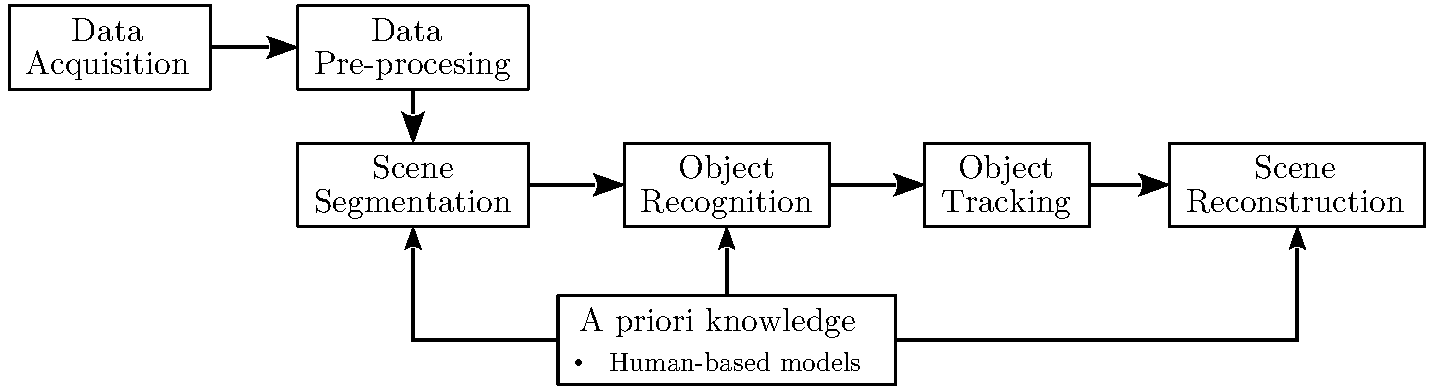
\includegraphics[width=\textwidth]{pipeline_scene_understanding_system}        
    \caption{Typical pipeline of a scene understanding system.}\label{fig:scene_understanding_systme_pipeline}
\end{figure}

Following the pipeline of Fig. \ref{fig:scene_understanding_systme_pipeline}, we can place the tasks of a scene understanding system into five general well-defined computer vision problems.

\begin{enumerate}[label=\roman*]
	\item \textbf{Image pre-processing}, whose objective is to remove the imperfections of an image generated by disturbances such as sensor noise or motion blur. Generally, we perform this task before passing it to a more complex algorithm. Image restoration and inpainting are some examples of this computer vision problem.
	
	\item \textbf{Image segmentation} is the process of partitioning an image into multiple (coherent) segments according to its features and properties. Depending on the application, we can formulate the image segmentation as the problem of classifying pixels with semantic labels (semantic segmentation), or partitioning of individual objects (instance segmentation), or both (panoptic segmentation).
	
	\item \textbf{Recognition} is a classic computer vision problem responsible for determining whether an image contains an object, characteristic, or exercise. Some variants of this problem are the classification, identification, and detection of objects from which many specialized tasks emerge. For example, content-based image search, pose estimation, optical character recognition, reading of 2-d codes, facial recognition, shape recognition, among others.
	
	\item \textbf{Motion analysis} is the problem that searches to estimate the speed of one or more points of interest within an image or 3-d scene by processing a sequence of images. Some examples of this task are egomotion, object tracking, pose estimation, and optical flow.
	
	\item \textbf{Scene reconstruction} is the problem related to the computation of a 3-d model from one or more images of a scene. This model is intended to be a description of the scene as close to reality as possible. 	
\end{enumerate}

These functionalities of computer vision and scene understanding systems are sought in the field of drones. UAVs (or drones) are flying engines that are increasingly present in our lives. We can find them in various sectors, such as the military, commercial or civil, where they can perform very specific tasks. However, in most cases, the development of such applications requires an expert pilot to control the aircraft. 

Commonly, the UAV control is achieved using conventional sensors, such as inertial sensors (IMUs) for orientation and GPS for position. The combination of information coming from these sensors in a flight computer allows the drones to remain stable in the air. However, IMUs present some drawbacks; for example, they suffer from bias error propagation due to the integral drift. On the other hand, the GPS signal is not always guaranteed; for example, the satellite signal may be low or unexisting in urban or indoor environments. A recurrent technique to enhance the drone's position accuracy implies the data fusion of pressure, ultrasonic, radars, and laser range-finders sensors \citep{Tomic.Schmid.ea:IRAM:2012}. The fusion of data can provide the advantages of each sensor. However, a significant limitation of these complex systems is flight time, a parameter mainly linked to the vehicle's total weight and the battery's capacity. Therefore, the use of multiple sensors onboard becomes expensive and impractical.

It is possible to extend the capabilities of a drone by integrating some visual sensor. Contrariwise to other sensors such as Lidars, visual sensors are passive, lightweight, and can acquire valuable information about the surrounding structures, including color and textures, and UAV's self-motion. The addition of visual sensors to perceive the environment has been a recurring strategy that has made these aerial robots more manipulable, safer, and even in some cases, autonomous \citep{He.Qiao.ea:CM:2018}, \citep{Kyrkou.Timotheou.ea:POT:2019}, \citep{Zhu.Wen.ea:arXiv:2020}.That means that the drone can perform a task without the need for human intervention. For this, the drone must be able to move without getting lost; moreover, it must interpret and understand the present scene so that it can be able to detect and avoid potential obstacles on its way. 

Today, one can use different visual sensors, such as monocular cameras \citep{Padhy.Xia.ea:TSC:2018}, stereo cameras \citep{Seitz.Curless.ea:CVPR:2006}, RGB-D cameras \citep{Huang.Bachrach.ea:RobR:2017}, fish-eye cameras \citep{Hrabar.Sukhatme:IROS:2004}, thermal cameras \citep{Gaszczak.Breckon.ea:IRCV:2011}, among others. This wide range of sensors offers more options and flexibility to deal with the problems mentioned above. The integration of such sensors in UAVs has allowed us to see the world from another perspective (literally), and the development of perceptual computer vision algorithms drives the technological improvement of these machines.

We know that today exist applications where vision algorithms have outstripped the capacity of human vision, so they have entirely replaced human personnel, for example, in industrial vision systems tasks, say, the inspection of production lines \citep{Malamas.Petrakis.ea:IVC:2003}. However, in other imaging areas, computer vision systems are only responsible for supplementing specific routines that require a considerable amount of time and experience from human experts. This discrepancy in the vision systems' performance is mainly related to the complexity of the task and the environment's conditions where the task is performed. In industrial vision systems, we can control the working conditions in most cases, while in areas such as robotics and unmanned aircraft (or UAV), with uncontrolled conditions and without large databases, computer vision algorithms bring a real challenge, even though the acquisition system is the same. 

\subsection*{Image Characteristics and Technical Locks in UAV Vision-based Applications}
%\markboth{Introduction}{Problem Statement}
%\section*{Computer Vision Problems in Drone Applications}
 
We can interpret the application and tasks made with drones as missions. Generally, such missions involve three central moments: take-off, navigation, and landing. The drone can perform such stages with conventional sensors; however, visual sensors provide valuable perceptual information about the environment.

Among the three moments that occur in drone missions, navigation and landing are the stages in which visual information (from onboard sensors) and computer vision algorithms most frequently intervene. In the landing stage, the needs and problems can be well-defined since it occurs at the end of the mission. Besides, we can control some conditions by adding pre-designed elements, such as landing targets or landing platforms, to facilitate the task. However, in the navigation stage, computer vision problems are mainly determined by the nature of drone applications.

Drone missions are generally carried out in complex scenes that change as the vehicle moves through space. For example, imagine all the scenarios that a delivery drone goes through during its mission: It can start its route in a commercial area, where the scenes mostly contain warehouses and big open spaces such as parking lots. Then, it could pass through rural areas, where the scenes can contain farmlands or wooded areas. Finally, when the drone reaches the delivery point within an urban zone, the environment may contain houses, trees, electricity, and telecommunications poles, among others. 

The mission through different environments generates considerable lighting changes and shadows, which results in overexposed and (or) dark images. Besides having no control over lighting conditions, we must also consider that the camera's position and orientation vary concerning the scene depending on the vehicle's height and orientation. Moreover, we must also consider the rolling shutter effect present in cameras using CMOS sensors. Therefore, the objects present in the images may have deformations because of the optic and the movement. Figure \ref{fig:img_drone_degradations} shows some images taken with a commercial drone in a natural setting. We can observe how the environment's lighting conditions and the nature of aerial applications introduce deformations to the images and objects present in the scene. 

Finally, we must not forget that we acquire the input images from an onboard camera, which is generally not stabilized; therefore, the images may be noisy or blurry. Such problems limit a computer vision algorithm to be globally efficient in all or most situations.


\begin{figure}[!ht]
    \centering
    \begin{subfigure}[b]{0.38\textwidth}
        \frame{\includegraphics[width=\textwidth]{Bebop_A}}
        \caption{Presence of shadows}
    \end{subfigure}
        ~ %add desired spacing between images, e. g. ~, \quad, \qquad, \hfill etc. 
      %(or a blank line to force the subfigure onto a new line)
    \begin{subfigure}[b]{0.38\textwidth}
        \frame{\includegraphics[width=\textwidth]{Bebop_B}}
        \caption{Saturations}
    \end{subfigure}
        ~ %add desired spacing between images, e. g. ~, \quad, \qquad, \hfill etc. 
      %(or a blank line to force the subfigure onto a new line)
    \begin{subfigure}[b]{0.38\textwidth}
        \frame{\includegraphics[width=\textwidth]{Bebop_C}}
        \caption{Change of scale}
    \end{subfigure} 
    \caption{Some examples of image degradations present in aerial imaging and UAV applications.}\label{fig:img_drone_degradations}
\end{figure}

In addition to the problems related to the complex scene conditions, we must consider that a drone is subject to sudden changes in the environment, such as wind gusts, which can affect its stability and modify the visual information given by the onboard sensors. In such cases, the vision algorithms for drone navigation must process the input information fast enough to provide answers and transform them into real-time decision actions.

Considering the conditions and problems of vision-based drone applications, we argue that a system for scene understanding is necessary for this kind of application. Moreover, scene understanding must use low-level information such as intensity, color, and texture in combination with perceptual tools to generate a robust image interpretation to the characteristic visual conditions of the aerial platforms. Among these classic computer vision problems, image segmentation is a crucial stage in the scene understanding pipeline. Image segmentation is a low-level task; however, it is critical for high-level applications such as classification, object tracking, reconstruction, and scene understanding. A robust segmentation to the changes and variants of complex environments allows the generalization of high-level tasks to new contexts and applications.

\section*{Image Segmentation State of the Art}
\markboth{Introduction}{Perceptual Information and Image Segmentation State of the Art}

Image segmentation has a long history in computer vision and is present in many applications in medicine, biology, robotics, and physics. Here, we present a brief review of the state-of-the-art segmentation methods taking into account the approach used and relationship with vision perception (a more detailed version of the state-of-the-art of segmentation methods appears in chapter \ref{ch:perceptual_object_boundaries_detection}, section \ref{sec:SoA_segmentation_methods}). For this purpose, we divide the image segmentation techniques into classical methods and Artificial Intelligence (AI) methods. 
%\cite{Khan:IJIG:2013}

\subsubsection*{Classical Image Segmentation Techniques} 
Classical image segmentation methods can be organized into two groups: those that identify similarities or those that identify discontinuities \citep{Zaitoun.Aqel:ICCMIT:2015}. The first kind of approach detects similar pixels in the image based on some specific threshold or criteria for split-merge and growing regions. The second category of methods tries to find the boundaries between dissimilar pixels in the image. A more specific classification according to the technique used divides segmentation methods into Threshold-based, edge-based, region-based, watershed-based, clustering-based, PDE-based, and Graph-based \citep{Zaitoun.Aqel:ICCMIT:2015}.

\textbf{Threshold-based} algorithms are one of the simplest image segmentation techniques. The threshold operation divides the image by comparing the intensity of the pixels to a specific threshold value\citep{Sezgin.Sankur:EI:2010}. This kind of method can only segment images into background and foreground based mainly on the intensity pixel information. This property is convenient when there is a significant contrast difference between the objects and the background. The major challenge of such approaches is the choice of the threshold value. The simplest option is to use a global threshold for the whole image; however, this option fails when the illumination in the image is uneven. Local thresholding methods solve this problem by proposing multiple thresholds \citep{Niblack:ImageProcc:1986}, \citep{Sauvola.Pietikainen:ICPR:2000}; however, the computation time can increase considerably. One of the most popular approaches in this category that automatically determine the threshold value is Otsu's method \citep{Otsu:SMC:1979}.

The \textbf{Edge-based} segmentation methods attempt to solve the image segmentation problem by detecting edges in an image according to the differences in texture, contrast, grey level, color, saturation, and other properties \citep{Saini.Arora:IJICT:2014}. Some of the more well-known methods in this category employ operators that use the first and second derivatives of the image to identify abrupt changes in the intensity of the image, for example, the Sobel \citep{Sobel.Feldman:SAIL:1990}, Roberts \citep{Roberts:Thesis:1963}, Gradient \citep{Maitre:Book:2003}, Prewitt \citep{Prewitt:PPP:1970}, and Laplacian \citep{Marr.Hildreth:PRS:1980} operators. On the other hand, one of the state-of-the-art reference work is the Probability-boundary (Pb) \citep{Malik.Belongie.ea:IJCV:2001},  which uses the intensity and color, and texture information to obtain the edges of the image. 

The \textbf{Region-based} segmentation methods partition the image into similar regions according to predefined criteria. Depending on the strategy used to arrive at the final segmentation, they can be organized into region growing and splitting and merging techniques \citep{Sezgin.Sankur:EI:2010}. Region growing techniques define a group of seed pixels from which regions start to grow \citep{Zucker:CGIP:1976, Adams.Bischof:TPAMI:1994}. Regions grow by appending to each seed pixel those neighboring pixels that have predefined properties similar to those of the seed pixels (e.g., intensity or color). Regions stop growing when they reach a particular predefined stop criterion (e.g., size or shape of the region).
Conversely, splitting and merging techniques do not require seed pixels. This technique successively divides the image into quadrants based on a homogeneity criterion, then similar regions are merged to form the final segmentation. This strategy includes the quad-tree data structure \citep{Horowitz.Pavlidis:ACM:1976}, which means a parent-child node relationship.
In practical applications, the region growing and splitting and merging algorithms are usually used in combination \citep{Ikonomatakis.Plataniotis.ea:ICDSP:1997}. This combination is more effective for the segmentation of complex scenes defined by some complex objects or the segmentation of certain natural scenes, such as image segmentation with insufficient prior knowledge.

The \textbf{Watershed-based} segmentation is a technique that utilizes image morphology and combines the characteristics of edge- and region-based methods described above. First, this method computes the gradient of an image. We can see this gradient as a map that reflects the topography of the image through the intensity values of the pixels. Then, segmenting an image is equivalent to flooding the topography from a group of seed pixels, where the edges of the image appear as the highest ridges where the flood water meets \citep{Meyer.Beucher:JVCIR:1990, Beucher.Meyer:Book:1993}. The watershed method is strictly linked to hierarchical segmentation methods \citep{Najman.Schmitt:PAMI:1996}. This feature of hierarchical dependence complexifies the efficient implementation in embedded processors. Many strategies introduce other definitions of the watershed transform to solve the complexity problem,  which simplifies and accelerates its computation \citep{Roerdink.Meijster:IOS:2000} , \citep{Dejnozkova.Dokladal:ICASSP:2003}, \citep{Chabardes.Dokladal.ea:ICIP:2016}.

Another alternative to obtain the segmentation of an image is by using clustering methods. The \textbf{clustering-based segmentation} methods are unsupervised techniques that classify the image pixels into clusters (disjoint groups) with similar features. The objective of pixel clustering is to maximize intra-class differences and minimize intra-class differences; that is, the pixels in each class should be as similar as possible, and those in the different groups should be as different as possible \citep{Steinley:BJMSP:2006}. The k-means technique is known as a hard-clustering technique since each pixel can belong only to one class. Fuzzy algorithms (soft-clustering) relax that condition, and each data point can belong to more than one cluster. This behavior is suitable in applications where there are no crisp boundaries between objects, such as tissue classification \citep{Caldairou.Passat.ea:PR:2011} and tumor detection \citep{Preetha.Suresh:CCT:2014}. Among the soft-clustering methods, fuzzy C-means clustering \citep{Dunn:JC:1973} is one of the most used.

\textbf{PDE-based} segmentation methods use Partial Differential Equations to model the image contours and obtain an image segmentation.  Active Contour Model (or Snakes) transform the segmentation problem into
PDE. Some famous methods of PDE used for image
segmentation are Snakes \citep{Kass.Witkin.ea:JCV:1988}, Level-Set \citep{Osher.Sethian:JCP:1988}, Fast Marching \citep{Forcadel.LeGuyader.ea:NA:2008}, and Mumford Shah method \citep{Mumford.Shah:CPAM:1989}. One of the main problems of these methods is the high computational time for the resolution of the PDE, which limits its use on embedded platforms. This limitation has been addressed in the implementation level through architectures that allow multi-core parallel calculation \citep{Dejnozkova.Dokladal:ICVIE:2003, Dejnozkova.Dokladal:ICASSP:2004}.

The last group of classical methods for image segmentation is \textbf{Graph-based}. These methods make use of graph theory to represent the image as a graph.  Typically, a pixel or a group of pixels are associated with nodes, and the edge weights define the affinity between neighboring pixels. Then, we can partition the graph according to a criterion designed to model good clusters. Each resulting partition of nodes is considered a segmented object in the image. Some popular algorithms in this category are normalized cuts \citep{JianboShi.Malik:PAMI:2000}, random walker \citep{Grady:PAMI:2006}, minimum cut \citep{Wu.Leahy:PAMI:1993}, isoperimetric partitioning \citep{Grady.Schwartz:PAMI:2006}, and minimum spanning tree \citep{Zahn:TC:1971}. Some of the segmentation methods can combine strategies. For example, spectral clustering \citep{Ng.Jordan.ea:NIPS:2001} uses the graph theory and the similarity of the graph edges to cluster the image pixels into coherent regions. On the other hand, \citep{Cousty.Bertrand.ea:PAMI:2009} define the watershed cuts cut on edge-weighted graphs using the Minimum Spanning Forest.

This group of approaches and techniques (known as classical, conventional, or traditional) can use structural, stochastic, or hybrid techniques to segment an image. Structural techniques require structural data from the image, such as distributions, histograms, pixel density, or color distribution. Stochastic techniques require information about the discrete values of the pixels. Machine learning methods, such as the clustering techniques, fall into this category. Finally, hybrid techniques may use structural information of image regions and the discrete values of the pixels of the whole image for the segmentation. The choice of the method to segment an image depends on the type of image and the type of segmentation that we seek to obtain (for example, over-segmentation or segmentation to pixel precision). Regardless of this, we consider it essential to consider the perceptual elements of the data to achieve a meaningful interpretation of the scene.

\subsubsection*{AI Image Segmentation Techniques} 
The \textbf{Artificial Neural Networks- (ANN) based} techniques (a.k.a. Deep Learning (DL) techniques) are probably the most widely used methods today because of their efficiency and accuracy. They are part of the supervised techniques, i.e., they require an annotated database for training, validation, and testing. In ANN-based methods, every neuron corresponds to the pixel of an image, which means the image is mapped to the neural network. Then, the image in the form of the neural network is trained using labeled data to find the connection between neurons (pixels). Lastly, the new images are segmented from the trained model. 

In recent years, neural network techniques (also known as deep learning (DL) techniques) have led to new models for image segmentation. We can classify these methods roughly according to the architecture they use. Convolutional Neural Networks  (CNNs) are among the most widely used and successful architectures in computer vision. This model, initially proposed by \cite{Fukushima:BC:1980}, is inspired by the model of the human visual cortex. Generally, CNNs contain convolution layers, non-linear layers (or activation functions) for feature mapping and pooling layers. Some of the best-known CNNs in the literature include LeNet \citep{Lecun.Bottou.ea::1998}, AlexNet \citep{Krizhevsky.Sutskever.ea:NIPS:2012}, VGGNet \citep{Simonyan.Zisserman:arXiv:2015} and ResNet \citep{He.Zhang.ea:ICVPR:2016}. 

Due to their characteristics, CNNs require dense layers and a large number of parameters, which makes them highly expensive. Fully Convolutional Networks (FCN) \citep{Long.Shelhamer.ea:CVPR:2015} solve this drawback by stacking several convolution Layers with similar padding to preserve the dimension and output a final segmentation map of the same size as the input image. Some of the best-known models are VGG16 and GoogleNet \citep{Szegedy.Liu.ea:arXiv:2014}.

Other deep learning backbones are the Encoder-Decoder and Auto-Encoder architectures. This type of model is known as two-stage networks. The first stage, encoding, compresses the input information into a space-latent representation, while the second stage, decoding, predicts an output from the representation. Some examples of networks that follow this architecture are DeConvNet \citep{Noh.Hong.ea:ICCV:2015}, SegNet \citep{Badrinarayanan.Kendall.ea:PAMI:2017}, U-Net \citep{Ronneberger.Fischer.ea:MICCAI:2015}, W-net \citep{Xia.Kulis:arXiv:2017}, Linknet \citep{Chaurasia.Culurciello:VCIP:2017}, among others.

Object detection and image segmentation are complementary tasks in computer vision. Similarly, exist architectures designed for object detection, such as Regional CNN (R-CNN), which have been successfully adapted for image segmentation. Some examples are the Faster R-CNN \citep{Ren.He.ea:PAMI:2017}, Mask R-CNN \citep{He.Gkioxari.ea:PAMI:2020} and Masklab \citep{Chen.Hermans.ea:CVPR:2018} architectures. The operation principle of these architectures is to extract the features of certain regions of interest to infer the class and the coordinates of the bounding box of the object.

A very recent family of architectures are those based on Generative Adversarial Networks (GANs) \citep{Goodfellow.Pouget-Abadie.ea:NIPS:2014}. This architecture consists of two networks, a generator, and a discriminator. The generator has the task of reproducing distributions similar to the real samples. On the other hand, the task of the discriminator is to distinguish the fakes samples from the real ones. GANs models include Convolutional-GANs \citep{Radford.Metz.ea:arXiv:2016}, Conditional-GANs \citep{Mirza.Osindero:arXiv:2014}, and Wasserstein-GANs \citep{Arjovsky.Chintala.ea:arXiv:2017}.

Other popular DL architectures for image segmentation include Feature Pyramidal Networks (FPN) \citep{Lin.Dollar.ea:CVPR:2017}, which takes a multi-scale approach, or hybrid ones that combine classical methods such as the Active Contour Model \citep{Kass.Witkin.ea:JCV:1988} and CNNs, or the watershed transform in the deep watershed architecture \citep{Bai.Urtasun:CVPR:2017}. 

The literature on methods based on DL architectures for image segmentation is vast. For a more detailed survey of the state of the art of ANN-based methods for image segmentation, please check \citep{Sultana.Sufian.ea:KBS:2020} and \citep{Minaee.Boykov.ea:PAMI:2021}.

%\citep{Kelm.Rao.ea:CAIP:2019}
AI-based image segmentation methods are experiencing popularity and growth that has benefited from advancements in computing power and the recent creation of publicly accessible annotated databases. However, its use in particular applications where there are not (yet) large enough annotated databases is complicated. Furthermore, despite the performance in challenging benchmarks, in many cases, the interpretability of the results of these methods remains open questions.

\subsubsection*{Vision-based UAV Navigation Related Works}
In the literature, we can find many works that deal with computer vision for drone navigation. The different approaches are strongly related and motivated by the application's aim and the conditions in which the task is developed. We can differentiate two main vision-based techniques for UAV navigation; 1) localization and mapping and 2) obstacle avoidance.

Simultaneous Localization and Mapping (SLAM) falls within the first group techniques, where drone navigation is a consistent result. This technique estimates the drone's local pose and builds a 3-d model of its surroundings employing visual sensors. Visual Odometry (VO) \citep{Scaramuzza.Fraundorfer:RAM:2011} is responsible for the robot motion estimation while the maps are built with occupancy grid algorithms \citep{Thrun.Bu:AI:1996}. According to the image information used to perform a SLAM, we can classify these approaches into feature-based methods, which extract a set of image features (e.g., lines, points) in a sequence of images, and direct-based methods, which make use of the image intensity information to estimate the structure and the motion of the robot \citep{Taketomi.Uchiyama.ea:TCVA:2017}. The importance of a correct segmentation of the image is that we can also create a depth chart of the scene from it and consequently achieve the visual odometry \citep{Drouyer:Thesis:2017, Drouyer.Beucher.ea:MMASP:2017}. 

The use of SLAM techniques for UAV navigation presents remarkable advantages. Feature-based methods can use various feature detectors, which typically count with an optimization stage to produce fast algorithms. Direct-based methods have the advantage of being robust to image degradations; they can lead better with images with texture and blurred zones; besides, the map produced is of an acceptable resolution. Interestingly, the strengths of the first group of methods are the weak points of the second and vice versa. A method that tries to gather the benefits of both approaches is the Semi-direct Visual Odometry \citep{Forster.Pizzoli.ea:ICRA:2014}; however, in general, the state-of-the-art SLAM methods is more mature in the autonomous vehicle environment \citep{Singandhupe.La:IRC:2019}.

There are approaches for drone navigation that, in parallel to SLAM, favor the avoidance of obstacles. This capability is essential for achieving free collision missions in both indoor and outdoor environments. A recurrent solution, as we early mentioned, is the multi-sensor data fusion. \cite{Gageik.Benz.ea:ACCESS:2015} present a platform using low-cost ultrasound and IR sensors; however, despite the obtained results, it utilizes several sensors to retrieve environment information, and yet, it does not get a perceptual representation of the scene due to the low resolution and perceptive capacity of the sensors. On the other hand, vision-based techniques for obstacle avoidance could detect obstacles and, in some cases, recognize and classify the object representing the obstacle \citep{Li.Ye.ea:IROS:2016}. 

We can classify the visual methods for avoidance of obstacles into two groups. The first, SLAM-based techniques, make use of the principles stated above. The 3-d reconstruction provides accurate and sophisticated maps and allows the air vehicle to travel with more information about the environment. In \citep{Moreno-Armendariz.Calvo:ICMEAE:2014}, takes this advantage to develop an obstacle avoidance approach for static and dynamic obstacles. The second group is the flow-based methods which historically, were inspired by the navigation of insects such as bees \citep{Srinivasan.Gregory:PTBS:1992} or flies \citep{Franceschini.Ruffier.ea:InTech:2009}. Many insects in the wild identify obstacles through the intensity of light. During the flight, their eyes produce an optical flow that provides accurate spatial information. Currently, there are also works inspired by the behavior of the human eye \citep{Al-Kaff.Meng.ea:IVS:2016}. The technique measures the object size from the idea that objects in the robot's vision field are more significant as the obstacle is close.

In general cases, obstacle avoidance techniques are strongly linked to the camera parameters and acquisition conditions. The algorithms are often fine-tuned. Given the condition, a drone operates in an environment without prior knowledge and under uncontrolled conditions. Hence some more general, unsupervised methods are needed.

Today, the most efficient algorithms are those based on Neural Network (NN) architectures and supervised learning techniques. Nevertheless, these techniques have remarkable disadvantages that question their usability and applicability in real-life drone missions \citep{Treboux.Genoud.ea:IWBIS:2018}. From a practical and even economic point of view, there is a limit to the number of applications in which we can use supervised methods given the fact that we need a lot of annotated data \citep{Xu.Wang.ea:CEA:2020}. The collection and the correct labeling of data representing a problem are valid only for a small number of applications.

The need for abundant information comes with high computational times required for model learning, ranging from a couple of hours to weeks. Of course, we can minimize this variable by increasing our machines' computing power; however, today, only those with large computing infrastructures can afford to train models with hundreds of billions of parameters.  

The above statement introduces the next disadvantage of deep neural network-based learning models: hyperparameters. We can roughly divide hyperparameters into two categories: 1) optimizer hyperparameters, which include the learning rate, the batch size, and the number of epochs, and 2) model-specific hyperparameters, which include the number of hidden layers, the first hidden layer, and the number of layers. Choosing the appropriate hyperparameters plays a crucial role in the success of neural network architectures because they control the learning algorithm's behavior, define the network structure, and define how the network is trained. Although there are methods to optimize their choice, generally, this task is a heuristic process, and their fine-tuning is a function of the specific application. It is possible to follow some rules based on experience, copy the same values from some other problem or make the setting by trial and error, though we cannot know the best value for a hyperparameter.

We can thus conclude that it is crucial to have the means to understand the scene, depending less on the parameters fixed in advance or the data sets prepared for a particular mission. In the following paragraphs, we present the contribution of this thesis to this issue.


%Nowadays, there is a wide variety of image segmentation techniques, some considered general-purpose and some designed for specific images.  On the other hand, \cite{Zaitoun.Aqel:ICCMIT:2015} propose a two-group classification: layer-based and block-based segmentation methods. Under these two taxonomies, we focus on classical or block-based segmentation methods. More specifically, we perform region-based segmentation and boundary-based segmentations.

\section*{Scope of the Thesis}
\markboth{Introduction}{Scope of the Thesis}
%First of all, this thesis work is motivated mainly by my profile and interests in robotics and control theory, specifically in air vehicles. 

The interaction between computer vision and applications made with unmanned aerial vehicles is extensive. This collaboration has generated new methodologies and approaches, both theoretical and practical, but has also given way to new research questions. 


Knowing the fundamental limitations of aerial robots and the complexity of drone applications, we explore computer vision theory to propose algorithms that improve and provide assistance in drone navigation tasks. In this sense, we are interested in studying the scene's perceptual information for their treatment and interpretation.

We focus primarily on the vision processing problems: object segmentation and recognition. We argue that two computer vision tasks are crucial for image understanding and have to be carefully treated in complex, uncontrolled environments. From this perspective, we focus on using low-level image features to extract perceptual information. 

Based on Fig. \ref{fig:scene_understanding_systme_pipeline} and considering the scope of the work in this thesis, we propose a new pipeline for scene understanding systems. In this new pipeline, the pre-processing of the image involves its perceptual decomposition, while the segmentation stage considers the perceptual elements of the image. The proposed pipeline for scene understanding is showed in Fig. \ref{fig:my_scene_understanding_systme_pipeline}. The peculiarity of this pipeline is that it eliminates the dependency on the a priori models, at least for the tasks of segmentation and image recognition (tasks that we study in this thesis). 

\begin{figure}[!ht]
    \centering
    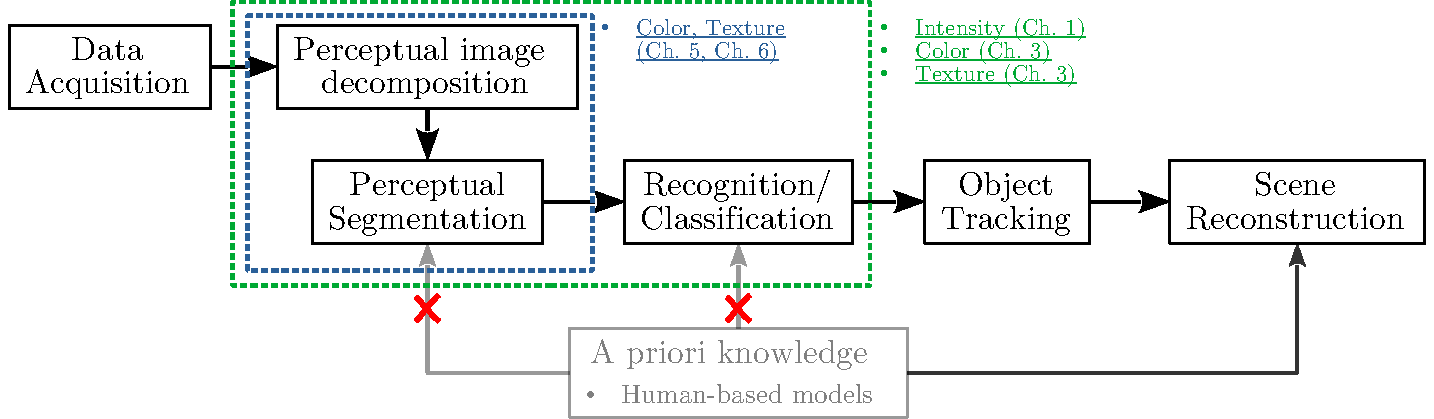
\includegraphics[width=\textwidth]{my_pipeline_scene_understanding_system}        
    \caption{Proposed pipeline of a scene understanding system.}\label{fig:my_scene_understanding_systme_pipeline}
\end{figure}

Throughout this work, we develop algorithms that are capable of handling a variety of real-world conditions. All these algorithms aim to segment the physical objects that we, as humans, define as perceptually interesting. For this purpose, we use intensity, color, and texture image information to extract low-level primitives, such as contours. In Fig. \ref{fig:my_scene_understanding_systme_pipeline}, we show the stages of scene understanding that we study in this thesis and the low-level primitives involved in the task: in green, the recognition and classification of objects use intensity, color, and texture, and in blue, the perceptual segmentation uses color, texture and the relationship between them. We use these primitives in conjunction with statistical and geometric tools from computer vision and signal theory, such as anomaly detector, optimal transport, and Gabor functions. Instead of using supervised methods, we focus on decomposing the image information from the point of view of signal theory and physics to use it later on non-supervised or mathematical morphology methods.
%So it is worth mentioning that the practical aspect linked to the implementation and the generation of solutions in real-time are not a priority. The developed algorithms provide solutions to the recognition and scene understanding problem's variants, such as the classification, identification, and detection of objects from a qualitative point of view, always looking for the application's physical meaning. 

Regarding the nature of the input data, we use only gray-level or color images as input information, favoring monocular cameras among the wide range of visual sensors reviewed previously. This choice allows replicating the algorithms with low-cost cameras that can be easily embedded in a drone.

%One last point about the focus of this work is about the type of computer vision techniques. The algorithms proposed in this thesis are based on traditional computer vision techniques, that is, non-deep learning techniques. This decision is consistent with drone applications' nature, where there are not necessarily rich enough annotated databases to apply the most sophisticated artificial intelligence models.

\section*{Contributions of the Thesis}\label{sec:objectives_of_the_thesis}
\markboth{Introduction}{Contributions of the Thesis}

%In this Ph.D. thesis, we aim to develop general computer vision algorithms considering the challenges and needs of UAV navigation. 

The primary objective of this Ph.D. thesis is to propose a new methodological framework for decomposing images before segmenting and detecting objects in the context of the scene understanding. The idea is to apply this methodological framework to assist in control and decision-making in drone navigation tasks. Therefore, the framework must be robust to image degradations existing in environments with uncontrolled conditions, in addition to being independent of the choice of specific parameters for its operation.

%During the thesis, we consider many specific drone tasks, such as:
%
%\begin{enumerate}[label=\roman*]
%	\item \textbf{Recognition} is a classic computer vision problem responsible for determining whether an image contains an object, characteristic, or exercise. Some variants of this problem are the classification, identification, and detection of objects from which many specialized tasks emerge. For example, content-based image search, pose estimation, optical character recognition, reading of 2-d codes, facial recognition, shape recognition, among others.
%	\item Environment awareness.
%	\item Detection and avoidance of obstacles.
%	\item Identification and following of targets.
%\end{enumerate}
%Given these tasks, the work focuses on the scene understanding problem. To deal with this problem, 
We extend the study of primary image information such as intensity, color, texture, and texture color and low-level image primitives such as contours. Therefore, some secondary objectives involve building a representation of the image in feature space using concepts from signal theory, geometry, and statistics, in addition to concepts from human perception. We seek to validate the proposed image representation using unsupervised approaches in real applications following traditional machine learning and segmentation algorithms.

Figure \ref{fig:general_diagram_framework} shows a general flowchart of the contributions of this thesis. The first stage of the flowchart shows low-level information and the methods we use to extract it; here, we work with intensity, color, texture, and the relationship between color and texture. The second stage of the diagram shows the different representations of the image obtained from the perceptual information contained in the primitives. Finally, the diagram's third section collects the different applications used to validate the image's feature spaces constructed in this thesis. Although the idea of a single framework itself is an ambitious goal, in this thesis, we present several algorithms that apply the proposed methodology with one or more features to solve different computer vision problems such as object detection and recognition, image retrieval systems, perceptual object boundaries detection, and image segmentation.

The interest of obtaining a representative space of the image information from low-level hand-made features lies in the possibility of using it in a semi-supervised pipeline. By injecting annotated information into the frame, it might make generalizations and obtain medium- or high-level features such as the importance of color and texture information to a human when segmenting an image. 

\begin{figure}[!ht]
    \centering
    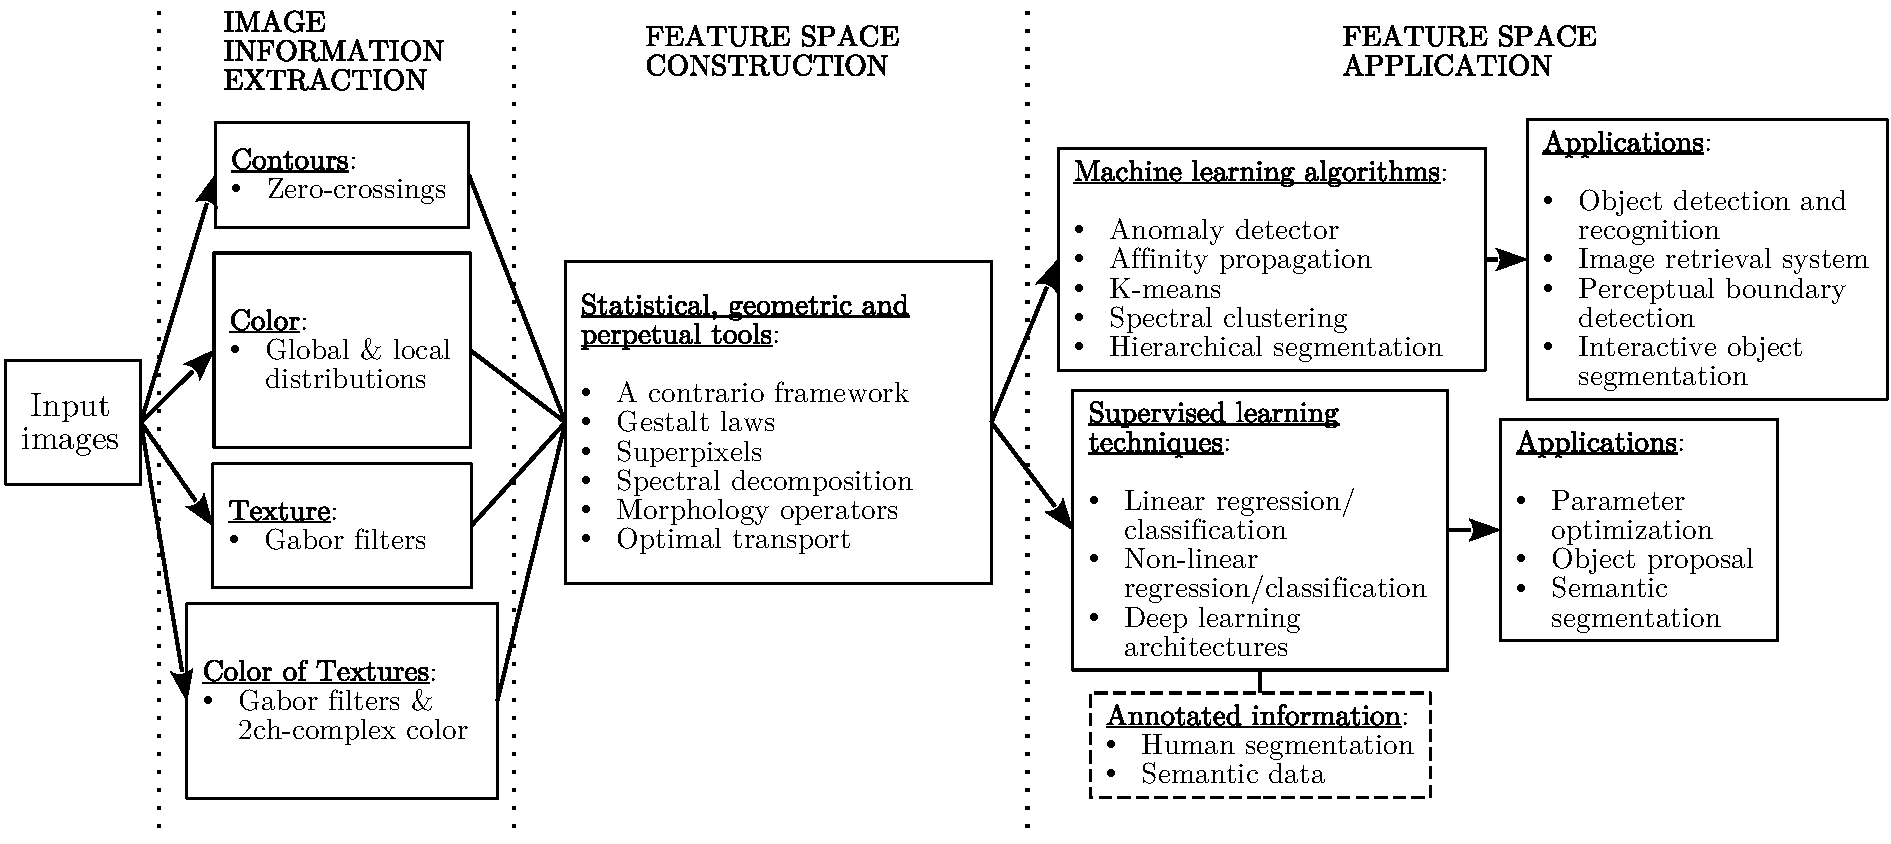
\includegraphics[width=\textwidth]{general_framework_diagram}        
    \caption{Flowchart of thesis contributions.}\label{fig:general_diagram_framework}
\end{figure}

Specifically, the contributions of this thesis include:

\begin{itemize}
	\item A novel non-parametric framework for fully unsupervised object detection robust to the image degradations present in complex, uncontrolled environments (chapter \ref{ch:landing_target_detection}).
	\item A qualitative and quantitative study between the most popular measures in the comparison of distributions (chapter \ref{ch:similarity_measures}). 
	\item An unsupervised image retrieval system based on global color/texture information (chapter \ref{ch:similarity_measures}).
	\item Extensive analysis of Gabor filters and their properties in the space-frequency domains (chapter \ref{ch:spectral_image_decomposition}).
	\item Generation of a feature space that includes the color and texture information of an image (chapter \ref{ch:complex_spectral_image_decomposition}).
	\item Unsupervised framework for natural image segmentation (chapter \ref{ch:perceptual_object_boundaries_detection}).
\end{itemize}

Finally, this thesis aims to show that traditional computer vision methods are (still) a reliable option to develop object detection and recognition for relatively complex tasks. We place this argument in the current context of computer vision, where there are hundreds of algorithms based on Neural Networks and Artificial Intelligence. Besides the NN and AI algorithms for image segmentation and object detection are highly performant, they lack a physical (and in many cases logical and argued) interpretation of its results. Furthermore, these algorithms are in trouble when it comes to image analysis of complex scenarios or applications where there is no database rich enough to do the learning process.


\section*{Organization of the Document}
\markboth{Introduction}{Organization of the Document}

To communicate our proposal and the objectives mentioned above in a clear and structured way, we present a thematic and chapter organization of the document. The thematic organization follows, to some extent, the complexity of the three low-level image information we used during this thesis: intensity, color, and texture. Then, we can identify three main parts in this thesis.

\begin{enumerate}
	\item The first part is dedicated to studying the intensity information of the image, in which we review in detail some of the classic methods for obtaining image contours. We use this information in conjunction with the \textit{a contrario} method and the Gestalt organizing laws to detect and identify landing targets. This part includes chapter \ref{ch:landing_target_detection}. 
	\item The second part main topic is studying the properties of color and texture of an image. We are interested in the global distribution of this information and the existing metrics to measure the similarity between the distributions; we apply and validate these concepts in two image retrieval systems. This part covers from chapter \ref{ch:color_texure_representations} to chapter \ref{ch:spectral_image_decomposition}.
	\item The third part extends the study of color and texture in images, exploding the local distribution of these primitives and studying the influence of color information on the generation of textures in an image. We propose a multi-spectral image decomposition helpful on the object segmentation tasks using classic clustering algorithms and for the generation of high-level texture features. Moreover, we propose a completely unsupervised framework for the detection of perceptual boundaries. We also explore different strategies to obtain the segmentation of natural images using the obtained perceptual boundaries. This part includes chapter \ref{ch:complex_spectral_image_decomposition} to chapter \ref{ch:perceptual_object_boundaries_detection}.
\end{enumerate}

The organization by chapters is structured as follows:

\begin{itemize}
	\item \textbf{Chapter \ref{ch:landing_target_detection}} addresses the bases of the Gestalt theory, including the grouping laws and the Helmholtz principle. We formalize these concepts of human perception mathematically and formulate a non-parametric algorithm that follows an unsupervised framework based on an image's contours. We use the developed framework in the autonomous drone landing problem, specifically detecting and identifying landing targets.  The chapter also presents a review and a quantitative comparison of different traditional methods for extracting image contours.
	
	\item \textbf{Chapter \ref{ch:color_texure_representations}} presents a detailed review of the different ways to represent the color and texture information in an image. The chapter contains a review of various color spaces and their main properties and an introduction to the different techniques for characterizing textures in the literature. Such information is of relevant importance in constructing the framework and the approaches to measure similarity between distributions.
	
	\item \textbf{Chapter \ref{ch:similarity_measures}} presents the analysis between different similarity measures between distributions, showing the advantages and disadvantages of each of them. In particular, we focus on the theory of optimal transport through the Earth Mover's Distance. We show the advantages of this metric over traditional similarity measures using an image retrieval system based on an image's global color and texture information.
	
	\item \textbf{Chapter \ref{ch:spectral_image_decomposition}} explores the physical and human perception aspects of Gabor's filters. We show the steps involved in designing an optimized and efficient Gabor family of filters. The proposed filter family models and captures the texture information through an energy-efficient decomposition of the image. Such spectral decomposition of the image deals with Heisenberg's uncertainty principle. The chapter presents the description of parameters that allow complete customization of the filter family according to the application.
	
	\item \textbf{Chapter \ref{ch:complex_spectral_image_decomposition}} brings an analysis of the texture information present in color images, showing the strong relationship between those two features. Using the spectral analysis of an image with the previously defined Gabor filters, we generate a feature space that simultaneously captures the color and texture information. We show the richness of such feature space by performing unsupervised image segmentation only using simple clustering techniques. Moreover, we show some novel high-level texture features resulting from the spectral image decomposition.
	
	\item \textbf{Chapter \ref{ch:perceptual_object_boundaries_detection}} introduces a framework for detecting perceptual boundaries of objects present in natural images. This framework brings together concepts addressed in this document, such as the spectral decomposition of images, the optimal transport as a true metric, and the relationship between color and texture information. Besides, using the hierarchical segmentation technique, we segment natural images in an unsupervised manner. We perform a quantitative and qualitative validation of our method using a known database.
	
%	\item \textbf{Chapter \ref{ch:general_conclusion}} contains the general conclusions of the thesis and addresses the different possible research lines as a continuation of this work.
	
\end{itemize}


	\cleardoublepage
	% created on 28/07/2020
% @author : ebazan
\part{Image Contours}\label{part:image_contours}

\section*{Introduction}
The general objective of this thesis is to propose a vision-based framework for the navigation aid of UAVs. We consider that the understanding of scenes is an important aspect for the elaboration of this framework. The proposal then is to build a framework that obtains perceptual information using low-level primitives and low-level features of the image. 

In this first part of the thesis, we focus only on the study of the contours of an image and its properties. We review some concepts of human perception, such as Helmholtz's principle, and we interpret them and apply them to the contours extracted from the image. More specifically, we use the image contour information in an \textit{a contrario} approach and some of the grouping laws from the Gestalt theory to perform the detection and identification of objects. We use this algorithm for the autonomous drone landing task. The objects to be identified are a series of landing targets specifically designed for this problem.

The main contributions of this first part are:

\begin{enumerate}
	\item Study and comparison of different classical approaches to image's contours detection.
	\item A new methodology for searching and interpreting perceptual information using the a contrario method and Gestalt theory.
	\item A framework for fully unsupervised landing target detection robust to the image degradations present in the autonomous landing task.
	\item An algorithm for the generation of coded landing targets.
\end{enumerate}


\chapter{Unsupervised Object Detection for UAV Autonomous Landing Task} \label{ch:landing_target_detection}

Associated publications: \vspace{-2mm}

\begin{itemize}
	\item \citep{Bazan.Dokladal.ea:ACIVS:2018}. << Unsupervised Perception Model for UAVs Landing Target Detection and Recognition >>. In: \textit{International Conference on Advanced Concepts for Intelligent Vision Systems}. Springer, pp 233-244.
	\item \citep{Bazan.Dokladal.ea:RFIAP:2018}. << Non supervised perceptual model for target recognition in UAVs >>. In: \textit{Reconnaissance des Formes, Image, Apprentissage et Perception RFIAP}, Marne la Vallée, France.
\end{itemize}

\section*{Résumé}
\noindent Dans ce chapitre, nous abordons le problème de l'atterrissage autonome des drones, et plus précisément, la détection et la reconnaissance robustes d'une cible d'atterrissage unique dans un environnement extérieur. Le défi est de savoir comment gérer les images dans des conditions de lumière non contrôlées, impactées par les ombres, le changement d'échelle, la perspective, les vibrations, le bruit, le flou, entre autres. Nous introduisons un modèle robuste non supervisé qui nous permet de détecter et de reconnaître une cible, de manière perceptuelle, en utilisant les principes de Gestalt de non-accidentalité et de regroupement. Notre modèle extrait les contours de la cible d'atterrissage sous forme de valeurs aberrantes à l'aide du détecteur d'anomalies RX et en calculant la proximité et une mesure de similarité. Enfin, nous montrons l'utilisation du code de Hamming de correction d'erreurs dans la génération des cibles d'atterrissage et pour réduire les erreurs de reconnaissance.

\section*{Abstract}
\noindent In this chapter, we tackle the problem of UAVs autonomous landing, and more precisely, the robust detection and recognition of a unique landing target in an outdoor environment. The challenge is how to deal with images under non-controlled light conditions impacted by shadows, change of scale, perspective, vibrations, noise, blur, among others. We introduce a robust unsupervised model that allows us to detect and recognize a target, in a perceptual-inspired manner, using the Gestalt principles of non-accidentalness and grouping.  Our model extracts the landing target contours as outliers using the RX anomaly detector and computing proximity and a similarity measure.  Finally, we show the use of error correction Hamming code in the generation of landing targets and to reduce the recognition errors. 


\section{Introduction}\label{sec:introduction_ch1}
Nowadays, the target detection for the autonomous landing of UAVs is a recurring subject in the industrial sector. This task is crucial so that applications such as air parcel delivery can be developed. Some strategies to address this problem is the creation of landing stations; infrastructures that could contain external elements, such as GPS, infrared markers or telecommunication sensors, which serve to locate and differentiate the landing zone from other areas. This option may be feasible for small-scale applications, however, in applications that require multiple landing points, this becomes impractical.

Instead, we propose a monocular vision-based system for the detection and identification of custom landing targets. For this we imagine the situation when a drone is ready to land as follows: first, the drone reaches a certain horizontal/vertical distance from a possible landing target, then it activates the visual system and analyzes the scene where there may be a target; if the drone recognizes a pattern as a landing target and the ID is correct, the drone lands. The figure \ref{fig:visionbased_landing_problem_sketch} represents the actions that a drone must perform to land at the correct point. The use of vision systems for the target detection provides advantages such as the independence of special on-board sensors for the detection of infrared markers and the  continuous operation in areas with low or no GPS coverage. 

\begin{figure}[!ht]
    \centering
    
\includegraphics[width=0.45\textwidth]{problem_statement}        
    \caption{Graphic representation of the two stages involved in vision-based autonomous landing: 1. Approach to the landing zone; 2. Detection and recognition of the landing target.}\label{fig:visionbased_landing_problem_sketch}
\end{figure}

Notwithstanding, the use of visual systems in outdoor environments presents challenges as there are many uncontrolled variables that affect and impair the task of detecting objects. The main problems to face in the aerial landing target detection task are: the non-controlled light changes that generate shadowing, reflectance and saturation on the surfaces; the perspective and distance of the camera that deforms the objects; the motions and vibrations that blur the images and; the noise generation by a low-quality sensor.

The detection of the landing target can be viewed as an image segmentation problem, where there is a wide range of developed methods. The variational framework \citep{Mumford.Shah:CPAM:1989}, offers an optimal general method for image segmentation; however, its mathematical complexity and the constant selection of fidelity and a regularization parameters makes its use complex. Also, the number of iterations needed to find the optimal solution avoid having results in real-time. Conversely, threshold-based methods have been used for the detection of landing targets \citep{Lacroix.Caballero:IROS:2006}, \citep{Lange.Sunderhauf.ea:SIMPAR:2008} for its ease of use. However, for a good detection, its use is limited to indoor spaces, where the light conditions are controlled \citep{Araar.Aouf.ea:IROS:2017}. 

Recently, convolutional neural networks (CNN) techniques offer the possibility of detecting an object from a large set of classes with a high-reliability \citep{Carrio.Sampedro.ea:JS:2017}. Nevertheless, these methods must have been trained with a database containing the object classes in a wide range of situations and, in case of changes in the object or the scene, the database must be rebuilt \citep{Yao.Yu.ea:CCC:2017}, \citep{Furukawa:TechRep:2018}. Besides, in some cases, the computation is carried out off-board the drone, which implies the need for network infrastructure and limitation of autonomy \citep{Lee.Wang.ea:IRC:2017}.

In our case, for the detection of landing targets we chose to use the contours of the image as input information and build a feature space using concepts of human perception. With these elements we detect the targets in an unsupervised way. Such concepts and the different proven approaches to contour extraction and target identification are described below.

\subsection{Conceptual Framework}
Humans can carry out the process of perception in a natural way \citep{Petitot:Neurogeometrie:2008}. We, as humans, identify meaningful features and exciting events in a scene (such as points, lines, edges, textures, colors, movement) and with the help of our memory and the learning capacity we can recognize and classify objects. The  identification of primitives is a consequence of their non-accidental apparition, i.e., they are not generated randomly \citep{Attneave:PR:1954}. This is roughly the Helmholtz principle, which states that we do not perceive any structure in a uniform random image. However, whenever some deviation from randomness occurs, it is possible to find a structure. In other words, events that could not happen by chance are immediately perceived. This principle is represented in the figure \ref{fig:helmholtz_principle}.


\begin{figure}[!ht]
    \centering
    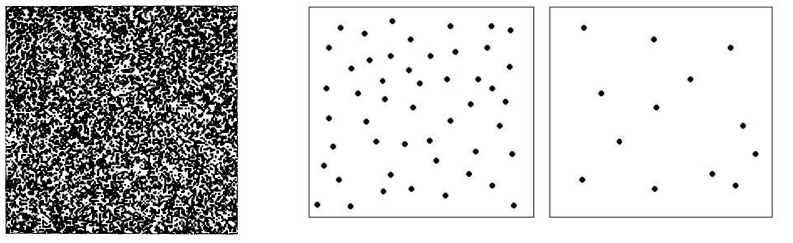
\includegraphics[width=0.6\textwidth]{helmholtz_principle}        
    \caption{Representation of the Helmholtz's principle: a) Uniform random imagen where no structure can be found. A group of five aligned dots exist in both images b) and c), but this structure can hardly be seen in the central image. Otherwise, in the right-most image the alignment stands out as an important deviation from randomness that cannot happen by chance and is therefore perceived.}\label{fig:helmholtz_principle}
\end{figure}


The Gestalt theory \citep{Wertheimer:Psycologische:1923} states that we can build a whole (gestalt) through the grouping of non-accidental detected primitives. That is, the human mind recognizes objects as a whole before examining their individual parts and the information that is not related in size, shape, orientation, etc., is perceived by the observer as chaotic and disorganized. The grouping of individual elements in a whole follows a set of laws defined by the Gestalt theory; some of them are (see Fig. \ref{fig:gestalt_laws}):

\begin{itemize}
	\item Similarity law
	\item Proximity law
	\item Continuity law
	\item Closure law
	\item Connectedness law
	\item Figure-ground law
	
\end{itemize}

\begin{figure}[!ht]
    \centering
    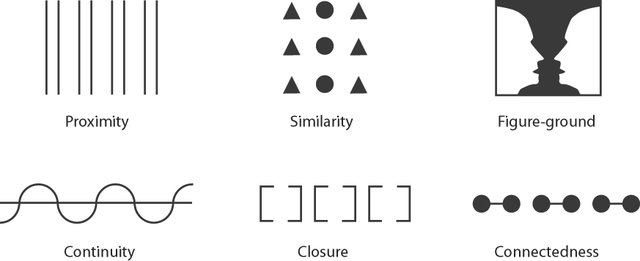
\includegraphics[width=0.6\textwidth]{gestalt_laws}        
    \caption{Graphic representation of the Gestalt's law of grouping.}\label{fig:gestalt_laws}
\end{figure}

In this work, we explore the above ideas and propose a novel approach to detect a landing target in the same way as humans do, imitating the human perception process. To achieve this, we use the image contours retrieved at different scales. From this set of contours, we obtain the most perceptual contours, that is, those that were not generated by chance using an a contrario approach. After this, we take advantage of the predefined form of the targets to propose some measures that represent the laws of grouping of similarity and proximity of the Gestalt. Finally, we do the decoding and correction of target identification errors using Hamming's code. The diagram shown in figure \ref{fig:target_detection_pipeline} groups the stages of our method for the perceptual detection of landing targets.

\begin{figure}[!ht]
    \centering
    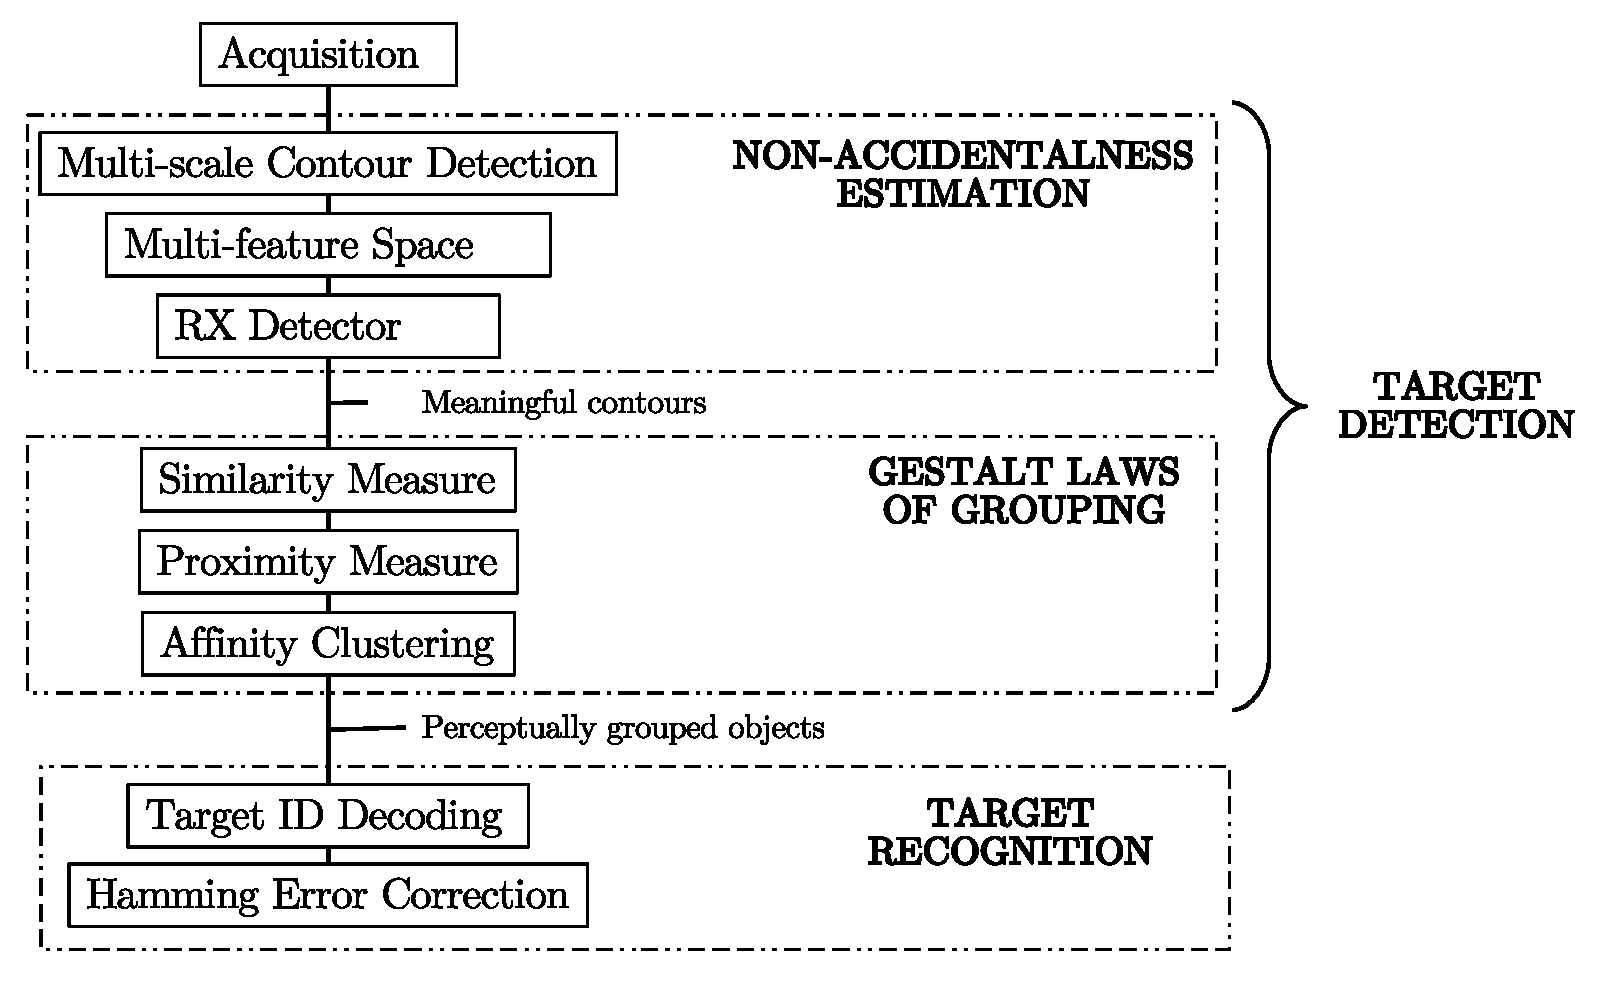
\includegraphics[width=\textwidth]{target_detection_pipeline}        
    \caption{Diagram of the phases involved in the landing target detection and recognition task.}\label{fig:target_detection_pipeline}
\end{figure}

The following sections are devoted to detailing the framework for the detection of landing targets. In section \ref{sec:hierarchical_target_detection} we evaluate different threshold-based methods for obtaining contours in an algorithm that uses the hierarchy of contours for the detection of landing targets. After that, we develop our perception model in section \ref{sec:unsupervised_perception_model}. Specifically, subsection \ref{subsec:Helmholtz} describes how to retrieve image contours as meaningful primitives and subsection \ref{subsec:Gestalt} describes how to group the contours to detect a landing target perceptually.  Later, in section \ref{sec:validation_and_test} we present the implementation of our methodology and some tests with both, synthetic and real-life images. We also present some conclusion and perspectives in section \ref{sec:conclusions_landing_target}. Finally, the appendix \ref{ch:target_description} contains the description of the landing target as well as the strategy used for its generation.


\section{Hierarchical Countours for Target Detection}\label{sec:hierarchical_target_detection}

Originally, the idea of landing targets detection is inspired by the needs of the \cite{Internest:WebPage:} company. The objective is to design a landing marker and an algorithm for its detection; all of this in the context of the UAV's autonomous precision landing task. 
A first approach, developed during the traineeship period of a master student \citep{BaquedanoA.:ESIEE:2017}, seeks to solve the task straightforwardly using highly studied techniques. The algorithm is based on finding the contours of a binary image generated by the threshold method proposed by \cite{Otsu:SMC:1979}. Since the landing target they propose is composed of nested concentric circles, they heuristically use the hierarchy of the found contours to detect a landing target. Their methodology consists in discriminating the contours that are not nested through conditional evaluations at each hierarchy level. The conditions are hierarchically dependent which means that the landing target detection is frustrated if the conditions are not strictly enforced.

This idea was tested, however, similarly to some other works mentioned in section \ref{sec:introduction_ch1}, the algorithm works well only under certain circumstances. The tests show that the algorithm fails mainly because it is not able to find all the target contours, what compromises the hierarchical condition fro detection. This generally occurs when the landing target is exposed to conditions that degrade the quality of the image. Given the nature of the aerial object detection task, factors such as the change in height and orientation of the UAV, modify the perception of an object introducing disturbances such as noise, changes in lighting and contrast, deformation of objects, etc.. Such image degrataions complicate the operation of threshold-based and consequently the contour detection. We classify the disturbances suffered by landing targets into four types: 

\begin{enumerate}
	\item Change in size w.r.t. the scene.
	\item Presence of noise.
	\item Presence of shadows.
	\item Deformation due to perspective.
\end{enumerate}
Figure \ref{fig:tar_degradations} shows a landing target affected by the aforementioned disturbances.
  
\begin{figure}[!ht]
    \centering
    \begin{subfigure}[b]{0.3\textwidth}
        \frame{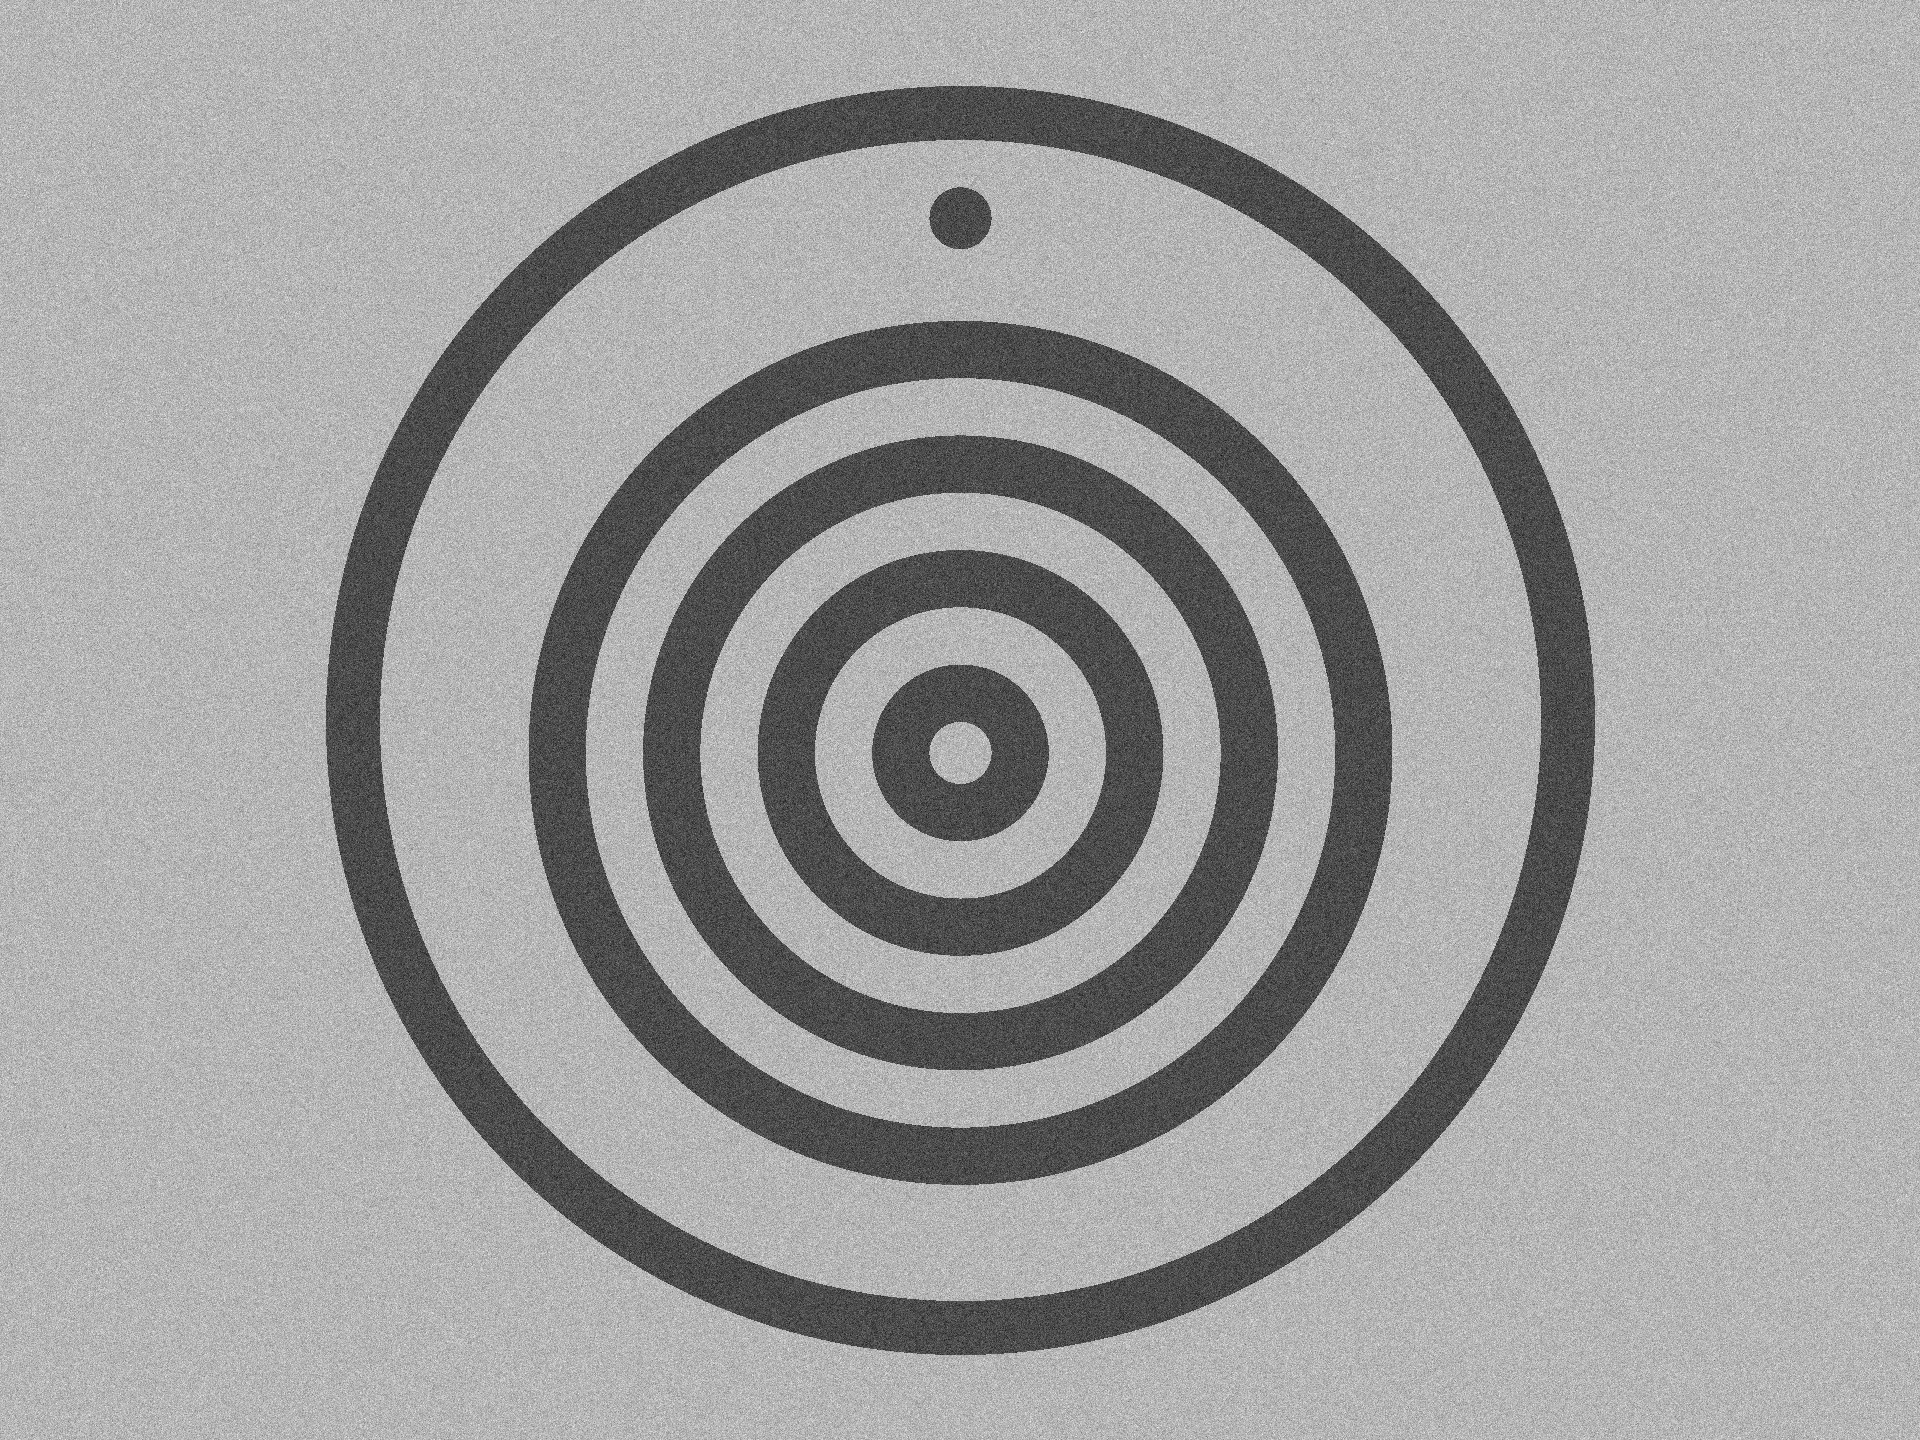
\includegraphics[width=\textwidth]{tar_noise}}
        \caption{}
        \label{fig:deg_noise}
    \end{subfigure}
        ~ %add desired spacing between images, e. g. ~, \quad, \qquad, \hfill etc. 
      %(or a blank line to force the subfigure onto a new line)
    \begin{subfigure}[b]{0.3\textwidth}
        \frame{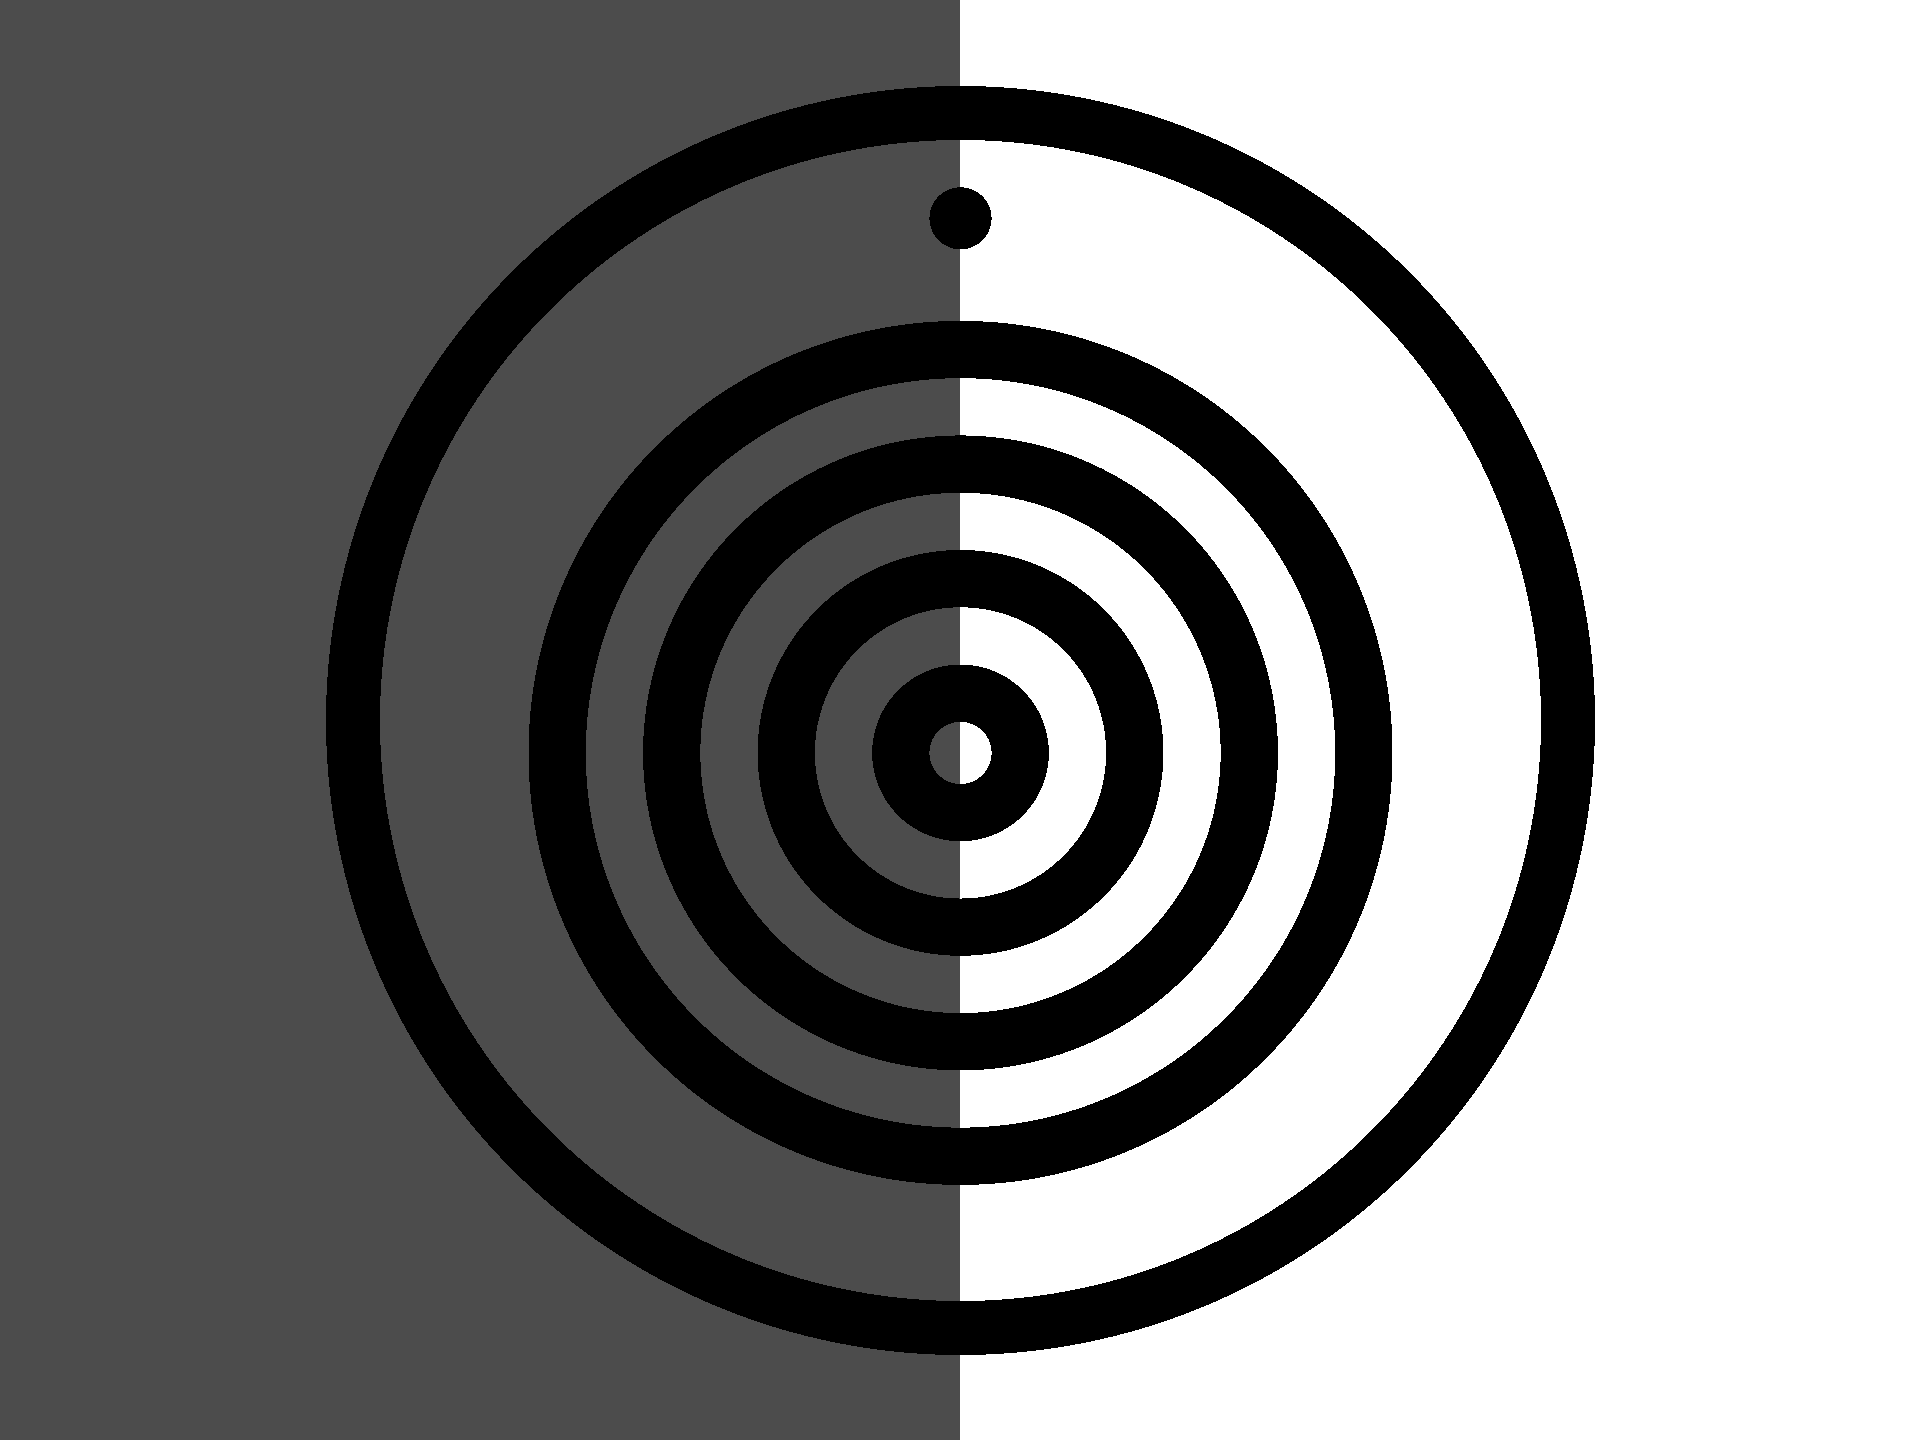
\includegraphics[width=\textwidth]{tar_shadow}}
        \caption{}
        \label{fig:deg_shadow}
    \end{subfigure}\\
        ~ %add desired spacing between images, e. g. ~, \quad, \qquad, \hfill etc. 
      %(or a blank line to force the subfigure onto a new line)
    \begin{subfigure}[b]{0.3\textwidth}
        \frame{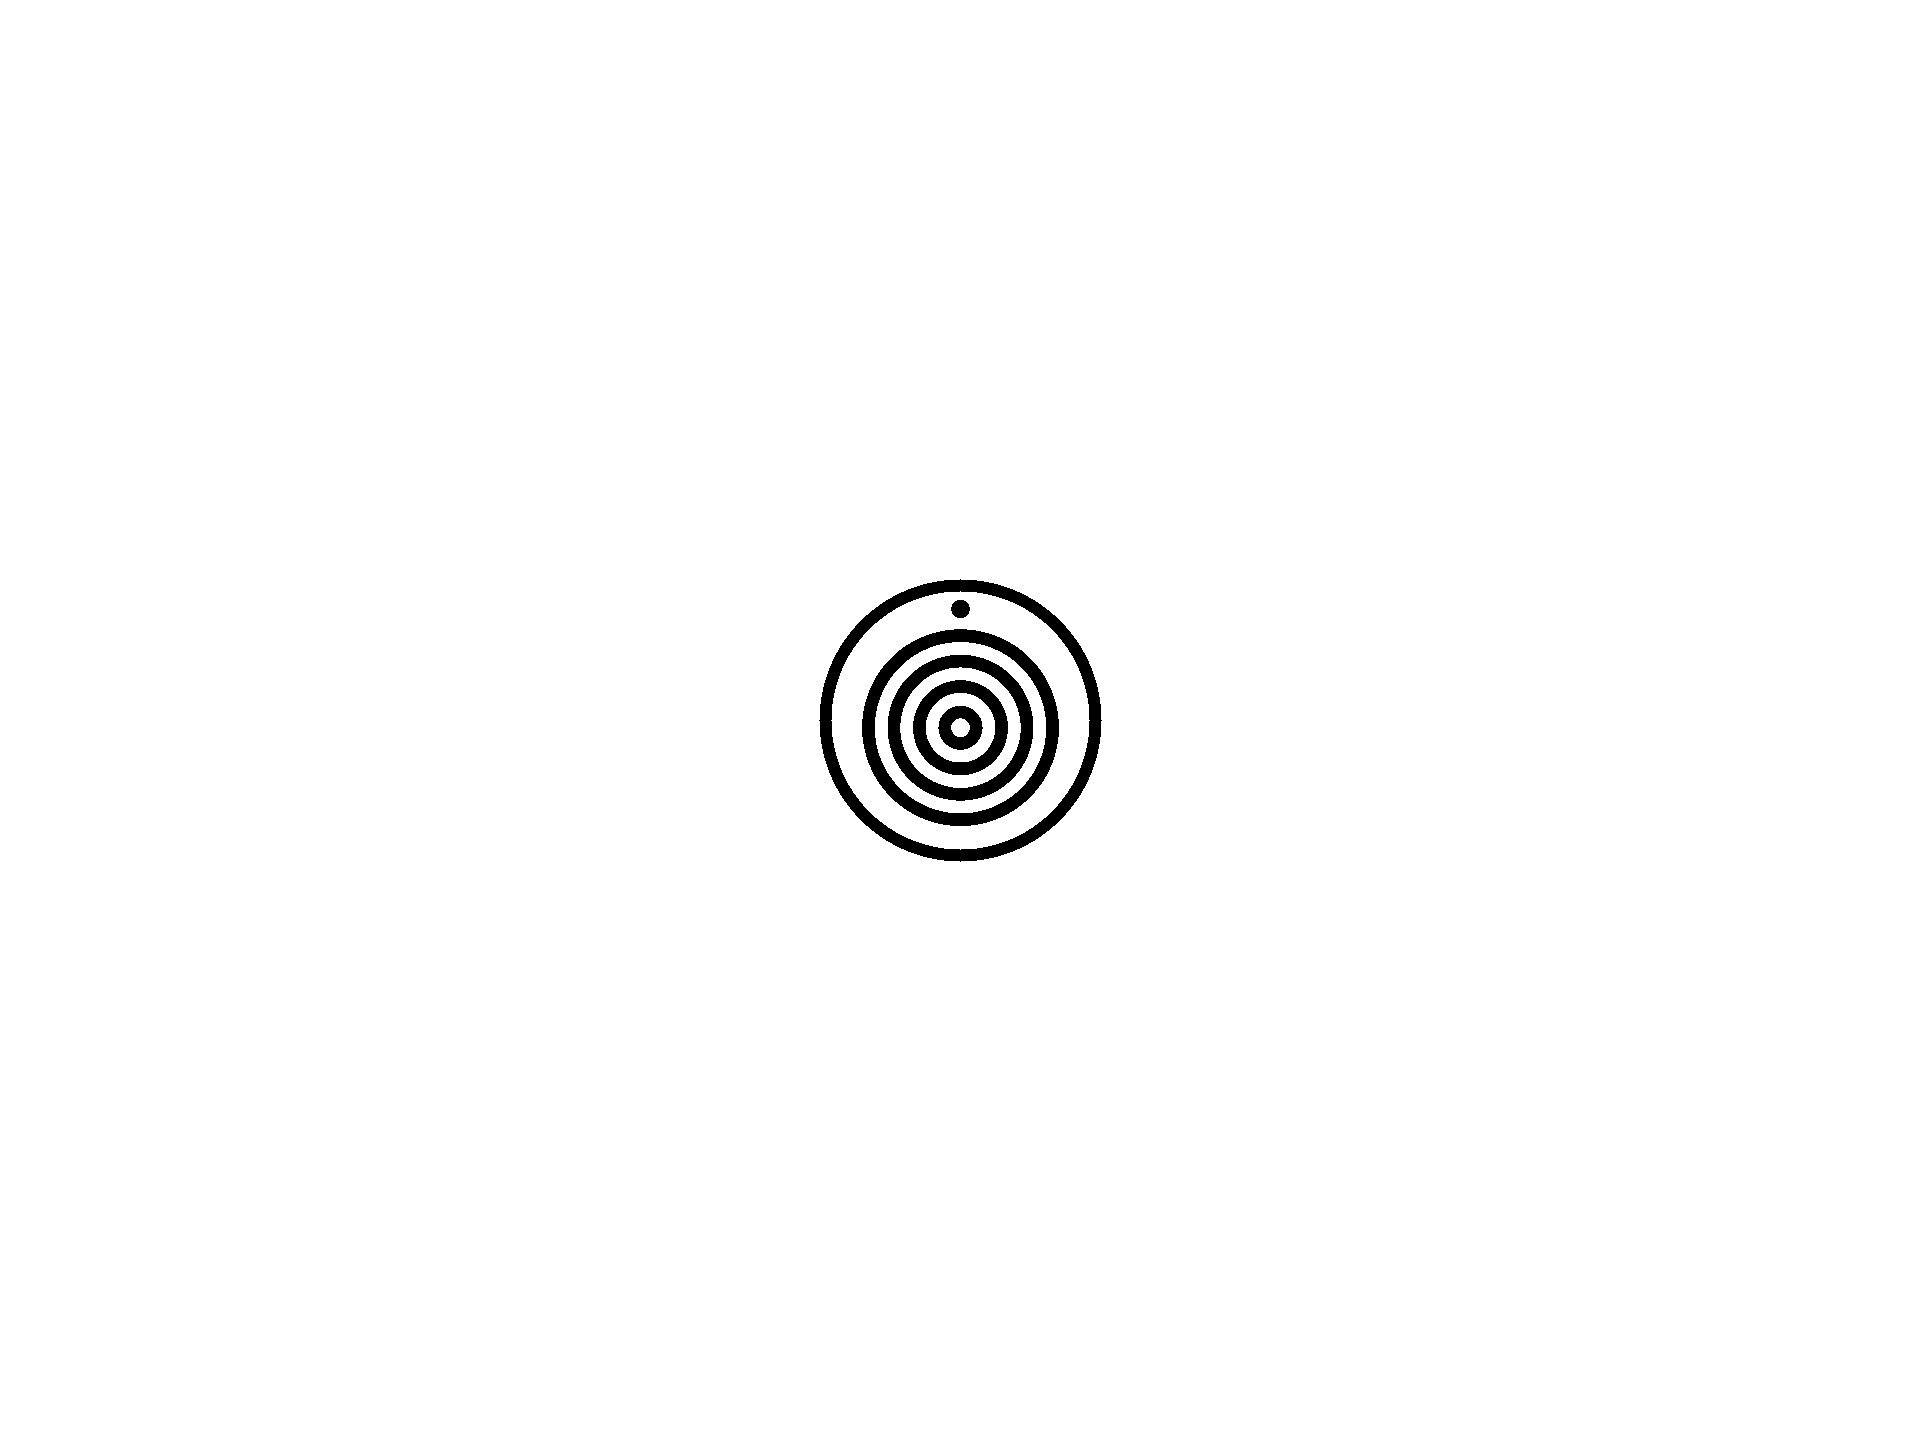
\includegraphics[width=\textwidth]{tar_resolution}}
        \caption{}
        \label{fig:deg_resolution}
    \end{subfigure}
        ~ %add desired spacing between images, e. g. ~, \quad, \qquad, \hfill etc. 
      %(or a blank line to force the subfigure onto a new line)
    \begin{subfigure}[b]{0.3\textwidth}
        \frame{
\includegraphics[width=\textwidth]{tar_deformation}}
        \caption{}
        \label{fig:deg_deformation}
    \end{subfigure}
    \caption{ Landing target degradations: \textbf{(a)} Noise, \textbf{(b)} Shadow, \textbf{(c)} Change of size and \textbf{(d)} Perspectice deformation}\label{fig:tar_degradations}
\end{figure}


One of the main disadvantages of the hierarchy method for the landing targets detection is that its effectiveness lies with the Otsu contour detector, which does not work well in images with high contrast or severe changes in lighting. However, there are other threshold-based methods for contour detection that could better face the image degradations showed in figure \ref{fig:tar_degradations}. Following the taxonomy for threshold-based methods proposed in \citep{Sezgin.Sankur:EI:2010}, there are clustering-based methods such as \cite{Otsu:SMC:1979} and \cite{Ridler.Calvard:TSMC:1978} edge detectors; entropy-based methods such as \cite{Yen.Chang.ea:TIP:1995} and \cite{Li.Lee:ICPR:1993} detectors; local methods such as \cite{Niblack:ImageProcc:1986} and \cite{Sauvola.Pietikainen:ICPR:2000} operators; the adaptive method proposed by \cite{Bradley.Roth:ACM:2007} and finally, the mean and Gaussian pixel distribution as spacial methods. 
We use these nine representative threshold-based methods to obtain a binary image, localize the image contours and evaluate which is the best approach facing the image degradations showed in figure \ref{fig:tar_degradations}.


\begin{figure}[htbp]
\centering
\begin{subfigure}[t]{\dimexpr0.15\textwidth+20pt\relax}
    \makebox[20pt]{\raisebox{30pt}{\rotatebox[origin=c]{90}{Input}}}%Input (zoom)
    \frame{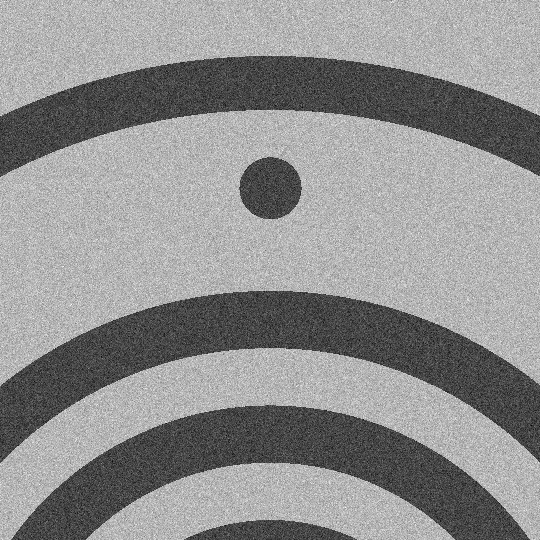
\includegraphics[width=\dimexpr\linewidth-20pt\relax]
    {tar_zoom_noise}}
    \makebox[20pt]{\raisebox{30pt}{\rotatebox[origin=c]{90}{Otsu}}}%
    \frame{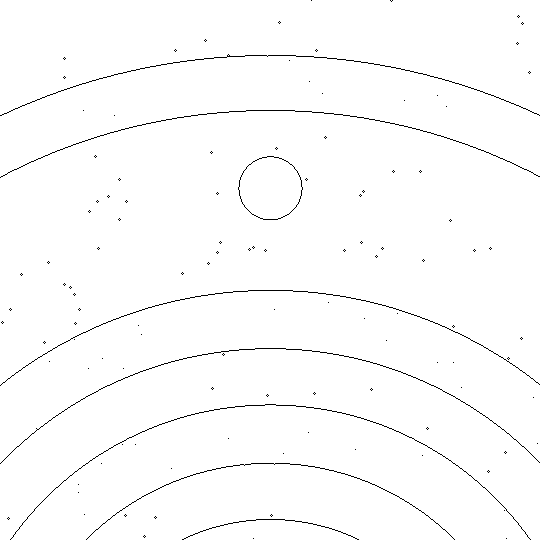
\includegraphics[width=\dimexpr\linewidth-20pt\relax]
    {Otsu_cont_noise}}
    \makebox[20pt]{\raisebox{30pt}{\rotatebox[origin=c]{90}{Riddler}}}%
    \frame{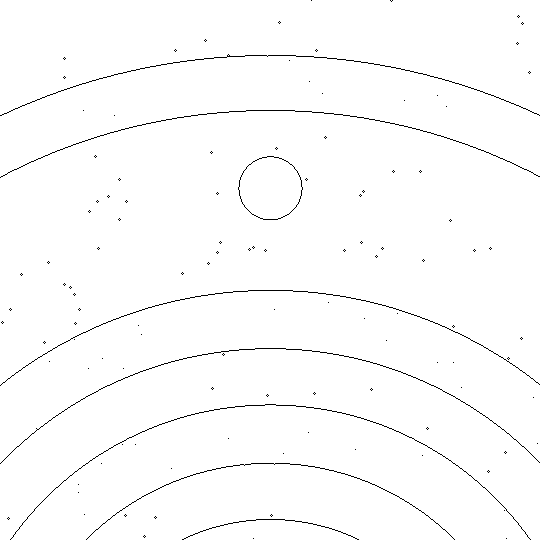
\includegraphics[width=\dimexpr\linewidth-20pt\relax]
    {Riddler_cont_noise}}
    \makebox[20pt]{\raisebox{30pt}{\rotatebox[origin=c]{90}{Yen}}}%
    \frame{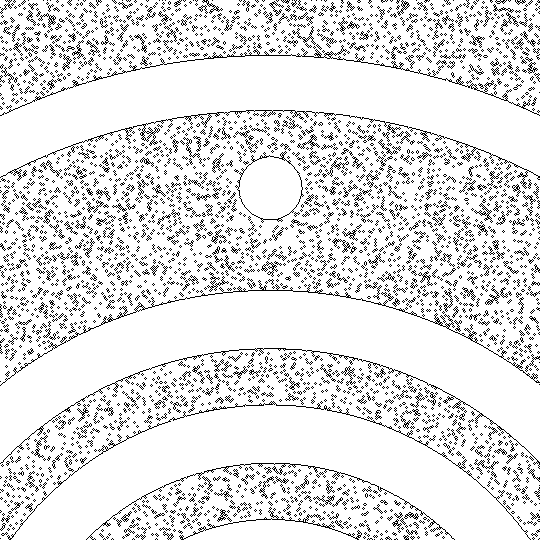
\includegraphics[width=\dimexpr\linewidth-20pt\relax]
    {Yen_cont_noise}}
    \makebox[20pt]{\raisebox{30pt}{\rotatebox[origin=c]{90}{Li}}}%
    \frame{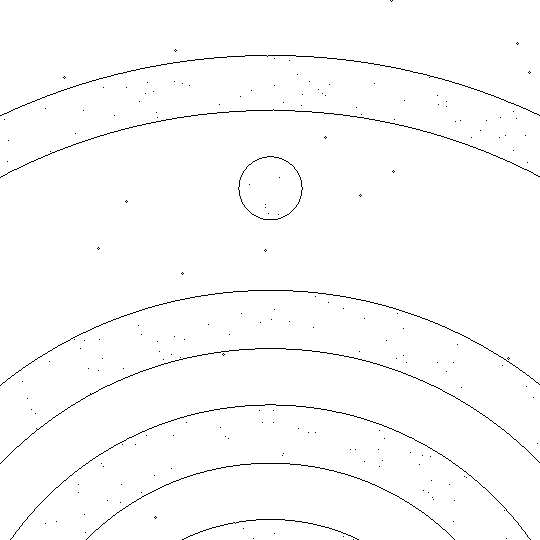
\includegraphics[width=\dimexpr\linewidth-20pt\relax]
    {Li_cont_noise}}
    \makebox[20pt]{\raisebox{30pt}{\rotatebox[origin=c]{90}{Niblack}}}%
    \frame{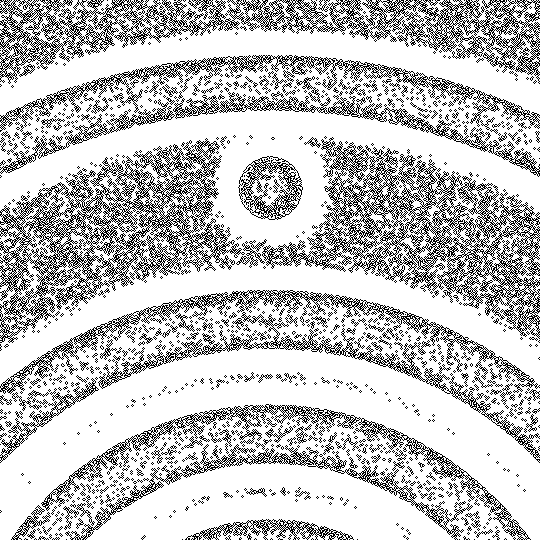
\includegraphics[width=\dimexpr\linewidth-20pt\relax]
    {Niblack_cont_noise}}
    \makebox[20pt]{\raisebox{30pt}{\rotatebox[origin=c]{90}{Sauvola}}}%
    \frame{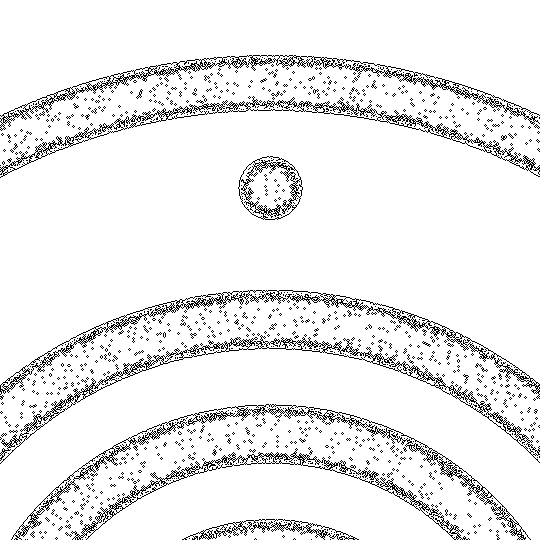
\includegraphics[width=\dimexpr\linewidth-20pt\relax]
    {Sauvola_cont_noise}}
    \makebox[20pt]{\raisebox{30pt}{\rotatebox[origin=c]{90}{Bradley}}}%
    \frame{
\includegraphics[width=\dimexpr\linewidth-20pt\relax]
    {Bradley_cont_noise}}
    \makebox[20pt]{\raisebox{30pt}{\rotatebox[origin=c]{90}{Gauss}}}%
    \frame{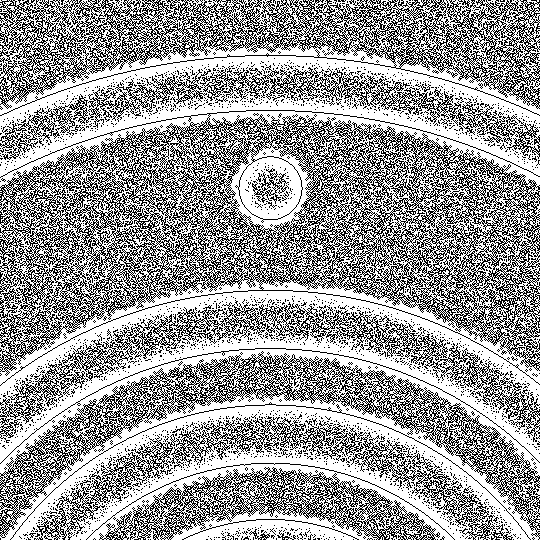
\includegraphics[width=\dimexpr\linewidth-20pt\relax]
    {Gauss_cont_noise}}
    \makebox[20pt]{\raisebox{30pt}{\rotatebox[origin=c]{90}{Mean}}}%
    \frame{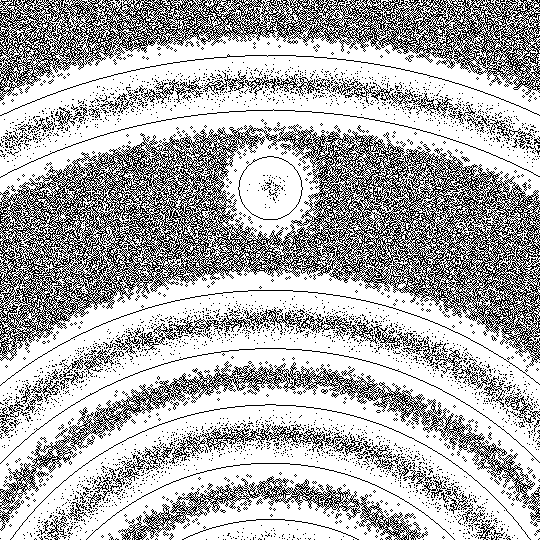
\includegraphics[width=\dimexpr\linewidth-20pt\relax]
    {Mean_cont_noise}}
    \caption{} 
\end{subfigure}\qquad
\begin{subfigure}[t]{0.15\textwidth}
    \frame{
\includegraphics[width=\textwidth]
    {tar_zoom_shadow}}
    \frame{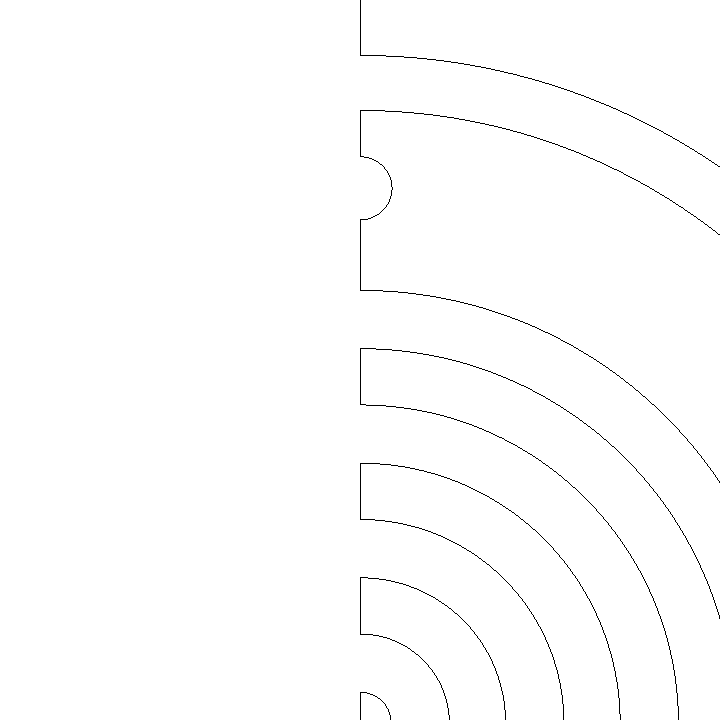
\includegraphics[width=\textwidth]
    {Otsu_cont_shadow}}
    \frame{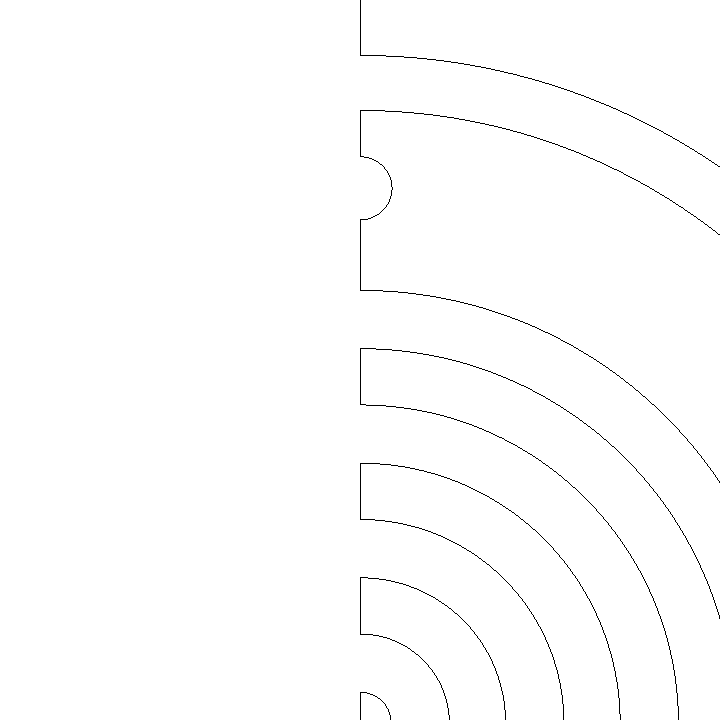
\includegraphics[width=\textwidth]
    {Riddler_cont_shadow}}
    \frame{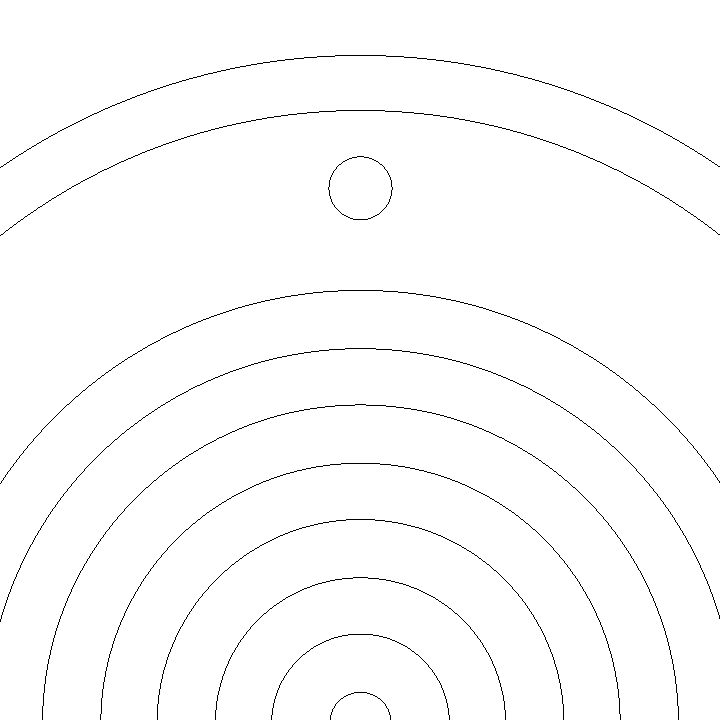
\includegraphics[width=\textwidth]
    {Yen_cont_shadow}}
    \frame{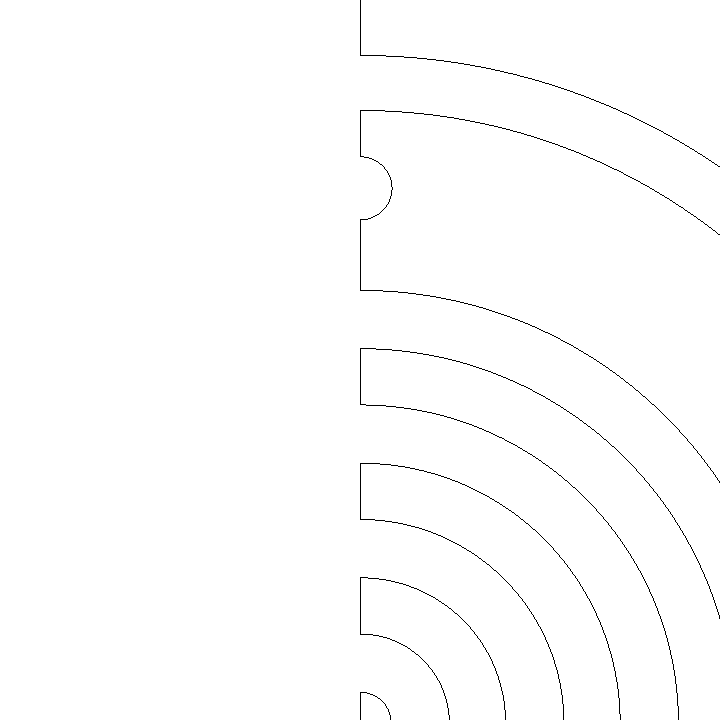
\includegraphics[width=\textwidth]
    {Li_cont_shadow}}
    \frame{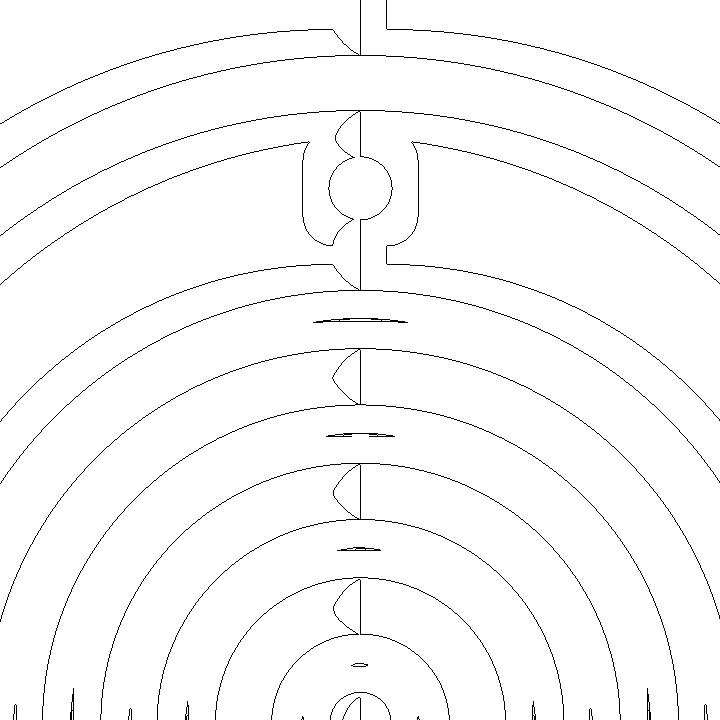
\includegraphics[width=\textwidth]
    {Niblack_cont_shadow}}
    \frame{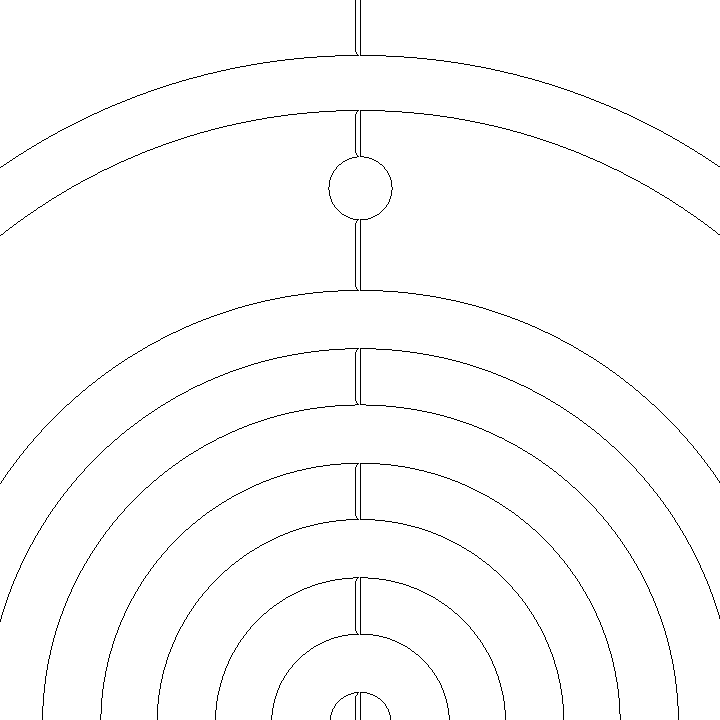
\includegraphics[width=\textwidth]
    {Sauvola_cont_shadow}}
    \frame{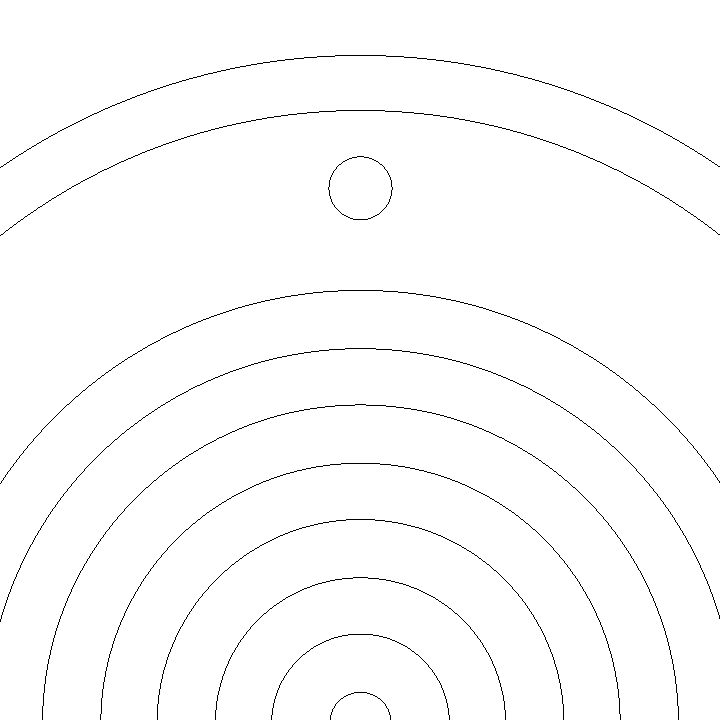
\includegraphics[width=\textwidth]
    {Bradley_cont_shadow}}
    \frame{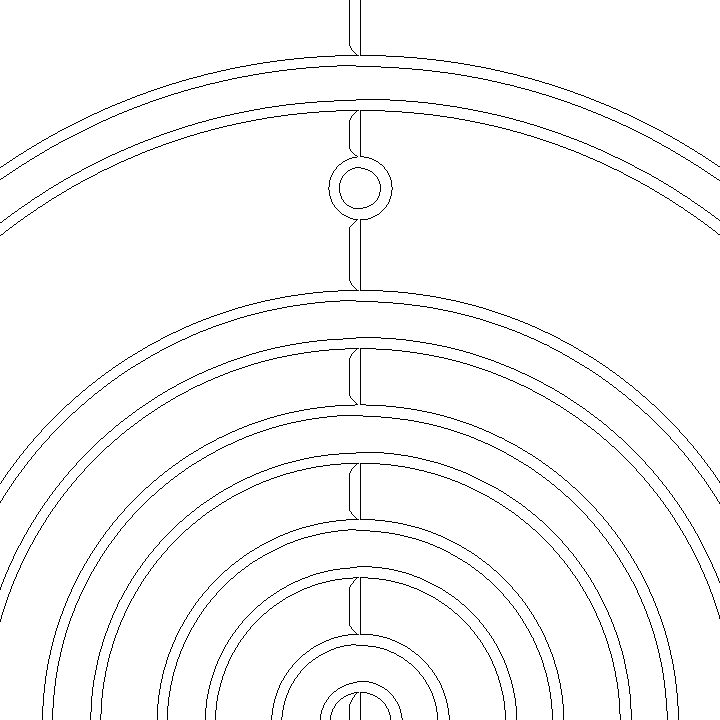
\includegraphics[width=\textwidth]
    {Gauss_cont_shadow}}
    \frame{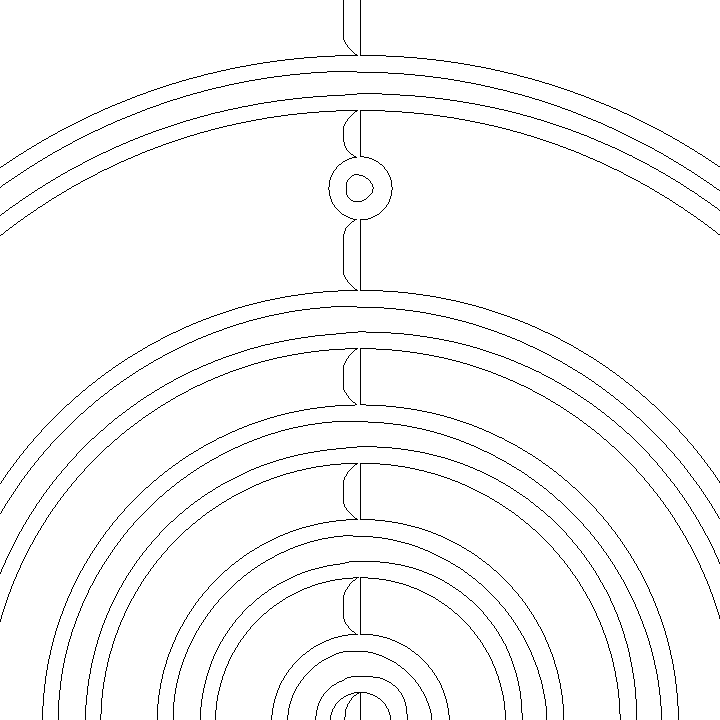
\includegraphics[width=\textwidth]
    {Mean_cont_shadow}}
    \caption{} 
\end{subfigure}\qquad
\begin{subfigure}[t]{0.15\textwidth}
    \frame{
\includegraphics[width=\textwidth]
    {tar_zoom_resolution}}
    \frame{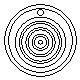
\includegraphics[width=\textwidth]
    {Otsu_cont_resolution}}
    \frame{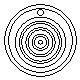
\includegraphics[width=\textwidth]
    {Riddler_cont_resolution}}
    \frame{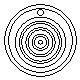
\includegraphics[width=\textwidth]
    {Yen_cont_resolution}}
    \frame{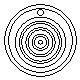
\includegraphics[width=\textwidth]
    {Li_cont_resolution}}
    \frame{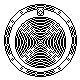
\includegraphics[width=\textwidth]
    {Niblack_cont_resolution}}
    \frame{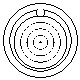
\includegraphics[width=\textwidth]
    {Sauvola_cont_resolution}}
    \frame{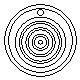
\includegraphics[width=\textwidth]
    {Bradley_cont_resolution}}
    \frame{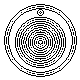
\includegraphics[width=\textwidth]
    {Gauss_cont_resolution}}
    \frame{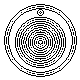
\includegraphics[width=\textwidth]
    {Mean_cont_resolution}}
    \caption{} 
\end{subfigure}\qquad
\begin{subfigure}[t]{0.15\textwidth}
    \frame{
\includegraphics[width=\textwidth]
    {tar_zoom_deformation}}
    \frame{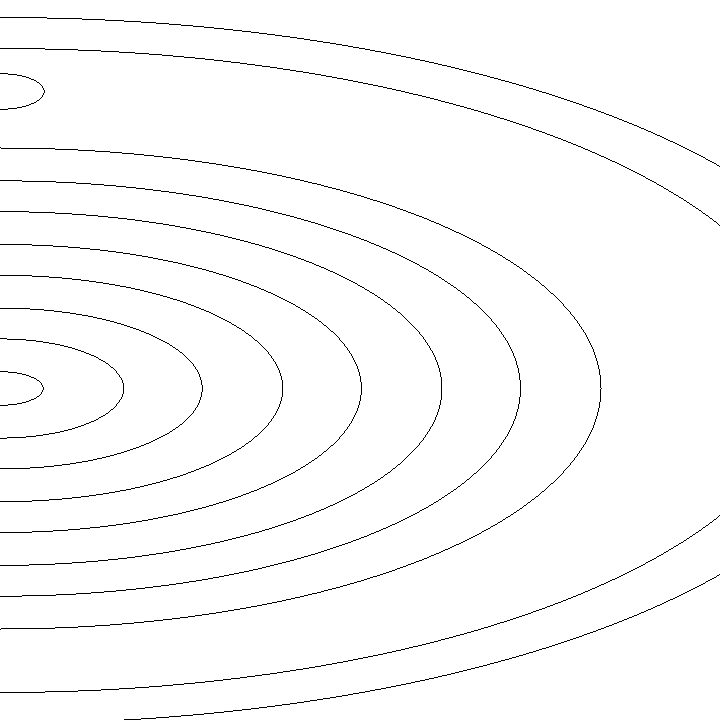
\includegraphics[width=\textwidth]
    {Otsu_cont_deformation}}
    \frame{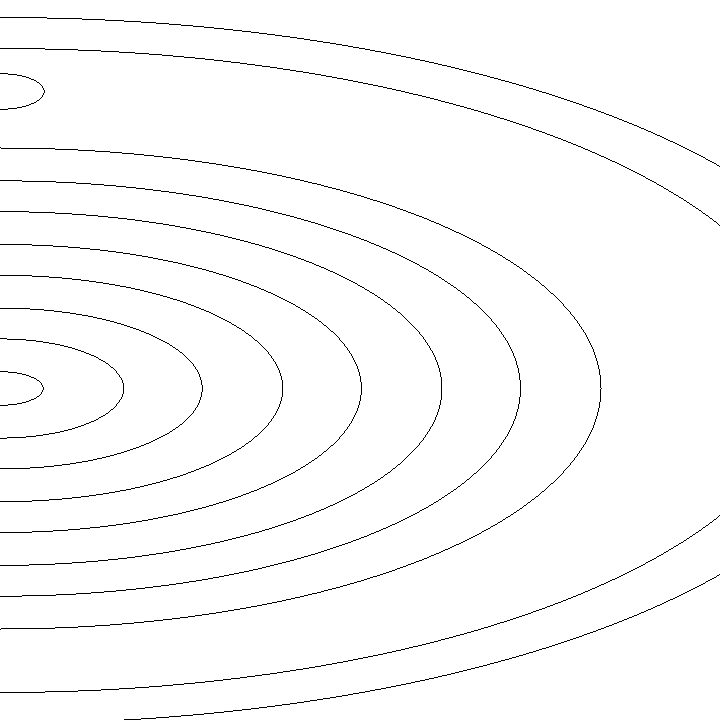
\includegraphics[width=\textwidth]
    {Riddler_cont_deformation}}
    \frame{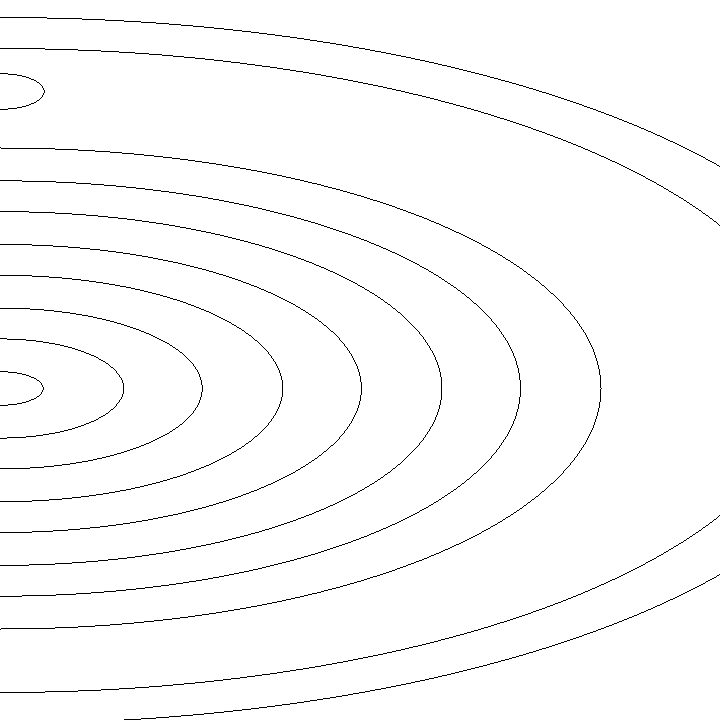
\includegraphics[width=\textwidth]
    {Yen_cont_deformation}}
    \frame{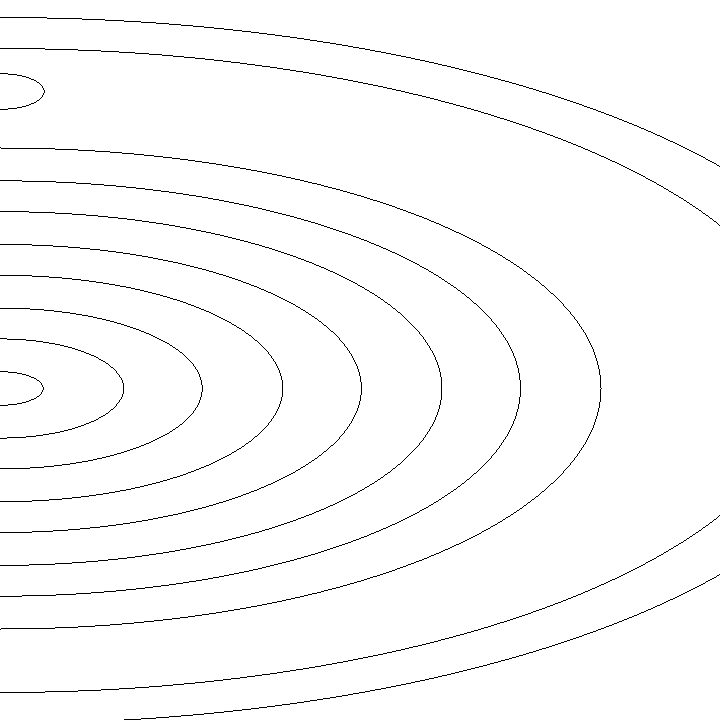
\includegraphics[width=\textwidth]
    {Li_cont_deformation}}
    \frame{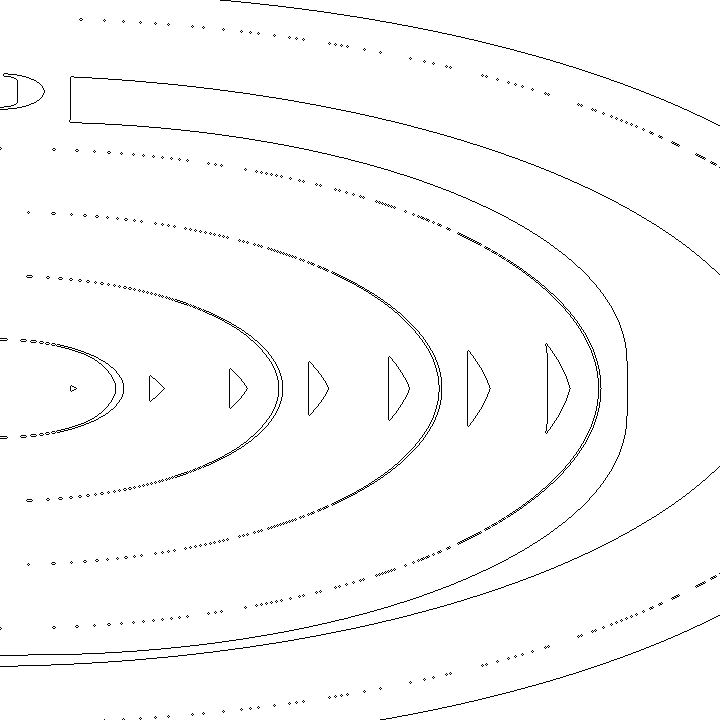
\includegraphics[width=\textwidth]
    {Niblack_cont_deformation}}
    \frame{\includegraphics[width=\textwidth]
    {Sauvola_cont_deformation}}
    \frame{\includegraphics[width=\textwidth]
    {Bradley_cont_deformation}}
    \frame{\includegraphics[width=\textwidth]
    {Gauss_cont_deformation}}
    \frame{\includegraphics[width=\textwidth]
    {Mean_cont_deformation}}
    \caption{}  
\end{subfigure}
\caption{threshold-based methods result illustrations on synthetic images: \textbf{(a)} Noise, \textbf{(b)} Shadow, \textbf{(c)} Size and \textbf{(d)} Deformation degradations}\label{fig:thr_synth_comparison}
\end{figure}

The contours obtained applying each threshold-based method are depicted in figure \ref{fig:thr_synth_comparison}. In this figure is appreciable that, depending on the situation, the result is better or worse. For example, we can see that the Otsu, Riddler, Yen and Li methods react appropriately to the target scale change, but none of these four methods except the Yen operator work correctly in the presence of shadows. This results from the comparison of four methods under two disturbances, however, of the nine methods there are none that works correctly for all perturbations.

\subsection{Thershold-based Method's Evaluation}
We run the hierarchical algorithm proposed in \citep{BaquedanoA.:ESIEE:2017} on a database of synthetic images. The database contains the sixteen different landing targets perturbed by the image degradations of figure \ref{fig:tar_degradations}. 
The noise degradation is simulated by adding a Gaussian noise with mean of zero and a standard deviation variable from 0.02 to 0.2 where 0.02 is the minimum noise addition. The shadow perturbation is simulated shading the left-half of the image; the variation of the shadow is done between 0 and 1 where 0 indicates a darker left-half image. The last two degradations are related with the perspective and distance of the viewer (the camera). First, we change the size of the landing target by scaling forming circles on a $640\times480$p image.  The range of the scale is from 0 to 1, where 1 indicates real scale. Lastly, to achieve the perspective degradation we consider that the circular target behaves like an ellipse when it is not seen from the perpendicular axis of the center. Therefore, we deform the target synthetically by augmenting the proportion of one axis (major and minor) of the ellipse in an interval between 1 and 2, where 2 indicates the maximum deformation. 

For the test of the different contour detectors, we apply the maximum value of each degradation. We use the F1-score as metric to evaluate the accuracy of each threshold-based method under the different degradations. This metric has values between 0 and 1, where 1 is the best score and 0 the worst. Figure \ref{fig:degradations_graphs} shows the performance of all nine detectors on each disturbance separately in the form of bar plots. The graphs show the F1-score of the hierarchical detection algorithm without the Hamming error-correction (gray bars) and with the use of the Hamming error-correction (black bars) described in appendix \ref{ch:target_description}.

\begin{figure}[!ht]
    \centering
    \begin{subfigure}[b]{0.4\textwidth}
        \includegraphics[width=\textwidth]{noise_comparison}
        \caption{}
        \label{fig:noise_graph}
    \end{subfigure}
        ~ %add desired spacing between images, e. g. ~, \quad, \qquad, \hfill etc. 
      %(or a blank line to force the subfigure onto a new line)
    \begin{subfigure}[b]{0.4\textwidth}
        \includegraphics[width=\textwidth]{shade_comparison}
        \caption{}
        \label{fig:shadow_graph}
    \end{subfigure}\\
        ~ %add desired spacing between images, e. g. ~, \quad, \qquad, \hfill etc. 
      %(or a blank line to force the subfigure onto a new line)
    \begin{subfigure}[b]{0.4\textwidth}
        \includegraphics[width=\textwidth]{resolution_comparison}
        \caption{}
        \label{fig:resolution_graph}
    \end{subfigure}
        ~ %add desired spacing between images, e. g. ~, \quad, \qquad, \hfill etc. 
      %(or a blank line to force the subfigure onto a new line)
    \begin{subfigure}[b]{0.4\textwidth}
        \includegraphics[width=\textwidth]{ellipse_comparison}
        \caption{}
        \label{fig:deformation_graph}
    \end{subfigure}
    \caption{F1-score bar graphs: \textbf{(a)} Noise, \textbf{(b)} Shadow, \textbf{(c)} Change of size and \textbf{(d)} Perspectice deformation}\label{fig:degradations_graphs}
\end{figure}

Although the experiments use the highest values of target deformation, they do not consider the combination of two or more degradations, which is closer to reality. Figure \ref{fig:input_image} shows one of our targets (target ID 4) under real lighting conditions, i.e., in an outdoor environment where the four degradations of the experiment are present. We also show his histogram to highlight the saturation levels of the scene and the contours obtained with a representative method of each class of the taxonomy in \citep{Sezgin.Sankur:EI:2010}: clustering-based (Fig. \ref{fig:otsu_th}), entropy-based (Fig. \ref{fig:li_th}), spacial (Fig. \ref{fig:gauss_th}) and local (Fig. \ref{fig:sauvola_th}) threshold-based methods. 

\begin{figure}[!ht]
    \centering
    \begin{subfigure}[b]{0.3\textwidth}
        \frame{\includegraphics[width=\textwidth]{in_img_tar4}}
        \caption{Input image}
        \label{fig:input_image}
    \end{subfigure}
    ~ %add desired spacing between images, e. g. ~, \quad, \qquad, \hfill etc. 
      %(or a blank line to force the subfigure onto a new line)
    \begin{subfigure}[b]{0.3\textwidth}
        \includegraphics[width=\textwidth]{histogram}
        \caption{Histogram of input image}
        \label{fig:histogram}
    \end{subfigure}\\
        ~ %add desired spacing between images, e. g. ~, \quad, \qquad, \hfill etc. 
      %(or a blank line to force the subfigure onto a new line)
    \begin{subfigure}[b]{0.16\textwidth}
        \frame{\includegraphics[width=\textwidth]{in_img_tar4_zoom}}
        \caption{Zoom}
        \label{fig:tar4_zoom}
    \end{subfigure}
        ~ %add desired spacing between images, e. g. ~, \quad, \qquad, \hfill etc. 
      %(or a blank line to force the subfigure onto a new line)
    \begin{subfigure}[b]{0.16\textwidth}
        \frame{\includegraphics[width=\textwidth]{Otsu_cont}}
        \caption{Otsu}
        \label{fig:otsu_th}
    \end{subfigure}
        ~ %add desired spacing between images, e. g. ~, \quad, \qquad, \hfill etc. 
      %(or a blank line to force the subfigure onto a new line)
    \begin{subfigure}[b]{0.16\textwidth}
        \frame{\includegraphics[width=\textwidth]{Li_cont}}
        \caption{Li}
        \label{fig:li_th}
    \end{subfigure}
        ~ %add desired spacing between images, e. g. ~, \quad, \qquad, \hfill etc. 
      %(or a blank line to force the subfigure onto a new line)
    \begin{subfigure}[b]{0.16\textwidth}
        \frame{\includegraphics[width=\textwidth]{Gauss_cont}}
        \caption{Gauss }
        \label{fig:gauss_th}
    \end{subfigure}
        ~ %add desired spacing between images, e. g. ~, \quad, \qquad, \hfill etc. 
      %(or a blank line to force the subfigure onto a new line)
    \begin{subfigure}[b]{0.16\textwidth}
        \frame{\includegraphics[width=\textwidth]{Sauvola_cont}}
        \caption{Sauvola}
        \label{fig:sauvola_th}
    \end{subfigure}
    \caption{Landing target under non-controlled illumination conditions and the controus obtained with some threshold-based methods}\label{fig:thresholding_comp}
\end{figure}

The F1-score bar plots (figure \ref{fig:degradations_graphs}) and figure \ref{fig:thresholding_comp} show that given the conditions where a landing target can be found, no threshold-based method was robust to the set of perturbations. It is necessary to adjust parameters according to the condition to have acceptable results. Besides, we aim to recognize the landing targets in natural images where none, one or more landing targets can be present and the degradations are not isolated. 

\section{Unsupervised Perception Model}\label{sec:unsupervised_perception_model}
%
\subsection{Non-accidentalness Estimation}\label{subsec:Helmholtz}

\subsubsection{Contour Detection}\label{subsubsec:muiltiscale}

After the development of a first algorithm by \citep{BaquedanoA.:ESIEE:2017}, we take some elements of this work to develop a more general approach that explores the principles of human perception. Precisely, we keep the concept of concentric circle patterns for the generation of landing target (see appendix \ref{ch:target_description} for the description of the landing targets generation) and the use of images contours as input data.

Instead of using a threshold-based method, we obtain the image without fixing any parameter using the \cite{Marr.Hildreth:PRS:1980} operator. The use of the Marr-Hildreth operator guarantees to find continuous and closed contours eliminating the possible noise in the image, while the contours of objects remain unchanged in the presence of shadows. This technique convolves the intensity image $f$ with the 2-d Laplacian of Gaussian (LoG) operator $\nabla^{2} G(x, y,\sigma)$ and generates an image, 
\begin{eqnarray}\label{eq:LoG}
l_\sigma =  \nabla^{2} G(\sigma)\ast f
\end{eqnarray}
in which we localize the zero-crossings. Such zero-crossings define the contours of the image.

The parameter $\sigma$ in eq. \eqref{eq:LoG} permits to control the amount of image smoothing, but also acts as scale parameter, that when varies, it generates different scale-space images. Since no single filter can be optimal simultaneously at all scales \citep{Marr.Hildreth:PRS:1980}, we use a multi-scale analysis \citep{Witkin:ICASSP:1984} to detect the zero-crossings in $l_\sigma$ at different scale-spaces to minimize the risk that some contour of interest is not detected. The image $l_\sigma$ from eq. \eqref{eq:LoG} contains a set of contours $\mathcal{L}_{\sigma}=\{L_{i}^{\sigma}, \enspace i=0, 1, \ldots, N\}$ for a given scale $\sigma$. Then, 
\begin{eqnarray}\label{eq:all_ctns_set}
\mathcal{L}=\bigcup\limits_{\sigma}  L_{\sigma}
\end{eqnarray}
represents all the contours of an image obtained at different scale-spaces. Figure \ref{fig:all_cnts} shows the set of contours $\mathcal{L}$ found for $\sigma=[1,2,3]$. We can also appreciate in the figure that at a fine scale (see figur \ref{fig:cnts_scale1}) we can observe more characteristics of the objects, i.e., there are more contours. Conversely, in coarse scales (see figure \ref{fig:cnts_scale3}), due to the smoothing, there is a spatial distortion, and fewer contours appear. However, those contours that had already appeared at a coarse scale, will not disappear. Then, exist the probability that those contours that spatially coincide on two or more scales belong to a change of intensity generated by the border of an object. 

\begin{figure}[!ht]
    \centering
    \begin{subfigure}[b]{0.3\textwidth}
        \frame{\includegraphics[width=\textwidth]{cnts_sig1_tar4}}
        \caption{$\mathcal{L}_{\sigma}$ for $\sigma=1$}
        \label{fig:cnts_scale1}
    \end{subfigure}
    ~ %add desired spacing between images, e. g. ~, \quad, \qquad, \hfill etc. 
      %(or a blank line to force the subfigure onto a new line)
    \begin{subfigure}[b]{0.3\textwidth}
        \frame{\includegraphics[width=\textwidth]{cnts_sig3_tar4}}
        \caption{$\mathcal{L}_{\sigma}$ for $\sigma=2$}
        \label{fig:cnts_scale2}
    \end{subfigure}\\
        ~ %add desired spacing between images, e. g. ~, \quad, \qquad, \hfill etc. 
      %(or a blank line to force the subfigure onto a new line)
    \begin{subfigure}[b]{0.3\textwidth}
        \frame{\includegraphics[width=\textwidth]{cnts_sig3_tar4}}
        \caption{$\mathcal{L}_{\sigma}$ for $\sigma=3$}
        \label{fig:cnts_scale3}
    \end{subfigure}
        ~ %add desired spacing between images, e. g. ~, \quad, \qquad, \hfill etc. 
      %(or a blank line to force the subfigure onto a new line)
    \begin{subfigure}[b]{0.3\textwidth}
        \frame{\includegraphics[width=\textwidth]{all_cnts_tar4}}
        \caption{Set $\mathcal{L}$ for $\sigma=[1, 2 ,3]$}
        \label{fig:all_cnts}
    \end{subfigure}
    \caption{The image contours found at three different scales joined in the set $\mathcal{L}$}\label{fig:multiscale_cnts}
\end{figure}

\subsubsection{Multi-feature Space}\label{subsec:multispace}
The Helmholtz principle states that meaningful characteristics appear as large deviations from randomness and that is how the human perception automatically works to identify an object \citep{Attneave:PR:1954}. The a contrario model proposed in \citep{Desolneux.Moisan.ea:Gestalt:2008}, formulates this principle statistically by setting the number of false alarms (NFA) below some acceptable level; however, this method cannot be easily extended to more complex shapes. Instead of setting the NFA, we use the RX detector \citep{Reed.Yu:TASSP:1990} to detect outliers. The RX anomaly detector, initially called the Constant False Alarms Rate (CFAR) detection algorithm, can detect the presence of a know signal pattern in several signal-plus-noise channels. For that, it uses a $N\times Q$ multi-variable space $Z=[Z_{1}, \ldots, Z_{Q}]$ with $Q$  observation vectors of dimension $N$. In our approach, the primitive is a closed contour. We build the multi-variable space with observations based on internal (geometrical features, e.g., circularity, roundness, area, perimeter) and external (e.g., mean gradient intensity,  intensity inner area) properties of the contours.

Let $L_{i} \in \mathcal{L}$ be a contour, $A_{i}$ its area and $P_{i}$ its perimeter; we compute the circularity eq. \eqref{eq:circuarity} and the mean gradient intensity eq. \eqref{eq:mean_gradient} to build the multi-variable space $Z=[Z_{1}, Z_{2}]$. 

\begin{eqnarray}
Z_{1}&=&\left[\frac{4\pi A_{i}}{P_{i}^2}, \enspace i=0, \ldots, N\right]^T,  \enspace N = card(\mathcal{L}) \label{eq:circuarity}  \\ 
Z_{2}&=&\left[\frac{1}{P_{i}}\sum\limits_{x \in L_{i}} \mid\nabla f(x) \mid, \enspace L_{i} \in \mathcal{L}\right]^T  \label{eq:mean_gradient}
\end{eqnarray}

\subsubsection{RX Detector}\label{subsec:rx_detector}
The RX anomaly detector \citep{Reed.Yu:TASSP:1990} is commonly used to detect outliers on such data. The space $Z$ models the set of contours $\mathcal{L}$ with $Q=2$ feature vectors describing the circularity eq. \eqref{eq:circuarity} and the mean gradient intensity eq. \eqref{eq:mean_gradient}. The RX detector gives an anomaly score to each contour taking into account the mean of the distribution and covariance between the $Q$-features through the Mahalanobis distance,
\begin{eqnarray}\label{eq:RX_detector}
y_{i}= (z_{i}-\mu_{Z})^{T}\Sigma^{-1}_{Z}(z_{i}-\mu_{Z})
\end{eqnarray}
where $\mu_{Z}=[\mathrm{E}[z_{1}], \ldots, \mathrm{E}[z_{N}]]^T$ is the meaans' observations' vector and $\Sigma^{-1}_{Z}$ the $N\times Q$ covariance matrix of the data. If the data have normal random distribution, then the score vector $Y=[y_{i}, \ldots, y_{N}]$ follows a chi-square distribution $\chi^{2}_{Q}(\varphi)$ with $Q$ degrees of freedom, where $\varphi$ is a confidence level \citep{Lu.Chen.ea:IJAIT:2004}. The value of $\chi^{2}_{Q}(\varphi)$ with a confidence value $\varphi=99.9\%$ operates as a threshold to identify all contours that behave as outliers in the multi-variable distribution. In our case, the contours belonging to a landing target appear as outliers in the vast majority of random contours belonging to the background.

With the previous strategy we preserve the anomalous contours having a value of mean gradient and circularity deviating from the principal mode of the distribution in the set $\widetilde{\mathcal{L}}=\{L_{i}\mid y_{i}>\chi^{2}_{Q}(\varphi)\}$. $\chi^{2}_{Q}(\varphi)$ is the value of the cumulative distribution at the confidence level $\varphi$ and $\widetilde{\mathcal{L}} \subset \mathcal{L}$. At this point, it is essential to mention the importance of multi-scale contour detection of section \ref{subsec:multispace}; because it increases the number of samples in $Z$, allowing to build a richer multi-variable space.

In the set $\widetilde{\mathcal{L}}$, some contours make not part of a landing target. For example, in the figure \ref{fig:rx_cnts}, we can see that the paper sheet contours remain because they have a high value of circularity. The same occurs with the contours of those objects with an important value of mean gradient, as the number 4 at the top-left of the sheet, which indicates the ID of our target, or the rock textures of the background.

\begin{figure}[!ht]
    \centering
    \frame{\includegraphics[width=0.55\linewidth]{rx_cnts_tar4}}
    \caption{The contours from Fig. \ref{fig:all_cnts} that behave as outliers in the multi-feature space $Z$ with a confidence value of $\varphi=99.9\%$}
    \label{fig:rx_cnts}
\end{figure}

\subsection{Gestalt Laws of Grouping}\label{subsec:Gestalt}
We use the Gestalt theory \citep{Wertheimer:Psycologische:1923} to group the meaningful contours $L_{i}\in \widetilde{\mathcal{L}}$ and detect landing targets.

\subsubsection{Goodness of Shape}\label{subsec:similarity}
Since the landing targets have only circular contours, we evaluate the resemblance with an ellipse (to deal with the perspective deformation) of all contours. Considering an ellipse $e_{i}$ that fits one gray contour $L_{i}$ in figure \ref{fig:affinity}, we recover the centroid $C_{i}$, the rotational angle $\rho$, the semi-major axis $\alpha_i$, the semi-minor axis $\beta_{i}$ and the coordinates $F_{i}$ and $F_{i}'$ of the ellipse's foci. Then, the sum of the distances from any point of ellipse $x_{j}\in e_{i}$ to the foci is $\overline{x_{j}F_{i}}+\overline{x_{j}F_{i}'}=2\alpha_{i}$. If the contour $L_{i}$ is an ellipse, the value $d_{i}=\abs{(\overline{x_{j}F_{i}}+\overline{x_{j}F_{i}'})-2\alpha_{i} }$ must be zero or negligible $\forall x_{j}\in L_{i}$. 

\begin{figure}[h]
    \centering
    \begin{subfigure}[b]{0.4\textwidth}
        \includegraphics[width=\textwidth]{affinity_ellipse}
        \caption{Affinity of a fit $\omega_{i}$}
        \label{fig:affinity}
    \end{subfigure}
    ~ %add desired spacing between images, e. g. ~, \quad, \qquad, \hfill etc. 
      %(or a blank line to force the subfigure onto a new line)
    \begin{subfigure}[b]{0.45\textwidth}
        \includegraphics[width=\textwidth]{DoA_ellipse}
        \caption{Difference of area $\Delta_{A_{i}}$}
        \label{fig:DoA}
    \end{subfigure}\\
    \caption{Visual description of affinity of ellipse and difference of area}\label{fig:ressemblance_ellipse}
\end{figure}

Based on the form of the landing target we estimate the the similarity using two measures, 
\begin{eqnarray}
\omega_{i}&=&\exp^{-\frac{d_{i}^{2}}{2\sigma^{2}}}\enspace \mbox{the affinity of the fit and,}\label{eq:GoE}\\
\Delta_{A_{i}}&=& 1-\frac{\abs{ A_{e_{i}}-A_{i}}}{\max(A_{e_{i}},A_{i})} \enspace \mbox{the difference of area.}\label{eq:DoA}
\end{eqnarray}

The affinity $\omega_{i}\rightarrow 1$ for contours closed to an ellipsoidal shape. However, if the contour $L_{i}$ is a croissant shape (as in fig. \ref{fig:DoA}) then, the eq. \eqref{eq:GoE} also has a high value (near to 1) but the contour is from being an ellipse. The variable in eq. \eqref{eq:DoA} complements the affinity $\omega_{i}$ taking into account the area of the ellipse $A_{e_{i}}$ and the area of the contour $A_{i}$. To calculate the similarity to an ellipse, we use the harmonic mean of both. 
\begin{eqnarray}
\kappa_{i}&=&\mathcal{H}(\omega_{i}, \Delta_{A_{i}}), \enspace \kappa_{i}\in (0,1)\label{eq:similarity}
\end{eqnarray}
where $\kappa_{i}\rightarrow 1$ for contours ressembling to an ellipse and $\kappa_{i}\rightarrow 0$ otherwise. $\mathcal{H}$ denotes the harmonic mean $\mathcal{H}= N \left(\sum\limits_{i=1}^{N} \xi_{i}^{-1} \right)^{-1}$.

\subsubsection{Proximity Measure}\label{subsec:proximity}
The Gestalt law of proximity states that we group those meaningful elements if they are spatially close to each other. In the case of contours, we take the coordinates of their centers $C_{i}$ to measure their spatial proximity.

\subsubsection{Affinity Clustering}\label{subsec:clustering}
The normalized coordinates of the centroid $C_i$ and the ellipse similarity $\kappa_i$ map the contour $L_i\in \widetilde{\mathcal{L}}$ into the 3-D space $(0,1) \in \mathbb{R}^3$. We use the affinity propagation clustering method \citep{Frey.Dueck:SCIENCE:2017} to group the contours using the matrix $X=[C_{i}, \kappa_{i}]$. This technique yields a set of clusters $\mathcal{C}_{K}\in \mathcal{C}(X)$. Because the landing target has ten different contours (see apendix \ref{ch:target_description}), the clusters with $card(\mathcal{C}_{K})\geq 10$ and an important similarity value $\mathcal{H}(\kappa_{i})\geq 0.8$, represent the candidate contours of a landing target.

\begin{figure}[h]
    \centering
    \begin{subfigure}[b]{0.3\textwidth}
        \includegraphics[width=\textwidth]{3dplot_tar4}
        \caption{Clusters obtained by affinity propagation}
        \label{fig:3dplot}
    \end{subfigure}
    ~ %add desired spacing between images, e. g. ~, \quad, \qquad, \hfill etc. 
      %(or a blank line to force the subfigure onto a new line)
    \begin{subfigure}[b]{0.3\textwidth}
        \includegraphics[width=\textwidth]{2dplot_xy_tar4}
        \caption{ Clusters projected on the image domain}
        \label{fig:2dplot}
    \end{subfigure}
    ~ %add desired spacing between images, e. g. ~, \quad, \qquad, \hfill etc. 
      %(or a blank line to force the subfigure onto a new line)
    \begin{subfigure}[b]{0.3\textwidth}
        \includegraphics[width=\textwidth]{2dplot_candidate_tar4}
        \caption{Target candidate cluster}
        \label{fig:candidate}
    \end{subfigure}
   \caption{Clusters of contour from Fig. \ref{fig:rx_cnts}}\label{fig:grouping_process}
\end{figure}

The affinity propagation technique groups in $K=12$ clusters the image contours from figure \ref{fig:rx_cnts}. In a 3D plot (fig. \ref{fig:3dplot}), we see the influence of $\kappa_{i}$ at clustering process. Projecting the clusters in a 2-D plane (fig. \ref{fig:2dplot}), we notice that even if the contours are nearby, it can form a new cluster if there is a distant $\kappa$. A clear example is the clusters 0 and 4 (blue and purple, respectively) that correspond to the contour centers of the landing target and the center of the sheet of paper, they are close to each other but the similarity not. Applying the threshold values $card(\mathcal{C}_{K})\geq 10$ and $\mathcal{H}(\kappa_{i})\geq 0.8$ we obtain the candidate clusters to form a landing target (see fig.~\ref{fig:candidate}). 

Heretofore, we have built a model based on perceptual characteristics for the landing target detection. However, there could be false detections if there are round objects with concentric borders in the image. We code an ID number in the target design to differentiate a landing target from an object with concentric circular edges. The coding of information allows discriminating between several landing targets and circular objects. The following section describes the landing target design as well as the coding and decoding technique. 

\section{Model Vadilation and Test}\label{sec:validation_and_test}
The presented strategy was validated on landing target images under simulated and real situations. We tested the algorithm in a synthetic image database which simulates four image degradations: noise, shadows, target deformation and change of size. For the real situations, we carried out several tests in indoor and outdoor scenarios. Figure \ref{fig:validation} shows three interesting experiments and the output image of each stage of section \ref{sec:perception_model}. 

\begin{figure}[h!]
\centering
\begin{subfigure}[t]{\dimexpr0.30\textwidth+20pt\relax}
    \makebox[20pt]{\raisebox{40pt}{\rotatebox[origin=c]{90}{Set $\mathcal{L}$}}}%
    \frame{\includegraphics[width=\dimexpr\linewidth-20pt\relax]
    {all_cnts_synthetic_tar14}}
    \makebox[20pt]{\raisebox{40pt}{\rotatebox[origin=c]{90}{Set $\widetilde{\mathcal{L}}$}}}%
    \frame{\includegraphics[width=\dimexpr\linewidth-20pt\relax]
    {rx_cnts_synthetic_tar14}}
    \makebox[20pt]{\raisebox{40pt}{\rotatebox[origin=c]{90}{Clusters $\mathcal{C}_{K}$}}}%
    \frame{\includegraphics[width=\dimexpr\linewidth-20pt\relax]
    {cnts_cluster_synthetic_tar14}}
    \makebox[20pt]{\raisebox{40pt}{\rotatebox[origin=c]{90}{Result}}}%
    \frame{\includegraphics[width=\dimexpr\linewidth-20pt\relax]
    {synthetic_tar14}}
    \caption{} \label{fig:synthetic_result}
\end{subfigure}\hfill
\begin{subfigure}[t]{0.30\textwidth}
    \frame{\includegraphics[width=\textwidth]
    {all_cnts_16tar}}
    \frame{\includegraphics[width=\textwidth]
    {rx_cnts_16tar}}
    \frame{\includegraphics[width=\textwidth]
    {cnts_cluster_16tar}}
    \frame{\includegraphics[width=\textwidth]
    {16tar}}
    \caption{} \label{fig:indoor_result}
\end{subfigure}\hfill
\begin{subfigure}[t]{0.30\textwidth}
    \frame{\includegraphics[width=\textwidth]
    {all_cnts_5tar2}}
    \frame{\includegraphics[width=\textwidth]
    {rx_cnts_5tar2}}
    \frame{\includegraphics[width=\textwidth]
    {cnts_cluster_5tar2}}
    \frame{\includegraphics[width=\textwidth]
    {5tar2}}
    \caption{}  \label{fig:outdoor_result}
\end{subfigure}
\caption{Algorithm validation: (a) Target under simulated degradations, (b) The 16 targets in an indoor environment, (c) Five targets in an outdoor scenario under non-controlled image degradations}\label{fig:validation}
\end{figure}

The first experiment (Fig. \ref{fig:synthetic_result}) shows the four synthetic degradations together on landing target ID 14. In this context, the synthetic image represents the values of degradation maximum that the algorithm supports. The second experiment (Fig. \ref{fig:indoor_result}) was done in an indoor space to show the sixteen possible landing targets. In the scene, there are no other objects. Finally, the last experiment (Fig. \ref{fig:outdoor_result}) shows five landing targets in a more complex outdoor environment. Notice the presence of other objects, different background textures,  irregular shadows and perspective deformation and change of scale of the landing targets. 

In the three experiments, i) the non-accidentalness estimation stage eliminates the contours generated by noise with low circularity and mean gradient values; ii) the grouping stage filters random contours generated by intensity changes like shadows to keep contours with an important value of similarity and proximity. The compilation of the experiments carried out under real conditions can be seen in \url{https://youtu.be/igsQc7VEF2c}.

\section{Conclusion}\label{sec:conclusions_landing_target}
In this chapter we have described two procedure for the landing target detection and recognition. The first one, in section \ref{sec:hierarchical_target_detection}, using a straightforward hierarchical method and the second one, in section \ref{sec:unsupervised_perception_model}, based on a perception model. The second algorithm is based on the Helmholtz non-accidentalness principle and the Gestalt theory. The non-accidentalness estimation is performed in a multi-feature object space built from the image contours at different scales. This approach allows us to obtain scene information avoiding the loss of information because of the objects' change of size or the presence of shadows and noise and the change of perspective. We have used the similarity and proximity Gestalt laws to group the contours and build a perceptual object and the Hamming error codes to perform the landing target recognition. The experiments show that the proposed methodology for the detection of landing targets is robust to uncontrolled light conditions and other images degradations existing in complex environments.

With this framework, we tackle one of the specific tasks proposed in section \ref{sec:objectives_of_the_thesis}, the target detection and identification. So far, we have only considered the contours and some internal/external observations to build a multi-variable space $Z$ to detect a geometric circular shape with concentric borders. 

%The importance of the study the image primitives in different levels of abstraction lies in the type of information we can retrieve and analyze. Table \ref{tab:primitives_features} shows hierarchically some image primitives and the information that we can have from them. Notice that as the primitive becomes complex, it posses more information. These fundamental features, also add other derivated features such as statistical moments, histogram, variance, frequency. Other features are more complex such as alignments, which derived from the position as a distance to a fitted line. 
%
%\begin{table}[!ht]
%\centering
%\begin{tabular}{|c|c|c|}
%\hline
%\textbf{Primitive} & \textbf{Endogenous Features}                                                                                                                            & \textbf{Exogenous Features}                                                                                          \\ \hline
%Point              & position                                                                                                                                                & \begin{tabular}[c]{@{}c@{}}intensity\\ gradient\end{tabular}                                                    \\ \hline
%Segment            & \begin{tabular}[c]{@{}c@{}}position\\ orientation\\ length\\ curvature\end{tabular}                                                                     & \begin{tabular}[c]{@{}c@{}}intensity\\ gradient\end{tabular}                                                    \\ \hline
%Contour/Region     & \begin{tabular}[c]{@{}c@{}}position\\ orientation\\ length\\ curvature\\ compactness\\ moments\\ surface area\\ perimeter\\ Feret diameter\end{tabular} & \begin{tabular}[c]{@{}c@{}}intensity\\ gradient\\ entropy\\ color\\ texture \end{tabular} \\ \hline
%\end{tabular}\caption{Principal image primitives and its internal and external features}\label{tab:primitives_features}
%\end{table}

In the next part of this thesis we will explore the global color and texture feautures of an image. The main idea is to retrieve the largest possible number of image primitives and features to build a multivariable space $Z$ (similar to section \ref{subsec:multispace}) that represent the objects in an image. We have already obtained some contour features that were used for the target detection. The proposition now is to use the distribution of color and texture to feed the multivariable space. 


%\textbf{AI offers solutions but no answers, and we need both!!}
	\cleardoublepage
	% created on 28/07/2020
% @author : ebazan
\part{Global Color and Texture}\label{part:global_color_texture}%Image Global Color and Texture

\section*{Introduction}
In part \ref{part:image_contours}, we show that low-level features, such as image contours, provide useful perceptual information that can be used to solve complex problems. We presented a framework that uses the concepts of human perception and contour information for the unsupervised detection of landing targets. This framework is able to identify the marker under degraded operating conditions using only exogenous features from the contours, which are identified on gray-level images. The framework can be improved by adding other features that provide perceptual information of a scene.

In this part of the thesis, we review two more low-level image features: color and texture. Both features are widely involved in the perceptual process of humans and their study can be very extensive. The objective of this part is to explore the image color and texture features for their future integration into a general framework for object detection. Particularly, in this part of the thesis we are interested in the global distribution of color and texture information of an image. For this purpose, the chapter that opens this part seeks to remember recall the definition of color and texture in the field of computer vision. Moreover, it review different approaches to color representation as well as different strategies for characterizing texture features. Later, in chapter \ref{ch:similarity_measures}, we take interest at the comparison of distributions, particularly in the study of the Optimal Transport (OT) as a metric for the measurement of similarity between distributions and its application in the field of computer vision.

Throughout these chapters of the thesis, we address the study of those two properties using simple images containing the information of interest; in the case of color, images containing low color variation and; in the case of texture, grayscale images with homogeneous textures.

The main contributions of this part are:

\begin{enumerate}
	\item Review of the state of the art of global color representations and texture characterizations.
	\item Review of the state of the art of similarity measures, particulary the interpretation of the OT in computer vision: the Earth Mover's Distance (EMD).
	\item Qualitative and quantitative study between the most popular measures in the comparison of distributions and the EMD. 
	\item An unsupervised image retrieval system based on global color/texture information.
\end{enumerate}


\chapter{Global Representations of Color and Texture } \label{ch:color_texure_representations}

\section*{Résumé}
\noindent 
Ce chapitre présente une compilation des différentes manières de représenter les informations de couleur et de texture présentes dans une image. En ce qui concerne les informations de couleur, nous introduisons certains types d'espaces colorimétriques et leurs origines. De plus, nous présentons quelques techniques pour synthétiser ces informations. Dans le cas de la texture, nous présentons les différentes méthodologies pour son étude, en mettant en évidence les avantages et les inconvénients de chaque méthode.
\section*{Abstract}
\noindent 
This chapter presents a compilation of the different ways of representing the color and texture information present in an image. When it comes to color information, we present some of the most popular color spaces used as well as their origins and relationship to human perception. In addition, we present some techniques to synthesize this information. In the case of texture, we present the different methodologies for its study, highlighting the advantages and disadvantages of each method. The information presented in this chapter serves as the basis for the next chapter.

\section{Introduction}

If we look around us, we can see that many of the materials and objects of our environment only exist with certain colors. For example, the clouds are mostly  white, the grass is green, the ocean is blue, etc. Performing the same experience, but this time with textures, we realize that we are surrounded by them everywhere. We find textures, for example, at textiles, buildings, tilings and on skins or objects surfaces. The color and texture of an image is very valuable information and therefore, the perception of such information is a powerful tool for classifying and recognizing certain objects and materials.

For decades several vision algorithms have sought to exploit this information. Color and texture are of relevant importance for its use as a feature to characterize objects. Due to these facts, the definition and the various representations of the color, as well as the texture information, is addressed in this chapter. As far as color information is concerned, we give a brief introduction to what color is and how it can be represented. In the case of texture, we present a brief introduction to textures including its types and an overview to the various methodologies for its study, highlighting the advantages and disadvantages of each method. 


\begin{figure}[!ht]
    \centering
    \begin{subfigure}[b]{0.24\textwidth}
        \includegraphics[width=\textwidth]{tempo}
        \caption{}
        \label{fig:tempo}
    \end{subfigure}
    %~ %add desired spacing between images, e. g. ~, \quad, \qquad, \hfill etc. 
      %(or a blank line to force the subfigure onto a new line)
    \begin{subfigure}[b]{0.24\textwidth}
        \includegraphics[width=\textwidth]{mountain}
        \caption{}
        \label{fig:parrots}
    \end{subfigure} 
    %~ %add desired spacing between images, e. g. ~, \quad, \qquad, \hfill etc. 
      %(or a blank line to force the subfigure onto a new line)    
    \begin{subfigure}[b]{0.24\textwidth}
        \includegraphics[width=\textwidth]{clownfish}
        \caption{}
        \label{fig:clownfish}
    \end{subfigure}
    %~ %add desired spacing between images, e. g. ~, \quad, \qquad, \hfill etc. 
      %(or a blank line to force the subfigure onto a new line)
    \begin{subfigure}[b]{0.24\textwidth}
        \includegraphics[width=\textwidth]{araras}
        \caption{}
        \label{fig:mountains}
    \end{subfigure}
                  
    \caption{Some examples of color images: One synthetic image {\small \textsf{\textbf{(a)}}} and three natural images [{\small \textsf{\textbf{(b) (c) (d)}}}].}\label{fig:color_images}    
\end{figure}


\section{Color}

Color is a physical property linked to the electromagnetic spectrum of light \citep{Beyerer.Leon.ea:Book:2016}. The perception of color in humans results from the quantity and wavelength captured by the eyes. This perception depends on many factors such as the type of surfaces or objects where the light is reflected, the environment and even the eyes of the observer. The perception of color is then an entirely arbitrary creation of our nervous system, and there is no way it is contained in the wavelengths or in light-reflecting objects and materials \citep{Goldstein:Book:2009} \citep{Beyerer.Leon.ea:Book:2016}. When an incident spectrum contains all frequencies in the range of visible wavelengths, humans perceive objects that reflect all frequencies as clear or \textit{white}. In the opposite case, when the material absorbs and does not reflect the visible frequencies, it is perceived as dark or \textit{black} {Gonzalez.Woods:Book:2008}. 

Although color has measurable physical properties, the interpretation and perception of this information is completely subjective. A clear example of this is the naming of colors. Some works in this regard state that the naming of colors varies according to culture and language \citep{Berlin.Kay:Book:1991}. However, it is possible to find a correlation between languages and identify eleven basic color terms in English language that  seem to be anchored across the different languages as points in a certain color space \citep{Kay.Regier:PNAS:2003}. The definition of a coherent color space to the final task is therefore essential to represent the color information digitally.


\section{Color representation}

The representation of color has evolved over time developing theories, such as the trichromatic theory or the opponent-colors theory \citep{Fairchild:Book:2005}, that attempt to explain the function of color vision. The result of these theories has been the development of abstract mathematical models that serve to represent colors as vectors or tuples of numbers. These vectors, which are mostly in three dimensions, can be arranged in a variety of ways. Such particular organizations are known as color models.

One of the main contributors in the creation of color spaces is the \textit{Commission Internationale de l'Éclairage} (CIE) \citep{CIE:Journal:1932}, who defined the three standard primaries of color $X$, $Y$ and $Z$. These primaries allow to define any visible color of the spectrum (see figure \ref{fig:visual_spectrum}) as a weighted sum of the three primary colors. They are defined mathematically with positive color-matching functions that specify the amount of each primary needed to describe any spectral color \citep{Wright:BookCh2:2007}. This color model is known as the CIE 1931 XYZ.

The \textbf{XYZ color model} quantify an object’s color using a standardized method taking into account the human eye’s (observer) response to these colors in the calculation. $X$, $Y$ and $Z$ are the amount of each primary needed to produce a desired color
\begin{eqnarray} 
 C(\lambda) = (X,Y,Z) \label{eq:XYZ_color}
\end{eqnarray}
where the primary $Y$ is chosen such that its colour-matching function exactly matches the luminous-efficiency function for the human eye, i.e., $Y$ measure the luminance of a color \citep{Wright:BookCh2:2007}. Therefore, to define a color in this space, we need to provide the weights fot the $X$, $Y$ and $Z$ primaries, for example, color $=xX + yY + zZ$, where 
\begin{eqnarray} 
	x = \frac{X}{X+Y+Z} \\
	y = \frac{Y}{X+Y+Z} \\ 
	z = \frac{Z}{X+Y+Z} = 1-x-y \label{eq:xyz_color_coords}
\end{eqnarray}

Under this representation, we can ignore the dimension of the luminance by the normalizacion of the primaries with the total light intensity; $x+y+z=1$. This allow to show all visibles colors of the spectrum in the chromaticity diagram (see figure \ref{fig:chrom_diagram}). The $x$ and $y$ axis give the normalised amounts of the $X$ and $Y$ primaries for a particular colour, and hence $z = 1 - x - y$ gives the amount of the $Z$ primary required. Chromaticity depends on dominant wavelength and saturation, and is independent of luminous energy. Colours with the same chromaticity but different luminance, all map to the same point within this region.

\begin{figure}[!ht]
    \centering
    \begin{subfigure}[b]{0.45\textwidth}
        \includegraphics[width=\textwidth]{CIE_visible_spectrum}
        \caption{}
        \label{fig:visual_spectrum}
    \end{subfigure}
    %~ %add desired spacing between images, e. g. ~, \quad, \qquad, \hfill etc. 
      %(or a blank line to force the subfigure onto a new line)
    \begin{subfigure}[b]{0.45\textwidth}
        \includegraphics[width=\textwidth]{CIE_chromaticity_diagram}
        \caption{}
        \label{fig:chrom_diagram}
    \end{subfigure} 
                      
    \caption{CIE 1931 2 Degree Standard Observer: visible light spectrum {\small \textsf{\textbf{(a)}}} and chromaticity diagram {\small \textsf{\textbf{(b)}}}.}\label{fig:cie_standard_observer}    
\end{figure}


The \textbf{RGB color model} is an additive model coming from the three-component theory. This model consists of three independent planes, represented as a three
dimensional vector, one in each of the primary colours: red, green and blue. Therefore, to define a color in this model, we specify the proportion of red, green, and blue colors. 

\textbf{HSV color model}

\textbf{HSL color model}

\textbf{LAB color model} (also known as CIEL*a*b* or CIELAB)


\begin{itemize}

	\item \textbf{RBG (Red-Green-Blue)} A color space that maps the amount of red, green and blue light perceived to reproduce the visible color gamut.
	\item \textbf{HSV (Hue-Saturation-Value) and HSL (Hue-Saturation-Lightness)} Alternative representations to the RGB color space that more closely aligns with the way human vision perceives color-creating attributes.
	\item \textbf{Lab (CIEL*a*b*) / Luv (CIEL*u*v*).} A color space where L compenent represents luminance and a* and b* (resp. u* v*) components represent chroma. This representation was created to reflect the high sensitivity of humans to changes in luminance in the perception of color.
\end{itemize}


\begin{figure}[!ht]
    \begin{subfigure}[t]{\dimexpr0.3\textwidth+20pt\relax}
    	\makebox[20pt]{\raisebox{35pt}{ \rotatebox[origin=c]{90} {\small \textsf{\textbf{Input image}}} }}%
    	\includegraphics[width=\dimexpr\linewidth-20pt\relax]{araras}
    \end{subfigure} \\    
     
    \begin{subfigure}[t]{\dimexpr0.3\textwidth+20pt\relax}
    	\makebox[20pt]{\raisebox{35pt}{ \rotatebox[origin=c]{90} {\small \textsf{\textbf{RGB channels}}} }}%
    	\includegraphics[width=\dimexpr\linewidth-20pt\relax]{araras_R}
    \end{subfigure}      
    ~ %add desired spacing between images, e. g. ~, \quad, \qquad, \hfill etc. 
      %(or a blank line to force the subfigure onto a new line)
    \begin{subfigure}[b]{0.3\textwidth}
        \includegraphics[width=\textwidth]{araras_G}
    \end{subfigure}
    ~ %add desired spacing between images, e. g. ~, \quad, \qquad, \hfill etc. 
      %(or a blank line to force the subfigure onto a new line)
    \begin{subfigure}[b]{0.3\textwidth}
        \includegraphics[width=\textwidth]{araras_B}
    \end{subfigure} \vspace{5pt}      
    
    \begin{subfigure}[t]{\dimexpr0.3\textwidth+20pt\relax}
    	\makebox[20pt]{\raisebox{35pt}{ \rotatebox[origin=c]{90} {\small \textsf{\textbf{HSV channels}}} }}%
    	\includegraphics[width=\dimexpr\linewidth-20pt\relax]{araras_H}
    \end{subfigure}     
    ~ %add desired spacing between images, e. g. ~, \quad, \qquad, \hfill etc. 
      %(or a blank line to force the subfigure onto a new line)
    \begin{subfigure}[b]{0.3\textwidth}
        \includegraphics[width=\textwidth]{araras_S}
    \end{subfigure}
    ~ %add desired spacing between images, e. g. ~, \quad, \qquad, \hfill etc. 
      %(or a blank line to force the subfigure onto a new line)
    \begin{subfigure}[b]{0.3\textwidth}
        \includegraphics[width=\textwidth]{araras_V}
    \end{subfigure} \vspace{5pt}  
        
    \begin{subfigure}[t]{\dimexpr0.3\textwidth+20pt\relax}
    	\makebox[20pt]{\raisebox{35pt}{ \rotatebox[origin=c]{90} {\small \textsf{\textbf{LAB channels}}} }}%
    	\includegraphics[width=\dimexpr\linewidth-20pt\relax]{araras_L}
    \end{subfigure}    
    ~ %add desired spacing between images, e. g. ~, \quad, \qquad, \hfill etc. 
      %(or a blank line to force the subfigure onto a new line)
    \begin{subfigure}[b]{0.3\textwidth}
        \includegraphics[width=\textwidth]{araras_a}
    \end{subfigure}
    ~ %add desired spacing between images, e. g. ~, \quad, \qquad, \hfill etc. 
      %(or a blank line to force the subfigure onto a new line)
    \begin{subfigure}[b]{0.3\textwidth}
        \includegraphics[width=\textwidth]{araras_b}
    \end{subfigure} 

	\caption{Color channels of an image in different color spaces in a grayscale}\label{fig:images_color_space}    
\end{figure}

The overall distribution of color within an image is a useful clue that contributes to the description of the content of an image. For example, we can characterize images that contain landscapes with mountains, jungles, urban environments, deserts or other scenes with different elements by their color distribution. The global color distribution can be represented by means of a color image histogram, which is a discrete function that associates to each intensity value (per color channel) the number of pixels that belong to this value.

The advantages of this representation is that they are invariant to the rotation or translation of the image, as well as, to a lesser extent, to changes of point of view and changes of scale. In addition, we can compact the image color information by reducing the count intervals, that is, by selecting a small number of bins.

\subsection{Single-channel Color Histogram}

\begin{figure}[!ht]
    \centering
    \begin{subfigure}[b]{0.45\textwidth}
        \includegraphics[width=\textwidth]{araras}
        \caption{Input image}
    \end{subfigure}
        ~ %add desired spacing between images, e. g. ~, \quad, \qquad, \hfill etc. 
      %(or a blank line to force the subfigure onto a new line)
    \begin{subfigure}[b]{0.45\textwidth}
        \includegraphics[width=\textwidth]{araras_single_histogram}
        \caption{Single-channel color pixel distribution}
    \end{subfigure} 
    
    \caption{}\label{fig:single_channel_histogram}    
\end{figure}
    
    
\subsection{3-d Color Histogram}

\begin{figure}[!ht]
    \centering
    \begin{subfigure}[b]{0.4\textwidth}
        \includegraphics[width=\textwidth]{araras}
        \caption{Input image}
    \end{subfigure} \\
       
    \begin{subfigure}[b]{0.49\textwidth}
        \includegraphics[width=\textwidth]{araras_3d_distribution}
        \caption{3-d image color pixel distribution}
    \end{subfigure} 
    \begin{subfigure}[b]{0.49\textwidth}
        \includegraphics[width=\textwidth]{araras_3d_histogram}
        \caption{3-d color pixel histogram}
    \end{subfigure} 
    
    \caption{3-d image color representation. 3-d pixel distribution and 10 bins 3-d pixel histogram.}\label{fig:3d_color_representation}    
\end{figure}


\subsection{Color Signature}

\begin{figure}[!ht]
    \centering
    \begin{subfigure}[b]{0.4\textwidth}
        \includegraphics[width=\textwidth]{araras}
        \caption{Input image}
    \end{subfigure} \\
    
    \begin{subfigure}[b]{0.4\textwidth}
    	\includegraphics[width=\textwidth]{araras_color_clusters}
        \includegraphics[width=\textwidth]{araras_bar_signature}
        \caption{Color signature}
    \end{subfigure}
    	~ %add desired spacing between images, e. g. ~, \quad, \qquad, \hfill etc. 
      %(or a blank line to force the subfigure onto a new line)
    \begin{subfigure}[b]{0.5\textwidth}
        \includegraphics[width=\textwidth]{araras_3d_signature}
        \caption{3-d representation of color ignature}
    \end{subfigure} 
    	    
    \caption{Image color signature and the 3-d visualization of signature clusters.}\label{fig:color_signature}    
\end{figure}



\begin{figure}[!ht]
    \centering
    \begin{subfigure}[t]{\dimexpr0.32\textwidth+20pt\relax}
    	\makebox[20pt]{\raisebox{40pt}{ \small\textbf{\textsf{(a)}} }}%
    	\includegraphics[width=\dimexpr\linewidth-20pt\relax]{tempo}
    \end{subfigure}~ 
%    \begin{subfigure}[b]{0.32\textwidth}
%        \includegraphics[width=\textwidth]{araras}
%    \end{subfigure}~
    \begin{subfigure}[b]{0.32\textwidth}
        \includegraphics[width=\textwidth]{clownfish}
    \end{subfigure}~
    \begin{subfigure}[b]{0.32\textwidth}
        \includegraphics[width=\textwidth]{mountain}
    \end{subfigure}\vspace{10pt}
    
    \begin{subfigure}[t]{\dimexpr0.32\textwidth+20pt\relax}
    	\makebox[20pt]{\raisebox{40pt}{ \small\textbf{\textsf{(b)}} }}%
    	\includegraphics[width=\dimexpr\linewidth-20pt\relax]{tempo_single_histogram}
    \end{subfigure}~     
%    \begin{subfigure}[b]{0.32\textwidth}
%        \includegraphics[width=\textwidth]{araras_single_histogram}
%    \end{subfigure}~
    \begin{subfigure}[b]{0.32\textwidth}
        \includegraphics[width=\textwidth]{clownfish_single_histogram}
    \end{subfigure}~
    \begin{subfigure}[b]{0.32\textwidth}
        \includegraphics[width=\textwidth]{mountain_single_histogram}
    \end{subfigure}\vspace{10pt}
    
    \begin{subfigure}[t]{\dimexpr0.32\textwidth+20pt\relax}
    	\makebox[20pt]{\raisebox{40pt}{ \small\textbf{\textsf{(c)}} }}%
    	\includegraphics[width=\dimexpr\linewidth-20pt\relax]{tempo_3d_distribution}
    \end{subfigure}~ 
%    \begin{subfigure}[b]{0.32\textwidth}
%        \includegraphics[width=\textwidth]{araras_3d_distribution}
%    \end{subfigure}~
    \begin{subfigure}[b]{0.32\textwidth}
        \includegraphics[width=\textwidth]{clownfish_3d_distribution}
    \end{subfigure}~
    \begin{subfigure}[b]{0.32\textwidth}
        \includegraphics[width=\textwidth]{mountain_3d_distribution}
    \end{subfigure}\vspace{10pt}
    
    \begin{subfigure}[t]{\dimexpr0.32\textwidth+20pt\relax}
    	\makebox[20pt]{\raisebox{40pt}{ \small\textbf{\textsf{(d)}} }}%
    	\includegraphics[width=\dimexpr\linewidth-20pt\relax]{tempo_3d_histogram}
    \end{subfigure}~ 
%    \begin{subfigure}[b]{0.32\textwidth}
%        \includegraphics[width=\textwidth]{araras_3d_histogram}
%    \end{subfigure}~
    \begin{subfigure}[b]{0.32\textwidth}
        \includegraphics[width=\textwidth]{clownfish_3d_histogram}
    \end{subfigure}~
    \begin{subfigure}[b]{0.32\textwidth}
        \includegraphics[width=\textwidth]{mountain_3d_histogram}
    \end{subfigure}\vspace{10pt}
    
    \begin{subfigure}[t]{\dimexpr0.32\textwidth+20pt\relax}
    	\makebox[20pt]{\raisebox{40pt}{ \small\textbf{\textsf{(e)}} }}%
    	\includegraphics[width=\dimexpr\linewidth-20pt\relax]{tempo_3d_signature}
    \end{subfigure}~ 
%    \begin{subfigure}[b]{0.32\textwidth}
%        \includegraphics[width=\textwidth]{araras_3d_signature}
%    \end{subfigure}~
    \begin{subfigure}[b]{0.32\textwidth}
        \includegraphics[width=\textwidth]{clownfish_3d_signature}
    \end{subfigure}~
    \begin{subfigure}[b]{0.32\textwidth}
        \includegraphics[width=\textwidth]{mountain_3d_signature}
    \end{subfigure}\vspace{10pt}
    
    \begin{subfigure}[t]{\dimexpr0.32\textwidth+20pt\relax}
    	\makebox[20pt]{\raisebox{40pt}{ \small\textbf{\textsf{(f)}} }}%
    	\includegraphics[width=\dimexpr\linewidth-20pt\relax]{tempo_color_clusters}
    \end{subfigure}~ 
%    \begin{subfigure}[b]{0.32\textwidth}
%        \includegraphics[width=\textwidth]{araras_color_clusters}
%    \end{subfigure}~
    \begin{subfigure}[b]{0.32\textwidth}
        \includegraphics[width=\textwidth]{clownfish_color_clusters}
    \end{subfigure}~
    \begin{subfigure}[b]{0.32\textwidth}
        \includegraphics[width=\textwidth]{mountain_color_clusters}
    \end{subfigure}\vspace{-5pt}
    
    \begin{subfigure}[t]{\dimexpr0.32\textwidth+20pt\relax}
    	\makebox[20pt]{\raisebox{25pt}{}}%
    	\includegraphics[width=\dimexpr\linewidth-20pt\relax]{tempo_bar_signature}
    \end{subfigure}~ 
%    \begin{subfigure}[b]{0.32\textwidth}
%        \includegraphics[width=\textwidth]{araras_bar_signature}
%    \end{subfigure}~
    \begin{subfigure}[b]{0.32\textwidth}
        \includegraphics[width=\textwidth]{clownfish_bar_signature}
    \end{subfigure}~
    \begin{subfigure}[b]{0.32\textwidth}
        \includegraphics[width=\textwidth]{mountain_bar_signature}
    \end{subfigure}
                    
	\caption{Different representations of color information. {\small \textsf{\textbf{(a)}}} input color image , {\small \textsf{\textbf{(b)}}} single-channel color histogram , {\small \textsf{\textbf{(c)}}} 3-d color distribution , {\small \textsf{\textbf{(d)}}} 3-d color histogram , {\small \textsf{\textbf{(e)}}} 3-d color signature , {\small \textsf{\textbf{(f)}}} color signature clusters .}\label{fig:color_image_representations}    
\end{figure}


\section{Texture}

\section{Texture characterization}

\begin{figure}[!ht]
    \centering
    \begin{subfigure}[b]{0.19\textwidth}
        \includegraphics[width=\textwidth]{brodatz_skin}
        \caption{}
    \end{subfigure}
    %~ %add desired spacing between images, e. g. ~, \quad, \qquad, \hfill etc. 
      %(or a blank line to force the subfigure onto a new line)
    \begin{subfigure}[b]{0.19\textwidth}
        \includegraphics[width=\textwidth]{brodatz_three}
        \caption{}
    \end{subfigure} 
    %~ %add desired spacing between images, e. g. ~, \quad, \qquad, \hfill etc. 
      %(or a blank line to force the subfigure onto a new line)    
    \begin{subfigure}[b]{0.19\textwidth}
        \includegraphics[width=\textwidth]{brodatz_wall}
        \caption{}
    \end{subfigure}
    %~ %add desired spacing between images, e. g. ~, \quad, \qquad, \hfill etc. 
      %(or a blank line to force the subfigure onto a new line)
    \begin{subfigure}[b]{0.19\textwidth}
        \includegraphics[width=\textwidth]{brodatz_vlines}
        \caption{}
    \end{subfigure}
    %~ %add desired spacing between images, e. g. ~, \quad, \qquad, \hfill etc. 
      %(or a blank line to force the subfigure onto a new line)
    \begin{subfigure}[b]{0.19\textwidth}
        \includegraphics[width=\textwidth]{brodatz_sponge}
        \caption{}
    \end{subfigure}\\
    
    \begin{subfigure}[b]{0.19\textwidth}
        \includegraphics[width=\textwidth]{brodatz_tissue}
        \caption{}
    \end{subfigure}
    %~ %add desired spacing between images, e. g. ~, \quad, \qquad, \hfill etc. 
      %(or a blank line to force the subfigure onto a new line)
    \begin{subfigure}[b]{0.19\textwidth}
        \includegraphics[width=\textwidth]{brodatz_cafe}
        \caption{}
    \end{subfigure} 
    %~ %add desired spacing between images, e. g. ~, \quad, \qquad, \hfill etc. 
      %(or a blank line to force the subfigure onto a new line)    
    \begin{subfigure}[b]{0.19\textwidth}
        \includegraphics[width=\textwidth]{brodatz_crystal}
        \caption{}
    \end{subfigure}
    %~ %add desired spacing between images, e. g. ~, \quad, \qquad, \hfill etc. 
      %(or a blank line to force the subfigure onto a new line)
    \begin{subfigure}[b]{0.19\textwidth}
        \includegraphics[width=\textwidth]{brodatz_flowers}
        \caption{}
    \end{subfigure}
    %~ %add desired spacing between images, e. g. ~, \quad, \qquad, \hfill etc. 
      %(or a blank line to force the subfigure onto a new line)
    \begin{subfigure}[b]{0.19\textwidth}
        \includegraphics[width=\textwidth]{brodatz_paint}
        \caption{}
    \end{subfigure}    
                  
    \caption{ Examples of texture images and its classification. [{\small \textsf{\textbf{(a) (b) (e) (h)}}}] nautural textures, [{\small \textsf{\textbf{(c) (d) (f) (g) (i) (j)}}}] man-made textures, [{\small \textsf{\textbf{(c) (d)}}}] regular textures, [{\small \textsf{\textbf{(g) (h)}}}] stochastic textures, [{\small \textsf{\textbf{(c) (d)}}}] homogeneous, [{\small \textsf{\textbf{(a) (b) (f) (g) (h)}}}] weakly-homogeneous, [{\small \textsf{\textbf{(i) (j)}}}] inhomogeneous.}\label{fig:texture_images}    
\end{figure}


\begin{itemize}
	\item Natural and artificial 
	\item Regular, stochastic
	\item Homogeneous, non-homogeneous, in-homogeneous
\end{itemize}



There is a disagreement in the definition of texture in the field of computer vision. It is possible to give a mathematical definition based on its statistical properties, however, these properties are very imprecise and/or restrictive to adapt to the diversity of existing textures.

The definition that we support is based on an experimental finding: a texture is a field of the image that appears as a coherent and homogeneous domain, that is, it forms a whole for an observer. In fact, it is this property of coherence of the texture placed in the context of being perceived as a homogeneous whole for the human eye that is most often sought for image processing, either with the aim of isolating textures, to segment the image or for the recognition of regions.

Some examples of natural textures are shown in the figure. These images come from the reference work Brodatz and show the possible variety of textures that are commonly used to test different algorithms and methods of vision.

The perception of textures is a key property of human vision. Although there is still no generalized definition, we can define texture as a measure of coarseness, contrast, directionality, line similarity, regularity and roughness. Therefore, the features that chracterize texture attempt to capture the granularity and repetition of perceptually similar patterns of surfaces within a region of the image, such that a human observer perceives the region as homogeneous.
Unlike color, texture information is not a purely pixel-level property. Texture implies the notion of spatial extent, that is, that the spatial variation of intensities of a group of pixels generate textures in the images.

There are numerous studies that review, compare and organize the work of texture analysis in different ways \citep{Materka.Strzelecki:Report:1998}, \citep{Zhang.Tan:PR:2002}, \citep{Bharati.Liu.ea:CILS:2004},\citep{Lukashevich.Sadykhov:ICPCI:2012}, \citep{Humeau-Heurtier:IEEEAccess:2019}. One possible organization is based on its operating principle, which classifies the texture characterization techniques into: statistical methods, structural method, model-based methods, transform-based methods, graph-based methods, learning-based methods and entropy-based methods. In this chapter we review five of the most widely used methods in the literature and their techniques for extracting textures fearures.

% \begin{enumerate}[noitemsep]%,topsep=0pt
%	\item Statistical methods
%	\item Structural methods
%	\item Model-based methods
%	\item Transform-based methods
%	\item Graph-based methods
%	\item Learning-based methods
%	\item Entropy-based methods
%\end{enumerate}
%	

\subsection{Statistical Methods}
Statistical methods contemplate that textures are determined by the way the gray levels are distributed over the pixels of an image. In these methods, the gray level distribution of the image is represented by a histogram.

A first approach in this category is the histogram properties analysis \citep{Aggarwal.K.Agrawal:JSIP:2012}. The first-order statistics properties are the mean and the Central Moments of the 1D histogram, that is, the variance, skewness, and kurtosis. These properties provide information on the distribution of the gray levels of the image from a global point of view, taking into account individually the gray level of the pixels. Hoewever, they do not provide any information on how the gray level of a pixel at a given location statistically affects the gray level value of another pixel at a relative location from the reference pixel.
The second-order statistical properties explore this option ang give a description of the texture, based on the comparison of intensity values of two pixels. In this case the Co-Occurrence matrix \citep{Haralick.Shanmugam.ea:TSMC:1973} is the second-level histogram that maps the intensity distribution of the pixels. Some of the texture features extracted from the second-order statistics are Angular Second Moment (ASM), Contrast, Correlation, Homogeneity, Entropy and Energy.

Local Binary Patterns (LBP) \citep{Ojala.Pietikainen.ea:PR:1996} are another technique for obtaining second-level histograms. This approach summarizes the spatial structure and local contrast of an image within a binary pattern, comparing the gray level of each pixel with its neighborhood. If the intensity value of the central pixel is greater than its neighbor, then it is denoted by 1, otherwise by 0. Subsequently, a binary array is constructed, following a consistent ordering of the neighboring values, which is transformed to decimal number and stored in a new array. The process of thresholding, construction of binary strings, binary to decimal transformation, and storing of decimal output is performed for all pixels in the image, resulting in an LPB image. Finally the second-level histogram for texture chraracterization is obtained from this resulting LBP image.

\subsection{Structural Methods}
The structural methods are based on the decomposition of the image in basic units, i.e., in elements, low-level primitives o texels. Such units can be points, lines, regions, or shapes. The basic units and their spatial arrangement in the image are used to characterize the textures. These approaches consider that textures are patterns formed by replication, more or less regular, of a basic unit. The arrangement of the primitives allows obtaining geometric relationships and subsequently statistical properties that serve serve to characterize textures. Structural tecniques aim to determine the textual primitive and define the location rules.

Dpends on the application, structural tecniques differ according to the choice of primitives. Some of the commonly considered primitives are pixels, regions of uniform intensity, line segments, or peaks in the gray level distribution. For the recovery of these primitives, highly known approaches are generally used, for example, the SIFT (Scale Invariant Feature Trasform) operator in the case of characteristic points and the contour detectors, such as Sobel and Canny, for line and edge recovery. On the other hand, the primitive's measurements and statistics most commonly used are intensity, orientation, elongation, curvature, compactness, among others.

\subsection{Model-based Methods}
This group of methods stipulates that the textures can be described by some mathematical model. This category is mainly subdivided into two approaches: stochastics and fractals.

Stochastic methods for texture modeling are very popular, in particular random field models. In this context, a texture model is a parametric family of spatially homogeneous random fields, which depend on a series of hyperparameters \citep{Winkler:Book:2003}. Inside such a family a specific texture can be characterized by a special set of hyperparameters that captures its characteristic features. According to the properties of the random fields, some of the models used for the characterization of texture are Markov Random Field (MRF) \citep{Hassner.Sklansky:CGIM:1980, Cross.Jain:PAMI:1983}, Gibbs Random Field (GRF) \citep{Derin.Cole:CVGIM:1986}, Conditional Random Field (CRF), Gaussian Markov Random Field (GMRF) \citep{Cohen.Fan.ea:PAMI:1991}.

Within the category of stochastic approaches, there is a group of techniques that use probabilistic approaches and mathematical morphology operators for the modeling of random textures \citep{Serra:CGIM:1980}, \citep{Cord.Bach.ea:JoM:2010}.

Fractal models consider textures as complex chaotic systems, so they exhibit fractal behavior. Textures, as fractal objects, have identical shape and statistical characteristics at different scales. Fractal geometry relies on self similarity across multiple scales and is measured with the fractal dimension. Fractal model-based approaches aim to determine fractal dimension, find fractal geometry, and calculate fractal measurements for the description of textures in images.


\subsection{Transform-based Methods}
Transform methods map an image to a space within which the textures are characterizable. The peculiarity is that the new space coordinates allow the interpretation of the textures because they reflect the texture properties, for example, the log-polar coordinates in the case of Gabor transform, they reflect the periodicity and orientation of the textures present in an image.

Within this category, one of the most notable methods for the extraction of texture features are Law's filter banks \citep{Laws:IUW:1979, Laws:IPMG:1980, Laws:Report:1980}. There are also the approaches based on the Fourier transform \citep{Ursani.Kpalma.ea:ICMV:2007}, where it is used to decompose the image into its frequency components. Following the same principle, there are the approaches based on Gabor decomposition \citep{Gabor:JIEE:1946} and those based on wavelets \citep{Arivazhagan.Ganesan:PR:2003}, which analyze the content of a texture not only in the frequency domain, but also in the spatial domain. On the one hand, the Gabor filter is defined as a sinusoidal wave plane modulated Gaussian kernel, which can be adapted in frequency, orientation and bandwidth. For its part, the wavelet transform allows the analysis of the texture in the frequency and spatial domain by means of the dilation and translation, respectively, of a mother wavelet.

\subsection{Learning-based Methods}
The methods for the extraction of texture features based on learning are relatively new with respect to the other methods mentioned in this work.
This category of approaches can be divided into two subclasses: the visual dictionary methods and the deep learning methods.

Visual dictionary methods are motivated by natural language processing algorithms. In this case, the aim is to generate a codebook or dictionary that contains basic geometric elements of the images, also called \textit{textons}. In the document processing analogy, textons correspond to words; so an image can be described by the repetition (organized or not) of a set of textons.

There are different strategies for calculating textons \citep{Zhu.Guo.ea:IJCV:2005}. For example, the approaches based on generative models, where an image is considered to be a linear combination of some base images. Such base images are represented by Gabor or Laplacian-of-Gaussian (LoG) functions and other wavelet transforms. Following the principle of generative models, textons are the base functions learned from a large number of image patches.
Other approaches to obtaining textons are based on discriminative modeling. In this case, the base functions are rotated and scaled filters that form a family which is convolved with the image. The responses of the filters form a feature space  in which it is possible to form clusters. Each cluster center then corresponds to a texton. To obtain a texton dictionary, it is necessary to obtain the feature space and the cluster centers from a group of training images.

Models based on deep learning use Convolutional Neural Networks (CNNs) for the extraction and representation of image features. CNNs consist of multiple locally connected layers which covolve kernels over the entire image. These approaches analyze the information of a group of images to generate a model. The characteristics of the learned model are a function of the input images, which in the case of the study of texture, is expected to generalize the properties of granularity, frequency, orientation, etc. of patterns in the training dataset.


%\section{Conclusions}


	\cleardoublepage
	% created on 19/11/2020
% @author : ebazan

\chapter{Similarity Measures of Distributions}
Associated publications: \vspace{-2mm}

\begin{itemize}
	\item \citep{Bazan.Dokladal.ea:BMVC:2019}. << Quantitative Analysis of Similarity Measures of
Distributions >>. In: \textit{30th British Machine Vision Conference 2019, BMVC 2019}. BMVC press, Cardiff, UK.
\end{itemize}

\section*{Résumé}
\noindent Il existe de nombreuses mesures de dissemblance qui, selon l'application, n'ont pas toujours un comportement optimal. Dans ce chapitre, nous présentons une analyse qualitative des mesures de similarité les plus utilisées dans la littérature et de la Earth Mover's Distance (EMD). L'EMD est une métrique basée sur la théorie du transport optimal avec des propriétés géométriques intéressantes pour la comparaison des distributions. Cependant, l'utilisation de cette mesure est limitée par rapport à d'autres mesures de similitude. La raison principale était, jusqu'à récemment, la complexité du calcul. Nous montrons la supériorité de l'EMD à travers trois expériences différentes. Premièrement, analyser la réponse des mesures dans le plus simple des cas; distributions synthétiques à une dimension. Deuxièmement, avec deux systèmes de récupération d'images; en utilisant des fonctionnalités de couleur et de texture. Enfin, utiliser une technique de réduction dimensionnelle pour une représentation visuelle des textures. Nous montrons qu'aujourd'hui l'EMD est une mesure qui reflète mieux la similitude entre deux distributions.

\section*{Abstract}
\noindent There are many measures of dissimilarity that, depending on the application, do not always have optimal behavior. In this chapter, we present a qualitative analysis of the similarity measures most used in the literature and the Earth Mover's Distance (EMD).  The EMD is a metric based on the theory of optimal transport with interesting geometrical properties for the comparison of distributions. However, the use of this measure is limited in comparison with other similarity measures. The main reason was, until recently, the computational complexity. We show the superiority of the EMD through three different experiments. First, analyzing the response of the measures in the simplest of cases; one-dimension synthetic distributions. Second, with two image retrieval systems; using color and texture features. Finally, using a dimensional reduction technique for a visual representation of the textures. We show that today the EMD is a measure that better reflects the similarity between two distributions.

\section{Introduction}\label{sec:introduction}
In image processing and computer vision, the comparison of distributions is a frequently used technique. Some applications where we use these measures are image retrieval, classification, and matching systems \citep{Smeulders.Worring.ea:PAMI:2000}. For these, the distributions could represent low-level features like pixel's intensity level, color, texture or higher-level features like objects. The comparison could be done using a unique feature, for example, the texture \citep{Banerjee.Bhunia.ea:ESWA:2018, Kwitt.Uhl:ICIP:2008}, or combining features in a multi-dimensional distribution as the fusion of color and texture features \citep{Liu.Guo.ea:IS:2017}. In the field of medical imaging, comparing distributions are useful to achieve image registration \citep{So.Chung:JPR:2017}. More general applications such as object tracking \citep{Nejhum.Ho.ea:CVPR:2008, Klein.Frintrop:CV:2011} and  saliency modeling \citep{Bylinskii.Judd.ea:PAMI:2018}, also use the comparison of distributions. Regarding the number of computer vision applications that make use of the comparison of distributions, the choice of the correct metric to measure the similarity between distributions is crucial. 

The Earth Mover's Distance (EMD) \citep{Rubner.Tomasi.ea:IJCV:2000} is a dissimilarity measure inspired by the optimal transport theory. This measure is considered as true distance because it complies with the constraints of non-negativity, symmetry, identity of indiscernibles, and triangle inequality \citep{Peyre.Cuturi:arXiv:2018}. The superiority of the EMD over other measures has been demonstrated in several comparative analysis (see for example \citep{Puzicha.Buhmann.ea:ICCV:1999, Rubner.Tomasi.ea:IJCV:2000}). Despite this superiority in theory, in practice, this distance continues to be underused for the benefit of other measures. The main reason is the high computational cost due to its iterative optimization process. However, nowadays this should not be a problem thanks to the algorithmic advances to computing efficiently the EMD (see ``Notes about EMD computation complexity'' in section \ref{sec:conclusions}) and the progress of computer processors. Although there are comparative studies (image retrieval scores, for example), in this paper, we illustrate how other similarity measures dramatically fail even on very simple tasks. We use a set of 1D synthetic distributions and two simple image databases (color and texture-based) to compare a set of similarity measures through two image retrieval systems and a visual representation in low-dimensional spaces. We show that, surprisingly, no metric but the EMD yields to classify and give a coherent visual representation of the images of the databases (see Figs. \ref{fig:superman_distances} and \ref{fig:wonderwoman_distances} in the supplementary material file). In this paper, we want to emphasize the importance of having a true metric to measure the similarity between distributions.

In this chapter, we present a new qualitative study of some popular similarity measures. Our primary objective is to show that not all measures express the difference between distributions adequately. Also, we show that today the EMD is a competitive measure concerning computing time. Among the similarity measures that we compare are some of the most used bin-to-bin class methods; the histogram intersection and correlation \citep{Nejhum.Ho.ea:CVPR:2008}, the Bhattacharya distance \citep{So.Chung:JPR:2017}, the $\chi^2$ statistic and, the  Kullback-Leibler divergence \citep{Klein.Frintrop:CV:2011}. 

This chapter is organized as follows: in section \ref{sec:measures}, we describe and discuss some properties of the bin-to-bin measures and we expose the geometrical properties of the EMD. Then, in section \ref{sec:comparison}, we show the performance of the different similarity measures with a one-dimensional test, with two image classifiers; one based on color (3D case) and other based on texture (2D case) information and, with a dimensionality reduction using the multidimensional scaling (MDS) technique. Finally, in section \ref{sec:conclusions}, we close this work with some reflections about EMD and optimal transport in the field of image processing and computer vision.


\section{Similarity Measures Review}\label{sec:measures}

\paragraph{Similarity Measures Notation.}
In many different science fields, there is a substantial number of ways to define the proximity between distributions. In abuse of language, the use of synonyms such as \textit{similarity}, \textit{dissimilarity}, \textit{divergence} and, \textit{distance}, complicates the interpretation of such a measure. Here we recall a coherent notation, used throughout this work.

A \textbf{\textit{distance}}, from the physical point of view, is defined as a quantitative measurement of how far apart two entities are. Mathematically, a distance is a function $d : M \times M \rightarrow \mathbb{R}^+$. We say that $d$ is a \textbf{\textit{true distance}} if $\forall (x, y) \in M \times M$ it fulfills the following properties.

\begin{enumerate}%[noitemsep]%,topsep=0pt
 \item Non-negativity: $d(x, y)\geq 0$
 \item Identity of indiscernibles: $d(x, y) = 0$ if and only if $x = y$
 \item Symmetry: $d(x, y) = d(y, x)$
 \item Triangle inequality: $d(x, y) \leq d(x, z) + d(z, y)$
\end{enumerate}

From this definition, we can define other distances depending on which properties are (or not) fulfilled. For example, \textbf{\textit{pseudo-distances}} do not fulfill the identity of indiscernibles criterion; \textbf{\textit{quasi-distances}} do not satisfy the symmetry property; \textbf{\textit{semi-distances}} do not fulfill the triangle inequality condition; and \textbf{\textit{divergences}} do not comply with the last two criteria~\citep{Khamsi:JFPTA:2015}.

According to the measure, the numerical result could represent the similarity or the dissimilarity between two distributions. The \textbf{\textit{similarity}} and the \textbf{\textit{dissimilarity}} represent, respectively, how alike or how different two distributions are. Namely, a similarity value is higher when the distributions are more alike while a dissimilarity value is lower when the distributions are more alike. In this paper we use the term \textbf{\textit{similarity}} to refer either how similar or how dissimilar two distributions are. If distributions are close, they will have high similarity and if distributions are far, they have low similarity. 
 
\subsection{Bin-to-Bin Similarity Measures}
In computer vision, distributions describe and summarize different features of an image. These distributions are discretized by dividing their underlying support into consecutive and non-overlapping bins $p_i$ to generate histograms. Let $\mathbf{p}$ be a histogram which represents some data distribution. In the histogram, each bin represents the mass of the distribution that falls into a certain range; the values of the bins are non-negative reals numbers. 

The bin-to-bin measures compare only the corresponding bins of two histograms. Namely, to compare the histograms  $\mathbf{p} = \{p_i\}$ and $\mathbf{q} = \{q_i\}$, these techniques only measure the difference between the bins that are in the same interval of the feature space, that is, they only compare bins  $p_i$ and $q_i$ $\forall i=\{1, \ldots, n\}$, where $i$ is the histogram bin number and $n$ is total number of bins. The Table \ref{table:b2b_eqs} summarizes the bin-to-bin measures we compare.

The \textbf{histogram intersection} \citep{Swain.Ballard:IJCV:1991} is expressed by a \textit{min} function that returns the smallest mass of two input bins (see Eq. \ref{eq:hist_inter}). As a result, the measure gives the number of samples of $\mathbf{q}$ that have corresponding samples in the $\mathbf{p}$ distribution. According to the notation defined at the beginning of section \ref{sec:measures}, the histogram intersection is a similarity measure.
\begin{eqnarray}
d_{\cap}(\mathbf{p}, \mathbf{q}) = 1 - \frac{\sum_{i}\min(p_i, q_i)}{\sum_{i}q_i} \label{eq:hist_inter}
\end{eqnarray}

The \textbf{histogram correlation} gives a single coefficient which indicates the degree of relationship between two variables. Derived from the Pearson's correlation coefficient, this measure is the covariance of the two variables divided by the product of their standard deviations. In Eq. \ref{eq:hist_corr}, $\overline{\mathbf{p}}$ and $\overline{\mathbf{q}}$ are the histogram means. Since this measure is a pseudo-distance (the resulting coefficient is between -1 and 1), it expresses the similarity of the distributions.  
\begin{eqnarray}
d_{C}(\mathbf{p}, \mathbf{q}) = \frac{\sum_{i}(p_i - \overline{\mathbf{p}})(q_i - \overline{\mathbf{q}})}{\sqrt{\sum_{i}(p_i - \overline{\mathbf{p}})^{2}\sum_{i}(q_i - \overline{\mathbf{q}})^{2}}} \label{eq:hist_corr}
\end{eqnarray}

The \textbf{$\chi^2$ statistic} measure comes from the Pearson's statistical test for comparing discrete probability distributions. The calculation of this measure is quite straightforward and intuitive. As depicted in Eq. \ref{eq:chi_square}, the measure is based on the difference between what is actually observed and what would be expected if there was truly no relationship between the distributions. From a practical point of view, it gives the dissimilarity between two distributions.
\begin{eqnarray}
d_{\chi^2}(\mathbf{p},\mathbf{q}) = \sum\nolimits_i \frac{(p_i - q_i)^2}{q_i} \label{eq:chi_square}
\end{eqnarray}

% NOTE: See the second opencv implemetationin of the chi squared distance that use m_i, where $m_i = \frac{p_i + q_i}{2}$

The \textbf{Bhattacharyya distance} \citep{Bhattacharyya:IJS:1946} is a pseudo-distance which is closely related to the Bhattacharyya coefficient. This coefficient, represented by $\sum_i\sqrt{p_{i}q_{i}}$ in Eq. \ref{eq:bhatt_dist}, gives a geometric interpretation as the cosine of the angle between the distributions. We normalize the values of this measure between 0 and 1 to express the dissimilarity between two distributions.
\begin{eqnarray}
d_{B}(\mathbf{p}, \mathbf{q}) = \sqrt{1- \frac{1}{\sqrt{\overline{\mathbf{p}} \overline{\mathbf{q}} n^2}} \sum\nolimits_{i} \sqrt{p_i q_i}} \label{eq:bhatt_dist}
\end{eqnarray}

The \textbf{Kullback-Leibler divergence} \citep{Kullback.Leibler:IMS:1951}  measures the difference between two histograms from the information theory point of view. It gives the relative entropy of $\mathbf{p}$ with respect to $\mathbf{q}$ (see Eq. \ref{eq:kl_div}). Although this measure is one of the most used to compare two distributions, it is not a true metric since it does not fulfill the symmetry and the triangle inequality properties described in section \ref{sec:measures}.
\begin{eqnarray}
d_{KL}(\mathbf{p}, \mathbf{q}) = \sum\nolimits_{i}p_i \log\frac{p_i}{q_i} \label{eq:kl_div}
\end{eqnarray}

We can find other measures in the literature that represent the similarity between distributions, for example, the \textbf{Lévy–Prokhorov metric} \citep{Prokhorov:TPA:1956} and the \textbf{total variation distance} \citep{Bogachev.Kolesnikov:RMS:2012}. The first one defines the distance between two probability measures on a metric space with its Borel sigma-algebra. However, the use of this is not very frequent in the area of computer vision because of the implementation complexity \citep{Bogachev.Kolesnikov:RMS:2012}. The second one equals the optimal transport distance \citep{Cuturi.Avis:JMLR:2011} in the simplified setup when the cost function is $c(x,y)=1, x\neq y$. For countable sets, it is equal to the $L_1$ norm. Taking this into account, we only use the first five bin-to-bin measures defined in the following experiments.
\begin{eqnarray}
d_{TV}(\mathbf{p}, \mathbf{q}) = \frac{1}{2}\sum\nolimits_{i}|p_i - q_i | \label{eq:tv_dist}
\end{eqnarray}


\subsection{The Earth Mover's Distance}\label{subsec:EMD}
Earth Mover's Distance is the term used in the image processing community for the optimal transport; in other areas, we also find this measure referred to as the Wasserstein distance \citep{Gibbs.Su:ISR:2002} or the Monge-Kantorovich problem \citep{Bogachev.Kolesnikov:RMS:2012, Kantorovich:JMS:2006}. This concept lays in the study of the transportation theory which aims for the optimal transportation and allocation of resources. 
The main idea behind the optimal transport is simple and very natural for the comparison of distributions. Let
$
\boldsymbol{\alpha} = \sum_{i=1}^{n}\alpha_{i}\delta_{x_i} \text{  and  } \boldsymbol{\beta} = \sum_{j=1}^{m}\beta_{j}\delta_{y_j}
$
be two discrete measures supported in $\{x_1, \ldots, x_n\} \in \mathcal{X}$ and $\{y_1, \ldots, y_n\} \in \mathcal{Y}$, where $\alpha_i$ and $\beta_j$ are the weights of the histograms bins $\boldsymbol{\alpha}$ and $\boldsymbol{\beta}$; $\delta_{x_i}$ and $\delta_{y_j}$ are the Dirac functions at position $x$ and $y$, respectively. Intuitively, the Dirac function represents a unit of mass which is concentrated at location $x$. This notation is equivalent to the one proposed in \citep{Rubner.Tomasi.ea:IJCV:2000} where $\delta_{x_i}$ is the central value in bin $i$ while $\alpha_i$ represents the number of samples of the distribution that fall in the interval indexed by $i$.

%$\mathbf{C}_{ij} = c(x_i, y_i)$
The key elements to compute the optimal transport are the cost matrix $\mathbf{C} \in \mathbb{R}^{n\times m}_+$ , which define all pairwise costs between points in the discrete measures $\alpha$ and $\beta$, and the flow matrix (optimal transport matrix) $\mathbf{F} \in \mathbb{R}^{n\times m}_+$, where $f_{ij}$ describes the amount of mass flowing from bin $i$ (or point $x_i$) towards bin $j$ (or point $x_j$). Then the optimal transport problem consists in finding a total flow $\mathbf{F}$ that minimizes the overall cost defined as
\begin{eqnarray}
W_{\mathbf{C}}(\boldsymbol{\alpha}, \boldsymbol{\beta}) = \min \langle\mathbf{C},\mathbf{F}\rangle = \sum\nolimits_{ij} c_{ij}f_{ij}
\label{eq:optimal_work}
\end{eqnarray}

Placing the optimal transport problem in terms of \textit{suppliers} and \textit{consumers}; for a supplier $i$, at some location $\delta_{x_i}$, the objective is to supply $\alpha_i$ quantity of goods. On the other hand, a consumer $j$, at some location $\delta_{y_j}$, expects to recieve at most $\beta_j$ quantity of goods. Then, the optimal transport problem is subject to three constraints, $\forall i \in\{1, \ldots, n\}$, $j \in\{1, \ldots, m\}$

\begin{enumerate}%[noitemsep,topsep=0pt]%
 \item Mass transportation (positivity constraint): $f_{ij} \geq 0 : i\rightarrow j$.
 \item Mass conservation (equality constraint):  $\sum_{j}f_{ij}=\alpha_i$ and $\sum_{i}f_{ij}= \beta_j$.
 \item Optimization constraint: $\sum_{ij}f_{ij} = \min \left( \sum_{i}\alpha_i, \sum_{j}\beta_j \right)$ .
\end{enumerate}  

Then, we define the Earth Mover's Distance as the work $W_{\mathbf{C}}$ normalized by the total flow
\begin{eqnarray}
d_{EMD}(\boldsymbol{\alpha}, \boldsymbol{\beta}) = \frac{\sum_{ij}c_{ij}f_{ij}}{\sum_{ij}f_{ij}}
\label{eq:emd}
\end{eqnarray}

The importance of the EMD is that it represents the distance between two discrete measures (distributions) in a natural way. Moreover, when we use a \textit{ground distance} as the cost matrix $\mathbf{C}$, the EMD is a true distance. Peyré and Cuturi \citep{Peyre.Cuturi:arXiv:2018} show the metric properties of the EMD. To show these advantages, we developed a series of experiments described in the next section.


\section{Comparative Analysis of Similarity Measures}\label{sec:comparison}

\subsection{One-Dimensional Case Study}\label{subsec:1d_case}
To compare the measures described in section \ref{sec:measures} in the simplest scenario, we use a set of one-dimensional synthetic distributions. We create a source distribution and a series of target distributions (see Fig. \ref{fig:source_target_dist}). Both, source and target distributions, has 1000 samples and are random normal distributions. The unique difference between them is that the mean of the target distributions ($\mu$) is increasing five units with respect to the previous distribution.

\begin{figure}[ht] 
	\centering
	\begin{subfigure}[b]{0.45\textwidth}
		\centering
		\includegraphics[width=\textwidth]{source_distribution}	
		\label{fig:source_distribution}
	\end{subfigure}
	~ %add desired spacing between images, e. g. ~, \quad, \qquad, \hfill etc. 
	%(or a blank line to force the subfigure onto a new line)
	\begin{subfigure}[b]{0.45\textwidth}
		\centering
		\includegraphics[width=\textwidth]{target_distributions}	
		\label{fig:targert_distributions}
	\end{subfigure}

  \caption{Source and target synthetic distributions}
  \label{fig:source_target_dist}
\end{figure}


\begin{figure}[!ht]
    \centering
    \begin{subfigure}[b]{0.3\textwidth}
		\centering
		\includegraphics[width=\textwidth]{Inter_dist}	
		\caption{LAB color space}
        \label{fig:inter_dist}
	\end{subfigure}
	~ %add desired spacing between images, e. g. ~, \quad, \qquad, \hfill etc. 
    %(or a blank line to force the subfigure onto a new line)
    \begin{subfigure}[b]{0.3\textwidth}
		\centering
		\includegraphics[width=\textwidth]{Corr_dist}	
		\caption{Histogram correlation}
        \label{fig:corr_dist}
	\end{subfigure}
    ~ %add desired spacing between images, e. g. ~, \quad, \qquad, \hfill etc. 
    %(or a blnk line to force the subfigure onto a new line)
    \begin{subfigure}[b]{0.3\textwidth}
		\centering
		\includegraphics[width=\textwidth]{Chi2_dist}	
		\caption{$\chi^2$ Statistic}
        \label{fig:chi_square}
	\end{subfigure}  \\[2ex]
	
	
	\begin{subfigure}[b]{0.3\textwidth}
		\centering
		\includegraphics[width=\textwidth]{Bhatt_dist}	
		\caption{Bhattacharyya}
        \label{fig:bhatt_dist}
	\end{subfigure}
	~ %add desired spacing between images, e. g. ~, \quad, \qquad, \hfill etc. 
    %(or a blank line to force the subfigure onto a new line)    
    \begin{subfigure}[b]{0.3\textwidth}
		\centering
		\includegraphics[width=\textwidth]{KL_dist}	
		\caption{Kullback-Leibler}
        \label{fig:kl_div}
	\end{subfigure}
    ~ %add desired spacing between images, e. g. ~, \quad, \qquad, \hfill etc. 
    %(or a blank line to force the subfigure onto a new line)
    \begin{subfigure}[b]{0.3\textwidth}
		\centering
		\includegraphics[width=\textwidth]{EMD_dist}	
		\caption{EMD}
        \label{fig:emd}
	\end{subfigure}
   
   \caption{Distances between the source and target distributions}
   \label{fig:distances}
\end{figure}

Since the distributions' mean value increases linearly, we expect that the similarity measure has an equivalent response, i.e., that the similarity decreases when the difference of the source and target means increases. In Fig. \ref{fig:distances}, we can see the response of the bin-to-bin measures and the EMD. Among the bin-to-bin measures, those that give a coefficient of dissimilarity ($\chi^2$ statistic, Bhattacharyya pseudo-distance and K-L divergence) rapidly saturate and stick to a maximum value; while for those that give a coefficient of similarity (histogram correlation and intersection), their value falls rapidly to zero. We can interpret these behaviors as follows. When the bins $p_i$, $q_i$ do not have any mass in common, the bin-to-bin measures fail in taking into account the mutual distance of the bins. They could consider that the distributions are precisely at the same distance (there is no difference between them), or that the distributions are entirely dissimilar. The only measure that presents a convenient behavior with the increasing difference of the means is the EMD. This is due to taking into account the \textit{ground distance} $\mathbf{C}$ of the matching bins (see above, Eq. \ref{eq:emd}). One can argue that for applications like image retrieval finding the most similar distribution is sufficient to find the alike image, or texture, whereas the ordering on the other ones is irrelevant. In the following experiment, we show that this intuition is incorrect and that even in an overly simple case the bin-to-bin measures are not the best choice.
 
\subsection{Image Retrieval Systems}
We develop two image retrieval systems as a second comparison test, one based on color information and the other based on texture information. For the classifiers, we use different databases. The first one contains 24 different color images of superhero toys\footnote{CC superheros images courtesy of Christopher Chong on Flickr}. It has 12 classes with two samples per class. The two first rows in Fig. \ref{fig:databases} show some examples of the superhero toys and their variations (change of the angle of the toy or the addition of accessories). The second database \citep{Kylberg:Dataset:2011} is composed of images belonging to different surfaces and materials (see the last two rows in Fig. \ref{fig:databases}). The database contains 28 different classes; it contains different patches per class. 

\begin{figure}[!ht]
	\centering
	\begin{subfigure}[b]{0.1\textwidth}
		\centering
		\includegraphics[width=\textwidth]{batman1_model}	
	\end{subfigure}
	~ %add desired spacing between images, e. g. ~, \quad, \qquad, \hfill etc. 
    %(or a blank line to force the subfigure onto a new line)
    \begin{subfigure}[b]{0.1\textwidth}
		\centering
		\includegraphics[width=\textwidth]{flash_model}	
	\end{subfigure}
    ~ %add desired spacing between images, e. g. ~, \quad, \qquad, \hfill etc. 
    %(or a blank line to force the subfigure onto a new line)
    \begin{subfigure}[b]{0.1\textwidth}
		\centering
		\includegraphics[width=\textwidth]{hulk_model}	
	\end{subfigure}
	~ %add desired spacing between images, e. g. ~, \quad, \qquad, \hfill etc. 
    %(or a blank line to force the subfigure onto a new line)
    \begin{subfigure}[b]{0.1\textwidth}
		\centering
		\includegraphics[width=\textwidth]{wonderwoman_model}	
	\end{subfigure}
    ~ %add desired spacing between images, e. g. ~, \quad, \qquad, \hfill etc. 
    %(or a blank line to force the subfigure onto a new line)
    \begin{subfigure}[b]{0.1\textwidth}
		\centering
		\includegraphics[width=\textwidth]{wolverine_model}	
	\end{subfigure}
    ~ %add desired spacing between images, e. g. ~, \quad, \qquad, \hfill etc. 
    %(or a blank line to force the subfigure onto a new line)
    \begin{subfigure}[b]{0.1\textwidth}
		\centering
		\includegraphics[width=\textwidth]{ironman_model}	
	\end{subfigure}
    ~ %add desired spacing between images, e. g. ~, \quad, \qquad, \hfill etc. 
    %(or a blank line to force the subfigure onto a new line)
    \begin{subfigure}[b]{0.1\textwidth}
		\centering
		\includegraphics[width=\textwidth]{thor_model}	
	\end{subfigure} \\[2ex]
    
        
    \begin{subfigure}[b]{0.1\textwidth}
		\centering
		\includegraphics[width=\textwidth]{batman1}	
	\end{subfigure}
	~ %add desired spacing between images, e. g. ~, \quad, \qquad, \hfill etc. 
    %(or a blank line to force the subfigure onto a new line)
    \begin{subfigure}[b]{0.1\textwidth}
		\centering
		\includegraphics[width=\textwidth]{flash}	
	\end{subfigure}
    ~ %add desired spacing between images, e. g. ~, \quad, \qquad, \hfill etc. 
    %(or a blank line to force the subfigure onto a new line)
    \begin{subfigure}[b]{0.1\textwidth}
		\centering
		\includegraphics[width=\textwidth]{hulk}	
	\end{subfigure}
	~ %add desired spacing between images, e. g. ~, \quad, \qquad, \hfill etc. 
    %(or a blank line to force the subfigure onto a new line)
    \begin{subfigure}[b]{0.1\textwidth}
		\centering
		\includegraphics[width=\textwidth]{wonderwoman}	
	\end{subfigure}
    ~ %add desired spacing between images, e. g. ~, \quad, \qquad, \hfill etc. 
    %(or a blank line to force the subfigure onto a new line)
    \begin{subfigure}[b]{0.1\textwidth}
		\centering
		\includegraphics[width=\textwidth]{wolverine}	
	\end{subfigure}
    ~ %add desired spacing between images, e. g. ~, \quad, \qquad, \hfill etc. 
    %(or a blank line to force the subfigure onto a new line)
    \begin{subfigure}[b]{0.1\textwidth}
		\centering
		\includegraphics[width=\textwidth]{ironman_b}	
	\end{subfigure}
    ~ %add desired spacing between images, e. g. ~, \quad, \qquad, \hfill etc. 
    %(or a blank line to force the subfigure onto a new line)
    \begin{subfigure}[b]{0.1\textwidth}
		\centering
		\includegraphics[width=\textwidth]{thor}	
	\end{subfigure} \\[2ex]
    
    
    \begin{subfigure}[b]{0.1\textwidth}
		\centering
		\includegraphics[width=\textwidth]{blanket1}	
	\end{subfigure}
	~ %add desired spacing between images, e. g. ~, \quad, \qquad, \hfill etc. 
    %(or a blank line to force the subfigure onto a new line)
    \begin{subfigure}[b]{0.1\textwidth}
		\centering
		\includegraphics[width=\textwidth]{blanket2}	
	\end{subfigure}
    ~ %add desired spacing between images, e. g. ~, \quad, \qquad, \hfill etc. 
    %(or a blank line to force the subfigure onto a new line)
    \begin{subfigure}[b]{0.1\textwidth}
		\centering
		\includegraphics[width=\textwidth]{ceiling1}	
	\end{subfigure}
	~ %add desired spacing between images, e. g. ~, \quad, \qquad, \hfill etc. 
    %(or a blank line to force the subfigure onto a new line)
    \begin{subfigure}[b]{0.1\textwidth}
		\centering
		\includegraphics[width=\textwidth]{ceiling2}	
	\end{subfigure}
    ~ %add desired spacing between images, e. g. ~, \quad, \qquad, \hfill etc. 
    %(or a blank line to force the subfigure onto a new line)
    \begin{subfigure}[b]{0.1\textwidth}
		\centering
		\includegraphics[width=\textwidth]{floor1}	
	\end{subfigure}
    ~ %add desired spacing between images, e. g. ~, \quad, \qquad, \hfill etc. 
    %(or a blank line to force the subfigure onto a new line)
    \begin{subfigure}[b]{0.1\textwidth}
		\centering
		\includegraphics[width=\textwidth]{rug}	
	\end{subfigure}
    ~ %add desired spacing between images, e. g. ~, \quad, \qquad, \hfill etc. 
    %(or a blank line to force the subfigure onto a new line)
    \begin{subfigure}[b]{0.1\textwidth}
		\centering
		\includegraphics[width=\textwidth]{stoneslab}	
	\end{subfigure} \\[2ex]
    
        
    \begin{subfigure}[b]{0.1\textwidth}
		\centering
		\includegraphics[width=\textwidth]{grass}	
	\end{subfigure}
	~ %add desired spacing between images, e. g. ~, \quad, \qquad, \hfill etc. 
    %(or a blank line to force the subfigure onto a new line)
    \begin{subfigure}[b]{0.1\textwidth}
		\centering
		\includegraphics[width=\textwidth]{lentils}	
	\end{subfigure}
    ~ %add desired spacing between images, e. g. ~, \quad, \qquad, \hfill etc. 
    %(or a blank line to force the subfigure onto a new line)
    \begin{subfigure}[b]{0.1\textwidth}
		\centering
		\includegraphics[width=\textwidth]{rice2}	
	\end{subfigure}
	~ %add desired spacing between images, e. g. ~, \quad, \qquad, \hfill etc. 
    %(or a blank line to force the subfigure onto a new line)
    \begin{subfigure}[b]{0.1\textwidth}
		\centering
		\includegraphics[width=\textwidth]{scarf2}	
	\end{subfigure}
    ~ %add desired spacing between images, e. g. ~, \quad, \qquad, \hfill etc. 
    %(or a blank line to force the subfigure onto a new line)
    \begin{subfigure}[b]{0.1\textwidth}
		\centering
		\includegraphics[width=\textwidth]{screen}	
	\end{subfigure}
    ~ %add desired spacing between images, e. g. ~, \quad, \qquad, \hfill etc. 
    %(or a blank line to force the subfigure onto a new line)
    \begin{subfigure}[b]{0.1\textwidth}
		\centering
		\includegraphics[width=\textwidth]{scarf1}	
	\end{subfigure}
    ~ %add desired spacing between images, e. g. ~, \quad, \qquad, \hfill etc. 
    %(or a blank line to force the subfigure onto a new line)
    \begin{subfigure}[b]{0.1\textwidth}
		\centering
		\includegraphics[width=\textwidth]{pearlsugar}	
	\end{subfigure}
		
    \caption{Some samples from the color and texture databases}
    \label{fig:databases}
\end{figure}

We compare the performance of six out of the eight measures described in section \ref{sec:measures} in the following way. First, we divide the database samples into \textit{model images} and \textit{query images}; each class only has one model and one query image. We take an image of the query set and compare its color/texture distribution (source distribution) with the color/texture distribution of all model images (target distributions). Then, we order the images from the most similar to the most dissimilar image. We repeat this process for all the images in the query set\footnote{The image classification systems (color-based and texture-based) and the datasets used for this work are available at \url{https://github.com/CVMethods/image_clasifier.git}}.
 
\textbf{Image color distribution.
}We use 3D histograms to represent the distribution of color pixels. Since the superhero images are very simple and do not present significant challenges, i.e., the images possess a very distinctive color palette and do not present textures or important changes in lighting, any similarity measure should be sufficient to perform the image retrieval. However, image retrieval systems are sensitive to the representation and quantification of the color image pixels. We show this effect by varying the color space and the color quantization level in the image classifier. For the color space, we represent the images in the RGB, HSL, and LAB color spaces. For the color quantization level, we represent the color space in histograms of 8, 16 and 32 bins per channel.

\textbf{Image texture distribution.} We use a family of Gabor filters as texture descriptors to obtain a distribution (2D histograms) that models the texture of the images. This type of filters models the behavior of the human visual cortex \citep{Daugman:TASSP:1988}, so they are very useful in computer vision applications to represent textures. \citep{Lee:PAMI:1996}. The family of Gabor descriptors is represented by the mother wavelet
\begin{eqnarray}
 \mathcal{G}(x,y,\omega,\theta) = \frac{\omega^2}{4\pi\kappa^2} e^{-\frac{\omega^2}{8\kappa^2}\left(4\hat{x}^2 + \hat{y}^2\right)} \cdot [e ^{i \kappa \hat{x}} -e ^ {\frac{\kappa ^ 2}{2}} ]  \label{eq:gabor_filters}
\end{eqnarray}
where $\hat{x} = x \cos \theta +  y \sin \theta$ and $\hat{y} = -x\sin \theta + y \cos \theta$ . The 2D texture histograms are a function of the energies of the Gabor responses according to the frequency $\omega$, the orientation $\theta$ and the constant $\kappa$ in the Gabor wavelet. For example, a histogram with $\kappa \approx \pi$ and 6 bins means that there are 6 different frequencies to a bandwidth of one octave and 6 different orientations. The energy of a Gabor response is given by, 
\begin{eqnarray} 
 E_{\omega,\theta} = \sum\nolimits_{x, y}|W_{x,y,\omega,\theta}|^2 \label{eq:g_energy}
\end{eqnarray}
where $W_{x,y,\omega,\theta}$ is the response of the convolution of a 2D wavelet with frequency $\omega$ and orientation $\theta$ with an image. 

\subsubsection{Image Retrieval Systems Evaluation} \label{subsubsec:evaluation}

We create a comparison benchmark for the six similarity measures. First, we normalize the distances given by the different methods between $0$ and $1$, where a value close to $0$ means the distribution the most similar to the source distribution and 1 the most dissimilar. Then we transform the normalized distances into probabilities using a softmax function $SM(\mathbf{d}) = \frac{e^{\mathbf{d}}}{\sum_{i}e^{d_i}}$. The vector $\mathbf{d}=\{d_i\}$, $\forall i=\{1, \ldots, m\}$, represents the distances between the query image to the $m$ images in the database. Considering the softmax function of the distances vector as a classification probability $SM(\mathbf{d})=\mathbf{\hat{y}}$,  we compute the cross-entropy \citep{Bishop:BOOK:2006} considering the classification ground truth $\mathbf{y}$. 
\begin{eqnarray}
H(\mathbf{y}, \mathbf{\hat{y}}) = - \sum\nolimits_{i}{y_i}\log \hat{y}_i
\label{eq:cross-entropy}
\end{eqnarray}

We can interpret the cross-entropy value as the confidence level of the image classifier for some given metric, feature space (color or texture) and histogram size. When this value is very close to zero, it indicates a perfect classification of the query image. In Fig. \ref{fig:cross_entropy}, we note the superiority of the EMD over the other measures in both color and texture-based classifiers.

\begin{figure}[ht]
    \centering
    \begin{subfigure}[b]{0.45\textwidth}
		\centering
		\includegraphics[width=\textwidth]{log_loss_rgb}	
		\caption{RGB color space}
	\end{subfigure}
    ~ %add desired spacing between images, e. g. ~, \quad, \qquad, \hfill etc. 
    %(or a blank line to force the subfigure onto a new line)
    \begin{subfigure}[b]{0.45\textwidth}
		\centering
		\includegraphics[width=\textwidth]{log_loss_hls}	
		\caption{HLS color space}
	\end{subfigure}\\[2ex]
	
	
    \begin{subfigure}[b]{0.45\textwidth}
		\centering
		\includegraphics[width=\textwidth]{log_loss_lab}	
		\caption{LAB color space}
	\end{subfigure}   
    ~ %add desired spacing between images, e. g. ~, \quad, \qquad, \hfill etc. 
    %(or a blank line to force the subfigure onto a new line)
    \begin{subfigure}[b]{0.45\textwidth}
		\centering
		\includegraphics[width=\textwidth]{log_loss_texture}	
		\caption{Texture Gabor energy space (Eq. \ref{eq:g_energy})}
	\end{subfigure}  
		
	\caption{Cross entropy value of image retrieval systems (color and texture) using different similarity measures}
	\label{fig:cross_entropy}
\end{figure}

With the image retrieval systems, we can highlight interesting aspects of the EMD and the use of bin-to-bin measures in the comparison of distributions. First, we see the importance of the selection of the color space and the compression level of the feature space (histogram size). The effect of discretization in the bin-to-bin measures is counter-intuitive by the fact that the error increases slightly when the number of bins increases. The explanation could be a poorer intersection of mass distributions. In the case of EMD, increasing the number of bins improves the classification result. Besides, as expected, in the color-based classifier the calculation of the EMD in the LAB color space is better than in the HLS or the RGB. This effect is because the LAB color space models the color human perception in the Euclidean space, therefore, the \textit{ground distance} between two colors is easily calculated with the $L_2$ norm. On the other hand, in the texture-based classifier, we see that increase the number of bins beyond 8 bins does not improve the classification considerably. This is because the histograms with 8 frequencies and 8 orientations represent sufficiently well the image textures. 

\subsection{Texture Projection Quality Evaluation} \label{subsec:mds}

We use the multidimensional scaling (MDS) technique \citep{Kruskal:Psycho:1964} as the last evaluation test for the similarity measures on the texture dataset. The MDS allows to geometrically represent $n$ textures by a set of $n$ points $\{x_1, \ldots, x_n\}$ in a reduced Euclidean space $\mathbb{R}^{d}$, so that the distances between the points $\hat{d}_{ij} = ||x_i-x_j||_2$ correspond as much as possible to the values of dissimilarity $d_{ij}$ between the texture distributions. To evaluate the quality of the projection, we use the stress value proposed in \citep{Kruskal:Psycho:1964}.
\begin{eqnarray}
S= \sqrt{\frac{\sum_{ij}(\hat{d}_{ij}-d_{ij})^2}{\sum_{ij}\hat{d}_{ij}^2}}
\label{eq:stress}
\end{eqnarray}

The stress coeficient is a positive value that indicates how well the distances given by the measures are preserved in the new low-dimensional space, i.e. the lower the level of $S$, the better the representation of texture in a low-dimensional space (2D in our case). The figure \ref{fig:stress} shows how the lowest stress is obtained using the EMD. This is because the MDS technique interprets the distances of the entrance towards distances in a space of low dimension. Given that the EMD is the only measure that is a true metric, not only is the stress level low, but the visual projection is in accordance with the frequency $\omega$ and orientation $\theta$ used in the Gabor filters (Eq. \ref{eq:gabor_filters}) that model the distribution of the textures (see Fig. \ref{fig:MDS_EMD} in supplemental materials file).

\begin{figure}[!ht]
    \centering
    \includegraphics[width=0.45\textwidth]{stress}
 \caption{Stress value of the MDS projections using the six principal similarity measures}
 \label{fig:stress}
\end{figure}
 
\section{Conclusion}\label{sec:conclusions}

In this work, we compare some of the so-popular bin-to-bin similarity measures with the EMD. We measure their performance in three tests: a one-dimensional analysis with synthetic distributions, with two image classifiers (color and texture-based) and a visual projection using the MDS technique and the stress as the comparison value. The objective is to show that such measures highly used in the literature to develop complex tasks are not the best choice since they fail even in the most straightforward conditions. We illustrate that the EMD is a true metric \citep{Peyre.Cuturi:arXiv:2018} that expresses the dissimilarity between distributions naturally.

\textbf{Results.}
The experiments of the previous sections show the superiority of the EMD to represent the similarity between distributions. First, the one-dimensional case shows how the bin-to-bin measures saturate (or fall to zero) as soon as the probabilities have empty intersection (see Fig. \ref{fig:source_target_dist}). As for the image retrieval systems, we can see that by correctly choosing the feature image space and a good compression resolution of the distributions (LAB color space with 32 bins in the color-based system and the Gabor energy with 8 bins in the texture-based system), the EMD performs a perfect classification. However, this is not the case of the other measures because they are not a true distance. Representing the textures in the Euclidean space using the MDS technique, shows another advantage of the EMD. The use of the ground distance $\textbf{C}$ in the calculation of the optimal transport, making it possible to transfer 2D texture histograms to a logarithmic-polar space, making the stress value relatively low. To see some examples of the color-based image retrieval system and the 2D texture projections consult the file with supplementary material.

%\textbf{Furute Work.} Use of the metric for perceptual-based segmentation where the ground distance can be used to set specific weights for different measures like color, texture, intensity, contrast. This cannot be done without a ground distance.

\textbf{Notes about EMD computation complexity.}
We believe that EMD is a depreciated metric only because of excessive calculation time. In the examples developed before, we calculate the EMD using the iterative process of linear programming. Despite this, the calculation is fast enough to develop the image classifier. In comparison with the first EMD algorithm \citep{Rubner.Tomasi.ea:IJCV:2000}, the progress of the computer processors allows to use the same algorithm and be competitive with the bin-to-bin measures. Moreover, a solution to the excessive complexity time and memory consumption are the regularized distances, also called Sinkhorn distances \citep{Cuturi:NIPS:2013}. This entropy-based regularization accelerates the computing time giving a close approximation of the EMD. The regularization of distances allows for creating parallelizable algorithms. 
	\cleardoublepage
	% created on 30/03/2020
% @author : ebazan
%\part{Color of the Textures}\label{part:local_color_of_texture}
%
%\section*{Introduction}
%We dedicate part \ref{part:global_color_texture} of this thesis to the study of the global distribution of color and texture information. In the case of color, we emphasize the importance of choosing a perceptual color space, while for texture, we show that Gabor filters satisfactorily characterize the properties of homogeneous textures. We show the aforementioned through two image retrieval systems that use color and texture information in conjunction with EMD to retrieve the most similar images. We also show that EMD is a metric that reflects the similarity between distributions in a perceptual way.
%
%However, the understanding of scenes (in a general way but particulary in the context of UAVs), is a more complex problem compared to the image retrieval systems presented in the previous part.
%First, the distribution of color and texture information in natural images is more complex. Since we are dealing with non-homogeneous images, it is very possible that an image has objects with different colors and / or textures. In addition, it is possible that one feature generates or is implicit in the other. For example, a repetitive variation between two colors seen very closely can be perceived as two objects, while seen at a longer distance, it can be perceived as the texture of a more complex object.
%
%In this final part of the thesis, we use the color and texture information again but in a different way. We explore the spectral decomposition of an image in a complex color space. With this strategy we recover the local texture information of the objects in an image taking into account the luminance and chrominance information of the scene.
%
%This technique generates a space of balanced fetaures that allows to recover the perceptual contours of the objects in an image and consequently their segmentation. We show the versatility of this space using different techniques for object segmentation. While this framework is totally unsupervised, we show that it is also useful in identifying the importance of color and texture in human-made segmentations. Finally, we show that it is possible to obtain high-level features from this spectral decomposition.
%
%The main contributions of this part are:
%\begin{enumerate}
%	\item Extensive analysis of gabor filters and their properties in the space-frequency domains.
%	\item Interactive tool for custom generation of 2D Gabor filters.
%	\item Generation of a feature space that includes the color and texture information of an image.
%	\item Unsupervised framework for natural image segmentation.
%	\item Tool for the interactive segmentation of images considering the information of color and texture.
%\end{enumerate}

\chapter{Spectral Decomposition of an Image}\label{ch:spectral_image_decomposition}

\section*{Résumé}
\noindent Ce chapitre utilise la théorie du signal et la transformée de Fourier pour générer une famille optimisée de filtres de Gabor. Le but est de récupérer autant d'informations que possible sur des textures d'une image dans le domaine fréquentiel sans affecter la localisation des informations. Nous présentons une analyse de la fonction de Gabor conforme au principe d'incertitude de Heisenberg. La méthodologie présentée dans ce chapitre générera des banques de filtres Gabor entièrement personnalisées.

\section*{Abstract}
\noindent This chapter uses signal theory and Fourier transform to generate an optimized family of Gabor filters. The goal is to retrieve as much information as possible about textures from an image in the frequency domain without affecting the information's location. We present an analysis of the Gabor function that complies with the Heisenberg uncertainty principle. The methodology presented in this chapter will generate fully customized Gabor filter banks. 

\section{Introduction}

The study and understanding of human vision have contributed to computer vision. Through neuropsychology, mathematical interpretations of the visual system have been developed, particularly the first area of the primary visual cortex, the so-called V1.

Novel experimental techniques \citep{DeAngelis.Ohzawa.ea:TN:1995} have made it possible to observe the activity of V1 and the modules involved in visual processes. It is known that the Receptive Field (RF) is in charge of formatting the optical signals for their interpretation. Physically, RF is the area of a visual neuron that responds to specific light stimuli. The RF response is known as the Receptive Profile (PR), and it can be positive and exciting or negative and exciting. Figure \ref{fig:V1_RP} shows the level curves of a neuron's receptor profile, showing positive responses in green and negative responses in red. 
Mathematically, the RP is a function $\varphi:  D \rightarrow \mathbb{R}$ defined in the RF domain $D$ that measures the neuron's response $\varphi(x,y)$ (as positive or negative) to the stimulations at the point $(x,y)$ \citep{Petitot:Neurogeometrie:2008}.
The transfer function of a neuron $\varphi(x,y)$ can be considered as a filter, e.g., the Gabor filter, that correctly replicates the behavior of the V1 receptive field (see Fig. \ref{fig:V1_RP_Gabor}).

\begin{figure}[!ht] 
	\centering
	\begin{subfigure}[b]{0.4\textwidth}
		\centering
		\includegraphics[width=\textwidth]{V1_RP2}
		\caption{Experimental level curves of RP}	
		\label{fig:V1_RP}
	\end{subfigure}
	\qquad %add desired spacing between images, e. g. ~, \quad, \qquad, \hfill etc. 
	%(or a blank line to force the subfigure onto a new line)
	\begin{subfigure}[b]{0.4\textwidth}
		\centering
		\includegraphics[width=\textwidth]{V1_RP_Gabor_model2}
		\caption{Gabor model of a RP }	
		\label{fig:V1_RP_Gabor}
	\end{subfigure}

  \caption{Receptive field of a simple visual neuron. Images from \citep{Petitot:Neurogeometrie:2008}.}
  \label{fig:simple_neuron_receptive_profil}
\end{figure}

In chapter \ref{ch:similarity_measures} we use the Gabor filter to extract global energy from homogeneous, i.e., stationary textures. This energy serves as the characteristic signature of the texture present in the image. In this chapter, motivated by its relationship with the human perception process, we delve into the study of Gabor filters. In particular, we are interested in its space-frequency properties to extract local texture features in natural images.

We carry out an analysis of the Gabor filters first from the point of view of signal theory to expose their properties and limits. Then, starting from the representation of the filters in 1-d, we propose a formulation of the filters that allow us to fully customize a family of 2-d filters depending on the application. The reformulation of Gabor filters allows dealing and take advantage of the aliasing and DC component. 
%(is this a conclusion?).

Using a Gabor filter family, we generate a feature bank that contains local information about the texture. As natural images contain color information, the proposed framework allows obtaining local texture features taking into account the luminance and the chrominance of an image. This strategy's novelty is that we consider color as a complex signal where we can measure the space-frequency distribution of a color texture. 

\section{The Gabor filter as a measurement tool}\label{ch:gabor_filter_description}

This section presents a reminder of the signal theory applied to image processing for feature extraction. First, we show the reasons for restricting signal analysis in two predefined domains: time and frequency (for the 1-d case) and space and frequency (for the 2-d case). We especially recall the Gabor's filter theory and properties by showing how these filters are related to Heisenberg's uncertainty principle.

As we mentioned before, we use Gabor filters as a tool to measure the information that characterizes a signal. Since the signal carries relevant information at different points and scales (either in the spatial or space-frequency domain), a well-known strategy used in the literature is to create a filter bank that covers most of the spectrum to be able to reconstruct the original signal.

\subsection{Signals in two domains}
Bound by the Fourier transform, there are two equivalent representations of a signal (one-dimensional (1-d) or two-dimensional (2-d)). The first consists of representing the signal as a function of time, while the second represents it as a function of frequency. These two representations carry the same information but in different ways; besides, we can go from one to another via the Fourier transform (or the inverse Fourier transform), making these special interest descriptions. We define the pair of 1-d Fourier transforms (FT) as follows
\begin{equation}\label{eq:fourier_transforms_1d}
    \begin{gathered}
        H(\upsilon) = \mathcal{F}\{h(t)\} = \int_{-\infty}^{\infty} h(t) e^{-j2\pi f t} dt \\
        h(t) = \mathcal{F}^{-1}\{H(\upsilon)\} = \int_{-\infty}^{\infty} H(\upsilon) e^{j2\pi f t} df 
    \end{gathered}
\end{equation}
while for the 2-d case, we define the FT as

\begin{equation}\label{eq:fourier_transforms_2d}
    \begin{gathered}
        H(u, v) = \mathcal{F}\{h(x, y)\} = \int_{-\infty}^{\infty} \int_{-\infty}^{\infty} h(x, y) e^{-j2\pi (ux + vy)} dx dy \\
        h(x, y) = \mathcal{F}^{-1}\{H(u, v)\} = \int_{-\infty}^{\infty} \int_{-\infty}^{\infty}  H(u, v) e^{j2\pi (ux + vy)} du dv 
    \end{gathered}
\end{equation}

%Both representations of the signal are somewhat ideal, since the first operates at defined instants of time while the second operates on an infinite series of successive waves at defined frequencies \citep{Gabor:JIEE:1946}. 

It is evident that the function $h(t)$ (resp. $h(x, y)$) is located in both domains; however, it is also well known that no signal with compact support can have a finite Fourier transform and vice versa \citep{Bracewell:FourierBook:1999}, there is a particular uncertainty in the time and frequency locations of $h(t)$ (resp. space and frequency locations of $h(x, y)$). We developed and demonstrated the principle that defines this uncertainty (for signal processing and image processing) in the following section.%appendix \ref{ch:uncertainty_principle} of this document.

\subsection{The uncertainty principle in image rocessing}\label{ch:uncertainty_principle}

The uncertainty principle is one of the most famous ideas in quantum mechanics. An early incarnation of the uncertainty principle appeared in a 1927 paper by the German physicist Heisenberg. The uncertainty principle says that we cannot measure the position $(x)$ of a particle with absolute precision. The more accurately we know one of these values, the less accurately we know the other.

However, quantum mechanics' uncertainty principle is just a particular case of a more general compromise in simple everyday life phenomena involving waves. The central idea is connected with the interrelation between frequency and duration. For example, in the case of sound waves, if we want to identify the frequency of a musical note, the shorter the sound lasts in time, the less specific we can be about the exact frequency of the sound to find a more defined frequency, it would be necessary to listen to the sound for a longer time, in which case the locality measure loses its sense. In the language of signal processing, we can say that a short signal correlates highly with a wide range of frequencies, and only wide signals correlate with a short range of frequencies. Formally this is expressed as

\begin{equation}\label{eq:uncertainty_principle_rad}
	\Delta t\Delta \omega \geq \frac{1}{2}
\end{equation}

where $\Delta t$ is the duration of the signal in the time domain and $\Delta \omega$ is the bandwidth of the signal in the frequency domain \citep{Petrou.Sevilla:Book:2006}. The uncertainty principle then states: the spectral bandwidth product multiplied with the signal's time duration cannot be less than a particular minimum value. Considering the bandwidth of the signal in terms of frequency as $\Delta \upsilon$ where $\omega = 2\pi \upsilon$, the uncertainty principle is stated as 

\begin{equation}\label{eq:uncertainty_principle_freq}
	\Delta t\Delta \upsilon \geq \frac{1}{4\pi}
\end{equation}

The Heisenberg uncertainty principle can be mathematically proved in signal processing and image processing by \textbf{Parseval's identity}, where \textbf{Parseval's theorem}

\begin{equation}\label{eq:parseval_theorem}
	\int_{-\infty}^{\infty} h(t)^2 dt =  \frac{1}{2 \pi} \int_{-\infty}^{\infty} |H(\omega)|^2 d\omega =  \int_{-\infty}^{\infty} |H(\upsilon)|^2 d\upsilon
\end{equation}

where $h(t)$ is a function and $H(\upsilon)$ its the Fourier transform. 

The \textbf{energy content} of the signal described by $h(t)$ is defined as:

\begin{equation}\label{eq:energy_content_time}
    E_{\infty} \equiv \int_{-\infty}^{\infty}  h(t)^2 dt
\end{equation}


From the Parseval's identity this may be written as:

\begin{equation}\label{eq:energy_content_frequency}
    E_{\infty} =  \int_{-\infty}^{\infty} |H(\upsilon)|^2 d\upsilon
\end{equation}

By setting $\Delta t = t - t_0$, the \textbf{time dispersion} of the signal is given by

\begin{equation}\label{eq:time_dispersion_no_centered}
    (\Delta t)^2 \equiv \frac{1}{E_{\infty}} \int_{-\infty}^{\infty} (t-t_{0})^2 h(t)^2 dt
\end{equation}

where $t_0$ is the \textbf{center of gravity} of the signal defined by:

\begin{equation}\label{eq:center_of_gravity}
    t_0 \equiv \frac{1}{E_{\infty}} \int_{-\infty}^{\infty} t h(t)^2 dt
\end{equation}

and where if we shift the origin of $t$ so that $t_{0}=0$, then

\begin{equation}\label{eq:time_dispersion}
    (\Delta t)^2 = \frac{1}{E_{\infty}} \int_{-\infty}^{\infty} t^2 h(t)^2 dt
\end{equation}

In an analogous way for $\Delta \upsilon = \upsilon - f$, the \textbf{spectral bandwidth} of the signal is given by

\begin{equation}\label{eq:spectral_bandwidth_no_centered}
    (\Delta \upsilon)^2 \equiv \frac{1}{E_{\infty}} \int_{-\infty}^{\infty} (\upsilon-f)^2 |H(\upsilon)|^2 d\upsilon
\end{equation}

where $f$ is the \textbf{spectral center of gravity} of the signal defined by:

\begin{equation}\label{eq:spectral_center_of_gravity}
    f \equiv  \frac{2 \pi}{E_{\infty}} \int_{-\infty}^{\infty} f |H(\upsilon)|^2 d\upsilon
\end{equation}

if we consider $f=0$, the Eq. \eqref{eq:spectral_bandwidth_no_centered} becomes

\begin{equation}\label{eq:spectral_bandwidth}
    (\Delta \upsilon)^2 = \frac{1}{E_{\infty}} \int_{-\infty}^{\infty} f^2 |H(\upsilon)|^2 d\upsilon 
\end{equation}

If $h'(t)$ is the derivative of the function, its Fourier transform is $j2\pi f H(\upsilon)$. By applying the Parseval's identity (using the left and right terms in Eq. \eqref{eq:parseval_theorem})to the Fourier pair $h'(t)\longleftrightarrow j2\pi f H(\upsilon)$ we obtain:

\begin{equation}\label{eq:applyed_parseval_theorem}
    4 \pi^{2} \int_{-\infty}^{\infty} f^2 |H(\upsilon)|^2 d\upsilon =  \int_{-\infty}^{\infty} h'(t)^2 dt
\end{equation}

By substituting it in Eq. \eqref{eq:spectral_bandwidth}, we have:

\begin{equation}\label{eq:spectral_bandwidth2}
    (\Delta \upsilon)^2 = \frac{1}{4 \pi^{2} E_{\infty}} \int_{-\infty}^{\infty} h'(t)^2 dt
\end{equation}

We use Eqs. \eqref{eq:time_dispersion} and \eqref{eq:spectral_bandwidth2} to calculate:

\begin{equation}\label{eq:time_bandwidth_disp}
    (\Delta t)^2(\Delta \upsilon)^2 = \frac{1}{4 \pi^{2} E_{\infty}^{2}} \int_{-\infty}^{\infty} t^2h(t)^2 dt \int_{-\infty}^{\infty}h'(t)^2 dt
\end{equation}

Applying the Schwartz's inequality for the integrals on the right-hand side of Eq. \eqref{eq:time_bandwidth_disp}:

\begin{equation}\label{eq:schwartz_inequality}
    \int_{-\infty}^{\infty}t h(t)^2 dt \int_{-\infty}^{\infty}h'(t)^2 dt  \geq \biggr\rvert \int_{-\infty}^{\infty}t h(t)h'(t)^2 dt \biggr\rvert^{2}
\end{equation}

We may integrate by parts the integral on the right-hand side of Eq. \eqref{eq:schwartz_inequality}

\begin{equation}\label{eq:integr_by_parts}
    \int_{-\infty}^{\infty}t h(t) h'(t)^2 dt =  \frac{1}{2}t h(t)^2 \biggr\rvert_{-\infty}^{\infty} - \frac{1}{2} \int_{-\infty}^{\infty}h(t)^2 dt
\end{equation}

If $\lim_{t\rightarrow \infty} t h(t)^2=0$, the first term on the right-hand side of $\eqref{eq:integr_by_parts}$ vanishes and from equation $\eqref{eq:energy_content_time}$ we have

\begin{equation}\label{eq:energy_content_developped}
    \int_{-\infty}^{\infty} t h(t)h'(t) dt = -\frac{1}{2} E_{\infty}
\end{equation}

If we use this into $\eqref{eq:schwartz_inequality}$ and then into $\eqref{eq:time_bandwidth_disp}$ we obtain:

\begin{equation}\label{eq:uncertainty_principle_freq_square}
   (\Delta t)^2(\Delta \upsilon)^2 \geq \frac{1}{16\pi^{2}} 
\end{equation}

This is the mathematical statement of the uncertainty principle in signal processing \citep{Petrou.Sevilla:Book:2006}.

\subsection{1-d Gabor filters}
The uncertainty principle shows that time and frequency are two fundamental domains and physically measurable quantities, but still idealizations if we consider one from the other's perspective. Frequency is a simple waveform in the time domain, but to be sharply defined in the frequency domain, it must be infinite in the time domain, i.e., a waveform that has always existed and will remain forever. In everyday life, it is complicated to find phenomena with these characteristics; it is more common to find signals that have properties from both domains; certainly, they have some frequency characteristics, but they also have a starting point, and after some time, these signals begin to fade away. This phenomenon motivated Dennis Gabor to represent signals simultaneously in time and frequency through the Gabor Elementary Function (GEF) \citep{Gabor:JIEE:1946}. The function represents the minimal quantum of information, i.e., the minimal amount of simultaneous information in time and frequency. In other words, it occupies the minimal area, given by a rectangle, in the time-frequency plane.  
%(see appendix \ref{ch:uncertainty_principle})

The Gabor function is derived form the uncertainty principle, therefore, it has a shape for which the product $\Delta t \Delta \upsilon$ assumes the smallest possible value. In other words, the Gabor function is the one that transforms inequality of Eq. \eqref{eq:uncertainty_principle_freq} into the equality $\Delta t \Delta \upsilon = \frac{1}{4 \pi}$. Then, the Gabor function is defined as the modulation product of a harmonic oscillation (a sinusoidal wave) of any frequency with a pulse of the form of a probability function (a Gaussian function) \citep{Gabor:JIEE:1946} and is represented as
\begin{equation}\label{eq:gabor_function_1d_time}
    g(t) =  e ^{-\alpha^2(t-t_0)^2} e ^{j 2 \pi f t + \phi}
\end{equation}
where $\alpha$ express the \textit{spread} and $t_0$ denotes the centroid of the Gaussian function, $f$ is the frequency of the sinusoidal wave, and $\phi$ defines the phase shift of the oscillation.

The Fourier transform of Eq. \eqref{eq:gabor_function_1d_time} defines the representation of the Gabor function in the frequency domain $G(\upsilon) = \mathcal{F}\{g(t)\}$ with the following analytical form

\begin{equation}\label{eq:gabor_function_1d_freq}
    G(\upsilon) =  \sqrt{\frac{\pi}{\alpha^2}} e ^{-\left(\frac{\pi}{\alpha}\right) ^{2} (\upsilon-f)^2} e ^{-j 2 \pi t_0 (\upsilon-f) + \phi}
\end{equation}

The equations \eqref{eq:gabor_function_1d_time} and \eqref{eq:gabor_function_1d_freq} show straightforward that the center of gravity $t_0$ is equal to \eqref{eq:center_of_gravity} and the spectral center of gravity $f$ is equal to \eqref{eq:spectral_center_of_gravity}, i.e., the Gabor functions follow Heisenberg's uncertainty principle.   

\begin{figure}[!ht] 

	\centering
	\begin{subfigure}[t]{\dimexpr0.9\textwidth+20pt\relax}
    	\makebox[20pt]{\raisebox{80pt} {\captext{(a)}} }%
    	\includegraphics[width=\dimexpr\linewidth-20pt\relax]{1D_GaborFilter_hor_f4_g1}
    \end{subfigure}\vspace{-1em}
	\begin{subfigure}[t]{\dimexpr0.9\textwidth+20pt\relax}
    	\makebox[20pt]{\raisebox{80pt} {\captext{(b)}} }%
    	\includegraphics[width=\dimexpr\linewidth-20pt\relax]{1D_GaborFilter_hor_f20_g1}
    \end{subfigure}\vspace{-1em}
	\begin{subfigure}[t]{\dimexpr0.9\textwidth+20pt\relax}
    	\makebox[20pt]{\raisebox{80pt} {\captext{(c)}} }%
    	\includegraphics[width=\dimexpr\linewidth-20pt\relax]{1D_GaborFilter_hor_f4_g2}
    \end{subfigure}\vspace{-1em}
	\begin{subfigure}[t]{\dimexpr0.9\textwidth+20pt\relax}
    	\makebox[20pt]{\raisebox{80pt} {\captext{(d)}} }%
    	\includegraphics[width=\dimexpr\linewidth-20pt\relax]{1D_GaborFilter_hor_f20_g2}
    \end{subfigure}\vspace{-1em}
	
  	\caption{Visualization of the uncertainty principle in 1-d Gabor filters. First column: filters on the time domain, Second column: filters on the frequency domain. \captext{(a)} $f = 1/4$, $\gamma = 1$; \captext{(b)} $f = 1/20$, $\gamma = 1$; \captext{(c)} $f = 1/4$, $\gamma = 2$; \captext{(d)} $f = 1/20$, $\gamma = 2$.}
  \label{fig:examples_1D_GaborFilter}
\end{figure}

\subsubsection{Filter normalization} \label{subsec:filter_normalization}
We can define the Gabor filter more appropriately by taking the following justifications. First, we must remember that we use the Gabor function as a linear filter to analyze a signal. Under this condition, the temporal analysis of the signal is carried out using the convolution operator. Considering that the Gabor function is concentrated near the time instant $t_0$ and that a convolution centered at the origin is preferable, we consider $t_0 = 0$. Since there is no evidence that any specific phase would be more beneficial than any other, another parameter that we can omit is the phase shift $\phi$. Moreover, for the functions to be similar at all locations, the phase shift should depend on the location $t_0$, and thus, the phase shift can be removed from the origin-centered filter ($\phi$ = 0). Then, the Gabor filter function in its compact form is defined as 

\begin{equation}\label{eq:gabor_function_1d_timefreq_compact}
    \begin{gathered}
         g(t) =  e ^{-\alpha^2 t^2} e ^{j 2 \pi f t } \\
         G(\upsilon) =  \sqrt{\frac{\pi}{\alpha^2}} e ^{-\left(\frac{\pi}{\alpha}\right) ^{2} (\upsilon-f)^2} 
     \end{gathered}
\end{equation}

We can normalize the Gabor filter depending on the application we will use it. However, in this thesis, we use the general normalization based on the multi-domain representation property of the function following the subsequent conditions \citep{Boukerroui.Noble.ea:JMIV:2004}:

\begin{enumerate}
    \item Maximum condition:
        \begin{equation}\label{eq:maximun_condition}
            \max{|G(\upsilon)|} = 1
        \end{equation}
    \item Constant spectra condition:
        \begin{equation}\label{eq:constant_spectrum_condition}
            \int_{-\infty}^{\infty} |g(t)| dt = 1
        \end{equation}        
\end{enumerate}

From the equation \eqref{eq:gabor_function_1d_freq}, it is evident that the maximum response of the Gabor filter in the frequency domain is a function of $\sqrt{\pi/\alpha^2}$, therefore, its inverse
\begin{equation}\label{eq:normalization_factor}
    \sqrt{\frac{\alpha^2}{\pi}}
\end{equation}
can be used as the normalization factor in the time domain to fulfill the two conditions mentioned above. Then using the normalization factor \eqref{eq:normalization_factor}, the normalized Gabor filter is defined as

\begin{equation}\label{eq:gabor_function_1d_timefreq_normalized}
    \begin{gathered}
         g(t) =  \sqrt{\frac{\alpha^2}{\pi}} e ^{-\alpha^2 t^2} e ^{j 2 \pi f t } \\
         G(\upsilon) =  e ^{-\left(\frac{\pi}{\alpha}\right) ^2 (\upsilon-f)^2}
     \end{gathered}
\end{equation}

\begin{figure}[!ht]
	\centering
	\includegraphics[width=0.9\textwidth]{GaborFilter_timefreq_1d_norm_efect}
	\caption{1-d Gabor filter in the time domain (first column) and in the frequency domain (second  column). From top to bottom: non-normalized and normalized Gabor filter with [$f =1/4$, $\alpha=0.5$, $t_0=0$].}\label{fig:GaborFilter_timefreq_norm_efect}
\end{figure}

The figure \ref{fig:GaborFilter_timefreq_norm_efect} shows a Gabor filter in the time and frequency domain before and after normalization following the two conditions described above. At this point, it is important to note that normalization is an essential step in the multi-spectral analysis and the feature extraction of a signal.

\subsubsection{Frequency filter spacing}\label{subsec:frequency_filter_spacing}
Our main interest in Gabor filters is the multi-spectral analysis of a function. We accomplish this by using multiple Gabor functions as filters that are tuned on several frequencies $f_m$. This group of filters is known as a \textit{Gabor filter bank}. The separation between the filter bank is defined through the half-response spatial frequency bandwidth $B_F$ measured between two central frequencies $f_1 < f_2$ \citep{Granlund:CGIP:1978}. This bandwidth is measured in octaves and we can express it as
\begin{equation}\label{eq:octave_spacing}
    B_f = \log_2 \left( \frac{f_2}{f_1} \right)
\end{equation}

The frequency bandwidth eq. \eqref{eq:octave_spacing} shows that the central frequencies $f_m$ must have a logarithmic relationship to maintain a homogeneous spacing between the filters. The scaling factor $k=2^{B_F}$ gives the logarithmic relationship, so the frequency of each filter ($f$) in this case corresponds to the scale information. Then we can write the central frequencies as
\begin{equation}
	f_m = k^{-m} f_{max}\textrm{,} \quad m = \{1, \cdots, M\} \label{eq:filterbank_frequencies}
\end{equation} 
where $f_m$ is the $m$th frequency, $f_{max}$ is the maximum desired frequency, $k>1$ is the frequency scaling factor, and $M$ is the total number of frequencies of the filter bank.

The octave spacing between two adjacent filters is an interesting property of the Gabor filters; however, the filters denoted by the Eqs. \eqref{eq:gabor_function_1d_timefreq_normalized} have a spread that only depends on the parameter $\alpha$, regardless of its central frequency $f$. This trait means that when implementing the Gabor function in a filter bank at different frequencies to obtain a multi-spectral decomposition of a signal, all of the filters will have the same spread in the frequency domain. We can see this effect in figure \ref{fig:filterbnk_octave_spacing}, where we show a filter bank with five central frequencies and an adjacent filter's spacing of one octave, that is, $M=5$ and $B_F = 1$. 


\subsubsection{Frequency crossing point}
The fact we choose the filter bank's central frequencies $f_m$ are chosen to have a constant separation causes two adjacent Gabor functions to intersect at a particular point on the frequency axis. For example, in a filter bank formed with two Gabor functions with central frequencies $f_1$ and $f_2$, the low cut-off frequency of the function at $f_1$ coincides with the high cut-off frequency of the function at $f_2$. Generally, in the literature, the crossing point $c_1$, corresponds to the points where the Gabor function has decreased half of its maximum value, i.e., $c_1= 1/2=0.5$ \citep{Granlund:CGIP:1978}. However, by setting the crossing point to half of the maximum value, the filter bank does not cover the input signal's entire spectrum. Consequently, the filter bank will not respond (or the response will be minimal) to artifacts oscillating between central frequencies.

We obtain the mathematical expression of this crossing point $c_1$ by defining a frequency interval $\Delta f$, representing the distance between points where the function $G(\upsilon)$ begins to decrease. The Gabor function has a peculiarity;  its analytical form in the frequency domain is completely defined by the Fourier transform of the normalized Gaussian function Eq. \eqref{eq:gabor_function_1d_timefreq_normalized}.

\begin{equation}\label{eq:1d_gaussian_function_freq}
    G(\upsilon) = w(\upsilon) = e ^{-\left(\frac{\pi}{\alpha}\right) ^{2} (\upsilon-f)^2}
\end{equation}
therefore, evaluating eq. \eqref{eq:1d_gaussian_function_freq} at $\upsilon = f + \frac{\Delta f}{2}$
\begin{equation}\label{eq:constant_crossing_point}
    G\left(f + \frac{\Delta f}{2}\right) = e^{-\left(\frac{\pi}{\alpha}\right)^2 \left(\frac{\Delta f}{2}\right)^2} = c_1 G(f) 
\end{equation}
we obtain the expression of the half-frequency interval 
\begin{equation}\label{eq:frequency_interval_crossing_point}
    \frac{\Delta f}{2} = \frac{\alpha}{\pi}\sqrt{\ln \left(\frac{1}{c_1}\right)}
\end{equation}
from which we obtain that the crossing point is defined as
\begin{equation}\label{eq:crossing_point}
    c_1 = e^{-\left(\frac{\alpha}{\pi} \right)^2 \left(\frac{\Delta f}{2}\right)^2 }
\end{equation}

This expression allows us to control the intersection point of two adjacent filters of the filter bank. Modifying the crossing point allows the generation of filter banks that cover (almost) the entire frequency spectrum, translating into a more faithful decomposition of the input signal.

\begin{figure}[!ht]
\centering
    \subcaptionbox{\label{fig:filterbnk_octave_spacing}}{\includegraphics[width=\textwidth]{GaborFilterbank_freq_1d_octave_spacing.pdf}} \\
    \subcaptionbox{\label{fig:filterbnk_half_crossingpoint}}{\includegraphics[width=\textwidth]{GaborFilterbank_freq_1d_half_crossingpoint.pdf}}\\
    \subcaptionbox{\label{fig:filterbnk_new_crossingpoint}}{\includegraphics[width=\textwidth]{GaborFilterbank_freq_1d_new_crossingpoint.pdf}}
\caption{Filter spacing and crossing point effect represented on a bank of filters in the frequency domain: \captext{(a)} Separation of filters in octaves without crossing point between adjacent filters $[B_F=1, \alpha=0.1, c_1=-]$, \captext{(b)} High and low cut-off frequency points given by $\Delta f$ $[B_F=1, \alpha=f/\gamma, c_1=0.5]$, \captext{(c)} Filter bank behavior after changing the crossing point $[B_F=1, \alpha=f/\gamma, c_1=0.9]$.}\label{fig:1d_filterbank_spacing}
\end{figure}


\subsubsection{Effective and Adaptable Gaussian Envelope}
The full bandwidth $B_F$ (expressed in octaves) of a Gabor filter with center frequency $f$ and cut-off frequency interval $\Delta f$ is defined as \citep{Daugman:JOSA:1985a}.
\begin{equation}\label{eq:frequency_bandwidth_interval}
    B_F = \log_2 \left( \frac{f + \frac{\Delta f}{2} }{f - \frac{\Delta f}{2}} \right)
\end{equation}

It is clear that using the half-frequency interval Eq. \eqref{eq:frequency_interval_crossing_point} into the frequency bandwidth Eq. \eqref{eq:frequency_bandwidth_interval}, we find an expression that introduces a relationship between the frequency bandwidth $B_F$, the central frequency $f$, and the spread of the Gabor filter $\alpha$.
\begin{equation}\label{eq:frequency_bandwidth}
    B_F = \log_2 \left( \frac{ \frac{f}{\alpha} \pi + \sqrt{\ln \left(\frac{1}{c_1}\right)} }{ \frac{f}{\alpha} \pi - \sqrt{\ln \left(\frac{1}{c_1}\right)} } \right)
\end{equation}
The relationship is noticeable through the ratio 
\begin{equation}\label{eq:gamma_ratio}
    \gamma = \frac{f}{\alpha}
\end{equation}

The ratio given in Eq. \ref{eq:gamma_ratio} allows generating Gabor filters of variable size as a function of the center frequency. For this, we must remember that the window size of a Gabor function is denoted by the effective width of a Gaussian function, which in the time domain has a form of
\begin{equation}\label{eq:1d_gaussian_function_time}
    w(t)=e^{-\frac{(t-t_0)^2}{2\sigma^2}}
\end{equation}

The Gaussian window Eq. \ref{eq:1d_gaussian_function_time} is infinite in its extent, so it is characterized by its locality $t_0$ and standard deviation $\sigma$, implicit in the Gabor function parameter $\alpha$ as $\alpha^2 = 1 / 2 \sigma^2$. By setting the standard deviation dependent on the frequency ratio and the central frequency, we find that
\begin{equation}
	\sigma = \frac{\gamma}{\sqrt{2}f} \label{eq:1D_Gaussian_envelope_width}
\end{equation} 
makes the Gabor's window adaptive as a function of the frequency.

In addition to adapting the filter size, with Eq. \eqref{eq:1D_Gaussian_envelope_width}, we make the Gabor filter effective; that is, we make the filter envelope correspond to the time (resp. spatial) support where the function's values are significant. We use the empirical \textit{three-sigma} rule \cite{Pukelsheim:AMSTAT:1994}, a conventional heuristic that expresses that nearly $99.7\%$ of the Gaussian distribution's energy lies within three standard deviations of the mean. Therefore, we define the shortest interval of the function that includes most of the energy as 
\begin{equation}
	\kappa = \lbrace p ~|~ x \in [-3\sigma, 3\sigma] \rbrace \label{eq:1D_gabor_support}
\end{equation}

The fact that the bank filters have the same width at all frequencies is not a problem, nor is it a requirement to analyze a signal with the Gabor function. However, making the filter width dependent on its frequency implies a multi-resolution analysis since the filters behave like a scaled version of each other. The advantages of an effective adaptative envelope are related to the computation time and the loss of information when we filter a signal with a Gabor filterbank. Figure \ref{fig:1D_space_Gaborfilterbank} illustrates the advantages of using a filter bank with adaptive and effective support (Fig. \ref{fig:1D_space_Gaborfilterbank_env}) versus a conventional filter bank (Fig. \ref{fig:1D_space_Gaborfilterbank_wo_env}). More precisely, in the case of constant envelope width, for the example $\kappa = \lbrace p ~|~ x \in [-50, 50] \rbrace$ (see Fig. \ref{fig:1D_space_Gaborfilterbank_wo_env}), the computation time of the responses is the same for all filter frequencies. In contrast, with the adaptive envelope, the calculation time is reduced for high frequencies since the envelope width is smaller (compare images on the first column of Fig. \ref{fig:1D_space_Gaborfilterbank}). Moreover, there is a risk of losing information from the original signal if the chosen envelope is not large enough for low frequencies to fit in(compare images on the last column of fig. \ref{fig:1D_space_Gaborfilterbank}). Using the adaptative and effective envelope width, we recover as much energy as possible from the signal by optimizing the response's computation time for each frequency $f$ of the filter.

\begin{figure}[!ht] 
	\centering
	\begin{subfigure}[b]{0.45\textwidth}
		\centering
		\includegraphics[width=\textwidth]{1D_space_GaborBank_m5_wo_env}
		\caption{$\kappa_{i} = \lbrace p: x \in [\pm 50] \rbrace$}
		\label{fig:1D_space_Gaborfilterbank_wo_env}
	\end{subfigure}
	\qquad %add desired spacing between images, e. g. ~, \quad, \qquad, \hfill etc. 
	%(or a blank line to force the subfigure onto a new line)
	\begin{subfigure}[b]{0.45\textwidth}
		\centering
		\includegraphics[width=\textwidth]{1D_space_GaborBank_m5_env}
		\caption{$\kappa_{i} = \lbrace p: x \in [\pm 3\sigma_{i}] \rbrace$}
		\label{fig:1D_space_Gaborfilterbank_env}
	\end{subfigure}

  \caption{Visual representation of the effective Gaussian envelope adaptation with filter bank with $M = 5$ frequencies in the space domain. \captext{(a)} Filter bank with no control over the envelope, \captext{(b)} Filter bank with control over the envelope's effective width.}
  \label{fig:1D_space_Gaborfilterbank}
\end{figure}


\subsubsection{Optimized 1-d Gabor function}
Gathering the different modifications of Gabor functions developed in the previous sections, we can define an optimized 1-d Gabor function as follows
\begin{equation}\label{eq:gabor_function_1d_timefreq_bank}
    \begin{gathered}
         g(t) =  \frac{f}{\gamma \sqrt{\pi}} e ^{-\left(\frac{f}{\gamma}\right)^2 t^2} e ^{j 2 \pi f t } \\
         G(\upsilon) =  e ^{-\left(\frac{\gamma \pi}{f}\right) ^2 (\upsilon-f)^2}
     \end{gathered}
\end{equation}

This Gabor function representation allows generating filter banks normalized by the maximum spectrum condition and homogeneously distributed in the frequency domain. Besides, a filter bank generated with the Gabor function Eq. \eqref{eq:gabor_function_1d_timefreq_bank} integrates the frequency crossing point allowing a quasi-total and almost flat coverage of the frequency spectrum, occupying the most relevant part of the filter using an adaptive window.

Figure \ref{fig:1d_filterbank_spacing} shows three examples of filter banks in the frequency domain.  Particulary, figure \ref{fig:filterbnk_octave_spacing} shows a bank without the relationship between the effective width and the central frequency of the filter, whereas the figures \ref{fig:filterbnk_half_crossingpoint} and \ref{fig:filterbnk_new_crossingpoint} show the interdependence between $\alpha$, $B_F$, $f$ and $c_1$ and the behavior of the bank with a different crossing point.




\subsection{2-d Gabor filters}
The generalization of the Gabor function's theory from 1-d to 2-d is straightforward. First, we replace the time variable $t$ with the pair of spatial coordinates $(x, y)$ and the frequency variable $f$ with the pair of frequency variables $(u, v)$. Then, as for the 1-d case, the 2-d Gabor functions follows the Heisenberg principle where the uncertainty measures for the spatial and spatial-frequency domains are expressed in terms of $\Delta x$, $\Delta y$, $\Delta u$, and $\Delta v$, for which it holds that

\begin{equation}\label{eq:uncertainty_principle_2d}
    \begin{gathered}
        \Delta x\Delta u \geq \frac{1}{4\pi}\textrm{,} \quad \Delta y\Delta v \geq \frac{1}{4\pi}\textrm{and} \quad \Delta x \Delta y \Delta u \Delta v \geq \frac{1}{16\pi^2}
    \end{gathered}
\end{equation}

The 2-d Gabor function is represented by the modulated product of a harmonic oscillation with a pulse in the form of a probability function. The harmonic oscillation is represented by a complex exponential on any spatial frequency and any orientation; the pulse is represented by an elliptical Gaussian ellipse on any orientation. For simplicity, we assume that the orientation of the Gaussian and the harmonic modulation are the same and, therefore, define a compact form of the 2-d Gabor Elementary Function (GEF) in the space domain applying the given simplifications as follows
\begin{equation}\label{eq:gabor_function_2d_space_compact}
    \begin{gathered}
        g(x, r) =  e ^{-\left(\alpha^2 x_r^2 + \beta^2 y_r^2\right)} e ^{j 2 \pi f x_r } \\
        x_r = x \cos{\theta} + y \sin{\theta}\\
        y_r = -x \sin{\theta} + y \cos{\theta}
     \end{gathered}
\end{equation}

We obtain the analytical expression for the 2-d GEF in the spatial-frequency domain from the Fourier transform of Eq. \eqref{eq:gabor_function_2d_space_compact}, $G(u, v) = \mathcal{F}\{g(x, y)\}$, given by 
\begin{equation}\label{eq:gabor_function_2d_frequency_compact}
    \begin{gathered}
        G(u, v) =  \frac{\pi}{\alpha \beta} e ^{- \pi^2 \left(\frac{\left( u_r - f\right)^2}{\alpha^2} + \frac{v_r^2}{\beta^2}\right)} \\
        u_r = u \cos{\theta} + v \sin{\theta}\\
        v_r = -u \sin{\theta} + v \cos{\theta}
     \end{gathered}
\end{equation}

We can normalize the two above expressions following the same reasoning as in the 1-d case. We apply the maximum value condition \eqref{eq:maximun_condition} and the constant spectrum condition \eqref{eq:constant_spectrum_condition} described in section \ref{subsec:filter_normalization} to get $\max{|G(u,v)|} = 1$ and $\int_{-\infty}^{\infty} \int_{-\infty}^{\infty} |g(x,y)| dx dy = 1$ for a filter on any frequency $f$ and orientation $\theta$. 
Under these circumstances, the normalization constant is defined by
\begin{equation}\label{eq:normalization_constant_2d}
    \frac{\alpha \beta}{\pi}
\end{equation}
which applied to equations \eqref{eq:gabor_function_2d_space_compact}  and \eqref{eq:gabor_function_2d_frequency_compact}, gives us the normalized Gabor function in both 2-d domains. 

\begin{equation}\label{eq:gabor_function_2d_spacefrequency_normalized}
    \begin{gathered}
        g(x, r) = \frac{\alpha \beta}{\pi} e ^{-\left(\alpha^2 x_r^2 + \beta^2 y_r^2\right)} e ^{j 2 \pi f x_r } \\
        G(u, v) =   e ^{- \pi^2 \left(\frac{\left( u_r - f\right)^2}{\alpha^2} + \frac{v_r^2}{\beta^2}\right)} 
     \end{gathered}
\end{equation}

\subsubsection{Orientation filter spacing}

Equivalently than its 1-d version, the Gabor functions defined by equations \eqref{eq:gabor_function_2d_spacefrequency_normalized} do not cover most of the spectrum when we use them to build a filter bank at different frequencies and orientations (see Fig. \ref{fig:2d_filterbank_octave_spacing}); therefore, it does not help reconstruct a signal and the extraction of features. To obtain a more encompassing filter bank, it is evident that we need to include a relationship between the sharpness of the Gaussian window and the central frequency. 

The sharpness of the Gaussian function, unlike the 1-d case, now includes two variables ($\alpha, \beta$) that affect the effective width of the Gabor filter envelope. Such an envelope can have an elliptical shape, where $\alpha $ controls the length of the major axis and $\beta$ controls the length of the minor axis. 

The analysis of the frequency separation between adjacent filters of a bank viewed in the section \ref{subsec:frequency_filter_spacing} is also valid in the 2-d case. Thus, the full bandwidth of half the frequency response, $B_F$, represents the separation between the center frequencies; the interval $\Delta f$ represents the distance between the points where $G(u, v)$ begins to decrease and; the full frequency bandwidth through the ratio $\gamma$ and the crossing point $c_1$ allows adapting the size of the major axis of the envelope $\alpha$ depending on the center frequency $f$.

We can do a similar analysis for the minor axis of Gabor's envelope. First, notice that insertion of the orientation variable $\theta$ in the 2-d case implies the existence of an angular separation $B_{\Theta}$ between the centers of the filters in a bank (see Fig. \ref{fig:2d_filterbank_octave_spacing}). This angular bandwidth can be defined by the total number of orientations $N$ in a filter bank such that
\begin{equation}\label{eq:angular_bandwidth}
    B_{\theta} = \frac{\pi}{N}
\end{equation}

We propose to vary the length of $\beta$ as a function of the central frequency and the angular bandwidth through an angular interval $\Delta \theta$, which is the distance along $\beta$ where $G(u, v)$ begins to decrease.

\begin{equation}\label{eq:orientation_interval_crossing_point}
    \frac{\Delta \theta}{2} = \frac{\beta}{\pi}\sqrt{\ln \left(\frac{1}{c_2}\right)}
\end{equation}

We know that for a filter whose center frequency is $f$ and whose cut-off angular interval is $\Delta \theta$, the full orientation bandwidth $B_\Theta$ expressed in radians is defined as \citep{Daugman:JOSA:1985a}.
\begin{equation}\label{eq:orientation_bandwidth_interval}
    B_{\theta} = 2 \tan^{-1} \left( \frac{\Delta \theta}{2f} \right)
\end{equation}

It is clear that using expression \eqref{eq:orientation_interval_crossing_point} in equation \eqref{eq:orientation_bandwidth_interval}, we find the expression that relates the frequency bandwidth to the central frequency and the length of the Gaussian minor axis.
\begin{equation}\label{eq:orientation_bandwidth}
    B_{\theta} = 2 \tan^{-1} \left( \frac{\beta}{\pi f} \sqrt{\ln \left(\frac{1}{c_2}\right)} \right)
\end{equation}

Taking the above relationships permits to write the 2-d GEF to use it into a bank as follows. 

\begin{equation}\label{eq:gabor_function_2d_spacefreq_bank}
    \begin{gathered}
         g(x,y) =  \frac{f^2}{\gamma \eta \pi} e ^{-\left(\frac{f^2}{\gamma^2} x_r^2 + \frac{f^2}{\eta^2} y_r^2\right)} e ^{j 2 \pi f x_r } \\
         G(u,v) =  e ^{-\left(\frac{\pi}{f}\right)^2\left( \gamma^2 (u_r-f)^2 + \eta^2 v_r^2\right)}
     \end{gathered}
\end{equation}
where now the length $\alpha$ of each filter in the bank will be determined based on the ratio $\gamma = \frac{f}{\alpha}$ and crossing point between adjacent filters $c_1$; and the length $\beta$ will be determined based on the ratio $\eta = \frac{f}{\beta}$ and crossing point between adjacent filters $c_2$.

Figure \ref{fig:2d_filterbank_spacing} shows the octave spacing and the orientation bandwidth for a bank of filters in the frequency domain. Particulary, figure \ref{fig:2d_filterbank_octave_spacing} shows a bank without the relationship between the effective width and the central frequency of the filter, whereas figure \ref{fig:2d_filterbank_half_crossingpoint} show the interdependence between $\alpha$, $\beta$, $B_F$, $B_{\theta}$, $f$ and the crossing points $c_1$, $c_2$.

\begin{figure}[!ht]
\centering
    \subcaptionbox{\label{fig:2d_filterbank_octave_spacing}}{\includegraphics[width=0.49\textwidth]{GaborFilterbank_freq_2d_octave_spacing.pdf}}
    \subcaptionbox{\label{fig:2d_filterbank_half_crossingpoint}}{\includegraphics[width=0.49\textwidth]{GaborFilterbank_freq_2d_half_crossingpoint.pdf}}    
\caption{Filter spacing and crossing point effect represented on a bank of filters in the frequency domain: \captext{(a)} Separation of 2-d filters without crossing points between adjacent filters $[B_F=1, B_{\theta} = 45^{\circ}, \alpha=\beta=0.1, c_1=c_2=-]$, \captext{(b)} High and low cut-off frequency points given by $\Delta f$ and $\Delta \theta$ $[B_F=1, B_{\theta} = 45^{\circ}, \alpha=f/\gamma, \beta=f/\eta, c_1=c_2=0.5]$.}\label{fig:2d_filterbank_spacing}
\end{figure}

\begin{figure}[!ht]
	\centering
	\begin{subfigure}[b]{0.8\textwidth}
		\includegraphics[width=\textwidth]{GaborFilterbank_spatial_2d_real}
		\caption{Real part}
		\label{fig:2d_filterbank_real}
	\end{subfigure}\\
	\begin{subfigure}[b]{0.8\textwidth}
		\centering
		\includegraphics[width=\textwidth]{GaborFilterbank_spatial_2d_imag}
		\caption{Imaginary part}
		\label{fig:2d_filterbank_imag}
	\end{subfigure}
	    
    \caption{Custom designed Gabor filter bank. The design parameters are: max/min period $[1/f_{min}=70, 1/f_{max}=4]$, crossing points (frequency and angular) $[c_1=c_2= 0.9]$, bandwidths (frequency and angular) $[B_F=1, B_{\theta} = 35^{\circ}]$, standard devaitions $[\sigma=3]$.}\label{fig:2d_filterbank}
\end{figure}

%\section{Conclusion}
	\cleardoublepage
	% created on 12/05/2020
% @author : ebazan

\chapter{Color image texture analysis based on Gabor features}\label{ch:complex_spectral_image_decomposition}
\section*{Résumé}
\noindent Dans ce chapitre, nous présentons la décomposition spectrale d'une image couleur avec l'aide du filtre de Gabor. Nous utilisons la théorie sur les fonctions de Gabor développée dans le Chapitre \ref{ch:image_spectral_decomposition} pour extraire les caractéristiques de texture locale d'une image en couleurs. La stratégie principale consiste à transformer l'image d'entrée d'un espace couleur réel à trois canaux en une représentation couleur complexe à deux canaux. Ensuite, nous utilisons une banque de filtres Gabor sur chaque canal de l'image pour extraire les informations de texture générées par les variations de couleur et d'illumination de l'image.

\section*{Abstract}
\noindent In this chapter we present the spectral decomposition of a color image by means of the Gabor filter. We use the theory about Gabor functions developed in Chapter \ref{ch:image_spectral_decomposition} to extract local texture features of a color image. The main strategy consist on transforming the input image from a three-channel real color space into a two-channel complex color representation. Then, we use a bank of Gabor filters on each channel of the image to extract the texture information generated by the variations of color and illumination in the image.

\section{Introduction}

Gabor filters have long been used for analyzing textures and extracting corresponding image features. Its adaptability and customization depending on the application and the relationship with the human visual system \citep{Daugman:JOSA:1985a}, have made this technique one of the most relevant for the analysis of textures in an image.

The use of Gabor filters for image texture analysis is highly dependent on the final application. Some of the most recognized works in the literature date back to the late 90s, where this technique was a hot research topic for image texture analysis. However, regarding the works present in the literature, we can make a clear separation of the methods taking into account the nature of the extracted features. The first group uses Gabor filters to extract a global texture descriptor (Gabor signature). Generally this strategy is suitable for applications where the images contain homogeneous textures and it is sought to make the the classification of images or an image retrieval system based on the content, as we can see in Chapter \ref{ch:similarity_measures}. The second group is characterized by using Gabor filters to obtain local texture features present in an image. Such a strategy is suitable for image segmentation tasks. In this Chapter we address in a detailed and comprehensive way the second case, delving into the spectral decomposition of color images to obtain texture features generated by the changes in illumination and / or color.

In both aforementioned cases of use, we take advantage of the Gabor function's dual-domain (spatial and frequency) representation capability to create a bank of filters $\mathcal{G}=\{g_{f, \theta}(x, y) \}$ that works at different central frequencies $f$ (scales) and orientations $\theta$ to obtain the spectral decomposition of an input image $I(x, y)$ through the convolution operation of each of the filters. 

\begin{equation}\label{eq:gabor_responses}
    r_{f, \theta}(x,y) = I(x, y) \ast g_{f, \theta}(x,y)
\end{equation}

As we know, due to the complex form of Gabor's filters \ref{eq:gabor_function_2d_spacefreq_bank} defined in Chapter \ref{ch:image_spectral_decomposition}, the response of the filter $r_{f,\theta}(x, y)$ will have, in the same way as the filter, a real part and an imaginary part, here denoted as $\Re{(\cdot)}$ and $\Im{(\cdot)}$, respectively.

The linear transformation of an image using Eq. \eqref{eq:gabor_responses}, produces considerable information about the textures present in the image. The efficient manipulation of this information is the basis for the extraction of appropriate (local or global) texture features. Although the convolution of the image by a filter bank is a common denominator in techniques based on signal processing, in the literature we can find various schemes to create more separable texture features (see Figure \ref{fig:general_pipeline_gabor_feature_extraction}). In general, these methods vary in the type of output they use to measure the textural information of the image and the post-processing performed

The possible filter responses to measure the texture information are: 

\begin{enumerate}
    \item Amplitude of the response (magnitude or Gabor energy) \citep{Bovik.Clark.ea:TPAMI:1990}.
        \begin{equation}\label{eq:gabor_magnitude}
            |r_{f, \theta}(x,y)| = \sqrt{\Re{(r_{f, \theta}(x, y))}^2 + \Im{(r_{f, \theta}(x, y))}^2}
        \end{equation}
    \item Phase of the response \citep{Palm.Lehmann:MGV:2002}.
    \begin{equation}\label{eq:gabor_phase}
            \arg(r_{f, \theta}(x,y)) = \arctan2{\left(\frac{\Im{(r_{f, \theta}(x, y))}}{\Re{(r_{f, \theta}(x, y))}}\right)}
        \end{equation}
    \item Real component of the response \citep{Jain.Farrokhnia:IJPR:1991}.
    \begin{equation}\label{eq:gabor_real_part}
            \Re{(r_{f, \theta}(x, y))}
        \end{equation}
    \item Square amplitude of the response (Gabor local power spectrum) \citep{Grigorescu.Petkov.ea:TIP:2002}.
    \begin{equation}\label{eq:gabor_power}
            |r_{f, \theta}(x,y)|^2 = \Re{(r_{f, \theta}(x, y))}^2 + \Im{(r_{f, \theta}(x, y))}^2
        \end{equation}
\end{enumerate}
whereas the most common post-processing techniques for the filter outputs consists on a non-linear transformation followed by smoothing using a rectangular or Gaussian window \citep{Randen.Husoy:TPAMI:1999}, \citep{Clausi.EdJernigan:JPR:2000}. 
The application of non-linearity favors the activation of the textured areas in the images, while the smoothing favors the location of the energy obtained with the filter, avoiding the loss of information from the natural contours of the image. Figure \ref{fig:general_pipeline_gabor_feature_extraction} illustrate the stages (boxes with black continuous lining) and the input/outputs (boxes with black dotted lining) of the aforementioned scheme for the extraction of Gabor-based texture features.

\begin{figure}[!ht]
	\centering
	\includegraphics[width=\textwidth]{general_pipeline_gabor_feature_extraction}
	\caption{General pipeline for extraction of texture features using the Gabor filters.}\label{fig:general_pipeline_gabor_feature_extraction}
\end{figure}

The model that we propose in this chapter follows the stages of figure \ref{fig:general_pipeline_gabor_feature_extraction} with some modifications to obtain the local features of a color image. First, we transform the input image from RGB space into a two-channel space (one real and one complex) that represent the luminance and chrominance information of the image. After that, we use the bank of optimized filters from the previous chapter for the decomposition of each channel of the image. Later, we replace the non-linear transformation with a morphological opening to highlight the amplitude of the filter responses and then apply an adaptive Gaussian smoothing. Following this flow, we obtain a spectral decomposition of the image that takes into account the textures generated by changes in lighting but also by those generated by color changes. The figure \ref{fig:proposed_pipeline_gabor_feature_extraction} shows the diagram with the stages that we follow for the extraction of local features.

\begin{figure}[!ht]
	\centering
	\includegraphics[width=\textwidth]{pipeline_gabor_color_feature_extraction}
	\caption{Proposed methodology for the computation of Gabor features in color images.}\label{fig:proposed_pipeline_gabor_feature_extraction}
\end{figure}


\subsection{Texture features for color images}
Most of the research work on texture has been done in the field of gray-scale images with homogeneous textures. In consequence, the first and simplest way to obtain texture features from color images is to transform it into a gray-scale image. This strategy favors the acceleration of feature calculation because we work with scalar values instead of vectors. However, despite the good results in images with homogeneous gray-scale textures, reducing channels for a natural color image with non-homogeneous textures does not ensure the generation of representative texture features for a colored real-world image containing non-homogeneous textures. This idea is based on the relationship principle that have the texture and color in a real image and how we use this information \citep{Maenpaa.Pietikainen:PR:2004}. Although certain works in the literature on the analysis of homogeneous color textures consider that the variation of the spatial structure (texture) and the color distribution in the image are independent cues \citep{Permuter.Francos.ea:PR:2006}, we differ from this point of view and we consider that color and texture information in a image are a joint phenomenon.

A popular technique based on the $RGB$ primary color space consist in applying the Gabor decomposition in each image channel to obtain a vector of unichromatic features. The filter output represents the features of each color channel independently, so this strategy does not involve the correlation between $RGB$ band colors. This might be corrected using the opponent color model based on the human color vision theory \citep{Jain.Healey:TIP:1998}. In this case each unichromatic feature vector ($RGB$-feature) is multiplied and normalized by the feature vector of its opponent color to include the correlation between color channels, which implies an extra post-processing step in the extraction pipeline of features.

One way to avoid the post-processing stage is to first transform the color image in a color space that handles the coupling between the color channels rather than separating them as components of the color space, and then performing the Gabor decomposition. One possible option for the color representation is the quaternion framework \citep{Sangwine.Ell:VISP:2000}. This encodes the color value of each pixel in a pure quaternion, where the real component is set to zero and the three imaginary components represent the color band such as $I(x, y) = R (x, y) i + G (x, y) j + B (x, y) k $. This 3-component vector representation yields a system which has well-defined mathematical operations, such as Quaternion Fourier Transform, which makes possible the Gabor image decomposition by means of the Quaternion Gabor Filters (QBF) \citep{Subakan.Vemuri:EMMCVPR:2009}. However, when using quaternion values, the non-existing commutativity has to be taken into account, in addition, the QGF does not support any physic interpretation of what is measured.

For example, consider a texture image in the $RGB$ color space, where its gray-scale transformation represents the levels of red, green, and blue at a single luminance value $Y$ obtained with conversion equation of the ITU Rec. 709 \citep{Artusi.Banterle.ea:Book:2016}.

\begin{equation}\label{eq:color2gray_formula}
    L = 0.2126 R + 0.7152 G + 0.00722 B
\end{equation}
 
Although there is some texture information in the color input image, in the case of isoluminant colors or colors with the same luminance value, the transformation $L$ leads to a minimization or lost, in the worst case, of textures generated by the color changes. This is because the non-homogeneous textures in a color image are not only generated by lighting variations, but also by variations in chromaticity. Moreover, the real world scenes are in color and contain non-homogeneous textures.

%\textit{Idea to develope:} Illustrate the effect of compute unichrome features in the gray-scale and the RGB space for a color image.

In both cases, the choice of a pertinent color space for the characterization of the texture is necessary \citep{Qazi.Alata.ea:PR:2011}. We can represent the image in a primary color space such as the $RGB$, in a Luminance-Chrominance based color space such as the $L^*a^*b^*$ or the $LUV$, or in a perceptual color space such as the $HSV$ or the $HLS$ \citep{Hanbury:IA:2003}. 





\section{Two-channel complex image representation}

From the previous section, it is clear that the luminance information is a cue in obtaining texture features, however, the chrominance also plays an important role. We can obtain this information using the two-complex channels form. This representation contains the pure luminance $L^*$ values in a real channel while the chrominance $C$ is contained in a complex channel. This complex channel can be obtained from the components of the $L^*a^*b^*$ or the components of $HSV$ / $HLS$ color spaces prior to a transformation of the image from the $RGB$ space.

Thus, the complex chrominance channel in its exponential form is defined as  

\begin{equation}\label{eq:chrominance_hsv}
    C(x,y) = S(x,y) e^{iH(x,y)}
\end{equation}
where $H$ is the hue and $S$ is the saturation value obtained after the $RGB$ to $HLS$ transformation. While the combined chrominance function for $L^*a^*b^*$ is defined as

\begin{equation}\label{eq:chrominance_lab}
    C(x,y) = a^*(x,y) + ib^*(x,y)
\end{equation}
where $a^*$ and $b^*$ are two chroma variables obtained from $RGB$ to $L^*a^*b^*$ transformation. 

We obtain a complex representation of chrominance content of the image whose spectrum is interesting to analyze in order to characterize the spatial variations of the chromatic part of the image. 

\section{Spectral decomposition of color images}

The representation in two channels, one real and the other complex, of a color image allows us to separate the intervention of luminance and colors in the generation of textures in the image. To help visualize such a joint phenomenon, we create a synthetic image. Figure \ref{fig:synthetic_color_texture_image} contains seven different regions with spatial variations generated by the combination of different colors. For comprehension purposes, we use colors that are easily identified in the $RGB$ space (primary colors) or in the $HSV$ space (perceptual colors).

\begin{figure}
    \includegraphics[width=\textwidth]{synthetic_image_color_texture.pdf}
\caption{Synthetic color textured image.}\label{fig:synthetic_color_texture_image}
\end{figure}

\begin{table}[h!]
\resizebox{\textwidth}{!}{%
\begin{tabular}{c|ccccccc}
                    & \multicolumn{7}{c}{\textbf{Region}}                                                                                                                                                                          \\ \hline
\textbf{}           & 1                  & 2                   & 3                   & 4                   & 5                   & 6                   & 7                                                              \\ \hline
\textbf{Color 1}    &                    &                     &                     &                     &                     &                     &                                                                \\
\textit{Name}       & Yellow             & Purple              & Red                 & Red                 & Blue                & Green               & Black                                                          \\
\textit{RGB values} & {[}255, 255, 0{]}  & {[}128, 0, 255{]}   & {[}255, 0, 0{]}     & {[}255, 0, 0{]}     & {[}0, 0, 255{]}     & {[}0, 255, 0{]}     & {[}0, 0, 0{]}                                                  \\
\textit{HSV values} & {[}60, 100, 100{]} & {[}270, 100, 100{]} & {[}0, 100, 100{]}   & {[}0, 100, 100{]}   & {[}240, 100, 100{]} & {[}120, 100, 100{]} & {[}0, 0, 0{]}                                                  \\ \hline
\textbf{Color 2}    &                    &                     &                     &                     &                     &                     &                                                                \\
\textit{Name}       & -                  & Green lime          & Cyan                & Blue                & Green               & Red                 & White                                                          \\
\textit{RGB values} & -                  & {[}128, 255, 0{]}   & {[}0, 255, 255{]}   & {[}0, 0, 255{]}     & {[}0, 255, 0{]}     & {[}255, 0, 0{]}     & {[}255, 255, 255{]}                                            \\
\textit{HSV values} & -                  & {[}90, 100, 100{]}  & {[}180, 100, 100{]} & {[}240, 100, 100{]} & {[}120, 100, 100{]} & {[}0, 100, 100{]}   & {[}0, 0, 100{]}                                                \\ \hline
\textbf{Texture}    &                    &                     &                     &                     &                     &                     &                                                                \\
\textit{Freq.}      & -                  & $1/64$              & $1/32$              & $1/16$              & $1/8$               & $1/4$               & \begin{tabular}[c]{@{}c@{}}$1/8$\\ $1/32$\end{tabular}         \\
\textit{Angle}      & -                  & $90^\circ$          & $90^\circ$          & $90^\circ$          & $90^\circ$          & $90^\circ$          & \begin{tabular}[c]{@{}c@{}}$0^\circ$\\ $90^\circ$\end{tabular}
\end{tabular}}
\caption{Specifications of color and texture of the areas of the synthetic study image.}\label{tab:synthetic_image_components}
\end{table}

\begin{figure}[h!]
	\centering
    \includegraphics{color_complex_plane.pdf}
\caption{Two-channel color complex plane.}\label{fig:color_complex_plane}
\end{figure}


\subsection{Synthetic image description}

The textures of the image are formed by 2-d sinusoidal modulations at a certain frequency. These modulations change the colors of the regions generating a texture of oriented lines. The regions of the synthetic image have the following color and texture characteristics.

\paragraph{Region 1. Textureless zone:}
This region does not contain spatial variations, i.e., it has only a solid color. The color of the region is yellow.

\paragraph{Region 2. Lowest frequency textured zone with colors on the imaginary plane:}
This region is described by the horizontal texture generated by the variations between purple and green lime. Such colors are found in the imaginary axis of the $HSV$ space. The colors change every 64 pixels.

\paragraph{Region 3. Textured zone with colors on the real plane:}
This region contains an horizontal texture generated by the variations between red and cyan. Such colors are found in the real axis of the $HSV$ space. The colors change every 32 pixels.

\paragraph{Region 4. Textured zone with two primary colors:}
The horizontal texture of this region is generated by the variations between red and blue. The colors change every 16 pixels. 

\paragraph{Region 5. Textured zone with two primary colors:}
The horizontal texture of this region is generated by the variations between blue and green. The colors change every 8 pixels. 

\paragraph{Region 6. Textured zone with two primary colors:}
The horizontal texture of this region is generated by the variations between green and red. The colors change every 4 pixels.

\paragraph{Region 7. Colorless mixed textures zone:}
This region contains two textures, both of them formed by the variations between black and white, i.e., there is no color information. Moreover, the textures change in frequency and orientation; the pixes of the horizontal one change of color every 4 pixels, while the pixel values of the vertical one changes every 32 pixels.

The colors and frequency of each zone are summarized in Table \ref{tab:synthetic_image_components}. In it, we expose the $RGB$ and $HSV$ values of the texture-forming colors as well as the frequency and orientation of each section.

%\begin{table}[h!]
%\resizebox{\textwidth}{!}{%
%\begin{tabular}{c|c|c|c|c|c|c|c|c|}
%\cline{2-9}
%\textbf{}                                & \multicolumn{6}{c|}{\textbf{Colors}}                                                                                                                                        & \multicolumn{2}{c|}{\multirow{2}{*}{\textbf{Texture}}} \\ \cline{2-7}
%                                         & \multicolumn{3}{c|}{\textbf{Color 1}}                                            & \multicolumn{3}{c|}{\textbf{Color 2}}                                                    & \multicolumn{2}{c|}{}                                  \\ \hline
%\multicolumn{1}{|c|}{\textbf{Zone}}      & \textbf{Name}          & \textbf{$RGB$ values}      & \textbf{$HSV$ values}      & \textbf{Name}          & \textbf{$RGB$ values}            & \textbf{$HSV$ values}        & \textbf{Freq.}             & \textbf{Angle}            \\ \hline
%\multicolumn{1}{|c|}{1}                  & Yellow                 & $[255,255,0]$              & $[60,100,100]$             & n/a                    & n/a                              & n/a                          & n/a                        & $90^\circ$                \\ \hline
%\multicolumn{1}{|c|}{2}                  & Purple                 & $[128, 0, 255]$            & $[270,100,100]$            & Green lime             & $[128, 255, 0]$                  & $[90,100,100]$               & $\frac{1}{64}$             & $90^\circ$                \\ \hline
%\multicolumn{1}{|c|}{3}                  & Red                    & $[255,0,0]$                & $[0,100,100]$              & Cyan                   & $[0,255,255]$                    & $[180,100,100]$              & $\frac{1}{32}$             & $90^\circ$                \\ \hline
%\multicolumn{1}{|c|}{4}                  & Red                    & $[255,0,0]$                & $[0,100,100]$              & Blue                   & $[0,0,255]$                      & $[240,100,100]$              & $\frac{1}{16}$             & $90^\circ$                \\ \hline
%\multicolumn{1}{|c|}{5}                  & Blue                   & $[0,0,255]$                & $[240,100,100]$            & Green                  & $[0,255,0]$                      & $[120,100,100]$              & $\frac{1}{8}$              & $90^\circ$                \\ \hline
%\multicolumn{1}{|c|}{6}                  & Green                  & $[0,255,0]$                & $[120,100,100]$            & Red                    & $[255,0,0]$                      & $[0,100,100]$                & $\frac{1}{4}$              & $90^\circ$                \\ \hline
%\multicolumn{1}{|c|}{\multirow{2}{*}{7}} & \multirow{2}{*}{Black} & \multirow{2}{*}{$[0,0,0]$} & \multirow{2}{*}{$[0,0,0]$} & \multirow{2}{*}{White} & \multirow{2}{*}{$[255,255,255]$} & \multirow{2}{*}{$[0,0,100]$} & $\frac{1}{4}$              & $90^\circ$                \\ \cline{8-9} 
%\multicolumn{1}{|c|}{}                   &                        &                            &                            &                        &                                  &                              & $\frac{1}{32}$             & $0^\circ$                 \\ \hline
%\end{tabular}}
%\caption{Specifications of color and texture of the areas of the synthetic study image.}\label{tab:synthetic_image_components}
%\end{table}

The choice of texture forming colors comes from the interest in visualizing the color spectrum of the image in a more representative way. Throughout this work, we will use the representation of color in two-complex channels from the $HSV$ color space given by Eq. \eqref{eq:chrominance_hsv}.

Considering that the colors of the input image are initially expressed in spectral light primaries $RGB$, if we look at the colors in the $HSV$ space on the complex plane (see Fig. \ref{fig:color_complex_plane}), a pure value of hue ($H$) equivalent to a full saturation corresponds to the ratio of the dominant wavelength to other wavelengths in color. The saturation ($S$) or chroma defines the brilliance and intensity of a color; it refers to the dominance of hue in the color. Finally, the value ($V$) refers to the lightness or darkness of a color; it indicates the quantity of light reflected.


Since for the representation in two complex channels the value $V$ of each pixel is not necessary, we can plot the pixel values of hue $H$ (in degrees) and saturation $S$ (normalized between $0$ and $255$) in the complex 2-d plane shown in the Figure \ref{fig:color_complex_plane}. This representation completes the description of our synthetic test image showing the variation between colors that generate textures. We can see in Figure \ref{fig:color_complex_plane} the transition between the $RGB$ primary colors at $0^\circ$, $120^\circ$ and $240^\circ$ respectively; the transition between purple and lime green on the imaginary axis with a hue of $90^\circ$ and $270^\circ$ respectively; the transition between red at $0^\circ$ and cyan at $180^\circ$ passing through the real axis of the plane and finally the yellow color with a hue value of $60^\circ$ in the chroma circle.

Now that the colors are represented in the two complex channels, it only remains to represent the spatial variations produced by the intensity changes. Generally when the complex representation of two channels is used, the lighting is not taken into account or, the $L^*$ channels of the $L^*a^*b^*$ space or V of the $HSV$ space take on this role. In our case, we use the transformation of the image in $RGB$ to the gray-scale following the Eq. \eqref{eq:color2gray_formula}. Then, if we plot these three channels separately ($L(x,y)$, $\Re(C(x,y))$, $\Im(C(x,y))$), Figure \ref{fig:synthetic_image_three_channel_decomposition}, and consider a horizontal line through the synthetic image, Figure \ref{fig:horizontal_line_three_channel_decomposition}, we can observe the variations generated by changes in color or changes in intensity. For example, taking the area without texture (region 1), the horizontal line between pixels 0 and 200 remains constant in all three channels due to the absence of texture. Observing region 2, which corresponds to the low frequency texture formed by the colors at 90 and 180 in the chroma circle, we can see that the variations are only present in the imaginary channel of chrominance $\Im(C(x,y))$; while for the last region (colorless mixed textures zone), we can see that the variations are only present in the channel that describes the luminance $L(x,y)$.

\begin{figure}
\centering
    \subcaptionbox{\label{fig:synthetic_image_three_channel_decomposition}}{\includegraphics[width=\textwidth]{synthetic_image_three_channel_decomposition.pdf}}
    \subcaptionbox{\label{fig:horizontal_line_three_channel_decomposition}}{\includegraphics[width=\textwidth]{horizontal_line_three_channel_decomposition.pdf}}    
\caption{Illustration of the proposed synthetic image: (a) Luminance and chrominance decomposition; (b) Horizontal line trough the three channels.}\label{fig:three_channel_decomposition}
\end{figure}

\section{Gabor feature space validation}
The feature space calculated from the spectral decomposition of the image captures the color and texture information generated by changes in color and lighting in the image. To visually validate the quality of the feature space, we implement three clustering methods. In addition, we also propose a set of high-level features based on Gabor energy recovered from the real and complex channels of the image.

\subsection{Clustering methods as a technique for color image segmentation}


\subsubsection{k-means clustering}
\subsubsection{Gaussian mixture clustering}
\subsubsection{Birch clustering}





\section{Conclusion}

	\cleardoublepage	
	% created on 27/11/2020
% @author : ebazan

\chapter{Perceptual Object Segmentation Model} \label{ch:perceptual_object_boundaries_detection}

\section*{Résumé}
\noindent Ce chapitre utilise des concepts développés tout au long de la thèse pour générer un modèle de segmentation d'image non supervisée. Le modèle est basé sur la décomposition multispectrale de l'image transformée en un espace colorimétrique luminance-chrominance. Nous représentons l'image sous forme de graphs, et avec la métrique EMD, nous générons un gradient perceptuel à partir duquel nous obtenons les limites perceptives de l'image. Les résultats des limites et de la segmentation de la méthodologie proposée sont comparés aux différents travaux présents sur l'état de l'art.
\section*{Abstract}
\noindent This chapter uses concepts developed throughout the thesis to generate a model for unsupervised image segmentation. The model is based on the multi-spectral decomposition of the image transformed into a luminance-chrominance color space. We represent the image as a graph, and with the EMD metric, we generate a perceptual gradient from which we obtain the perceptual boundaries of the image. The results of the proposed methodology's boundaries and segmentation are compared with the different works present on the state of the art. 

\section{Introduction}
In Chapters \ref{ch:spectral_image_decomposition} and \ref{ch:complex_spectral_image_decomposition} we have introduced Gabor filters' theoretical aspects and their use in a complex color space. Using the filter family as a measurement tool, we create a feature space that exploits the color and texture information of the images and their relationship. This feature space can be seen as the complex spectral decomposition of an image.

In this chapter, we propose a workflow to use in the image segmentation task. We have seen that it is possible to obtain unsupervised segmentation using some clustering methods on the proposed feature space (see chapter \ref{ch:complex_spectral_image_decomposition}). However, clustering methods have the limitation of needing some a priori information, for example, the number of clusters (objects) in the image. The proposed framework's objective is to obtain a coherent segmentation of the image using the fewest possible parameters. 

The present framework obtains the segmentation of an image from the perceptual gradient of the objects. The overall idea of our framework can be seen in the diagram of figure \ref{fig:pipeline_gabor_image_segmentation}. First, we represent the image as a graph (which can be pixel-based or region-based). Next, we calculate the graph's edge's weights using the concept of optimal transport through the EMD (see section \ref{subsec:EMD}), which is a measure that reflects the true distance between two distributions. Finally, the image's representation as an edge-weighted graph allows us to apply various graph-based segmentation techniques straightforward or recover the perceptual boundaries of the image in the form of a gradient image, on which we can apply some boundary-based segmentation techniques. 

\begin{figure}[!ht]
	\centering
	\includegraphics[width=\textwidth]{img_boundaries_segmentation_diagram}
	\caption{General pipeline for extraction of perceptual image boundaries and unsupervised image segmentation.}\label{fig:pipeline_gabor_image_segmentation}
\end{figure}

\section{Related Work}\label{sec:soa_boundaries_segmentation}
Edge detection is a fundamental problem of computer vision that has been intensively studied since the early 1970s \citep{Hueckel:JACM:1971, Fram.Deutsch:TC:1975}. The main idea behind traditional approaches to contour extraction is to model edges as discontinuities in the brightness channel of an image. This idea gave way to the creation of mask-based operators such as Sobel \citep{Sobel.Feldman:SAIL:1990}, Roberts \citep{Roberts:Thesis:1963}, Gradient \citep{Maitre:Book:2003} and Prewitt \citep{Prewitt:PPP:1970}, which quantify the presence of an edge through the convolution of a gray level image with local derivative filters. Other techniques, such as Marr and Hildreth \citep{Marr.Hildreth:PRS:1980}, define edges as the zero crossings of the Laplacian of a Gaussian (LoG). The Canny operator \citep{Canny:PAMI:1986} is one of the most popular approaches to this day within traditional methods. This operator follows the same operation principle of the previous methods, adding a non-maximum suppression stage and hysteresis thresholding. 

Despite their efficiency in controlled environments or synthetic images, traditional methods suffer from identifying contours in natural images. The edges of natural images can be present at different scales, and the colors and textures of the scene can generate edges that are perceptually significant to the human eye. Ideally, a contour detection method is intended to simultaneously exploit the brightness, color, and texture properties of an image so that it can handle the boundary perimeters defined by the brightness steps and the regions with consistent color and (or) texture.

One of the relatively recent strategies for identifying perceptual contours is to use the local energy response of an image. The operation principle is simple: generate features from the responses of an image produced by a family of filters at different scales and orientations. The idea has been exploited from different points of view. For example, the use of the Difference of Gaussians (DoG) and its Hilbert transform \citep{Morrone.Owens:PR:1987, Morrone.Burr.ea:RSL:1988} to generate a family of filters. Inspired by Gabor's work, this group of filters comply with the Parseval principle and generate an exact quadrature pair (even and odd symmetry cells). 

The \textit{Probability-of-boundary} (Pb) detector \citep{Malik.Belongie.ea:IJCV:2001} is one of the principal exponents of using a filter bank formed by the DoG and its Hilbert transform. The contour detector only uses the brightness and texture information to obtain the Pb. The brightness information is processed following the intervening contour framework \citep{Leung.Malik:ECCV:1998}, which consists of obtaining the image's quadrature energy, also called oriented energy (OE). The texture information is analyzed using so-called textons \citep{Malik.Belongie.ea:ICCV:1999}. Since each cue (brightness and texture) has a domain of applicability, hence different units of magnitude, they introduce a gating operator based on a neighborhood's texturedness at a pixel. The operator gives, as a result, a local measure that indicates how much two nearby pixels are to belong to the same region. Later in that work, they use spectral graph theory (normalized cut algorithm \citep{JianboShi.Malik:PAMI:2000}) to segment the image into coherent texture and brightness regions. 

This contemporary method, developed by the UC Berkeley research group, was the basis for many other techniques for contour detection and segmentation of natural images widely used today. Most of these works bring substantial improvements to the Pb detector. For example, the seminal papers \citep{Martin.Fowlkes.ea:NIPS:2002} and \citep{Martin.Fowlkes.ea:PAMI:2004} bring together previous works related to Pb and obtain a feature space of four image characteristics: localized OE, Brightness Gradient (BG), Color Gradient (CG), and localized Texture Gradient (TG). To cope with the difference in units of the magnitude of the cues, they use a logistic regression classifier to combine oriented energy, brightness, color, and texture. The proposed supervised method optimizes each feature's weights, formulating it as a two-class classification problem, where they learn the rules for combining cues from the ground truth data of the Berkeley Segmentation Dataset (BSDS) \citep{Martin.Fowlkes.ea:ICCV:2001}.

On the other hand, \cite{Ren:ECCV:2008} showed that the Pb detector improves when using features of the image calculated at different scales. However, a better version of the Pb detector, which has dominated the state of the art scores for several years, is obtained by combining local and global contours \citep{Maire.Arbelaez.ea:CVPR:2008}. The local contours are represented by the multiscale oriented signal mPb, while the global contours are represented by the oriented signal from the spectral partition sPb. The final detector that combines both signals is the globalized Probability-of-boundary gPb, which learns the local and global part's weights through an ascending gradient, taking as reference the BSDS evaluation score.

The Berkeley research group laid the foundation for contour detection and natural image segmentation, providing quantitative comparison methods. However, there are other methods in the literature that use different strategies to calculate image features and detect contours. Such methods can usefully supervise approaches, avoiding the careful hand-drawing of texture and gloss gradients. However, we can also find semi-supervised methods that replace the Pb detector to apply later a preprocessing chain similar to that applied in the Berkeley group methods.

The Berkeley research group laid the foundation for contour detection and natural image segmentation, providing the database and tools for the comparison and quantitative evaluation of the different approaches. Furthermore, Pb has motivated the development of state-of-the-art methods that use different strategies to obtain image features and contour detection. Such methods can use supervised approaches, avoiding careful filter design, computation of texture and brightness gradients, and hand-crafted features. We can also find semi-supervised methods, which generally replace the Pb detector with a supervised detector to apply later a preprocessing chain similar to that applied in the Berkeley group methods to refine the detection.

The set of the most popular supervised methods for contour detection, led by researchers from the University of Pasadena California and colleagues, is based on the calculation of features on channels of integrals of the image \citep{Dollar.Tu.ea:BMVC:2009}. Some examples of these integral channels are image color and gray channels, image responses to linear filters (e.g., Gabor filters, DoG), non-linear image transformations (e.g., Canny edges, gradient magnitude, hysteresis threshold), among others. The calculation of features on the integral channels follows the object detection framework of \cite{Viola.Jones:IJCV:2004}, obtaining first-order and higher-order features such as Haar-like features. Following this principle, a pool of features is obtained by randomly choosing both the integral channel and a rectangle where the features are calculated, allowing the acceleration of the computation of features and boosting learning techniques. 

Some of the supervised edge detectors that use the integral channel features as input are the Boosted Energy Learning (BEL) \citep{Dollar.ZhuowenTu.ea:CVPR:2006}, which attempts to learn an edge classifier in the form of a probabilistic boosting tree from the thousands of simple features calculated in image patches. On the other hand, Sketch tokens \citep{Lim.Zitnick.ea:CVPR:2013} uses the same features as input to a random forest classifier. The peculiarity of this second method is that the classes of the classifier are the so-called sketch tokens; mid-level information patches that represent complex shapes such as joints, corners, vertical and horizontal edges, calculated from the contours of the ground truth. The Structural Edge (SE) detector \citep{Dollar.Zitnick:ICCV:2013} and its different versions \citep{Dollar.Zitnick:PAMI:2015} take these strategies to another level, learning not only the integral input features but also the output space, using structured-output decision forests. The Oriented Edge Forest (OEF) detector \citep{Hallman.Fowlkes:CVPR:2015} outperforms existing supervised methods using a decision forest that analyzes local patches and outputs probability distributions over the space of oriented edges passing through the patch. Finally, the detector based on a Deep Neural Network (DeepNet) architecture \citep{Kivinen.Williams.ea:PMLR:2014}, is a fully supervised method that does not use the framework of the integral features; instead, it calculates complex-cell like covariance features from multiple scales and semantic levels, which depend on the squared response of a filter to the input image. 

Another group of approaches to contour detection are those based on sparse local coding. Such techniques are said semi-supervised because they contain two main stages, one unsupervised and the other supervised. The first stage consists of obtaining a generic representation (without information of the contours) from the image's information in an unsupervised way. The second stage consists of transforming the sparse representation of the image into a classification task, wherein the case of contours detection is a two-classes supervised problem to label the pixels as a contour or no contour. Some renowned works under this approach are the detector proposed by \cite{Mairal.Leordeanu.ea:ECCV:2008} and the Sparse Code Gradients (SCG) detector \citep{Ren.Bo:NIPS:2012}. Both works use K-SVD as a dictionary learning algorithm and Orthogonal Matching Pursuit for efficient optimization and sparse coding of each pixel. At the end of the process, they use SVM as a linear classifier on the feature vectors resulting from the reconstruction error with each dictionary for pixel classification. The main difference between these detectors is that the SCG adopts the same scheme as the Pb detector, replacing the brightness, color, and texture gradients with sparse code gradients. Finally, the Sparse Code Transfer (SCT) detector \citep{Maire.Yu.ea:ACCV:2014} improves on the detector of \cite{Mairal.Leordeanu.ea:ECCV:2008} using a larger number of dictionaries at different scales and layers in addition to the multipath sparse coding technique, which rectifies the initial sparse codes to reconstruct the contours with an extra transfer dictionary. The main disadvantage of these semi-supervised methods is the computational time of both processes, dictionary calculation, and learning. 

There is a fine line between contour detection and image segmentation. In this sense, the Pb contour detector has also influenced image segmentation. The Ultrametric Contour Maps (UCM) \citep{Arbelaez.Maire.ea:PR:2009} uses the gPb to define a measure of dissimilarity (ultrametric distance) between pairs of adjacent regions defined by a hierarchical segmentation operator (HSO). This technique is refined by adding a supplementary preprocessing stage using the oriented watershed transform (OWT), giving rise to the gPb-owt-ucm hierarchical segmentation method \citep{Arbelaez.Maire.ea:PR:2009}. The extensive qualitative and quantitative comparison of these techniques can be consulted in \citep{Arbelaez.Maire.ea:PAMI:2011}.

The Pb contour detector has driven (directly or indirectly) 50 years of research work around perceptual contours detection in natural images and their segmentation. Like the Canny operator, the Pb operator has become a reference work. The importance of this method is that it provides a reasonable basis that considers human perception principles, using operators that have a physical sense. 


\section{Image as a Graph}

Graphs are mathematical structures that have been applied to almost all fields of engineering. Historically, Euler used these structures to solve a problem related to the optimal crossing of people across bridges. The success of these structures in fields such as electricity and chemistry contributed to creating a standard nomenclature, giving way to the Graph theory. 

Fundamentally, a graph is a helpful structure for modeling pairwise relations between objects. In this section, we present the notation and the commonly encountered graphs in image processing applications. 


%In the field of image processing we can find several approaches that make use of graphs. Generally these methods solve a minimization problem. For example, the \textit{minimun spanning tree} approach that aims to find for each pair of nodes, the path with the least weight edges. On the other hand, the \textit{max-flow min-cut} approach aims to maximize flow with the minimum number of cuts in the graph. Both strategies have been successfully applied to the image segmentation problem. Another application example involves the algebraic theory of graphs that studies the spectrum of matrices that represent graphs.



\subsection{Graph Notations and Definitions}

This section introduces some critical definitions that will be used throughout the chapter related to graphs and related structures. 

\theoremstyle{definition}
\begin{definition}[Graph]
	A graph $\mathcal{G}$ is defined by the (assumed finite) sets $(\mathsf{V}, \mathsf{E})$ in which $\mathsf{E} \subset \mathsf{V} \times \mathsf{V}$. The elements of $\mathsf{v} \in \mathsf{V}$ are called \textit{vertices} and the elements of $\mathsf{e} \in \mathsf{E}$ are called edges. Since the edges are subsets of two nodes, we can write them as $\mathsf{e}_{i,j}$, $\{i, j\}$ or $\{\mathsf{v}_{i}, \mathsf{v}_{j}\} \quad \forall i, j \in \mathsf{V}$.
\end{definition}

\begin{definition}[Subgraph]
	A subgraph $\mathcal{G}'= (\mathsf{V}', \mathsf{E}')$ is a (partial) graph of $\mathcal{G}=(\mathsf{V}, \mathsf{E})$ if $\mathsf{V}' \subseteq \mathsf{V}$, and  $\mathsf{E}'= \{\mathsf{e}_{i,j} \in \mathsf{E}\ |\ \mathsf{v}_i,\mathsf{v}_j \in \mathsf{V}' \}$.
\end{definition}

\begin{definition}[Edge-weighted graph]
	Given a graph $\mathcal{G}=(\mathsf{V}, \mathsf{E})$, egde weighting is a function $\omega: \mathsf{E} \rightarrow \mathbb{R}$. The weight of an edge incident to two vertices is denoted by  $\omega(\mathsf{v}_{i}, \mathsf{v}_{j})$, $ \omega(\mathsf{e}_{i,j})$ or simply as $\omega_{i,j}$. We denote an edge-weighted graph as $(\mathcal{G}, \omega)$.
\end{definition}

\begin{definition}[Node-weighted graph]
	Given a graph $\mathcal{G}=(\mathsf{V}, \mathsf{E})$, vertex weighting is a function $\hat{\omega}: \mathsf{V} \rightarrow \mathbb{R}$. The weight of a vertex is denoted by  $\hat{\omega}(\mathsf{v}_{i})$ or simply as $\hat{\omega}_{i}$. We denote a node-weighted graph as $(\mathcal{G}, \hat{\omega})$.
\end{definition}

\begin{definition}[Adjacency]
	Given an edge $\mathsf{e}_{i,j}$ that connects $\{\mathsf{v}_{i}, \mathsf{v}_{j}\} $, the two vertices $\{\mathsf{v}_{i}, \mathsf{v}_{j}\}$ contained in the edge are said to be \textit{adjacent} or \textit{neighbors}. In the same way two edges that share a vertex are \textit{adjacent}.
\end{definition}

\begin{definition}[Neighborhood]
	Given a graph $\mathcal{G}=(\mathsf{V}, \mathsf{E})$, a neighbourhood $N_i$ is the subgraph of $\mathcal{G}$ containing all adjacent vertices of $\mathsf{v}_i$.
\end{definition}

\begin{definition}[Adjacency matrix]
	The adjacency matrix of a graph $\mathcal{G}=(\mathsf{V}, \mathsf{E})$ is a $|\mathsf{V}| \times |\mathsf{V}|$ matrix $A_{\mathcal{G}}$ that indicates whether pairs of vertices are adjacent or not. For undirected graphs, it is a symmetric $(0,1)$-matrix with zeros on its diagonal such that 
	
	\begin{equation}	
		A_{\mathcal{G}} = (A_{ij})_{(i, j)\in \{1,\cdots, n\}}  \quad \text{where $n=|\mathsf{V}|$ is the number of nodes in $\mathcal{G}$ and} \nonumber 		
	\end{equation}
	\begin{equation}	
		A_{ij}= 
		\begin{cases}
			1 \quad \text{if $i, j$ are adjacent in $\mathcal{G}$} \\
			0 \quad \text{elsewhere}
		\end{cases}		\nonumber		
	\end{equation}
	The adjacency matrix may be transformed into a weighted adjacency matrix $W$ replacing the 1 by the edge weight $\omega_{ij}$ if $i, j$ are adjacent.
\end{definition}

\begin{definition}[Affinity matrix]
	The affinity matrix $A$ (also called similarity matrix) of a graph $\mathcal{G}=(\mathsf{V}, \mathsf{E})$ is a $|\mathsf{V}| \times |\mathsf{V}|$ matrix that indicates how affine or similar a pair of vertices are. For undirected graphs, it is a symmetric matrix with zeros on its diagonal such that 
	
	\begin{equation}	
		A = (A_{ij})_{(i, j)\in \{1,\cdots, n\}}  \quad \text{with}  \nonumber 		
	\end{equation}
	\begin{equation}	
		A_{ij}= 
		\begin{cases}
			s(i,j) \quad \text{if $i, j$ are adjacent in $\mathcal{G}$} \\
			0 \quad \text{elsewhere}
		\end{cases}	 \nonumber		
	\end{equation}
where $n=|\mathsf{V}|$ is the number of nodes in $\mathcal{G}$ and $s(i,j)$ is some strictly positive similarity function between the points $i,j$.
\end{definition}

\begin{definition}[Degree matrix]
	The Degree matrix $D=(D_{ij})$ is a diagonal matrix that measures the \textit{degree} at each node $\mathsf{v} \in \mathsf{V}$ of a graph $\mathcal{G}$ such that 
	\begin{equation}	
		D_{ii} =  \underset{\{j|(i,j)\in \mathsf{E}\}}{\sum}  s(i,j)  \nonumber 		
	\end{equation}	
\end{definition}

\begin{definition}[Laplacian matrix]
	Given a graph $\mathcal{G}$ with $n=|\mathsf{V}|$ vertices, its Laplacian matrix $L = (L_{ij})_{(i, j)\in \{1,\cdots, n\}}$ is defined as 
	\begin{equation}	
		L = D - A  \nonumber 		
	\end{equation}	
where $D$ is the degree matrix and $A$ is the affinity matrix of the graph.
\end{definition}

\begin{definition}[Minimum Spanning Tree (MST)]
	Given an edge-weighted graph $\mathcal{G}=(\mathsf{V}, \mathsf{E})$, the minimum spanning tree is a subset of edges that connects all the nodes together with the minimum possible total edge weight. That is, is a spanning tree $\mathcal{MST}=(\mathsf{V}, \mathsf{E}_{MST})$ of $(\mathcal{G}, \omega)$ such that
the sum of its edges is minimal.

\begin{equation}
	\mathcal{MST}(\mathcal{G}) = \underset{\mathcal{T} \in \mathcal{ST}}{\mathrm{argmin}} \left( \sum_{\mathsf{e}_{i,j} \in \mathsf{E}_\mathcal{ST}} \omega_{ij} \right) \nonumber
\end{equation}
where $\mathcal{ST}$ is the set of all trees $\mathcal{T}$ of $\mathcal{G}$.
\end{definition}

\begin{definition}[Graph cut]
	A cut $\mathsf{C}=(\mathsf{S}, \mathsf{T})$ is a partition of the vertices $\mathsf{V}$ of a graph $\mathcal{G}=(\mathsf{V}, \mathsf{E})$ into two disjoint subsets $\mathsf{S}$, $\mathsf{T}$. The set nodes of a graph cut is denoted as $\mathsf{C}=\{ (\mathsf{s}, \mathsf{t}) \in \mathsf{E} | \mathsf{s} \in \mathsf{S}, \mathsf{t} \in \mathsf{T} \}$.
\end{definition}
%

\subsubsection{Pixel-based graph representation}

Considering a digital image as a 2-d grid of pixels, where the intensity (or color) values are mapped to the spatial coordinates $(x, y)$, we can use the graph theory to represent all the pixels as a dense graph. In the graph notation $\mathcal{G}=(\mathsf{V}, \mathsf{E})$, each node $\mathsf{v}_i \in \mathsf{V}$ corresponds to a pixel in the image, and the edges $\mathsf{e} \in \mathsf{E}$ the link between the image's pixels.

There are several strategies to link the nodes of a graph. The types of graphs that we can form are a function of such linking strategies. For example, the complete graph connects each pair of different nodes with a single edge. The epsilon-graph connects a pair of nodes if they are within an epsilon distance. The k-nearest neighbors' graph (knn-graph) connects a central node to another node only if the distance between them is among the k smallest distances from the central node to other nodes. Lastly, the adjacency graph connects only a pair of nodes if they are neighbors or adjacent. At a pixel level, this last graph is referred to as a  \textit{Pixel Adjacency Graph} (PAG).

We can define the adjacency level of the pixels to generate a specific pixel-based graph. In our applications, we mainly use the 4-neighbor adjacency system. This configuration and other adjacency systems based are illustrated in figure \ref{fig:pixel_adjacency_graph}.


\begin{figure}[!ht]
    \centering

	\begin{subfigure}[b]{0.2\textwidth}
    	\includegraphics[width=\textwidth]{4nn_pag}
        \caption{ 4-neighborhood}
    \end{subfigure}\qquad   
    \begin{subfigure}[b]{0.2\textwidth}
    	\includegraphics[width=\textwidth]{8nn_pag}
        \caption{8-neighborhood}
    \end{subfigure}\qquad
    \begin{subfigure}[b]{0.23\textwidth}
    	\includegraphics[width=\textwidth]{6nn_pag}
        \caption{6-neighborhood}
    \end{subfigure}\\[5ex]    
    \begin{subfigure}[b]{0.5\textwidth}
        \includegraphics[width=\textwidth]{pixel_adjacency_graph}
        \caption{Exaple of a 4-n graph on a real image}
        \label{fig:pag_example}
    \end{subfigure}         
        	    
    \caption{Most common k-nearest neighbors adjacency systems.}\label{fig:pixel_adjacency_graph}    
\end{figure}

The representation of an image as a graph opens the possibility of new methods for data processing; however, a recurring problem is the need to satisfy the compromise between algorithmic complexity and precision. In most algorithms, complexity is a function of the number of nodes and edges in the graph, so the adjacency system plays an essential role in the speed of the methods applied to an image graph. One way to reduce the number of nodes (and consequently the number of edges) is to use graphs on the image's elements of greater size.

\subsubsection{Region-based graph representation}

To build this type of graph, we must first separate the image into regions, preferably into regions that are coherent with the image's perceptual information. Subsequently, the graph nodes represent the image regions while the graph edges follow the same strategies described above to connect the regions. The primary type of graph that we consider in this work is the \textit{Region Adjacency Graph }(RAG).


\begin{figure}[!ht]
	\centering
	\includegraphics[width=0.5\textwidth]{region_adjacency_graph}       	    
    \caption{Example of a Region Adjacency Graph on a real image.}
    \label{fig:region_adjacency_graph}    
\end{figure}


Pixels are the smallest elements in the image. The grouping of these elements into coherent regions generates the so-called superpixels. In the following section, we introduce some of the most used methods for generating these regions, exposing their main characteristics.


\subsection{Superpixels}

Pixels are a consequence of the discrete representation of the intensity or color of an image; therefore, pixels are not entities that naturally reflect the perceptual information in an image. Moreover, the number of pixels on an image is too high (even in moderate resolutions), making the optimization at pixel level difficult. The superpixels are locally coherent and preserve most of the structure necessary for image processing algorithms.

The term \textit{superpixels} was introduced first by \cite{Ren.Malik:ICCV:2003} o describe the resulting regions of an over-segmentation image process. However,  \cite{Stutz.Hermans.ea:CVIU:2018} gathers a series of requirements from different state-of-the-art works to differentiate superpixels from other regions generated by over-segmentation algorithms. 

\begin{itemize}
 \item \textbf{Partition}. Superpixels should define a partition of the image. They should be disjoint and assign a label to every pixel.
 \item \textbf{Connectivity}. Superpixels represent a connected set of pixels.
 \item Boundary Adherence. Superpixels must preserve image boundaries.
 \item \textbf{Compactness, Regularity and Smoothness}. Superpixels should be compact (closed and bounded), placed regularly, and exhibit smooth boundaries.
 \item \textbf{Efficiency}. Superpixels should be generated efficiently

 \item \textbf{Controllable number of superpixels}. The number of superpixels should be controllable.
\end{itemize}

Besides, according to the followed strategy to obtain the regions, \cite{Stutz.Hermans.ea:CVIU:2018} propose a classification for superpixels techniques. We present four superpixel techniques; each one of them represents a category of the classification.


%\begin{enumerate}
% \item \textbf{Watershed-based.} Based on the watershed algorithm, these methods generally depends on a image pre-processing step and the markers setting. 
% \item \textbf{Density-based.} Perform mode-seeking in a computed density image. These methods usually do not offer control over the number of superpixels or their compactness (they are consider as oversegmentation algorithms). 
% \item \textbf{Graph-based.} Treat the image as undirected graph and do a the image partition based on edge-weights  (computed as color differences or similarities).
% \item \textbf{Clustering-based.} Inspired in clissical clustering methods (k-means), these techniques group the pixels from seed pixels using color information, spacial information, and other (such as depth information). The number of superpixels and their compactness is controllable.
%\end{enumerate}


\subsubsection{Felzenszwalb's Superpixels}

This technique belongs to the category of graph-based superpixels, representing the region generation problem in terms of an edge-weighted undirected graph.

This method treats the image as an undirected graph and produces the image partition based on edge-weights (computed as color differences or similarities) \citep{Felzenszwalb.Huttenlocher:IJCV:2004}. We can obtain the weight of an edge $\omega_{ij}$
in two ways:
\begin{enumerate}
	\item $\omega(\mathsf{v}_i, \mathsf{v}_j)= I(p_i) - I(p_j)|$, the absolute intensity difference between the pixels connected by an edge; 
	\item $\omega(\mathsf{v}_i, \mathsf{v}_j)= X(p_i) - X(p_j)|$, the L2 (Euclidean) distance between two corresponding pixels in the feature space.
\end{enumerate}

For color images, it is possible to use option 1, considering each color channel as an individual intensity channel, and then combine the tree weights. Otherwise, the feature space of option 2 is defined by $X = (x, y,r, g, b)$, where $(x, y)$ is the location of the pixels in the image and $(r, g, b)$ is the color value of the pixels. This method uses a Gaussian filter to smooth the image before the edge weights computation to compensate for digitization artifacts. 

Whit this method, we cannot directly control the number of resulting superpixels. We must use the Gaussian scale parameter to modify the size and shape of the superpixels. However, the actual size and number of segments can vary greatly, depending on local contrast.

\begin{figure}[!ht]
    \centering
    \begin{subfigure}[t]{\dimexpr0.2\textwidth+20pt\relax}
    	\makebox[20pt]{\raisebox{25pt}{ \rotatebox[origin=c]{90} {\small \textsf{\textbf{Input image}}} }}%
    	\includegraphics[width=\dimexpr\linewidth-20pt\relax]{35028} 
    \end{subfigure}      
    ~ %add desired spacing between images, e. g. ~, \quad, \qquad, \hfill etc. 
      %(or a blank line to force the subfigure onto a new line)
    \begin{subfigure}[b]{0.2\textwidth}
        \includegraphics[width=\textwidth]{87015}
    \end{subfigure}
    ~ %add desired spacing between images, e. g. ~, \quad, \qquad, \hfill etc. 
      %(or a blank line to force the subfigure onto a new line)
    \begin{subfigure}[b]{0.2\textwidth}
        \includegraphics[width=\textwidth]{130066}
    \end{subfigure}
    ~ %add desired spacing between images, e. g. ~, \quad, \qquad, \hfill etc. 
      %(or a blank line to force the subfigure onto a new line)
    \begin{subfigure}[b]{0.2\textwidth}
        \includegraphics[width=\textwidth]{160067}
    \end{subfigure} \\[2ex]       
    
    \begin{subfigure}[t]{\dimexpr0.2\textwidth+20pt\relax}
    	\makebox[20pt]{\raisebox{25pt}{ \rotatebox[origin=c]{90} {\small \textsf{\textbf{150 sp}}} }}%
    	\includegraphics[width=\dimexpr\linewidth-20pt\relax]{35028_fz_150_segs} 
    \end{subfigure}      
    ~ %add desired spacing between images, e. g. ~, \quad, \qquad, \hfill etc. 
      %(or a blank line to force the subfigure onto a new line)
    \begin{subfigure}[b]{0.2\textwidth}
        \includegraphics[width=\textwidth]{87015_fz_150_segs}
    \end{subfigure}
    ~ %add desired spacing between images, e. g. ~, \quad, \qquad, \hfill etc. 
      %(or a blank line to force the subfigure onto a new line)
    \begin{subfigure}[b]{0.2\textwidth}
        \includegraphics[width=\textwidth]{130066_fz_150_segs}
    \end{subfigure}
    ~ %add desired spacing between images, e. g. ~, \quad, \qquad, \hfill etc. 
      %(or a blank line to force the subfigure onto a new line)
    \begin{subfigure}[b]{0.2\textwidth}
        \includegraphics[width=\textwidth]{160067_fz_150_segs}
    \end{subfigure} \\ [2ex]
    
    \begin{subfigure}[t]{\dimexpr0.2\textwidth+20pt\relax}
    	\makebox[20pt]{\raisebox{25pt}{ \rotatebox[origin=c]{90} {\small \textsf{\textbf{300 sp}}} }}%
    	\includegraphics[width=\dimexpr\linewidth-20pt\relax]{35028_fz_150_segs} 
    \end{subfigure}      
    ~ %add desired spacing between images, e. g. ~, \quad, \qquad, \hfill etc. 
      %(or a blank line to force the subfigure onto a new line)
    \begin{subfigure}[b]{0.2\textwidth}
        \includegraphics[width=\textwidth]{87015_fz_300_segs}
    \end{subfigure}
    ~ %add desired spacing between images, e. g. ~, \quad, \qquad, \hfill etc. 
      %(or a blank line to force the subfigure onto a new line)
    \begin{subfigure}[b]{0.2\textwidth}
        \includegraphics[width=\textwidth]{130066_fz_300_segs}
    \end{subfigure}
    ~ %add desired spacing between images, e. g. ~, \quad, \qquad, \hfill etc. 
      %(or a blank line to force the subfigure onto a new line)
    \begin{subfigure}[b]{0.2\textwidth}
        \includegraphics[width=\textwidth]{160067_fz_300_segs}
    \end{subfigure} \\ [2ex]
    
    \begin{subfigure}[t]{\dimexpr0.2\textwidth+20pt\relax}
    	\makebox[20pt]{\raisebox{25pt}{ \rotatebox[origin=c]{90} {\small \textsf{\textbf{600 sp}}} }}%
    	\includegraphics[width=\dimexpr\linewidth-20pt\relax]{35028_fz_600_segs} 
    \end{subfigure}      
    ~ %add desired spacing between images, e. g. ~, \quad, \qquad, \hfill etc. 
      %(or a blank line to force the subfigure onto a new line)
    \begin{subfigure}[b]{0.2\textwidth}
        \includegraphics[width=\textwidth]{87015_fz_600_segs}
    \end{subfigure}
    ~ %add desired spacing between images, e. g. ~, \quad, \qquad, \hfill etc. 
      %(or a blank line to force the subfigure onto a new line)
    \begin{subfigure}[b]{0.2\textwidth}
        \includegraphics[width=\textwidth]{130066_fz_600_segs}
    \end{subfigure}
    ~ %add desired spacing between images, e. g. ~, \quad, \qquad, \hfill etc. 
      %(or a blank line to force the subfigure onto a new line)
    \begin{subfigure}[b]{0.2\textwidth}
        \includegraphics[width=\textwidth]{160067_fz_600_segs}
    \end{subfigure}     

	\caption{Examples of superpixels using Felzenszwalb's technique.}\label{fig:fz_suprepixels}    
\end{figure}

Figure \ref{fig:fz_suprepixels} shows the superpixels generated by adjusting the scale parameter to obtain approximately 150, 300, and 600 superpixels (sp). The examples show that Felzenszwalb's superpixel technique acts more like an over-segmentation algorithm since neither the size nor the regions' shape is close to being homogeneous.
 
\subsubsection{Quick shift superpixels} 

The Quick Shift (QS) \citep{Vedaldi.Soatto:ECCV:2008} is a density-based method for superpixel computation. This technique performs a so-called mode-seeking algorithm \citep{YizongCheng:PAMI:1995} for locating the maxima of a density function. It locates the maxima or the modes of a density function given discrete data sampled from that function through a mean shift procedure.

This superpixel technique is an iterative method that does not offer control over the number of superpixels or their compactness; therefore, it is also categorized as an over-segmentation algorithm.

The QS algorithm computes a hierarchical segmentation of the image at multiple scales simultaneously. The parameters to define the size and shape of the regions depend on the scale of the local density approximation and the level in the produced hierarchical segmentation. Additionally, we can also control the trade-off between color-space proximity and image-space proximity.

\begin{figure}[!ht]
    \centering
    \begin{subfigure}[t]{\dimexpr0.2\textwidth+20pt\relax}
    	\makebox[20pt]{\raisebox{25pt}{ \rotatebox[origin=c]{90} {\small \textsf{\textbf{Input image}}} }}%
    	\includegraphics[width=\dimexpr\linewidth-20pt\relax]{35028} 
    \end{subfigure}      
    ~ %add desired spacing between images, e. g. ~, \quad, \qquad, \hfill etc. 
      %(or a blank line to force the subfigure onto a new line)
    \begin{subfigure}[b]{0.2\textwidth}
        \includegraphics[width=\textwidth]{87015}
    \end{subfigure}
    ~ %add desired spacing between images, e. g. ~, \quad, \qquad, \hfill etc. 
      %(or a blank line to force the subfigure onto a new line)
    \begin{subfigure}[b]{0.2\textwidth}
        \includegraphics[width=\textwidth]{130066}
    \end{subfigure}
    ~ %add desired spacing between images, e. g. ~, \quad, \qquad, \hfill etc. 
      %(or a blank line to force the subfigure onto a new line)
    \begin{subfigure}[b]{0.2\textwidth}
        \includegraphics[width=\textwidth]{160067}
    \end{subfigure} \\[2ex]       
    
    \begin{subfigure}[t]{\dimexpr0.2\textwidth+20pt\relax}
    	\makebox[20pt]{\raisebox{25pt}{ \rotatebox[origin=c]{90} {\small \textsf{\textbf{150 sp}}} }}%
    	\includegraphics[width=\dimexpr\linewidth-20pt\relax]{35028_quick_150_segs} 
    \end{subfigure}      
    ~ %add desired spacing between images, e. g. ~, \quad, \qquad, \hfill etc. 
      %(or a blank line to force the subfigure onto a new line)
    \begin{subfigure}[b]{0.2\textwidth}
        \includegraphics[width=\textwidth]{87015_quick_150_segs}
    \end{subfigure}
    ~ %add desired spacing between images, e. g. ~, \quad, \qquad, \hfill etc. 
      %(or a blank line to force the subfigure onto a new line)
    \begin{subfigure}[b]{0.2\textwidth}
        \includegraphics[width=\textwidth]{130066_quick_150_segs}
    \end{subfigure}
    ~ %add desired spacing between images, e. g. ~, \quad, \qquad, \hfill etc. 
      %(or a blank line to force the subfigure onto a new line)
    \begin{subfigure}[b]{0.2\textwidth}
        \includegraphics[width=\textwidth]{160067_quick_150_segs}
    \end{subfigure} \\ [2ex]
    
    \begin{subfigure}[t]{\dimexpr0.2\textwidth+20pt\relax}
    	\makebox[20pt]{\raisebox{25pt}{ \rotatebox[origin=c]{90} {\small \textsf{\textbf{300 sp}}} }}%
    	\includegraphics[width=\dimexpr\linewidth-20pt\relax]{35028_quick_150_segs} 
    \end{subfigure}      
    ~ %add desired spacing between images, e. g. ~, \quad, \qquad, \hfill etc. 
      %(or a blank line to force the subfigure onto a new line)
    \begin{subfigure}[b]{0.2\textwidth}
        \includegraphics[width=\textwidth]{87015_quick_300_segs}
    \end{subfigure}
    ~ %add desired spacing between images, e. g. ~, \quad, \qquad, \hfill etc. 
      %(or a blank line to force the subfigure onto a new line)
    \begin{subfigure}[b]{0.2\textwidth}
        \includegraphics[width=\textwidth]{130066_quick_300_segs}
    \end{subfigure}
    ~ %add desired spacing between images, e. g. ~, \quad, \qquad, \hfill etc. 
      %(or a blank line to force the subfigure onto a new line)
    \begin{subfigure}[b]{0.2\textwidth}
        \includegraphics[width=\textwidth]{160067_quick_300_segs}
    \end{subfigure} \\ [2ex]
    
    \begin{subfigure}[t]{\dimexpr0.2\textwidth+20pt\relax}
    	\makebox[20pt]{\raisebox{25pt}{ \rotatebox[origin=c]{90} {\small \textsf{\textbf{600 sp}}} }}%
    	\includegraphics[width=\dimexpr\linewidth-20pt\relax]{35028_quick_600_segs} 
    \end{subfigure}      
    ~ %add desired spacing between images, e. g. ~, \quad, \qquad, \hfill etc. 
      %(or a blank line to force the subfigure onto a new line)
    \begin{subfigure}[b]{0.2\textwidth}
        \includegraphics[width=\textwidth]{87015_quick_600_segs}
    \end{subfigure}
    ~ %add desired spacing between images, e. g. ~, \quad, \qquad, \hfill etc. 
      %(or a blank line to force the subfigure onto a new line)
    \begin{subfigure}[b]{0.2\textwidth}
        \includegraphics[width=\textwidth]{130066_quick_600_segs}
    \end{subfigure}
    ~ %add desired spacing between images, e. g. ~, \quad, \qquad, \hfill etc. 
      %(or a blank line to force the subfigure onto a new line)
    \begin{subfigure}[b]{0.2\textwidth}
        \includegraphics[width=\textwidth]{160067_quick_600_segs}
    \end{subfigure}     

	\caption{Examples of Quick Shift superpixels.}\label{fig:quick_suprepixels}    
\end{figure}

We illustrate in figure \ref{fig:quick_suprepixels} four images and the superpixels obtained with the QS algorithm setting the parameters to obtain 150, 300, and 600 superpixels. 


\subsubsection{Watershed superpixels}%Compact watershed segmentation of gradient images
The watershed-based superpixel techniques take the watershed segmentation algorithm proposed by \citep{Meyer:ICIP:1992} as a calculation basis. Initially, the watershed method is an over-segmentation technique, i.e., one can control the number of regions employing the number of markers, but we can not control its compactness. In this context, high compactness means that the superpixels are of approximately equal size and more or less regularly shaped in the absence of strong image gradients. Some watershed-based superpixel algorithms, such as the Compact watershed algorithm \citep{Neubert.Protzel:ICPR:2014} or the Water Pixels algorithm \citep{Machairas.Faessel.ea:IP:2015}, upgrades the original algorithm adding the compactness. 

Initially, these algorithms implement a seeded watershed segmentation (also called marker-controlled watershed). Markers can be determined manually or automatically using, for example, the local minima of the image gradient or the local maxima of the distance function to the background. Therefore, instead of taking a color image as input, watershed requires a grayscale gradient image, where bright pixels denote a boundary between regions.

Once the markers and the gradient are given, the algorithm views the image as a landscape, where bright pixels of the gradient forms high peaks. This landscape is then flooded from the given markers until separate flood basins meet at the peaks. Each distinct basin forms a different image segment.

Figure \ref{fig:wt_suprepixels} shows the superpixels obtained with the compact watershed algorithm \citep{Neubert.Protzel:ICPR:2014} defining the number of superpixels to find at 150, 300, and 600.


\begin{figure}[!ht]
    \centering
    \begin{subfigure}[t]{\dimexpr0.2\textwidth+20pt\relax}
    	\makebox[20pt]{\raisebox{25pt}{ \rotatebox[origin=c]{90} {\small \textsf{\textbf{Input image}}} }}%
    	\includegraphics[width=\dimexpr\linewidth-20pt\relax]{35028} 
    \end{subfigure}      
    ~ %add desired spacing between images, e. g. ~, \quad, \qquad, \hfill etc. 
      %(or a blank line to force the subfigure onto a new line)
    \begin{subfigure}[b]{0.2\textwidth}
        \includegraphics[width=\textwidth]{87015}
    \end{subfigure}
    ~ %add desired spacing between images, e. g. ~, \quad, \qquad, \hfill etc. 
      %(or a blank line to force the subfigure onto a new line)
    \begin{subfigure}[b]{0.2\textwidth}
        \includegraphics[width=\textwidth]{130066}
    \end{subfigure}
    ~ %add desired spacing between images, e. g. ~, \quad, \qquad, \hfill etc. 
      %(or a blank line to force the subfigure onto a new line)
    \begin{subfigure}[b]{0.2\textwidth}
        \includegraphics[width=\textwidth]{160067}
    \end{subfigure} \\[2ex]       
    
    \begin{subfigure}[t]{\dimexpr0.2\textwidth+20pt\relax}
    	\makebox[20pt]{\raisebox{25pt}{ \rotatebox[origin=c]{90} {\small \textsf{\textbf{150 sp}}} }}%
    	\includegraphics[width=\dimexpr\linewidth-20pt\relax]{35028_wt_150_segs} 
    \end{subfigure}      
    ~ %add desired spacing between images, e. g. ~, \quad, \qquad, \hfill etc. 
      %(or a blank line to force the subfigure onto a new line)
    \begin{subfigure}[b]{0.2\textwidth}
        \includegraphics[width=\textwidth]{87015_wt_150_segs}
    \end{subfigure}
    ~ %add desired spacing between images, e. g. ~, \quad, \qquad, \hfill etc. 
      %(or a blank line to force the subfigure onto a new line)
    \begin{subfigure}[b]{0.2\textwidth}
        \includegraphics[width=\textwidth]{130066_wt_150_segs}
    \end{subfigure}
    ~ %add desired spacing between images, e. g. ~, \quad, \qquad, \hfill etc. 
      %(or a blank line to force the subfigure onto a new line)
    \begin{subfigure}[b]{0.2\textwidth}
        \includegraphics[width=\textwidth]{160067_wt_150_segs}
    \end{subfigure} \\ [2ex]
    
    \begin{subfigure}[t]{\dimexpr0.2\textwidth+20pt\relax}
    	\makebox[20pt]{\raisebox{25pt}{ \rotatebox[origin=c]{90} {\small \textsf{\textbf{300 sp}}} }}%
    	\includegraphics[width=\dimexpr\linewidth-20pt\relax]{35028_wt_150_segs} 
    \end{subfigure}      
    ~ %add desired spacing between images, e. g. ~, \quad, \qquad, \hfill etc. 
      %(or a blank line to force the subfigure onto a new line)
    \begin{subfigure}[b]{0.2\textwidth}
        \includegraphics[width=\textwidth]{87015_wt_300_segs}
    \end{subfigure}
    ~ %add desired spacing between images, e. g. ~, \quad, \qquad, \hfill etc. 
      %(or a blank line to force the subfigure onto a new line)
    \begin{subfigure}[b]{0.2\textwidth}
        \includegraphics[width=\textwidth]{130066_wt_300_segs}
    \end{subfigure}
    ~ %add desired spacing between images, e. g. ~, \quad, \qquad, \hfill etc. 
      %(or a blank line to force the subfigure onto a new line)
    \begin{subfigure}[b]{0.2\textwidth}
        \includegraphics[width=\textwidth]{160067_wt_300_segs}
    \end{subfigure} \\ [2ex]
    
    \begin{subfigure}[t]{\dimexpr0.2\textwidth+20pt\relax}
    	\makebox[20pt]{\raisebox{25pt}{ \rotatebox[origin=c]{90} {\small \textsf{\textbf{600 sp}}} }}%
    	\includegraphics[width=\dimexpr\linewidth-20pt\relax]{35028_wt_600_segs} 
    \end{subfigure}      
    ~ %add desired spacing between images, e. g. ~, \quad, \qquad, \hfill etc. 
      %(or a blank line to force the subfigure onto a new line)
    \begin{subfigure}[b]{0.2\textwidth}
        \includegraphics[width=\textwidth]{87015_wt_600_segs}
    \end{subfigure}
    ~ %add desired spacing between images, e. g. ~, \quad, \qquad, \hfill etc. 
      %(or a blank line to force the subfigure onto a new line)
    \begin{subfigure}[b]{0.2\textwidth}
        \includegraphics[width=\textwidth]{130066_wt_600_segs}
    \end{subfigure}
    ~ %add desired spacing between images, e. g. ~, \quad, \qquad, \hfill etc. 
      %(or a blank line to force the subfigure onto a new line)
    \begin{subfigure}[b]{0.2\textwidth}
        \includegraphics[width=\textwidth]{160067_wt_600_segs}
    \end{subfigure}     

	\caption{Examples of superpixels obtained with the Compact Watershed algorithm.}\label{fig:wt_suprepixels}    
\end{figure}


\subsubsection{SLIC superpixels}
The Simple Linear Iterative Clustering (SLIC) algorithm is part of the superpixel clustering-based methods. The methods in this category group pixels into clusters (superpixels) and iteratively refine such clusters until some convergence criterion is met. In the case of the SLIC, the centers of the clusters are randomly initialized and then associate each pixel to the closest central pixel. The central clusters are subsequently adjusted iteratively until the error converges.

The SLIC algorithm allows controlling (approximately) the number of superpixels in the image, the compactness of the superpixels, and the adherence to the objects' boundaries. However, this method cannot capture the global properties of the image \citep{Stutz.Hermans.ea:CVIU:2018}. Figure \ref{fig:slic_suprepixels} shows, shows, in the same way as the previous algorithms, the method's results demanding 150, 300, and 600 superpixels.


\begin{figure}[!ht]
    \centering
    \begin{subfigure}[t]{\dimexpr0.2\textwidth+20pt\relax}
    	\makebox[20pt]{\raisebox{25pt}{ \rotatebox[origin=c]{90} {\small \textsf{\textbf{Input image}}} }}%
    	\includegraphics[width=\dimexpr\linewidth-20pt\relax]{35028} 
    \end{subfigure}      
    ~ %add desired spacing between images, e. g. ~, \quad, \qquad, \hfill etc. 
      %(or a blank line to force the subfigure onto a new line)
    \begin{subfigure}[b]{0.2\textwidth}
        \includegraphics[width=\textwidth]{87015}
    \end{subfigure}
    ~ %add desired spacing between images, e. g. ~, \quad, \qquad, \hfill etc. 
      %(or a blank line to force the subfigure onto a new line)
    \begin{subfigure}[b]{0.2\textwidth}
        \includegraphics[width=\textwidth]{130066}
    \end{subfigure}
    ~ %add desired spacing between images, e. g. ~, \quad, \qquad, \hfill etc. 
      %(or a blank line to force the subfigure onto a new line)
    \begin{subfigure}[b]{0.2\textwidth}
        \includegraphics[width=\textwidth]{160067}
    \end{subfigure} \\[2ex]       
    
    \begin{subfigure}[t]{\dimexpr0.2\textwidth+20pt\relax}
    	\makebox[20pt]{\raisebox{25pt}{ \rotatebox[origin=c]{90} {\small \textsf{\textbf{150 sp}}} }}%
    	\includegraphics[width=\dimexpr\linewidth-20pt\relax]{35028_slic_150_segs} 
    \end{subfigure}      
    ~ %add desired spacing between images, e. g. ~, \quad, \qquad, \hfill etc. 
      %(or a blank line to force the subfigure onto a new line)
    \begin{subfigure}[b]{0.2\textwidth}
        \includegraphics[width=\textwidth]{87015_slic_150_segs}
    \end{subfigure}
    ~ %add desired spacing between images, e. g. ~, \quad, \qquad, \hfill etc. 
      %(or a blank line to force the subfigure onto a new line)
    \begin{subfigure}[b]{0.2\textwidth}
        \includegraphics[width=\textwidth]{130066_slic_150_segs}
    \end{subfigure}
    ~ %add desired spacing between images, e. g. ~, \quad, \qquad, \hfill etc. 
      %(or a blank line to force the subfigure onto a new line)
    \begin{subfigure}[b]{0.2\textwidth}
        \includegraphics[width=\textwidth]{160067_slic_150_segs}
    \end{subfigure} \\ [2ex]
    
    \begin{subfigure}[t]{\dimexpr0.2\textwidth+20pt\relax}
    	\makebox[20pt]{\raisebox{25pt}{ \rotatebox[origin=c]{90} {\small \textsf{\textbf{300 sp}}} }}%
    	\includegraphics[width=\dimexpr\linewidth-20pt\relax]{35028_slic_150_segs} 
    \end{subfigure}      
    ~ %add desired spacing between images, e. g. ~, \quad, \qquad, \hfill etc. 
      %(or a blank line to force the subfigure onto a new line)
    \begin{subfigure}[b]{0.2\textwidth}
        \includegraphics[width=\textwidth]{87015_slic_300_segs}
    \end{subfigure}
    ~ %add desired spacing between images, e. g. ~, \quad, \qquad, \hfill etc. 
      %(or a blank line to force the subfigure onto a new line)
    \begin{subfigure}[b]{0.2\textwidth}
        \includegraphics[width=\textwidth]{130066_slic_300_segs}
    \end{subfigure}
    ~ %add desired spacing between images, e. g. ~, \quad, \qquad, \hfill etc. 
      %(or a blank line to force the subfigure onto a new line)
    \begin{subfigure}[b]{0.2\textwidth}
        \includegraphics[width=\textwidth]{160067_slic_300_segs}
    \end{subfigure} \\ [2ex]       
    
    \begin{subfigure}[t]{\dimexpr0.2\textwidth+20pt\relax}
    	\makebox[20pt]{\raisebox{25pt}{ \rotatebox[origin=c]{90} {\small \textsf{\textbf{600 sp}}} }}%
    	\includegraphics[width=\dimexpr\linewidth-20pt\relax]{35028_slic_600_segs} 
    \end{subfigure}      
    ~ %add desired spacing between images, e. g. ~, \quad, \qquad, \hfill etc. 
      %(or a blank line to force the subfigure onto a new line)
    \begin{subfigure}[b]{0.2\textwidth}
        \includegraphics[width=\textwidth]{87015_slic_600_segs}
    \end{subfigure}
    ~ %add desired spacing between images, e. g. ~, \quad, \qquad, \hfill etc. 
      %(or a blank line to force the subfigure onto a new line)
    \begin{subfigure}[b]{0.2\textwidth}
        \includegraphics[width=\textwidth]{130066_slic_600_segs}
    \end{subfigure}
    ~ %add desired spacing between images, e. g. ~, \quad, \qquad, \hfill etc. 
      %(or a blank line to force the subfigure onto a new line)
    \begin{subfigure}[b]{0.2\textwidth}
        \includegraphics[width=\textwidth]{160067_slic_600_segs}
    \end{subfigure}     
    
	\caption{Examples of superpixels generated with SLIC algorithm.}\label{fig:slic_suprepixels}    
\end{figure}

In this work, we choose the SLIC algorithm to generate the superpixels of the images. This method is one of the most competent in terms of customization and calculation time. Furthermore, it is possible to use the image in the LAB color space to form superpixels according to the image's perceptual colors. For more details on the implementation and performance of the different superpixel algorithms, we invite the reader to review the work of \cite{Wang.Liu.ea:SP:2017}.

\section{Graph-based Image Gradient and Segmentation}

In this section, we develop the methodology to obtain a perceptual gradient on an image-graph. Such an image gradient is said perceptual as it is based on the multispectral decomposition of an image using Gabor filters. We use EMD as a measure of similarity between the graph's nodes to define the edges' weight. Specifications and adaptations of the EMD are also developed in this section. Subsequently, we use the resulting gradients to segment the image using well-known state-of-the-art techniques.  

\subsection{Earth Mover's Distance for Non-normalized Distributions}
In chapter \ref{ch:similarity_measures}, we have seen the utility of the EMDas a true metric for measuring similarity between distributions. In image retrieval systems based on color information, the EMD can measure tiny changes in the normalized color distributions of superhero images. On the other hand, with the texture patches, the EMD can capture, reflect and measure the importance of the logarithmic (frequency) and polar (orientation) axis of the texture signature (see figure \ref{fig:MDS_EMD} in section \ref{ch:suplementary_material_retrieval_systems}). This chapter uses EMD to measure the similarity between two elements of an image: pixels or superpixels. By measuring the similarity of elements in Gabor's feature space, we locally measure changes in color and texture in the image. 

The EMD \citep{Rubner.Tomasi.ea:IJCV:2000} , as we used it to measure color and texture distributions in chapter \ref{ch:similarity_measures} (cf. Eq. \eqref{eq:emd}), is a true metric only when used with normalized distributions (histograms or signatures), i.e., distributions with total mass equal to one. This fact has no impact when the distributions represent global information of an image (color or texture). However, the distributions of the image elements (pixels or superpixels) contain only a portion of the information; for example, in the case of our feature space, Gabor's energy. 

Normalizing the individual pixels or superpixels' texture signatures leads to Gabor energy information loss, so the classic EMD cannot be applied. We use instead the EMD proposed by \citep{Pele.Werman::2008}.

\begin{eqnarray}
d_{\widehat{EMD}}(P, Q) = \left( \underset{\{f_{ij}\}}{\mathrm{min}}\sum_{i,j}f_{ij}c_{ij}\right)
+ \left\vert \sum_{i} P_i - \sum_{j} Q_j \right\vert \times \alpha\, \underset{{i,j}}{\mathrm{max}} \{c_{ij}\}  \quad \text{s.t.}\nonumber \label{eq:emd_pele} \\
\sum_{j}f_{ij} \leq P_i \, , \; \sum_{i}f_{ij} \leq Q_j \, , \; \sum_{i,j}f_{ij} \leq Q_j \, , \; \sum_{i,j}f_{ij} = \mathrm{min} \left( \sum_{i} P_i , \sum_{j} Q_j\right)\, , \; f_{ij} \geq 0
\end{eqnarray}
where $f_{ij}$ denotes the amount transported and $c_{ij}$ denotes the transport cost from the $i$th supplier in $P$ to the $j$th consumer in $Q$. 

\subsection{Graph Image Gradients}
As we described earlier, we can use pixels or superpixels as support to represent an image as a graph. Figure \ref{fig:computational_support} shows a natural-color image, its superpixels obtained with the SLIC technique (approximately 2500 regions), and the region adjacency graph obtained on the superpixels. In this sense, each node of the graph is positioned at the centroid of each superpixel in the image. This strategy allows reducing the EMD calculation time between nodes of the graph, with the compromise. The pixel adjacency graph of the image is not displayed (see instead \ref{fig:pag_example} as a PAG reference); however, we used a 4 neighboring node adjacency system (4nn) for its creation.

\begin{figure}[!ht]
    \centering
    \begin{subfigure}[b]{0.49\textwidth}
    	\includegraphics[width=\textwidth]{100007} 
    	\caption{Input image}
    \end{subfigure}    
    \begin{subfigure}[b]{0.49\textwidth}
        \includegraphics[width=\textwidth]{100007_slic}
        \caption{SLIC superpixels}
    \end{subfigure}\\    
    \begin{subfigure}[b]{0.49\textwidth}
        \includegraphics[width=\textwidth]{100007_raw_rag}
        \caption{Unweighted superpixel RAG}
    \end{subfigure}
    
	\caption{Computational support for graph-based image gradient.}\label{fig:computational_support}    
\end{figure}

The weight of the edges between nodes of both computational supports is given by the EMD for non-normalized distributions. 
\begin{equation}
	\mathsf{e}_{ij} \leftarrow \omega(\mathsf{v}_i, \mathsf{v}_j) = d_{\widehat{EMD}}(\widetilde{e}(i), \widetilde{e}(j))
\end{equation}
In color images, we obtain a weighted edge graph for each channel of the complex luminance-chrominance color space. Figure \ref{fig:graph_gradient_pixel_superpixel} shows the weighted graphs of each channel of a natural image based on pixels and superpixels. 

\begin{figure}[!ht]
    \centering
    \begin{subfigure}[b]{0.49\textwidth}
    	\includegraphics[width=\textwidth]{100007_lum_grad} 
    \end{subfigure}         
    \begin{subfigure}[b]{0.49\textwidth}
        \includegraphics[width=\textwidth]{100007_weighted_lum_rag}
    \end{subfigure}\\ [1ex]    
    \begin{subfigure}[b]{0.49\textwidth}
        \includegraphics[width=\textwidth]{100007_cr_grad}
    \end{subfigure}     
    \begin{subfigure}[b]{0.49\textwidth}
    	\includegraphics[width=\textwidth]{100007_weighted_cr_rag} 
    \end{subfigure}\\ [1ex]          
    \begin{subfigure}[b]{0.49\textwidth}
        \includegraphics[width=\textwidth]{100007_ci_grad}
        \caption{Pixel-based graph gradient}
    \end{subfigure}   
    \begin{subfigure}[b]{0.49\textwidth}
        \includegraphics[width=\textwidth]{100007_weighted_ci_rag}
        \caption{Region-based graph gradient}
    \end{subfigure}
    
	\caption{Graph gradient images. First row: Luminance channel, second raw: Chrominance (real part), and third raw: Chrominance (imag part). The raws names indicate the respective graph structure used to compute the gradient.}\label{fig:graph_gradient_pixel_superpixel}    
\end{figure}

The gradients obtained with this methodology follow the color and texture variations of the authentic images. Furthermore, an essential aspect of our methodology is that the image's decomposition using the optimized Gabor filters and the complex color space respects Parseval's identity. In other words, the sum of all Gabor responses (in frequency axis, angular axis, and per color channel) is equal to 1. This property is reflected in the weights of the edges of the luminance and chrominance graphs. Generally, the luminance channel is the one that recovers most of the energy, while the color energy is divided into the real and imaginary parts of the chrominance. In the gradients of the second row of images of figure \ref{fig:graph_gradient_pixel_superpixel}, the maximum distance between two nodes in the luminance channel is approximately 30, while in the real and imaginary part of the chrominance, the distance varies between 10 and 14. This property allows us to add the weights of the edges of each channel's graphs to obtain a single graph gradient. We can see the total gradients in the pixel and superpixel support in figure \ref{fig:total_graph_gradient_pixel_superpixel}.

\begin{figure}[!ht]
    \centering
    \begin{subfigure}[b]{0.49\textwidth}
    	\includegraphics[width=\textwidth]{100007_pred_grad} 
    \end{subfigure}      
    %add desired spacing between images, e. g. ~, \quad, \qquad, \hfill etc. 
      %(or a blank line to force the subfigure onto a new line)
    \begin{subfigure}[b]{0.49\textwidth}
        \includegraphics[width=\textwidth]{100007_weighted_pred}
    \end{subfigure}    
	\caption{Total graph gradient images.}\label{fig:total_graph_gradient_pixel_superpixel}    
\end{figure}

\subsection{Image Segmentation Based on Image Gradients}
The perceptual gradients obtained with EMD contain the necessary structure to segment images using graph-based segmentation methods. We use the adjacency matrix of the graph for this purpose. Here we present the methodology and results of three different segmentation methods on the weighted graphs on the superpixel support; pixel-level graphs are not considered due to the high computation time. 

\subsubsection{MST threshold graph-cut}

This image segmentation method consists of obtaining the minimum spanning tree (MTS) of the total edge-weighted graph (with normalized values between 0 and 1) and then perform a cut over the graph. Since in the MST, there is only a single path that joins all the nodes of the graph, we can make one or more graph cuts to separate the image into regions. We define the edges that are removed by the cut setting a threshold value over the weights of the MST edges. This threshold value choice is not always obvious, and this value may differ for each image.

We propose obtaining a threshold value by fitting a probability density function to the distribution of the MST edges values. We hypothesize that the areas with the same color and (or) texture information behave as flat areas in the generated feature space; therefore, the edges that connect these areas have a considerable EMD value and behave as outliers within the probability function. We choose the logarithmic distribution as the density function to fit. The threshold value is defined then by the log distribution point where the edge weights reach the quantile of order $q = 0.9$. Under this setting, we cut all the MST edges above the quantile and keep $90\%$ of the graph's edges. The segmentation of the image is given by the connected components of the resulting graph.

Taking the example of the polar bear image, figure \ref{fig:graphcut_segmentation_technique}  shows the MST graph of the image and the weight distribution of the MST edges (black bars), and the logarithmic distribution (red line) that matches the weight histogram. The red arrow on the plot shows the threshold value for cutting the graph. The resulting segmentation is shown in subfigure \ref{fig:graphcut_segmentation_result}.

\begin{figure}[!ht]
    \centering
    \begin{subfigure}[b]{0.49\textwidth}
    	\includegraphics[width=\textwidth]{100007_weighted_mstgraph}
    	\caption{edge-weighted MTS} 
    \end{subfigure}      
    %add desired spacing between images, e. g. ~, \quad, \qquad, \hfill etc. 
      %(or a blank line to force the subfigure onto a new line)
    \begin{subfigure}[b]{0.49\textwidth}
        \includegraphics[width=\textwidth]{100007_weight_dist}
        \caption{MTS weights distribution}
    \end{subfigure}\\ [1ex]
    %add desired spacing between images, e. g. ~, \quad, \qquad, \hfill etc. 
      %(or a blank line to force the subfigure onto a new line)
    \begin{subfigure}[b]{0.49\textwidth}
        \includegraphics[width=\textwidth]{100007_graphcut_result}
        \caption{Threshold graph-cut segmentation result}
        \label{fig:graphcut_segmentation_result}
    \end{subfigure}    
    
	\caption{Stages of threshold graph-cut segmentation technique.}\label{fig:graphcut_segmentation_technique}    
\end{figure}

An advantage of this method is the computational speed to obtain an image segmentation. Furthermore, selecting the threshold value for the graph cut is independent of the user and self-adapting for each image. However, the choice of the quantile $q$ is important; a very low value leads to cutting edges within flat areas of color and (or) texture, generating an over-segmentation of the image; on the other hand, a high threshold value leads to preserving most of the edges so that most of the image regions remain connected.

\subsubsection{Spectral clustering}

The spectral clustering is a technique used to cluster elements of a graph \citep{Ng.Jordan.ea:NIPS:2001}. Considering the RAG weighted with the EMD over the Gabor feature space, we used this technique to group the superpixels into perceptual regions consistent with the color and texture information.

This technique transfers the data from a given domain to the spectral domain using eigendecomposition. The general process of spectral clustering is mainly divided into the following three stages:

\begin{itemize}
	\item Preprocessing: Construct a similarity matrix.
	\item Decomposition: Compute the Laplacian graph's eigenvectors to embed the data points in a low-dimensional space (spectral embedding).
	\item Grouping: Assign the points in k clusters based on the new representation using the k-means algorithm.
\end{itemize}

Detailing the stages of spectral clustering, we obtain the affinity matrix $A = (A_{ij})$ from the graph based on superpixels. The elements of the matrix are given by the function
\begin{equation}	
	A_{ij}= 
	\begin{cases}
		\exp{\left(- \alpha \frac{\omega_{ij}}{\sigma(W)}\right)}  \quad \text{if $i, j$ are adjacent in $\mathcal{G}$} \\
		0 \quad \text{elsewhere}
	\end{cases}	 
\end{equation}
where $\omega_{ij}$ is the measure of distance between nodes of the graph (given by the EMD between non-normalized distributions); $\sigma(W)$ is the total standard deviation of the weight matrix $W$ that serves a global optimization parameter for the affinity matrix computation and; $\alpha$ is a human-defined constant which controls how rapidly the affinity $A_{ij}$ falls off with the distance between $i$ and $j$.

The spectral decomposition is done using the Laplacian matrix, which depends on the affinity matrix $A$ and the matrix of degree $D$. We follow the algorithm of \cite{Ng.Jordan.ea:NIPS:2001}, which proposes to use the normalized Laplacian matrix $L = D^{-1/2} A D^{-1/2}$. This Laplacian matrix form is known as the non-normalized one. Once the k largest eigenvectors of $ L $ have been found and normalized, we apply the k-means algorithm on the data points of this reduced space of the graph and assign each node to a cluster.

Figure \ref{fig:spectral_clustering_process} shows the similarity graph constructed from the EMD distances between texture signatures. Since the similarity function $s(i, j)$ is inverse to the distance $\omega (i, j)$ between nodes, we see that the edges' value tends to $0$ (black edges) when the regions are dissimilar, and when the regions are similar, the edges' value tends to $1$ (white edges). Subfigure \ref{fig:spectral_clustering_segm_result} shows the polar bear segmentation result using $k = \mathrm{min}(\mathcal{S})$ (which for this image $k =5$) and $\alpha = 6$.

\begin{figure}[!ht]
    \centering
    \begin{subfigure}[b]{0.49\textwidth}
    	\includegraphics[width=\textwidth]{100007_weighted_completegraph} 
    	\caption{Affinity graph}
    \end{subfigure}      
    %add desired spacing between images, e. g. ~, \quad, \qquad, \hfill etc. 
      %(or a blank line to force the subfigure onto a new line)
    \begin{subfigure}[b]{0.49\textwidth}
        \includegraphics[width=\textwidth]{100007_spec_result}
        \caption{Spectral clustering segmentation result}
        \label{fig:spectral_clustering_segm_result} 
    \end{subfigure}    
	\caption{Gradient-based spectral clustering segmentation.}\label{fig:spectral_clustering_process}    
\end{figure}


\subsubsection{Normalized graph-cut}
The Normalized cuts technique is a variation of the spectral clustering technique to cluster graphs. Initially proposed by \cite{JianboShi.Malik:PAMI:2000}, this method performs the same spectral clustering steps described above with some minor differences. As for the affinity matrix, it remains the same. However, the Laplacian matrix here is given as
$L_{Ncut} = D^{-1}L$
so the eigendecomposition problem is different as well.

Furthermore, the normalized cut is a recursive method that finds a bipartition of the graph to maximize $Ncut$. This process is repeated considering the stability of the cut and if $Ncut$ is below the preset value. This condition implies that, unlike spectral clustering, we do not need to introduce a specific number of regions $k$ to find in the image. We find more details about this method in \cite{JianboShi.Malik:PAMI:2000}. We show the segmentation result of the polar bear image using the normalized cut method in figure \ref{fig:norm_cut_segm_result}. 

\begin{figure}[!ht]
    \centering
  	\includegraphics[width=0.49\textwidth]{100007_ncut_result}
    \caption{Normalized cut segmentation result.}
    \label{fig:norm_cut_segm_result}    
\end{figure}


\subsubsection{Comparison of the Different Graph-based Segmentation Methods}
We evaluate the quality of the segmentation given by the three segmentation methods based on graphs: MST threshold graph-cut, Spectral clustering, and Normalized graph-cut.  For this, we use the Berkeley image database test set and the F-measure obtained from the precision and recall scores described in chapter \ref{ch:complex_spectral_image_decomposition}. 

In figure \ref{fig:boxplot_score_methods}, we show the resulting scores applying the segmentation methods to graphs built in different feature spaces. In particular, we vary the input color space to construct the luminance-chrominance representation of the image.

\begin{figure}[!ht]
    \centering
    \begin{subfigure}[b]{0.49\textwidth}
        \includegraphics[width=\textwidth]{Thr_graphcut_scores_log_mst_boxplot}
        \caption{Threshold graph-cut}
    \end{subfigure}     
    \begin{subfigure}[b]{0.49\textwidth}
    	\centering
    	\includegraphics[width=\textwidth]{Spectral_clustering_scores_global_complete_boxplot}
        \caption{Spectral clustering}
    \end{subfigure}     
    \begin{subfigure}[b]{0.49\textwidth}
    	\centering
        \includegraphics[width=\textwidth]{Normalized_graphcut_scores_global_complete_boxplot}
        \caption{Normalized graph-cut}
    \end{subfigure} 
        	    
    \caption{Segmentation scores of the different graph-based segmentation methods.}\label{fig:boxplot_score_methods}    
\end{figure}

\section{Image Contour Detection and Segmentation}

The graph-based segmentation methods presented above showed exciting results in the segmentation task of natural color images. However, these methods require a series of parameters that are often not so easy to define, for example, the number of $k$ regions to segment, the $\alpha$ parameter for constructing the affinity matrix, and the stop point of the normalized cut algorithm. Although there are various literature methods to optimize and automate the choice of such parameters, this implies a longer calculation time to obtain a segmentation. The peculiarity of these methods is that they depend on an over-segmentation in superpixels before calculating the graph's gradient. Although this step reduces the number of nodes and, consequently, the number of edges and EMD to be calculated, the contours in the image's final segmentation are part of the superpixel method's contours. In other words, if the boundaries of the regions thrown by the SLIC algorithm do not correspond to the contours of the objects in the images, these borders will not appear in the final segmentation. 

This section presents the methodology to obtain the objects' perceptual contours in an image directly using the information from the edge-weighted graph instead of using graph-based segmentation methods. The main advantage of this approach is that the image's contours can be obtained at the pixel and superpixel levels. The procedure for obtaining the contours is straightforward. The similarity between the image elements (pixels or superpixels) is calculated by the EMD and stored in the graph's edges. So, in the case of a graph at a pixel level, the perceptual contours are obtained with the transformation of the edge-weighted graph into a node-weighted graph, where the value of each node (pixel) is the maximum value between the weights of all the edges connected to the node. In the case of superpixels, we transform the edge-weighted graph into a perceptual contour image by assigning the weight of the edge between two regions to the pixels that form the common border between these superpixels. Figure \ref{fig:GCC_results} shows some examples of the contours found with this methodology in images of the BSDS500 using the graphs at the pixel and superpixel levels. 

\begin{figure}[!ht] 
   
    \begin{subfigure}[t]{\dimexpr0.23\textwidth+20pt\relax}
    	\centering
    	\makebox[20pt]{\raisebox{30pt}{ \rotatebox[origin=c]{90} {\small \textsf{\textbf{Input image}}} }}%
    	\includegraphics[width=\dimexpr\linewidth-20pt\relax]{175083} 
    \end{subfigure}      
%    ~ %add desired spacing between images, e. g. ~, \quad, \qquad, \hfill etc. 
%      %(or a blank line to force the subfigure onto a new line)
    \begin{subfigure}[b]{0.23\textwidth}
    	\centering
        \includegraphics[height=67.68857pt]{101084}
    \end{subfigure}
%    ~ %add desired spacing between images, e. g. ~, \quad, \qquad, \hfill etc. 
%      %(or a blank line to force the subfigure onto a new line)
    \begin{subfigure}[b]{0.23\textwidth}
    	\centering
        \includegraphics[height=67.68857pt]{41096}
    \end{subfigure}
%    ~ %add desired spacing between images, e. g. ~, \quad, \qquad, \hfill etc. 
%      %(or a blank line to force the subfigure onto a new line)
    \begin{subfigure}[b]{0.23\textwidth}
    	\centering
        \includegraphics[height=67.68857pt]{2018}
    \end{subfigure} \\ \vspace{-5pt}      
    
    \begin{subfigure}[t]{\dimexpr0.23\textwidth+20pt\relax}
    	\centering
    	\makebox[20pt]{\raisebox{30pt}{ \rotatebox[origin=c]{90} {\small \textsf{\textbf{GT}}} }}%
    	\includegraphics[width=\dimexpr\linewidth-20pt\relax]{175083_gt_grad} 
    \end{subfigure}      
%    ~ %add desired spacing between images, e. g. ~, \quad, \qquad, \hfill etc. 
%      %(or a blank line to force the subfigure onto a new line)
    \begin{subfigure}[b]{0.23\textwidth}
    	\centering
        \includegraphics[height=67.68857pt]{101084_gt_grad}
    \end{subfigure}
%    ~ %add desired spacing between images, e. g. ~, \quad, \qquad, \hfill etc. 
%      %(or a blank line to force the subfigure onto a new line)
    \begin{subfigure}[b]{0.23\textwidth}
    	\centering
        \includegraphics[height=67.68857pt]{41096_gt_grad}
    \end{subfigure}
%    ~ %add desired spacing between images, e. g. ~, \quad, \qquad, \hfill etc. 
%      %(or a blank line to force the subfigure onto a new line)
    \begin{subfigure}[b]{0.23\textwidth}
    	\centering
        \includegraphics[height=67.68857pt]{2018_gt_grad}
    \end{subfigure} \\ \vspace{-5pt}   
    
    \begin{subfigure}[t]{\dimexpr0.23\textwidth+20pt\relax}
    	\centering
    	\makebox[20pt]{\raisebox{30pt}{ \rotatebox[origin=c]{90} {\small \textsf{\textbf{4nn}}} }}%
    	\includegraphics[width=\dimexpr\linewidth-20pt\relax]{175083_4nn_cont} 
    \end{subfigure}      
%    ~ %add desired spacing between images, e. g. ~, \quad, \qquad, \hfill etc. 
%      %(or a blank line to force the subfigure onto a new line)
    \begin{subfigure}[b]{0.23\textwidth}
    	\centering
        \includegraphics[height=67.68857pt]{101084_4nn_cont}
    \end{subfigure}
%    ~ %add desired spacing between images, e. g. ~, \quad, \qquad, \hfill etc. 
%      %(or a blank line to force the subfigure onto a new line)
    \begin{subfigure}[b]{0.23\textwidth}
    	\centering
        \includegraphics[height=67.68857pt]{41096_4nn_cont}
    \end{subfigure}
%    ~ %add desired spacing between images, e. g. ~, \quad, \qquad, \hfill etc. 
%      %(or a blank line to force the subfigure onto a new line)
    \begin{subfigure}[b]{0.23\textwidth}
    	\centering
        \includegraphics[height=67.68857pt]{2018_4nn_cont}
    \end{subfigure} \\ \vspace{-5pt} 
    
    \begin{subfigure}[t]{\dimexpr0.23\textwidth+20pt\relax}
    	\centering
    	\makebox[20pt]{\raisebox{30pt}{ \rotatebox[origin=c]{90} {\small \textsf{\textbf{2500}}} }}%
    	\includegraphics[width=\dimexpr\linewidth-20pt\relax]{175083_2500sp_cont} 
    \end{subfigure}      
%    ~ %add desired spacing between images, e. g. ~, \quad, \qquad, \hfill etc. 
%      %(or a blank line to force the subfigure onto a new line)
    \begin{subfigure}[b]{0.23\textwidth}
    	\centering
        \includegraphics[height=67.68857pt]{101084_2500sp_cont}
    \end{subfigure}
%    ~ %add desired spacing between images, e. g. ~, \quad, \qquad, \hfill etc. 
%      %(or a blank line to force the subfigure onto a new line)
    \begin{subfigure}[b]{0.23\textwidth}
    	\centering
        \includegraphics[height=67.68857pt]{41096_2500sp_cont}
    \end{subfigure}
%    ~ %add desired spacing between images, e. g. ~, \quad, \qquad, \hfill etc. 
%      %(or a blank line to force the subfigure onto a new line)
    \begin{subfigure}[b]{0.23\textwidth}
    	\centering
        \includegraphics[height=67.68857pt]{2018_2500sp_cont}
    \end{subfigure}   
    
	\caption{Some examples of image contours obtained with the Gabor Complex Color (GCC) feature space on the support of pixels (4nn) and superpixels (2500) graph.}\label{fig:GCC_results}    
\end{figure}


\subsection{Contour-based Image Segmentation: Hierarchical Watershed}

Image segmentation is a complementary problem to contour detection. Some methods, such as the UCM \citep{Arbelaez.Maire.ea:PR:2009}, generate a hierarchical partition of the image from an image contours. In a partition hierarchy, the image is represented as a sequence of coarse to fine partitions that satisfy the principle of causality of \cite{Koenderink:BC:1984}, that is, any partition is a refinement of the previous one in the sequence \citep{Perret.Cousty.ea:TIP:2018}.

We only use the gradient information resulting from the edge-weighted graph's transformation to a boundary image (described in the previous section) in a classic morphological approach for image segmentation, the so-called watershed. This approach complies with the principle of causality, so defining a hierarchy of watersheds as a sequence of watershed segmentation of an image is possible. 

One of the first authors to study the properties and relationship between the partition hierarchy and the watershed operator for image segmentation are \citep{Najman.Schmitt:PAMI:1996}. In general terms, this method constructs a watershed by a flooding process; that is, the gradient image, seen as a topographic surface, is pierced at its minima and progressively submerged in water. The water fills the catchment basins of the minima and forms lakes. When the water of two lakes meets, the saddle point height where this occurs determines the saliency of the corresponding watershed arch. The sequence of watershed segmentation is obtained by sequentially removing the minima from the gradient image according to regional attributes related to size and the contrast of the components, such as dynamics, area, or volume. In figure \ref{fig:GCC_higra_results}, we show the results of hierarchical watershed segmentation using the volume attribute on the GCC4nn and GCC2500 image gradients. 

\begin{figure}[!ht] 
   
    \begin{subfigure}[t]{\dimexpr0.23\textwidth+20pt\relax}
    	\centering
    	\makebox[20pt]{\raisebox{30pt}{ \rotatebox[origin=c]{90} {\small \textsf{\textbf{Input image}}} }}%
    	\includegraphics[width=\dimexpr\linewidth-20pt\relax]{175083} 
    \end{subfigure}      
%    ~ %add desired spacing between images, e. g. ~, \quad, \qquad, \hfill etc. 
%      %(or a blank line to force the subfigure onto a new line)
    \begin{subfigure}[b]{0.23\textwidth}
    	\centering
        \includegraphics[height=67.68857pt]{101084}
    \end{subfigure}
%    ~ %add desired spacing between images, e. g. ~, \quad, \qquad, \hfill etc. 
%      %(or a blank line to force the subfigure onto a new line)
    \begin{subfigure}[b]{0.23\textwidth}
    	\centering
        \includegraphics[height=67.68857pt]{41096}
    \end{subfigure}
%    ~ %add desired spacing between images, e. g. ~, \quad, \qquad, \hfill etc. 
%      %(or a blank line to force the subfigure onto a new line)
    \begin{subfigure}[b]{0.23\textwidth}
    	\centering
        \includegraphics[height=67.68857pt]{2018}
    \end{subfigure} \\ \vspace{-5pt}      
    
        
    \begin{subfigure}[t]{\dimexpr0.23\textwidth+20pt\relax}
    	\centering
    	\makebox[20pt]{\raisebox{30pt}{ \rotatebox[origin=c]{90} {\small \textsf{\textbf{4nn}}} }}%
    	\includegraphics[width=\dimexpr\linewidth-20pt\relax]{175083_4nn_higra} 
    \end{subfigure}      
%    ~ %add desired spacing between images, e. g. ~, \quad, \qquad, \hfill etc. 
%      %(or a blank line to force the subfigure onto a new line)
    \begin{subfigure}[b]{0.23\textwidth}
    	\centering
        \includegraphics[height=67.68857pt]{101084_4nn_higra}
    \end{subfigure}
%    ~ %add desired spacing between images, e. g. ~, \quad, \qquad, \hfill etc. 
%      %(or a blank line to force the subfigure onto a new line)
    \begin{subfigure}[b]{0.23\textwidth}
    	\centering
        \includegraphics[height=67.68857pt]{41096_4nn_higra}
    \end{subfigure}
%    ~ %add desired spacing between images, e. g. ~, \quad, \qquad, \hfill etc. 
%      %(or a blank line to force the subfigure onto a new line)
    \begin{subfigure}[b]{0.23\textwidth}
    	\centering
        \includegraphics[height=67.68857pt]{2018_4nn_higra}
    \end{subfigure} \\ \vspace{-5pt} 
    
    \begin{subfigure}[t]{\dimexpr0.23\textwidth+20pt\relax}
    	\centering
    	\makebox[20pt]{\raisebox{30pt}{ \rotatebox[origin=c]{90} {\small \textsf{\textbf{2500}}} }}%
    	\includegraphics[width=\dimexpr\linewidth-20pt\relax]{175083_2500sp_higra} 
    \end{subfigure}      
%    ~ %add desired spacing between images, e. g. ~, \quad, \qquad, \hfill etc. 
%      %(or a blank line to force the subfigure onto a new line)
    \begin{subfigure}[b]{0.23\textwidth}
    	\centering
        \includegraphics[height=67.68857pt]{101084_2500sp_higra}
    \end{subfigure}
%    ~ %add desired spacing between images, e. g. ~, \quad, \qquad, \hfill etc. 
%      %(or a blank line to force the subfigure onto a new line)
    \begin{subfigure}[b]{0.23\textwidth}
    	\centering
        \includegraphics[height=67.68857pt]{41096_2500sp_higra}
    \end{subfigure}
%    ~ %add desired spacing between images, e. g. ~, \quad, \qquad, \hfill etc. 
%      %(or a blank line to force the subfigure onto a new line)
    \begin{subfigure}[b]{0.23\textwidth}
    	\centering
        \includegraphics[height=67.68857pt]{2018_2500sp_higra}
    \end{subfigure}   
    
	\caption{Some examples of image segmentations obtained with the hirachical watershed method on the Gabor Complex Color (GCC) boundaries in the pixels level support (4nn) and superpixels (2500) support.}\label{fig:GCC_higra_results}    
\end{figure}
%\subsection{Interactive image segmentation}



\section{Comparison with the State-of-the-Art}
In section \ref{sec:soa_boundaries_segmentation}, we review the different methods for detecting contours and the segmentation of natural images. This section classifies state-of-the-art methods based on the input features and the techniques used for contour detection and image segmentation. Table \ref{table:characteristics_soa_methods} organizes the various characteristics of these methods, which allows us to position our contour detector (GCC) w.r.t. the existing works.

We recall that one of the thesis's objectives is to generate algorithms for the detection of objects in complex environments to implement them in the context of UAV tasks. In this sense, the characteristics that we look for in a contour detector are:

\begin{itemize}
	\item the independence of databases to train learning models,
	\item the simplicity and a low number of parameters, and
	\item the possible real-time implementation.
\end{itemize}    

Taking this into account, table \ref{table:characteristics_soa_methods} separates state-of-the-art methods into three groups: non-supervised (N-S), semi-supervised (S-S), and fully supervised (F-S) approaches. Our contour detector is positioned in the group of non-supervised methods (first column of the table together with the Pb and the PMI methods). 

\begin{table}[!h]
\resizebox{\textwidth}{!}{%
\begin{tabular}{c|c|c|c}
\textbf{Edge detector} & \textbf{Input features}                                                                           & \textbf{Main approach}                                           & \textbf{\begin{tabular}[c]{@{}c@{}}Segmentation \\ technique\end{tabular}} \\ \hline
GCC (Ours)				& Gabor lum-chr gradients																			& Gradients dissimilarity							& Hierarchical Watershed													 \\                                         
Pb                      & BG, TG                                                                                            & Gradients dissimilarity                                          & Normalized cuts                                                            \\
PMI                     & LUV color channels                                                                                & Pixel mutual information                                         & Spectral clustering                                                                          \\ \hline
SCG                     & \begin{tabular}[c]{@{}c@{}}Gray, color, and \\ depth channels\end{tabular}                        & \begin{tabular}[c]{@{}c@{}}Sparse coding\\ +\\ SVM\end{tabular}  & -                                                                          \\
SCT                     & RGB color channels                                                                                & \begin{tabular}[c]{@{}c@{}}Sparse coding\\  +\\ SVM\end{tabular} & -                                                                          \\ \hline
$\widehat{\text{Pb}}$   & BG, TG                                                                                            & Logistic regression                                              & Normalized cuts                                                            \\
gPb                     & $\widehat{\text{OE}}$, BG, CG, $\widehat{\text{TG}}$                                              & Logistic regression                                              & UCM + OWT                                                                  \\
BEL                     & Integral channel features                                                                         & Gradient boosting                                                & -                                                                          \\
Sketch tokens           & Integral channel features                                                                         & Random forest                                                    & -                                                                          \\
SE                      & Integral channel features                                                                         & Random forest                                                    & -                                                                          \\
OEF                     & Integral channel features                                                                         & Random forest                                                    & -                                                                          \\
DeepNet                  & Covariance-like features                                                                          & Deep NN                                                          & -                                                                          \\
ISCRA                   & \begin{tabular}[c]{@{}c@{}}BG, CG, TG, SIFT,\\  shape features, \\ boundary features\end{tabular} & Cascading classifier                                             & Region merging                                                             \\
COB                     & $\widehat{\text{OE}}$, BG, CG, $\widehat{\text{TG}}$                                              & Convolutional NN                                                 & -                                                                       
\end{tabular}}
\caption{Principal characteristics of the state-of-the-art works for boundary detection and image segmentation. First block: Non-supervised methods, Second block: Semi-supervised methods, and Third block: Supervised methods.}
\label{table:characteristics_soa_methods}
\end{table}


\subsection{Scores}
We use the benchmark for contour detection and image segmentation of the BSDS. This benchmark uses the precision and recall scores described in chapter \ref{ch:complex_spectral_image_decomposition} (cf. subsection \ref{subsec:quantitative_evaluation}). In addition to these scores, the BSDS benchmark uses the following measures and tools to compare results in contour detection and image segmentation.


\subsubsection{Optimal Dataset Scale (ODS), Optimal Image Scale (OIS)}

A hierarchical segmentation method applied on an image provides a hierarchy $(H, \lambda)$, where the successive ultrametric levels $(\lambda_1, \cdots , \lambda_N )$ correspond to a series of nested segmentations $(S_1, \cdots , S_N )$. To properly evaluate it, one has to compute the score$(S_i , GT )$ for any level $\lambda_i$ of each image's hierarchy. We can then either retain the best $\lambda$-level on the overall dataset, and the corresponding score is the Optimal Dataset Scale (ODS), or retain the best level $\lambda_i$ for each image and average the best individual scores for all images, which correspond to the Optimal Image Scale (OIS). By definition, the ODS is inferior or equal to the OIS. For a gradient image, the levels $\lambda_i$ correspond to the threshold values at which the image contours are evaluated.

\subsubsection{Precision-Recall curve and Average Precision (AP)}

A precision-recall curve (PRC) is a graph that shows the relationship between precision (positive predictive value) in the x-axis, and recall (sensitivity), in the y-axis, for every possible cut-off. The cut-offs for a gradient image are the threshold values at which the image contours are evaluated. Every point on the PRC represents a chosen cut-off; therefore, what we can see in the graph is the precision and the recall we get when choosing a cut-off. The average precision (AP) on the full recall range is equivalent to the area under the precision-recall curve.

\subsubsection{Segmentation Covering (SC)}

The Segmentation Covering is a measure introduced by \cite{Arbelaez.Maire.ea:PR:2009} that we can see as the generalization of the classic overlap measure between two regions $R$ and $R'$ defined as
\begin{equation}
	O(R, R') = \frac{R \cap R'}{R \cup R'}
\end{equation}

The Segmentation Covering (SC) extends the overlap measure so that the covering of a segmentation $S$ by a segmentation $S'$ is defined as 
\begin{equation}
	SC(S' \rightarrow S) = \frac{1}{N}\sum_{R \in S} |R| \cdot \underset{R' \in S'}{\mathrm{max}} O(R, R')
\end{equation}
where $N$ denotes the total number of pixels in the image and $\mathcal{O}$ denotes the overlap between two regions $R$ and $R'$.

In the case of a family of multiple image ground-truth segmentations $\{GT_i\}$ f, the covering of a machine segmentation $S$ is defined by first covering $S$ separately with each human segmentation $GT_i$, and then averaging over the different humans. If the machine segmentation explains all of the human data, it achieves a perfect covering score.

\subsubsection{Probabilistic Rand Index (PRI)}
The Rand Index has initially been introduced for clusterings evaluation. It operates by comparing the compatibility of assignments between pairs of points in the compared clusters. The Rand Index between a machine segmentation $S$ and a ground-truth $GT$ is the sum of the number of pixels pairs with the same labels in $S$ and $GT$, and of those with different labels in the two segmentations, divided by the total number of pixels pairs. The Probabilistic Rand Index (PRI) \citep{Unnikrishnan.Pantofaru.ea:CVPR:2005} is a variant introduced for the case when multiple ground truths are available. If we consider a set of ground-truth segmentations $\{GT_k\}$, the PRI is given by:
\begin{equation}
	PRI(S, \{GT_k\}) = \frac{1}{T}\sum_{i<j} [c_{ij}p_{ij} + (1-c_{ij})(1-p_{ij})]
\end{equation}
where $c_{ij}$ is the event the pixels $i$ and $j$ have the same label and $p_{ij}$ its probability. $T$ is the total number of pixel pairs.

\subsubsection{Variation of Information(VI)}
The Variation of Information (VI) is also a measure that has been introduced to compare clusterings \citep{Meila:LTKM:2003}. It measures the distance between two segmentations relatively to their average conditional entropies given by:
\begin{equation}
	VI(S, S') = H(S) + H(S') - 2I(S, S')
\end{equation}
where $H$ and $I$ respectively represent the entropies and mutual information between two data clusterings $S$ and $S'$. In our case, these clusterings are the test and ground-truth segmentations.


\subsection{Results}
To provide a basis for comparing the GCC boundaries, we use the region merging (Felz-Hutt), Mean Shift, and Multiscale NCuts segmentation methods and the Canny and (Probability-boundary) Pb edge detectors reviewed in section \ref{sec:soa_boundaries_segmentation}. We evaluate each method using the boundary-based precision-recall framework. On the other hand, we use the Variation of Information, Probabilistic Rand Index, and segment covering criteria discussed above to compare the GCC hierarchical segmentations. The BSDS serves as ground-truth for both the boundary and region quality measures since the human-drawn boundaries are closed and work as segmentations.

We report in Table \ref{table:boundary_scores} the boundary detection scores on the BSDS300 and the BSDS500. Besides, figure \ref{fig:pr_curves} displays the precision-recall curves of different methods only for the BSDS500. Table \ref{table:segmentation_scores} presents region benchmarks on the BSDS500. 

For a family of machine segmentations $\{S_i\}$, associated with different scales of a hierarchical algorithm or different sets of parameters, we report three scores for the covering of the ground-truth by segments in $\{S_i\}$. These correspond to selecting covering regions from the segmentation at a universal fixed scale (ODS), a fixed scale per image (OIS), or from any level of the hierarchy or collection $\{S_i\}$ (Best). We also report the Probabilistic Rand Index and Variation of Information benchmarks. While the relative ranking of segmentation algorithms remains fairly consistent across different benchmark criteria, the boundary benchmark (table \ref{table:boundary_scores} and figure \ref{fig:pr_curves}) appears most capable of discriminating performance.

%Los resultados de las tablas y de la figura 4 muestran que nuestro metodo sobre pasa la performancia del famoso detector de contornos Pb. Si bien los escores 

\begin{table}[]
\centering
\begin{tabular}{c|c|c|c||c|c|c|}
\cline{2-7}
                                  & \multicolumn{3}{c||}{\textbf{BSDS300}} & \multicolumn{3}{c|}{\textbf{BSDS500}} \\ \cline{2-7} 
                                  & ODS         & OIS        & AP         & ODS         & OIS        & AP         \\ \hline
\multicolumn{1}{|c|}{Human}       & 0.79        & 0.79       & -          & 0.80        & 0.80       & -          \\ \hline
\multicolumn{1}{|c|}{Ours}        & 0.65        & 0.67       & 0.62       & 0.66        & 0.68       & 0.62       \\
\multicolumn{1}{|c|}{Mean Shift}  & 0.63        & 0.66       & 0.54       & 0.64        & 0.68       & 0.56       \\
\multicolumn{1}{|c|}{Felz-Hutt}   & 0.58        & 0.62       & 0.53       & 0.61        & 0.64       & 0.56       \\
\multicolumn{1}{|c|}{NCuts}       & 0.62        & 0.66       & 0.43       & 0.64        & 0.68       & 0.45       \\
\multicolumn{1}{|c|}{Canny}       & 0.58        & 0.62       & 0.58       & 0.60        & 0.63       & 0.58       \\
\multicolumn{1}{|c|}{Pb}          & 0.65        & -          & -          & -           & -          & -          \\ \hline
\multicolumn{1}{|c|}{mPb}         & 0.67        & -          & -          & -           & -          & -          \\
\multicolumn{1}{|c|}{sPb}         & 0.68        & -          & -          & -           & -          & -          \\
\multicolumn{1}{|c|}{gPb}         & 0.70        & 0.72       & 0.66       & 0.71        & 0.74       & 0.65       \\
\multicolumn{1}{|c|}{gPb-owt-ucm} & 0.73        & 0.76       & 0.73       & 0.73        & 0.76       & 0.73       \\ \hline
\end{tabular}
\caption{BSDS image boundary detection scores.}
\label{table:boundary_scores}
\end{table}


\begin{figure}[!ht]
	\centering
	\includegraphics[width=\textwidth]{pr_curves_mymethod}
	\caption{Precision-recall plot of different contour detectors.}\label{fig:pr_curves}
\end{figure}


\begin{table}[]
\centering
\begin{tabular}{c|c|c|c||c|c||c|c|}
\cline{2-8}
                                  & \multicolumn{7}{c|}{\textbf{BSDS500}}                                                                                       \\ \cline{2-8} 
                                  & \multicolumn{3}{c||}{SC $(\uparrow)$} & \multicolumn{2}{c||}{PRI $(\uparrow)$} & \multicolumn{2}{c|}{VI $(\downarrow)$} \\ \cline{2-8} 
                                  & ODS          & OIS          & Best         & ODS               & OIS               & ODS                & OIS               \\ \hline
\multicolumn{1}{|c|}{Human}       & 0.72         & 0.72         & -            & 0.88              & 0.88              & 1.17               & 1.17              \\ \hline
\multicolumn{1}{|c|}{Ours}        & 0.56         & 0.60         & 0.67         & 0.81              & 0.83              & 1.79               & 1.57              \\ \hline
\multicolumn{1}{|c|}{gPb-owt-ucm} & 0.59         & 0.65         & 0.74         & 0.83              & 0.86              & 1.69               & 1.48              \\ \hline
\multicolumn{1}{|c|}{Mean Shift}  & 0.54         & 0.58         & 0.66         & 0.79              & 0.81              & 1.85               & 1.64              \\ \hline
\multicolumn{1}{|c|}{Felz-Hutt}   & 0.52         & 0.57         & 0.69         & 0.80              & 0.82              & 2.21               & 1.87              \\ \hline
\multicolumn{1}{|c|}{Ncuts}       & 0.45         & 0.53         & 0.67         & 0.78              & 0.80              & 2.23               & 1.89              \\ \hline
\end{tabular}
\caption{BSDS image segmentation scores.}
\label{table:segmentation_scores}
\end{table}


%\section{Importance of color and texture in image segmentation}


\section{Conclusions}

This chapter presented the methodology for the segmentation of natural images based on the Gabor Complex Color feature space. We show the diversity of segmentation techniques using such feature space, first, with the segmentation methods based on graphs and second, with the boundary detector and the hierarchical segmentation by watershed.

The scores obtained from the BSDS benchmark show that our algorithms for the detection of contours and the segmentation of images are competitive, taking into account the characteristics of the input features and the methods used for the processing of the images: dissimilarity gradients in the complex color Gabor space and completely unsupervised algorithms for image segmentation.

	\cleardoublepage
	% created on 20/07/2020
% @author : ericbzn
\chapter*{Conclusion and Perspectives}\label{ch:general_conclusion}
\addcontentsline{toc}{chapter}{Conclusion}

\section*{Summary of Our Main Contributions}
\addcontentsline{toc}{section}{Summary of our Main Contributions}

We mention the list of contributions of this thesis below.

\begin{itemize}
	\item We present a framework for landing target detection. The algorithm for detection operates in an unsupervised manner, reducing the number of correct operation parameters in different complex scenarios, one of the main characteristics of visual tasks with drones. In particular, our framework exploits the information at different scales of the contours of the image in a perceptual approach, taking into account the Helmholtz principle and the laws of organization of the Gestalt.
	\item We present a complete study of the color and texture properties present in images, and we evaluated the different options for representation and characterization of color and texture during the analysis of this information.
	\item We present two image retrieval systems, one based on color information and the other based on texture information. These systems served to test some concepts such as the optimal transport as a metric of similarity between distributions, the spectral analysis properties to represent an image's textures, and the importance of the color spaces.
	\item Motivated by the lack of a general analysis of the Gabor function optimized for the study of textures in images, we delved into the concepts of signal theory to propose a framework for the generation of optimized and efficient Gabor filters for the study of textures.
	\item We present the complex multispectral decomposition of a natural image to analyze color, texture, and the relationship between them in natural images. This decomposition results from a space-frequency study of Gabor filters and the study of color spaces of an image through its luminance and chrominance. Such research results in the Gabor complex color feature space that captures the interaction of perceptual color and texture information of an image.
	\item We present Gabor's Complex Color (GCC) feature space's utility, characteristics, and potential by implementing various unsupervised algorithms for natural image segmentation. Through the BSDS image segmentation and contour detection benchmark, we show (quantitatively and quantitatively) that our methodology gives competitive results with state-of-the-art methods.
	\item All the frameworks presented in this document were implemented using open-access libraries in order to make them public. The algorithms presented were coded in python to use the different libraries and frameworks (OpenCV, NumPy, pandas, scikit-learn, scipy, etc.) existing in this language to work with images and public facts. This part of the thesis represents a significant programming effort hidden behind the results shown throughout this document.
	\item Finally, this thesis adds to the works that maintain traditional computer vision methods as a base. Although nowadays it is possible to segment images with an accuracy close to that of a human using supervised algorithms and convolutional neural networks, we believe that it is possible to increase the performance, reliability, and explanation of such methods by combining them with systems based on physical phenomena of the vision. We believe that today AI offers solutions but no answers, and we need both, especially in complex applications such as drone vision tasks.
\end{itemize}


\section*{Perspectives}
\addcontentsline{toc}{section}{Perspectives}

We can think of several promising perspectives both in terms of methodology and applications.

\begin{itemize}
	\item In chapter \ref{ch:landing_target_detection}, for the target detection system, there are different ways to improve the system. On the part of the methodology, it is possible to add more features of the image, such as the information of the color and the texture developed in part two of the thesis; This would make the system more robust, providing the possibility of creating markers with specific color and texture patterns. On the implementation side, this system can achieve the analysis and detection of targets in real-time by migrating the python code to some programming language, such as C ++, that allows the effective parallelization of functions.
	 \item As for the image search systems of chapter \ref{ch:similarity_measures}it is possible to integrate both features (color and texture) in a single system that allows the search for natural color images. In terms of implementation, it is possible to speed up the calculation time of the EMD by implementing a regularization of the measure.
	 \item Regarding Gabor spectral analysis for texture analysis, a clue to follow is the logarithmic Gabor function (log-Gabor) recognized for solving the antialiasing problem naturally.
\end{itemize}


	\cleardoublepage		
	
	\addcontentsline{toc}{chapter}{References}
	\bibliography{biblio}
    \cleardoublepage    
	% created on 19/02/2021
% @author : ebazan
\titlespacing*{name=\chapter,numberless}{20pt}{-30pt}{40pt}
\chapter*{Scientific Contributions and Publications}\label{ch:publications}
\addcontentsline{toc}{chapter}{Scientific Contributions and Publications}

%\begin{itemize}
%    \item [\textbf{W4}] Bazán E., Dokládal P., Dokládalová E. \textit{Learning Perceptual Importance of Color and Texture for Unsupervised Segmentation}. Oral communication presented at the French-German Doctoral Workshop, Kaiserslautern, Germany, Oct. 2019.
%    \item [\textbf{C2}] Bazán E., Dokládal P., Dokládalová E. \textit{Quantitative Analysis of Similarity Measures of Distributions}. The British Machine Vision Conference (BMVC), Cardiff, U.K., Sep. 2019.
%    \item [\textbf{W3}] Bazán E., Dokládal P., Dokládalová E. \textit{Vision Methods for Aerial Vehicles’ Autonomous Navigation}. Oral communication presented at the Optics Research Center, León, Guanajuato, México, Feb. 2019.
%    \item [\textbf{W2}] Bazán E., Dokládal P., Dokládalová E. \textit{The Optimal Transport for Image Segmentation}. Oral communication presented at the French-German Doctoral Workshop, Fontainebleau, France, Nov. 2018.
%    \item [\textbf{C1}] Bazán E., Dokládal P., Dokládalová E. \textit{Unsupervised Perception Model for UAVs Landing Target Detection and Recognition}. Advanced Concepts for Intelligent Vision Systems. ACIVS,  Sep. 2018.
%    \item [\textbf{W1}] Bazán E., Dokládal P., Dokládalová E. \textit{Non supervised perceptual model for target recognition in UAVs}. Reconnaissance des Formes, Image, Apprentissage et Perception RFIAP, Jun. 2018.
%\end{itemize}

\section*{International Conferences}
\begin{itemize}
    \item Bazán E., Dokládal P., Dokládalová E. \textit{Quantitative Analysis of Similarity Measures of Distributions}. The British Machine Vision Conference (BMVC), Cardiff, U.K., Sep. 2019.    
    \item Bazán E., Dokládal P., Dokládalová E. \textit{Unsupervised Perception Model for UAVs Landing Target Detection and Recognition}. Advanced Concepts for Intelligent Vision Systems. ACIVS,  Sep. 2018.   
    \item Bazán E., Dokládal P., Dokládalová E. \textit{Non-supervised perceptual model for target recognition in UAVs}. Reconnaissance des Formes, Image, Apprentissage et Perception RFIAP, Jun. 2018.
\end{itemize}

\section*{Communications without Review}%National and International Workshops
\begin{itemize}
    \item Bazán E., Dokládal P., Dokládalová E. \textit{Learning Perceptual Importance of Color and Texture for Unsupervised Segmentation}. French-German Doctoral Workshop, Kaiserslautern, Germany, Oct. 2019.
    \item Bazán E., Dokládal P., Dokládalová E. \textit{The Optimal Transport for Image Segmentation}. French-German Doctoral Workshop, Fontainebleau, France, Nov. 2018.    
    
\end{itemize}


\section*{Oral Presentations}
\begin{itemize}    
    \item \textit{Vision Methods for Aerial Vehicles’ Autonomous Navigation}. Oral communication presented at the Optics Research Center, León, Guanajuato, México, Feb. 2019.
    \item \textit{Non supervised perceptual model for target recognition in UAVs and Quantitative Analysis of Similarity Measures of Distributions}. Oral communication presented at the doctoral day (journée de doctorants de deuxième année JD2A), Paris, France, 2019.
    
\end{itemize}


%\titlespacing*{name=\chapter,numberless}{0pt}{-30pt}{40pt}
%\chapter*{Scientific and Technical Contributions}\label{ch:publications}
%\markboth{}{}
%\section*{International Conferences}
%\begin{itemize}
%    \item Bazán E., Dokládal P., Dokládalová E. \textit{Quantitative Analysis of Similarity Measures of Distributions}. The British Machine Vision Conference (BMVC), Cardiff, U.K., Sep. 2019.    
%    \item Bazán E., Dokládal P., Dokládalová E. \textit{Unsupervised Perception Model for UAVs Landing Target Detection and Recognition}. Advanced Concepts for Intelligent Vision Systems. ACIVS,  Sep. 2018.   
%    \item Bazán E., Dokládal P., Dokládalová E. \textit{Non-supervised perceptual model for target recognition in UAVs}. Reconnaissance des Formes, Image, Apprentissage et Perception RFIAP, Jun. 2018. 
%    \item Zhou S., Flores G., Bazán E., Lozano R., \textit{Real-time object detection and pose estimation using stereo vision. An application for a Quadrotor MAV}. Research, Education and Development of Unmanned Aerial Systems RED-UAS, Nov. 2015.
%\end{itemize}
%
%\section*{Communications without Review}%National and International Workshops
%\begin{itemize}
%    \item Bazán E., Dokládal P., Dokládalová E. \textit{Learning Perceptual Importance of Color and Texture for Unsupervised Segmentation}. French-German Doctoral Workshop, Kaiserslautern, Germany, Oct. 2019.
%    \item Bazán E., Dokládal P., Dokládalová E. \textit{The Optimal Transport for Image Segmentation}. French-German Doctoral Workshop, Fontainebleau, France, Nov. 2018.    
%    
%\end{itemize}
%
%\section*{Technical Reports}
%\begin{itemize}
%	\item Bazán E., Dokládal P., Dokládalová E. \textit{Unsupervised Vision Methods Based on Image Perceptual Information}. Thesis dissertation, Fontainebleau, France, 2021
%	\item Bazán E., Dokládal P., Dokládalová E. \textit{Vision Methods for Aerial Vehicles Navigation}. First year thesis report, Paris, France, 2018
%	\item Bazán E. \textit{Coaxial Drone inside a Gimbal Protection: Design, Modelling, Control and Experimental Results}. Master report, Mexico city, 2015
%	\item Bazán E. \textit{Counter-Rotating Coaxial System Inside Gimbal Protection}. Master report, Compiègne, France, 2014
%\end{itemize}  
%
%\section*{Oral Presentations}
%\begin{itemize}    
%    \item \textit{Vision Methods for Aerial Vehicles’ Autonomous Navigation}. Oral communication presented at the Optics Research Center, León, Guanajuato, México, Feb. 2019.
%    \item \textit{Non supervised perceptual model for target recognition in UAVs and Quantitative Analysis of Similarity Measures of Distributions}. Oral communication presented at the doctoral day (journée de doctorants de deuxième année JD2A), Paris, France, 2019.
%    
%\end{itemize}
	\cleardoublepage			

%	\appendix
%	% created on 16/11/2020
% @author : ebazan

\chapter{Landing Target Description}\label{ch:target_description}
In this appendix we describe the landing target design process used in chapter \ref{ch:landing_target_detection} for detection and identification in the autonomous landing task. The landing target is formed by a set of black and white circles (see figure \ref{fig:target_description}) that generate contours when stacked. Two of the circles ($\diameter_{9}$ and $\diameter_{10}$) have a constant diameter and form the ring that defines the target. The black circle ($\diameter_{11}$) is an orientation reference and has the same diameter as the smallest circle, $\diameter_{11}=\diameter_{1}$. The other circles $\diameter_{1}, \ldots, \diameter_{8}$ are coding circles.


\begin{figure}[!ht]
\centering
\includegraphics[width=\textwidth]{target_description}
\caption{Landing target design and description}
\label{fig:target_description}
\end{figure}

\section{Landing Target ID Encoding}
Let $\varnothing=\left( \diameter_{1}, \diameter_{2},\ldots,\diameter_{n}\right) $ denote the nominal diameters of the coding circles. We can set the nominal diameters, e.g., $\diameter_{i}=\frac{i}{n}\diameter_{n}$ for a target without the encoding capability. To encode a number in the target form, we modify the nominal diameters $\varnothing$ to obtain $\varnothing'=\left( \diameter_{1}', \diameter_{2}',\ldots,\diameter_{n}'\right) $ by adding/subtracting a positive constant $\Delta h$
\begin{equation}
\diameter_{i}'=
\begin{cases}
  \diameter_{i}+\Delta h, & \text{if } w_{i}=1 \\
  \diameter_{i}- \Delta h, & \text{otherwise }
\end{cases}
\end{equation}
and obtain a binary message  $W=[w_{1}, \dots,w_{n}]$. The message $W$ is protected from errors by error-correction Hamming code  \citep{Hamming:BSTJ:1950}. It provides a set of different codewords $W= D\times M$ of size $n=k+m$, where $D$ is useful data, $ M=[I_{k}\mid 1-I_{k}]$ the generator matrix and $I_{k}$ is the $k\times k$ the identity matrix. The data vector $D$ comes from the decimal to binary conversion of the landing target ID number. For the experiments showed in chapter , we have created landing targets with $n=8$ coding circles allowing to have four rings and $8$ contours $\diameter_{1}, \ldots, \diameter_{8}$. This allows us to use the extended $[n,k]$ Hamming code with $k=4$ data bits and $m=4$ parity bits to generate $2^{4}=16$ landing targets. The set of landing targets generated using this configuration can be seen in the figure \ref{fig:landing_target_database}.

\section{Landing Target ID Decoding.}
After the clustering stage of section \ref{subsec:clustering}, we rank by size the ellipses' major axes $\alpha_i$ by size and normalize them w.r.t. the largest value $\alpha_{10}$ to obtain %$A=(\alpha_{1}, \ldots, \alpha_{10})$  \raisebox{1mm}{$\diameter_{10}$}$/$\raisebox{-1mm}{$\alpha_{10}$}.
$\vec{\alpha}=  \frac{\diameter_{10}}{\alpha_{10}} (\alpha_{1}, \ldots, \alpha_{10})$

We compare the received and normalized axis $\vec{\alpha}$ with the nominal diameters of the coding circles $\varnothing$ and transform them into a binary vector $\widehat{W}$;
\begin{equation}
\widehat{W}=
\begin{cases}
  1, & \text{if } \alpha_{i}-\diameter_{i} > 0 \\
  0, & \text{otherwise}
\end{cases} \enspace \forall i=1,\ldots, n
\end{equation}
The Hamming syndrome vector $S=\widehat{W}\times H^{T}$ (with $H=[1-I_{k}\mid I_{k}]$ as the parity-check matrix) indicates whether an error has occurred. The syndrome is a null vector $S=0$ when no error has occurred, otherwise, $S\neq 0$ and $\widehat{W}=W+E$. The element $e_{i}=0$ of the error vector $E=H^{T}-S$ indicates an error at the position $i$. The $[8,4]$ Hamming code can find up to two erroneous bits and correct one. Once the algorithm corrects the error (if there is), the vector $\widehat{W}$ is decoded by using the modulo 2 of the product $\widehat{D}=\widehat{W}\times M^{T}$. 

\begin{figure}[!ht]
	\centering
	\begin{subfigure}[b]{0.23\textwidth}
		\centering
		\includegraphics[trim={3.5cm 0 3.5cm 0}, clip, width=\textwidth]{normal_target0}
	    \caption{Target ID 0}
	\end{subfigure}
	~ %add desired spacing between images, e. g. ~, \quad, \qquad, \hfill etc. 
    %(or a blank line to force the subfigure onto a new line)
    \begin{subfigure}[b]{0.23\textwidth}
		\centering
		\includegraphics[trim={3.5cm 0 3.5cm 0}, clip, width=\textwidth]{normal_target1}
		\caption{Target ID 1}	
	\end{subfigure}
    ~ %add desired spacing between images, e. g. ~, \quad, \qquad, \hfill etc. 
    %(or a blank line to force the subfigure onto a new line)
    \begin{subfigure}[b]{0.23\textwidth}
		\centering
		\includegraphics[trim={3.5cm 0 3.5cm 0}, clip, width=\textwidth]{normal_target2}	
		\caption{Target ID 2}
	\end{subfigure}
	~ %add desired spacing between images, e. g. ~, \quad, \qquad, \hfill etc. 
    %(or a blank line to force the subfigure onto a new line)
    \begin{subfigure}[b]{0.23\textwidth}
		\centering
		\includegraphics[trim={3.5cm 0 3.5cm 0}, clip, width=\textwidth]{normal_target3}	
		\caption{Target ID 3}
	\end{subfigure} \\[2ex]
    
    
    \begin{subfigure}[b]{0.23\textwidth}
		\centering
		\includegraphics[trim={3.5cm 0 3.5cm 0}, clip, width=\textwidth]{normal_target4}	
		\caption{Target ID 4}
	\end{subfigure}
    ~ %add desired spacing between images, e. g. ~, \quad, \qquad, \hfill etc. 
    %(or a blank line to force the subfigure onto a new line)
    \begin{subfigure}[b]{0.23\textwidth}
		\centering
		\includegraphics[trim={3.5cm 0 3.5cm 0}, clip, width=\textwidth]{normal_target5}	
		\caption{Target ID 5}
	\end{subfigure}
    ~ %add desired spacing between images, e. g. ~, \quad, \qquad, \hfill etc. 
    %(or a blank line to force the subfigure onto a new line)
    \begin{subfigure}[b]{0.23\textwidth}
		\centering
		\includegraphics[trim={3.5cm 0 3.5cm 0}, clip, width=\textwidth]{normal_target6}	
		\caption{Target ID 6}
	\end{subfigure}
	~ %add desired spacing between images, e. g. ~, \quad, \qquad, \hfill etc. 
    %(or a blank line to force the subfigure onto a new line)         
    \begin{subfigure}[b]{0.23\textwidth}
		\centering
		\includegraphics[trim={3.5cm 0 3.5cm 0}, clip, width=\textwidth]{normal_target7}	
		\caption{Target ID 7}
	\end{subfigure}  \\[2ex]
	
	
    \begin{subfigure}[b]{0.23\textwidth}
		\centering
		\includegraphics[trim={3.5cm 0 3.5cm 0}, clip, width=\textwidth]{normal_target8}	
		\caption{Target ID 8}
	\end{subfigure}
    ~ %add desired spacing between images, e. g. ~, \quad, \qquad, \hfill etc. 
    %(or a blank line to force the subfigure onto a new line)
    \begin{subfigure}[b]{0.23\textwidth}
		\centering
		\includegraphics[trim={3.5cm 0 3.5cm 0}, clip, width=\textwidth]{normal_target9}	
		\caption{Target ID 9}
	\end{subfigure}
	~ %add desired spacing between images, e. g. ~, \quad, \qquad, \hfill etc. 
    %(or a blank line to force the subfigure onto a new line)
    \begin{subfigure}[b]{0.23\textwidth}
		\centering
		\includegraphics[trim={3.5cm 0 3.5cm 0}, clip, width=\textwidth]{normal_target10}	
		\caption{Target ID 10}
	\end{subfigure}
	~ %add desired spacing between images, e. g. ~, \quad, \qquad, \hfill etc. 
    %(or a blank line to force the subfigure onto a new line) 
    \begin{subfigure}[b]{0.23\textwidth}
		\centering
		\includegraphics[trim={3.5cm 0 3.5cm 0}, clip, width=\textwidth]{normal_target11}	
		\caption{Target ID 11}
	\end{subfigure} \\[2ex]    
    
    
    \begin{subfigure}[b]{0.23\textwidth}
		\centering
		\includegraphics[trim={3.5cm 0 3.5cm 0}, clip, width=\textwidth]{normal_target12}	
		\caption{Target ID 12}
	\end{subfigure}
    ~ %add desired spacing between images, e. g. ~, \quad, \qquad, \hfill etc. 
    %(or a blank line to force the subfigure onto a new line)
    \begin{subfigure}[b]{0.23\textwidth}
		\centering
		\includegraphics[trim={3.5cm 0 3.5cm 0}, clip, width=\textwidth]{normal_target13}	
		\caption{Target ID 13}
	\end{subfigure} 
     ~ %add desired spacing between images, e. g. ~, \quad, \qquad, \hfill etc. 
    %(or a blank line to force the subfigure onto a new line)    
    \begin{subfigure}[b]{0.23\textwidth}
		\centering
		\includegraphics[trim={3.5cm 0 3.5cm 0}, clip, width=\textwidth]{normal_target14}	
		\caption{Target ID 14}
	\end{subfigure}
	~ %add desired spacing between images, e. g. ~, \quad, \qquad, \hfill etc. 
    %(or a blank line to force the subfigure onto a new line)
    \begin{subfigure}[b]{0.23\textwidth}
		\centering
		\includegraphics[trim={3.5cm 0 3.5cm 0}, clip, width=\textwidth]{normal_target15}	
		\caption{Target ID 15}
	\end{subfigure}    
		
    \caption{Landing target database generated with error-correction Hamming code.}
    \label{fig:landing_target_database}
\end{figure}

%	\cleardoublepage	
	
%%% Compile thesis' chapters and appendices in loop 

%%% Chapters
%	% created on 30/03/2020
% @author : ebazan
\phantomsection
\chapter*{Introduction}
\addcontentsline{toc}{chapter}{Introduction}
\markboth{Introduction}{Introduction}
In this thesis, we present the study of image information such as intensity, color, texture, and the relationship between them to extract low-level image primitives. Such primitives can characterize objects in images under various conditions, so we use them to build a representation of an image for high-level computer vision tasks such as scene understanding. We propose a novel methodology that combines this image information (intensity, color, and texture) with some human visual perception concepts. We focus on the image segmentation functionality of challenging applications performed under complex, uncontrolled conditions, with a lack of a priori knowledge. For this purpose, we favor traditional Computer Vision methods, which makes us independent of the disadvantages of today's methods: fine-tuning of parameters, a priori model, and explicability of the results. 
We obtain image features with a physical sense that can be used later in completely unsupervised algorithms. We validate such features and the proposed methodology in applications that are related and representing the problems of Unmanned Aerial Vehicles (UAVs) vision-based task.

\section*{Vision-based Techniques and Scene Understanding for UAVs Tasks}
\markboth{Introduction}{Vision-based Techniques and Scene Understanding for UAV Tasks}
%\section*{Relationship between drones and computer vision }
%\section*{Background and Motivations}
%\subsection*{Scene Understanding in Computer Vision}
The methodology we propose is proposed as an alternative to the difficulties in vision-based applications present in UAV tasks using the understanding of scenes.
The advancement of computer vision techniques has favored their use in a wide range of applications. The development has been outstanding in already traditional application areas such as multimedia or medicine. However, new application areas such as augmented reality \citep{AbuAlhaija.Mustikovela.ea:IJCV:2018}, automated driving \citep{Janai.Guney.ea:CGV:2020}, robotics \citep{Sankowski.Nowakowski:BOOK:2014}, the Internet of Things (IoT) \citep{Othman.Aydin:CICN:2017}, Industry 4.0 \citep{Zhong.Xu.ea:ENG:2017}, human-computer interaction \citep{Ke.Liu.ea:BOOK5:2018}, and vision for the blind \citep{Ahmed.Balasubramanian.ea:IUI:2020} continue to emerge.

Regardless of the application, computer vision systems must perform several tasks to achieve their goal. Generally, these tasks include techniques for acquiring, processing, analyzing, and understanding digital images; extracting real-world data to produce symbolic information, for example, in the form of decisions \citep{Wiley.Lucas:IJAI:2018}.

\textit{Scene understanding} is the process that connects all these tasks to perceive, analyze and elaborate an interpretation of a dynamic 3D scene. Figure \ref{fig:scene_understanding_systme_pipeline} shows the pipeline of a conventional system for scene understanding. A system like this can use a wide variety of sensors (e.g., cameras, microphones, motion radars, among others) to characterize a scene \citep{Bremond:HDR:2007}. Therefore, this process consists mainly of relating information from monitoring sensors to models based on human observations and interpretations of the scene. We can then define scene understanding as to the crumbling of the symbolic image information using geometric, physical, statistical, or theory of learning models into descriptions of the world that can interact with other processes and provoke appropriate actions.   

\begin{figure}[!ht]
    \centering
    \includegraphics[width=\textwidth]{pipeline_scene_understanding_system}        
    \caption{Typical pipeline of a scene understanding system.}\label{fig:scene_understanding_systme_pipeline}
\end{figure}

Following the pipeline of Fig. \ref{fig:scene_understanding_systme_pipeline}, we can place the tasks of a scene understanding system into five general well-defined computer vision problems.

\begin{enumerate}[label=\roman*]
	\item \textbf{Image pre-processing}, whose objective is to remove the imperfections of an image generated by disturbances such as sensor noise or motion blur. Generally, we perform this task before passing it to a more complex algorithm. Image restoration and inpainting are some examples of this computer vision problem.
	
	\item \textbf{Image segmentation} is the process of partitioning an image into multiple (coherent) segments according to its features and properties. Depending on the application, we can formulate the image segmentation as the problem of classifying pixels with semantic labels (semantic segmentation), or partitioning of individual objects (instance segmentation), or both (panoptic segmentation).
	
	\item \textbf{Recognition} is a classic computer vision problem responsible for determining whether an image contains an object, characteristic, or exercise. Some variants of this problem are the classification, identification, and detection of objects from which many specialized tasks emerge. For example, content-based image search, pose estimation, optical character recognition, reading of 2-d codes, facial recognition, shape recognition, among others.
	
	\item \textbf{Motion analysis} is the problem that searches to estimate the speed of one or more points of interest within an image or 3-d scene by processing a sequence of images. Some examples of this task are egomotion, object tracking, pose estimation, and optical flow.
	
	\item \textbf{Scene reconstruction} is the problem related to the computation of a 3-d model from one or more images of a scene. This model is intended to be a description of the scene as close to reality as possible. 	
\end{enumerate}

These functionalities of computer vision and scene understanding systems are sought in the field of drones. UAVs (or drones) are flying engines that are increasingly present in our lives. We can find them in various sectors, such as the military, commercial or civil, where they can perform very specific tasks. However, in most cases, the development of such applications requires an expert pilot to control the aircraft. 

Commonly, the UAV control is achieved using conventional sensors, such as inertial sensors (IMUs) for orientation and GPS for position. The combination of information coming from these sensors in a flight computer allows the drones to remain stable in the air. However, IMUs present some drawbacks; for example, they suffer from bias error propagation due to the integral drift. On the other hand, the GPS signal is not always guaranteed; for example, the satellite signal may be low or unexisting in urban or indoor environments. A recurrent technique to enhance the drone's position accuracy implies the data fusion of pressure, ultrasonic, radars, and laser range-finders sensors \citep{Tomic.Schmid.ea:IRAM:2012}. The fusion of data can provide the advantages of each sensor. However, a significant limitation of these complex systems is flight time, a parameter mainly linked to the vehicle's total weight and the battery's capacity. Therefore, the use of multiple sensors onboard becomes expensive and impractical.

It is possible to extend the capabilities of a drone by integrating some visual sensor. Contrariwise to other sensors such as Lidars, visual sensors are passive, lightweight, and can acquire valuable information about the surrounding structures, including color and textures, and UAV's self-motion. The addition of visual sensors to perceive the environment has been a recurring strategy that has made these aerial robots more manipulable, safer, and even in some cases, autonomous \citep{He.Qiao.ea:CM:2018}, \citep{Kyrkou.Timotheou.ea:POT:2019}, \citep{Zhu.Wen.ea:arXiv:2020}.That means that the drone can perform a task without the need for human intervention. For this, the drone must be able to move without getting lost; moreover, it must interpret and understand the present scene so that it can be able to detect and avoid potential obstacles on its way. 

Today, one can use different visual sensors, such as monocular cameras \citep{Padhy.Xia.ea:TSC:2018}, stereo cameras \citep{Seitz.Curless.ea:CVPR:2006}, RGB-D cameras \citep{Huang.Bachrach.ea:RobR:2017}, fish-eye cameras \citep{Hrabar.Sukhatme:IROS:2004}, thermal cameras \citep{Gaszczak.Breckon.ea:IRCV:2011}, among others. This wide range of sensors offers more options and flexibility to deal with the problems mentioned above. The integration of such sensors in UAVs has allowed us to see the world from another perspective (literally), and the development of perceptual computer vision algorithms drives the technological improvement of these machines.

We know that today exist applications where vision algorithms have outstripped the capacity of human vision, so they have entirely replaced human personnel, for example, in industrial vision systems tasks, say, the inspection of production lines \citep{Malamas.Petrakis.ea:IVC:2003}. However, in other imaging areas, computer vision systems are only responsible for supplementing specific routines that require a considerable amount of time and experience from human experts. This discrepancy in the vision systems' performance is mainly related to the complexity of the task and the environment's conditions where the task is performed. In industrial vision systems, we can control the working conditions in most cases, while in areas such as robotics and unmanned aircraft (or UAV), with uncontrolled conditions and without large databases, computer vision algorithms bring a real challenge, even though the acquisition system is the same. 

\subsection*{Image Characteristics and Technical Locks in UAV Vision-based Applications}
%\markboth{Introduction}{Problem Statement}
%\section*{Computer Vision Problems in Drone Applications}
 
We can interpret the application and tasks made with drones as missions. Generally, such missions involve three central moments: take-off, navigation, and landing. The drone can perform such stages with conventional sensors; however, visual sensors provide valuable perceptual information about the environment.

Among the three moments that occur in drone missions, navigation and landing are the stages in which visual information (from onboard sensors) and computer vision algorithms most frequently intervene. In the landing stage, the needs and problems can be well-defined since it occurs at the end of the mission. Besides, we can control some conditions by adding pre-designed elements, such as landing targets or landing platforms, to facilitate the task. However, in the navigation stage, computer vision problems are mainly determined by the nature of drone applications.

Drone missions are generally carried out in complex scenes that change as the vehicle moves through space. For example, imagine all the scenarios that a delivery drone goes through during its mission: It can start its route in a commercial area, where the scenes mostly contain warehouses and big open spaces such as parking lots. Then, it could pass through rural areas, where the scenes can contain farmlands or wooded areas. Finally, when the drone reaches the delivery point within an urban zone, the environment may contain houses, trees, electricity, and telecommunications poles, among others. 

The mission through different environments generates considerable lighting changes and shadows, which results in overexposed and (or) dark images. Besides having no control over lighting conditions, we must also consider that the camera's position and orientation vary concerning the scene depending on the vehicle's height and orientation. Moreover, we must also consider the rolling shutter effect present in cameras using CMOS sensors. Therefore, the objects present in the images may have deformations because of the optic and the movement. Figure \ref{fig:img_drone_degradations} shows some images taken with a commercial drone in a natural setting. We can observe how the environment's lighting conditions and the nature of aerial applications introduce deformations to the images and objects present in the scene. 

Finally, we must not forget that we acquire the input images from an onboard camera, which is generally not stabilized; therefore, the images may be noisy or blurry. Such problems limit a computer vision algorithm to be globally efficient in all or most situations.


\begin{figure}[!ht]
    \centering
    \begin{subfigure}[b]{0.38\textwidth}
        \frame{\includegraphics[width=\textwidth]{Bebop_A}}
        \caption{Presence of shadows}
    \end{subfigure}
        ~ %add desired spacing between images, e. g. ~, \quad, \qquad, \hfill etc. 
      %(or a blank line to force the subfigure onto a new line)
    \begin{subfigure}[b]{0.38\textwidth}
        \frame{\includegraphics[width=\textwidth]{Bebop_B}}
        \caption{Saturations}
    \end{subfigure}
        ~ %add desired spacing between images, e. g. ~, \quad, \qquad, \hfill etc. 
      %(or a blank line to force the subfigure onto a new line)
    \begin{subfigure}[b]{0.38\textwidth}
        \frame{\includegraphics[width=\textwidth]{Bebop_C}}
        \caption{Change of scale}
    \end{subfigure} 
    \caption{Some examples of image degradations present in aerial imaging and UAV applications.}\label{fig:img_drone_degradations}
\end{figure}

In addition to the problems related to the complex scene conditions, we must consider that a drone is subject to sudden changes in the environment, such as wind gusts, which can affect its stability and modify the visual information given by the onboard sensors. In such cases, the vision algorithms for drone navigation must process the input information fast enough to provide answers and transform them into real-time decision actions.

Considering the conditions and problems of vision-based drone applications, we argue that a system for scene understanding is necessary for this kind of application. Moreover, scene understanding must use low-level information such as intensity, color, and texture in combination with perceptual tools to generate a robust image interpretation to the characteristic visual conditions of the aerial platforms. Among these classic computer vision problems, image segmentation is a crucial stage in the scene understanding pipeline. Image segmentation is a low-level task; however, it is critical for high-level applications such as classification, object tracking, reconstruction, and scene understanding. A robust segmentation to the changes and variants of complex environments allows the generalization of high-level tasks to new contexts and applications.

\section*{Image Segmentation State of the Art}
\markboth{Introduction}{Perceptual Information and Image Segmentation State of the Art}

Image segmentation has a long history in computer vision and is present in many applications in medicine, biology, robotics, and physics. Here, we present a brief review of the state-of-the-art segmentation methods taking into account the approach used and relationship with vision perception (a more detailed version of the state-of-the-art of segmentation methods appears in chapter \ref{ch:perceptual_object_boundaries_detection}, section \ref{sec:SoA_segmentation_methods}). For this purpose, we divide the image segmentation techniques into classical methods and Artificial Intelligence (AI) methods. 
%\cite{Khan:IJIG:2013}

\subsubsection*{Classical Image Segmentation Techniques} 
Classical image segmentation methods can be organized into two groups: those that identify similarities or those that identify discontinuities \citep{Zaitoun.Aqel:ICCMIT:2015}. The first kind of approach detects similar pixels in the image based on some specific threshold or criteria for split-merge and growing regions. The second category of methods tries to find the boundaries between dissimilar pixels in the image. A more specific classification according to the technique used divides segmentation methods into Threshold-based, edge-based, region-based, watershed-based, clustering-based, PDE-based, and Graph-based \citep{Zaitoun.Aqel:ICCMIT:2015}.

\textbf{Threshold-based} algorithms are one of the simplest image segmentation techniques. The threshold operation divides the image by comparing the intensity of the pixels to a specific threshold value\citep{Sezgin.Sankur:EI:2010}. This kind of method can only segment images into background and foreground based mainly on the intensity pixel information. This property is convenient when there is a significant contrast difference between the objects and the background. The major challenge of such approaches is the choice of the threshold value. The simplest option is to use a global threshold for the whole image; however, this option fails when the illumination in the image is uneven. Local thresholding methods solve this problem by proposing multiple thresholds \citep{Niblack:ImageProcc:1986}, \citep{Sauvola.Pietikainen:ICPR:2000}; however, the computation time can increase considerably. One of the most popular approaches in this category that automatically determine the threshold value is Otsu's method \citep{Otsu:SMC:1979}.

The \textbf{Edge-based} segmentation methods attempt to solve the image segmentation problem by detecting edges in an image according to the differences in texture, contrast, grey level, color, saturation, and other properties \citep{Saini.Arora:IJICT:2014}. Some of the more well-known methods in this category employ operators that use the first and second derivatives of the image to identify abrupt changes in the intensity of the image, for example, the Sobel \citep{Sobel.Feldman:SAIL:1990}, Roberts \citep{Roberts:Thesis:1963}, Gradient \citep{Maitre:Book:2003}, Prewitt \citep{Prewitt:PPP:1970}, and Laplacian \citep{Marr.Hildreth:PRS:1980} operators. On the other hand, one of the state-of-the-art reference work is the Probability-boundary (Pb) \citep{Malik.Belongie.ea:IJCV:2001},  which uses the intensity and color, and texture information to obtain the edges of the image. 

The \textbf{Region-based} segmentation methods partition the image into similar regions according to predefined criteria. Depending on the strategy used to arrive at the final segmentation, they can be organized into region growing and splitting and merging techniques \citep{Sezgin.Sankur:EI:2010}. Region growing techniques define a group of seed pixels from which regions start to grow \citep{Zucker:CGIP:1976, Adams.Bischof:TPAMI:1994}. Regions grow by appending to each seed pixel those neighboring pixels that have predefined properties similar to those of the seed pixels (e.g., intensity or color). Regions stop growing when they reach a particular predefined stop criterion (e.g., size or shape of the region).
Conversely, splitting and merging techniques do not require seed pixels. This technique successively divides the image into quadrants based on a homogeneity criterion, then similar regions are merged to form the final segmentation. This strategy includes the quad-tree data structure \citep{Horowitz.Pavlidis:ACM:1976}, which means a parent-child node relationship.
In practical applications, the region growing and splitting and merging algorithms are usually used in combination \citep{Ikonomatakis.Plataniotis.ea:ICDSP:1997}. This combination is more effective for the segmentation of complex scenes defined by some complex objects or the segmentation of certain natural scenes, such as image segmentation with insufficient prior knowledge.

The \textbf{Watershed-based} segmentation is a technique that utilizes image morphology and combines the characteristics of edge- and region-based methods described above. First, this method computes the gradient of an image. We can see this gradient as a map that reflects the topography of the image through the intensity values of the pixels. Then, segmenting an image is equivalent to flooding the topography from a group of seed pixels, where the edges of the image appear as the highest ridges where the flood water meets \citep{Meyer.Beucher:JVCIR:1990, Beucher.Meyer:Book:1993}. The watershed method is strictly linked to hierarchical segmentation methods \citep{Najman.Schmitt:PAMI:1996}. This feature of hierarchical dependence complexifies the efficient implementation in embedded processors. Many strategies introduce other definitions of the watershed transform to solve the complexity problem,  which simplifies and accelerates its computation \citep{Roerdink.Meijster:IOS:2000} , \citep{Dejnozkova.Dokladal:ICASSP:2003}, \citep{Chabardes.Dokladal.ea:ICIP:2016}.

Another alternative to obtain the segmentation of an image is by using clustering methods. The \textbf{clustering-based segmentation} methods are unsupervised techniques that classify the image pixels into clusters (disjoint groups) with similar features. The objective of pixel clustering is to maximize intra-class differences and minimize intra-class differences; that is, the pixels in each class should be as similar as possible, and those in the different groups should be as different as possible \citep{Steinley:BJMSP:2006}. The k-means technique is known as a hard-clustering technique since each pixel can belong only to one class. Fuzzy algorithms (soft-clustering) relax that condition, and each data point can belong to more than one cluster. This behavior is suitable in applications where there are no crisp boundaries between objects, such as tissue classification \citep{Caldairou.Passat.ea:PR:2011} and tumor detection \citep{Preetha.Suresh:CCT:2014}. Among the soft-clustering methods, fuzzy C-means clustering \citep{Dunn:JC:1973} is one of the most used.

\textbf{PDE-based} segmentation methods use Partial Differential Equations to model the image contours and obtain an image segmentation.  Active Contour Model (or Snakes) transform the segmentation problem into
PDE. Some famous methods of PDE used for image
segmentation are Snakes \citep{Kass.Witkin.ea:JCV:1988}, Level-Set \citep{Osher.Sethian:JCP:1988}, Fast Marching \citep{Forcadel.LeGuyader.ea:NA:2008}, and Mumford Shah method \citep{Mumford.Shah:CPAM:1989}. One of the main problems of these methods is the high computational time for the resolution of the PDE, which limits its use on embedded platforms. This limitation has been addressed in the implementation level through architectures that allow multi-core parallel calculation \citep{Dejnozkova.Dokladal:ICVIE:2003, Dejnozkova.Dokladal:ICASSP:2004}.

The last group of classical methods for image segmentation is \textbf{Graph-based}. These methods make use of graph theory to represent the image as a graph.  Typically, a pixel or a group of pixels are associated with nodes, and the edge weights define the affinity between neighboring pixels. Then, we can partition the graph according to a criterion designed to model good clusters. Each resulting partition of nodes is considered a segmented object in the image. Some popular algorithms in this category are normalized cuts \citep{JianboShi.Malik:PAMI:2000}, random walker \citep{Grady:PAMI:2006}, minimum cut \citep{Wu.Leahy:PAMI:1993}, isoperimetric partitioning \citep{Grady.Schwartz:PAMI:2006}, and minimum spanning tree \citep{Zahn:TC:1971}. Some of the segmentation methods can combine strategies. For example, spectral clustering \citep{Ng.Jordan.ea:NIPS:2001} uses the graph theory and the similarity of the graph edges to cluster the image pixels into coherent regions. On the other hand, \citep{Cousty.Bertrand.ea:PAMI:2009} define the watershed cuts cut on edge-weighted graphs using the Minimum Spanning Forest.

This group of approaches and techniques (known as classical, conventional, or traditional) can use structural, stochastic, or hybrid techniques to segment an image. Structural techniques require structural data from the image, such as distributions, histograms, pixel density, or color distribution. Stochastic techniques require information about the discrete values of the pixels. Machine learning methods, such as the clustering techniques, fall into this category. Finally, hybrid techniques may use structural information of image regions and the discrete values of the pixels of the whole image for the segmentation. The choice of the method to segment an image depends on the type of image and the type of segmentation that we seek to obtain (for example, over-segmentation or segmentation to pixel precision). Regardless of this, we consider it essential to consider the perceptual elements of the data to achieve a meaningful interpretation of the scene.

\subsubsection*{AI Image Segmentation Techniques} 
The \textbf{Artificial Neural Networks- (ANN) based} techniques (a.k.a. Deep Learning (DL) techniques) are probably the most widely used methods today because of their efficiency and accuracy. They are part of the supervised techniques, i.e., they require an annotated database for training, validation, and testing. In ANN-based methods, every neuron corresponds to the pixel of an image, which means the image is mapped to the neural network. Then, the image in the form of the neural network is trained using labeled data to find the connection between neurons (pixels). Lastly, the new images are segmented from the trained model. 

In recent years, neural network techniques (also known as deep learning (DL) techniques) have led to new models for image segmentation. We can classify these methods roughly according to the architecture they use. Convolutional Neural Networks  (CNNs) are among the most widely used and successful architectures in computer vision. This model, initially proposed by \cite{Fukushima:BC:1980}, is inspired by the model of the human visual cortex. Generally, CNNs contain convolution layers, non-linear layers (or activation functions) for feature mapping and pooling layers. Some of the best-known CNNs in the literature include LeNet \citep{Lecun.Bottou.ea::1998}, AlexNet \citep{Krizhevsky.Sutskever.ea:NIPS:2012}, VGGNet \citep{Simonyan.Zisserman:arXiv:2015} and ResNet \citep{He.Zhang.ea:ICVPR:2016}. 

Due to their characteristics, CNNs require dense layers and a large number of parameters, which makes them highly expensive. Fully Convolutional Networks (FCN) \citep{Long.Shelhamer.ea:CVPR:2015} solve this drawback by stacking several convolution Layers with similar padding to preserve the dimension and output a final segmentation map of the same size as the input image. Some of the best-known models are VGG16 and GoogleNet \citep{Szegedy.Liu.ea:arXiv:2014}.

Other deep learning backbones are the Encoder-Decoder and Auto-Encoder architectures. This type of model is known as two-stage networks. The first stage, encoding, compresses the input information into a space-latent representation, while the second stage, decoding, predicts an output from the representation. Some examples of networks that follow this architecture are DeConvNet \citep{Noh.Hong.ea:ICCV:2015}, SegNet \citep{Badrinarayanan.Kendall.ea:PAMI:2017}, U-Net \citep{Ronneberger.Fischer.ea:MICCAI:2015}, W-net \citep{Xia.Kulis:arXiv:2017}, Linknet \citep{Chaurasia.Culurciello:VCIP:2017}, among others.

Object detection and image segmentation are complementary tasks in computer vision. Similarly, exist architectures designed for object detection, such as Regional CNN (R-CNN), which have been successfully adapted for image segmentation. Some examples are the Faster R-CNN \citep{Ren.He.ea:PAMI:2017}, Mask R-CNN \citep{He.Gkioxari.ea:PAMI:2020} and Masklab \citep{Chen.Hermans.ea:CVPR:2018} architectures. The operation principle of these architectures is to extract the features of certain regions of interest to infer the class and the coordinates of the bounding box of the object.

A very recent family of architectures are those based on Generative Adversarial Networks (GANs) \citep{Goodfellow.Pouget-Abadie.ea:NIPS:2014}. This architecture consists of two networks, a generator, and a discriminator. The generator has the task of reproducing distributions similar to the real samples. On the other hand, the task of the discriminator is to distinguish the fakes samples from the real ones. GANs models include Convolutional-GANs \citep{Radford.Metz.ea:arXiv:2016}, Conditional-GANs \citep{Mirza.Osindero:arXiv:2014}, and Wasserstein-GANs \citep{Arjovsky.Chintala.ea:arXiv:2017}.

Other popular DL architectures for image segmentation include Feature Pyramidal Networks (FPN) \citep{Lin.Dollar.ea:CVPR:2017}, which takes a multi-scale approach, or hybrid ones that combine classical methods such as the Active Contour Model \citep{Kass.Witkin.ea:JCV:1988} and CNNs, or the watershed transform in the deep watershed architecture \citep{Bai.Urtasun:CVPR:2017}. 

The literature on methods based on DL architectures for image segmentation is vast. For a more detailed survey of the state of the art of ANN-based methods for image segmentation, please check \citep{Sultana.Sufian.ea:KBS:2020} and \citep{Minaee.Boykov.ea:PAMI:2021}.

%\citep{Kelm.Rao.ea:CAIP:2019}
AI-based image segmentation methods are experiencing popularity and growth that has benefited from advancements in computing power and the recent creation of publicly accessible annotated databases. However, its use in particular applications where there are not (yet) large enough annotated databases is complicated. Furthermore, despite the performance in challenging benchmarks, in many cases, the interpretability of the results of these methods remains open questions.

\subsubsection*{Vision-based UAV Navigation Related Works}
In the literature, we can find many works that deal with computer vision for drone navigation. The different approaches are strongly related and motivated by the application's aim and the conditions in which the task is developed. We can differentiate two main vision-based techniques for UAV navigation; 1) localization and mapping and 2) obstacle avoidance.

Simultaneous Localization and Mapping (SLAM) falls within the first group techniques, where drone navigation is a consistent result. This technique estimates the drone's local pose and builds a 3-d model of its surroundings employing visual sensors. Visual Odometry (VO) \citep{Scaramuzza.Fraundorfer:RAM:2011} is responsible for the robot motion estimation while the maps are built with occupancy grid algorithms \citep{Thrun.Bu:AI:1996}. According to the image information used to perform a SLAM, we can classify these approaches into feature-based methods, which extract a set of image features (e.g., lines, points) in a sequence of images, and direct-based methods, which make use of the image intensity information to estimate the structure and the motion of the robot \citep{Taketomi.Uchiyama.ea:TCVA:2017}. The importance of a correct segmentation of the image is that we can also create a depth chart of the scene from it and consequently achieve the visual odometry \citep{Drouyer:Thesis:2017, Drouyer.Beucher.ea:MMASP:2017}. 

The use of SLAM techniques for UAV navigation presents remarkable advantages. Feature-based methods can use various feature detectors, which typically count with an optimization stage to produce fast algorithms. Direct-based methods have the advantage of being robust to image degradations; they can lead better with images with texture and blurred zones; besides, the map produced is of an acceptable resolution. Interestingly, the strengths of the first group of methods are the weak points of the second and vice versa. A method that tries to gather the benefits of both approaches is the Semi-direct Visual Odometry \citep{Forster.Pizzoli.ea:ICRA:2014}; however, in general, the state-of-the-art SLAM methods is more mature in the autonomous vehicle environment \citep{Singandhupe.La:IRC:2019}.

There are approaches for drone navigation that, in parallel to SLAM, favor the avoidance of obstacles. This capability is essential for achieving free collision missions in both indoor and outdoor environments. A recurrent solution, as we early mentioned, is the multi-sensor data fusion. \cite{Gageik.Benz.ea:ACCESS:2015} present a platform using low-cost ultrasound and IR sensors; however, despite the obtained results, it utilizes several sensors to retrieve environment information, and yet, it does not get a perceptual representation of the scene due to the low resolution and perceptive capacity of the sensors. On the other hand, vision-based techniques for obstacle avoidance could detect obstacles and, in some cases, recognize and classify the object representing the obstacle \citep{Li.Ye.ea:IROS:2016}. 

We can classify the visual methods for avoidance of obstacles into two groups. The first, SLAM-based techniques, make use of the principles stated above. The 3-d reconstruction provides accurate and sophisticated maps and allows the air vehicle to travel with more information about the environment. In \citep{Moreno-Armendariz.Calvo:ICMEAE:2014}, takes this advantage to develop an obstacle avoidance approach for static and dynamic obstacles. The second group is the flow-based methods which historically, were inspired by the navigation of insects such as bees \citep{Srinivasan.Gregory:PTBS:1992} or flies \citep{Franceschini.Ruffier.ea:InTech:2009}. Many insects in the wild identify obstacles through the intensity of light. During the flight, their eyes produce an optical flow that provides accurate spatial information. Currently, there are also works inspired by the behavior of the human eye \citep{Al-Kaff.Meng.ea:IVS:2016}. The technique measures the object size from the idea that objects in the robot's vision field are more significant as the obstacle is close.

In general cases, obstacle avoidance techniques are strongly linked to the camera parameters and acquisition conditions. The algorithms are often fine-tuned. Given the condition, a drone operates in an environment without prior knowledge and under uncontrolled conditions. Hence some more general, unsupervised methods are needed.

Today, the most efficient algorithms are those based on Neural Network (NN) architectures and supervised learning techniques. Nevertheless, these techniques have remarkable disadvantages that question their usability and applicability in real-life drone missions \citep{Treboux.Genoud.ea:IWBIS:2018}. From a practical and even economic point of view, there is a limit to the number of applications in which we can use supervised methods given the fact that we need a lot of annotated data \citep{Xu.Wang.ea:CEA:2020}. The collection and the correct labeling of data representing a problem are valid only for a small number of applications.

The need for abundant information comes with high computational times required for model learning, ranging from a couple of hours to weeks. Of course, we can minimize this variable by increasing our machines' computing power; however, today, only those with large computing infrastructures can afford to train models with hundreds of billions of parameters.  

The above statement introduces the next disadvantage of deep neural network-based learning models: hyperparameters. We can roughly divide hyperparameters into two categories: 1) optimizer hyperparameters, which include the learning rate, the batch size, and the number of epochs, and 2) model-specific hyperparameters, which include the number of hidden layers, the first hidden layer, and the number of layers. Choosing the appropriate hyperparameters plays a crucial role in the success of neural network architectures because they control the learning algorithm's behavior, define the network structure, and define how the network is trained. Although there are methods to optimize their choice, generally, this task is a heuristic process, and their fine-tuning is a function of the specific application. It is possible to follow some rules based on experience, copy the same values from some other problem or make the setting by trial and error, though we cannot know the best value for a hyperparameter.

We can thus conclude that it is crucial to have the means to understand the scene, depending less on the parameters fixed in advance or the data sets prepared for a particular mission. In the following paragraphs, we present the contribution of this thesis to this issue.


%Nowadays, there is a wide variety of image segmentation techniques, some considered general-purpose and some designed for specific images.  On the other hand, \cite{Zaitoun.Aqel:ICCMIT:2015} propose a two-group classification: layer-based and block-based segmentation methods. Under these two taxonomies, we focus on classical or block-based segmentation methods. More specifically, we perform region-based segmentation and boundary-based segmentations.

\section*{Scope of the Thesis}
\markboth{Introduction}{Scope of the Thesis}
%First of all, this thesis work is motivated mainly by my profile and interests in robotics and control theory, specifically in air vehicles. 

The interaction between computer vision and applications made with unmanned aerial vehicles is extensive. This collaboration has generated new methodologies and approaches, both theoretical and practical, but has also given way to new research questions. 


Knowing the fundamental limitations of aerial robots and the complexity of drone applications, we explore computer vision theory to propose algorithms that improve and provide assistance in drone navigation tasks. In this sense, we are interested in studying the scene's perceptual information for their treatment and interpretation.

We focus primarily on the vision processing problems: object segmentation and recognition. We argue that two computer vision tasks are crucial for image understanding and have to be carefully treated in complex, uncontrolled environments. From this perspective, we focus on using low-level image features to extract perceptual information. 

Based on Fig. \ref{fig:scene_understanding_systme_pipeline} and considering the scope of the work in this thesis, we propose a new pipeline for scene understanding systems. In this new pipeline, the pre-processing of the image involves its perceptual decomposition, while the segmentation stage considers the perceptual elements of the image. The proposed pipeline for scene understanding is showed in Fig. \ref{fig:my_scene_understanding_systme_pipeline}. The peculiarity of this pipeline is that it eliminates the dependency on the a priori models, at least for the tasks of segmentation and image recognition (tasks that we study in this thesis). 

\begin{figure}[!ht]
    \centering
    \includegraphics[width=\textwidth]{my_pipeline_scene_understanding_system}        
    \caption{Proposed pipeline of a scene understanding system.}\label{fig:my_scene_understanding_systme_pipeline}
\end{figure}

Throughout this work, we develop algorithms that are capable of handling a variety of real-world conditions. All these algorithms aim to segment the physical objects that we, as humans, define as perceptually interesting. For this purpose, we use intensity, color, and texture image information to extract low-level primitives, such as contours. In Fig. \ref{fig:my_scene_understanding_systme_pipeline}, we show the stages of scene understanding that we study in this thesis and the low-level primitives involved in the task: in green, the recognition and classification of objects use intensity, color, and texture, and in blue, the perceptual segmentation uses color, texture and the relationship between them. We use these primitives in conjunction with statistical and geometric tools from computer vision and signal theory, such as anomaly detector, optimal transport, and Gabor functions. Instead of using supervised methods, we focus on decomposing the image information from the point of view of signal theory and physics to use it later on non-supervised or mathematical morphology methods.
%So it is worth mentioning that the practical aspect linked to the implementation and the generation of solutions in real-time are not a priority. The developed algorithms provide solutions to the recognition and scene understanding problem's variants, such as the classification, identification, and detection of objects from a qualitative point of view, always looking for the application's physical meaning. 

Regarding the nature of the input data, we use only gray-level or color images as input information, favoring monocular cameras among the wide range of visual sensors reviewed previously. This choice allows replicating the algorithms with low-cost cameras that can be easily embedded in a drone.

%One last point about the focus of this work is about the type of computer vision techniques. The algorithms proposed in this thesis are based on traditional computer vision techniques, that is, non-deep learning techniques. This decision is consistent with drone applications' nature, where there are not necessarily rich enough annotated databases to apply the most sophisticated artificial intelligence models.

\section*{Contributions of the Thesis}\label{sec:objectives_of_the_thesis}
\markboth{Introduction}{Contributions of the Thesis}

%In this Ph.D. thesis, we aim to develop general computer vision algorithms considering the challenges and needs of UAV navigation. 

The primary objective of this Ph.D. thesis is to propose a new methodological framework for decomposing images before segmenting and detecting objects in the context of the scene understanding. The idea is to apply this methodological framework to assist in control and decision-making in drone navigation tasks. Therefore, the framework must be robust to image degradations existing in environments with uncontrolled conditions, in addition to being independent of the choice of specific parameters for its operation.

%During the thesis, we consider many specific drone tasks, such as:
%
%\begin{enumerate}[label=\roman*]
%	\item \textbf{Recognition} is a classic computer vision problem responsible for determining whether an image contains an object, characteristic, or exercise. Some variants of this problem are the classification, identification, and detection of objects from which many specialized tasks emerge. For example, content-based image search, pose estimation, optical character recognition, reading of 2-d codes, facial recognition, shape recognition, among others.
%	\item Environment awareness.
%	\item Detection and avoidance of obstacles.
%	\item Identification and following of targets.
%\end{enumerate}
%Given these tasks, the work focuses on the scene understanding problem. To deal with this problem, 
We extend the study of primary image information such as intensity, color, texture, and texture color and low-level image primitives such as contours. Therefore, some secondary objectives involve building a representation of the image in feature space using concepts from signal theory, geometry, and statistics, in addition to concepts from human perception. We seek to validate the proposed image representation using unsupervised approaches in real applications following traditional machine learning and segmentation algorithms.

Figure \ref{fig:general_diagram_framework} shows a general flowchart of the contributions of this thesis. The first stage of the flowchart shows low-level information and the methods we use to extract it; here, we work with intensity, color, texture, and the relationship between color and texture. The second stage of the diagram shows the different representations of the image obtained from the perceptual information contained in the primitives. Finally, the diagram's third section collects the different applications used to validate the image's feature spaces constructed in this thesis. Although the idea of a single framework itself is an ambitious goal, in this thesis, we present several algorithms that apply the proposed methodology with one or more features to solve different computer vision problems such as object detection and recognition, image retrieval systems, perceptual object boundaries detection, and image segmentation.

The interest of obtaining a representative space of the image information from low-level hand-made features lies in the possibility of using it in a semi-supervised pipeline. By injecting annotated information into the frame, it might make generalizations and obtain medium- or high-level features such as the importance of color and texture information to a human when segmenting an image. 

\begin{figure}[!ht]
    \centering
    \includegraphics[width=\textwidth]{general_framework_diagram}        
    \caption{Flowchart of thesis contributions.}\label{fig:general_diagram_framework}
\end{figure}

Specifically, the contributions of this thesis include:

\begin{itemize}
	\item A novel non-parametric framework for fully unsupervised object detection robust to the image degradations present in complex, uncontrolled environments (chapter \ref{ch:landing_target_detection}).
	\item A qualitative and quantitative study between the most popular measures in the comparison of distributions (chapter \ref{ch:similarity_measures}). 
	\item An unsupervised image retrieval system based on global color/texture information (chapter \ref{ch:similarity_measures}).
	\item Extensive analysis of Gabor filters and their properties in the space-frequency domains (chapter \ref{ch:spectral_image_decomposition}).
	\item Generation of a feature space that includes the color and texture information of an image (chapter \ref{ch:complex_spectral_image_decomposition}).
	\item Unsupervised framework for natural image segmentation (chapter \ref{ch:perceptual_object_boundaries_detection}).
\end{itemize}

Finally, this thesis aims to show that traditional computer vision methods are (still) a reliable option to develop object detection and recognition for relatively complex tasks. We place this argument in the current context of computer vision, where there are hundreds of algorithms based on Neural Networks and Artificial Intelligence. Besides the NN and AI algorithms for image segmentation and object detection are highly performant, they lack a physical (and in many cases logical and argued) interpretation of its results. Furthermore, these algorithms are in trouble when it comes to image analysis of complex scenarios or applications where there is no database rich enough to do the learning process.


\section*{Organization of the Document}
\markboth{Introduction}{Organization of the Document}

To communicate our proposal and the objectives mentioned above in a clear and structured way, we present a thematic and chapter organization of the document. The thematic organization follows, to some extent, the complexity of the three low-level image information we used during this thesis: intensity, color, and texture. Then, we can identify three main parts in this thesis.

\begin{enumerate}
	\item The first part is dedicated to studying the intensity information of the image, in which we review in detail some of the classic methods for obtaining image contours. We use this information in conjunction with the \textit{a contrario} method and the Gestalt organizing laws to detect and identify landing targets. This part includes chapter \ref{ch:landing_target_detection}. 
	\item The second part main topic is studying the properties of color and texture of an image. We are interested in the global distribution of this information and the existing metrics to measure the similarity between the distributions; we apply and validate these concepts in two image retrieval systems. This part covers from chapter \ref{ch:color_texure_representations} to chapter \ref{ch:spectral_image_decomposition}.
	\item The third part extends the study of color and texture in images, exploding the local distribution of these primitives and studying the influence of color information on the generation of textures in an image. We propose a multi-spectral image decomposition helpful on the object segmentation tasks using classic clustering algorithms and for the generation of high-level texture features. Moreover, we propose a completely unsupervised framework for the detection of perceptual boundaries. We also explore different strategies to obtain the segmentation of natural images using the obtained perceptual boundaries. This part includes chapter \ref{ch:complex_spectral_image_decomposition} to chapter \ref{ch:perceptual_object_boundaries_detection}.
\end{enumerate}

The organization by chapters is structured as follows:

\begin{itemize}
	\item \textbf{Chapter \ref{ch:landing_target_detection}} addresses the bases of the Gestalt theory, including the grouping laws and the Helmholtz principle. We formalize these concepts of human perception mathematically and formulate a non-parametric algorithm that follows an unsupervised framework based on an image's contours. We use the developed framework in the autonomous drone landing problem, specifically detecting and identifying landing targets.  The chapter also presents a review and a quantitative comparison of different traditional methods for extracting image contours.
	
	\item \textbf{Chapter \ref{ch:color_texure_representations}} presents a detailed review of the different ways to represent the color and texture information in an image. The chapter contains a review of various color spaces and their main properties and an introduction to the different techniques for characterizing textures in the literature. Such information is of relevant importance in constructing the framework and the approaches to measure similarity between distributions.
	
	\item \textbf{Chapter \ref{ch:similarity_measures}} presents the analysis between different similarity measures between distributions, showing the advantages and disadvantages of each of them. In particular, we focus on the theory of optimal transport through the Earth Mover's Distance. We show the advantages of this metric over traditional similarity measures using an image retrieval system based on an image's global color and texture information.
	
	\item \textbf{Chapter \ref{ch:spectral_image_decomposition}} explores the physical and human perception aspects of Gabor's filters. We show the steps involved in designing an optimized and efficient Gabor family of filters. The proposed filter family models and captures the texture information through an energy-efficient decomposition of the image. Such spectral decomposition of the image deals with Heisenberg's uncertainty principle. The chapter presents the description of parameters that allow complete customization of the filter family according to the application.
	
	\item \textbf{Chapter \ref{ch:complex_spectral_image_decomposition}} brings an analysis of the texture information present in color images, showing the strong relationship between those two features. Using the spectral analysis of an image with the previously defined Gabor filters, we generate a feature space that simultaneously captures the color and texture information. We show the richness of such feature space by performing unsupervised image segmentation only using simple clustering techniques. Moreover, we show some novel high-level texture features resulting from the spectral image decomposition.
	
	\item \textbf{Chapter \ref{ch:perceptual_object_boundaries_detection}} introduces a framework for detecting perceptual boundaries of objects present in natural images. This framework brings together concepts addressed in this document, such as the spectral decomposition of images, the optimal transport as a true metric, and the relationship between color and texture information. Besides, using the hierarchical segmentation technique, we segment natural images in an unsupervised manner. We perform a quantitative and qualitative validation of our method using a known database.
	
%	\item \textbf{Chapter \ref{ch:general_conclusion}} contains the general conclusions of the thesis and addresses the different possible research lines as a continuation of this work.
	
\end{itemize}


%	\cleardoublepage
%    \foreach \i in {1,2, ...,\NumOfChapters}{
%        \input{chapters/chapter\i.tex}
%%        \includefrom{chapters/\i/}{chapter\i}
%        \cleardoublepage
%    }
%	% created on 20/07/2020
% @author : ericbzn
\chapter*{Conclusion and Perspectives}\label{ch:general_conclusion}
\addcontentsline{toc}{chapter}{Conclusion}

\section*{Summary of Our Main Contributions}
\addcontentsline{toc}{section}{Summary of our Main Contributions}

We mention the list of contributions of this thesis below.

\begin{itemize}
	\item We present a framework for landing target detection. The algorithm for detection operates in an unsupervised manner, reducing the number of correct operation parameters in different complex scenarios, one of the main characteristics of visual tasks with drones. In particular, our framework exploits the information at different scales of the contours of the image in a perceptual approach, taking into account the Helmholtz principle and the laws of organization of the Gestalt.
	\item We present a complete study of the color and texture properties present in images, and we evaluated the different options for representation and characterization of color and texture during the analysis of this information.
	\item We present two image retrieval systems, one based on color information and the other based on texture information. These systems served to test some concepts such as the optimal transport as a metric of similarity between distributions, the spectral analysis properties to represent an image's textures, and the importance of the color spaces.
	\item Motivated by the lack of a general analysis of the Gabor function optimized for the study of textures in images, we delved into the concepts of signal theory to propose a framework for the generation of optimized and efficient Gabor filters for the study of textures.
	\item We present the complex multispectral decomposition of a natural image to analyze color, texture, and the relationship between them in natural images. This decomposition results from a space-frequency study of Gabor filters and the study of color spaces of an image through its luminance and chrominance. Such research results in the Gabor complex color feature space that captures the interaction of perceptual color and texture information of an image.
	\item We present Gabor's Complex Color (GCC) feature space's utility, characteristics, and potential by implementing various unsupervised algorithms for natural image segmentation. Through the BSDS image segmentation and contour detection benchmark, we show (quantitatively and quantitatively) that our methodology gives competitive results with state-of-the-art methods.
	\item All the frameworks presented in this document were implemented using open-access libraries in order to make them public. The algorithms presented were coded in python to use the different libraries and frameworks (OpenCV, NumPy, pandas, scikit-learn, scipy, etc.) existing in this language to work with images and public facts. This part of the thesis represents a significant programming effort hidden behind the results shown throughout this document.
	\item Finally, this thesis adds to the works that maintain traditional computer vision methods as a base. Although nowadays it is possible to segment images with an accuracy close to that of a human using supervised algorithms and convolutional neural networks, we believe that it is possible to increase the performance, reliability, and explanation of such methods by combining them with systems based on physical phenomena of the vision. We believe that today AI offers solutions but no answers, and we need both, especially in complex applications such as drone vision tasks.
\end{itemize}


\section*{Perspectives}
\addcontentsline{toc}{section}{Perspectives}

We can think of several promising perspectives both in terms of methodology and applications.

\begin{itemize}
	\item In chapter \ref{ch:landing_target_detection}, for the target detection system, there are different ways to improve the system. On the part of the methodology, it is possible to add more features of the image, such as the information of the color and the texture developed in part two of the thesis; This would make the system more robust, providing the possibility of creating markers with specific color and texture patterns. On the implementation side, this system can achieve the analysis and detection of targets in real-time by migrating the python code to some programming language, such as C ++, that allows the effective parallelization of functions.
	 \item As for the image search systems of chapter \ref{ch:similarity_measures}it is possible to integrate both features (color and texture) in a single system that allows the search for natural color images. In terms of implementation, it is possible to speed up the calculation time of the EMD by implementing a regularization of the measure.
	 \item Regarding Gabor spectral analysis for texture analysis, a clue to follow is the logarithmic Gabor function (log-Gabor) recognized for solving the antialiasing problem naturally.
\end{itemize}


%	\cleardoublepage		
%	
%	\addcontentsline{toc}{chapter}{References}
%	\bibliography{biblio}
%    \cleardoublepage    
%	% created on 19/02/2021
% @author : ebazan
\titlespacing*{name=\chapter,numberless}{20pt}{-30pt}{40pt}
\chapter*{Scientific Contributions and Publications}\label{ch:publications}
\addcontentsline{toc}{chapter}{Scientific Contributions and Publications}

%\begin{itemize}
%    \item [\textbf{W4}] Bazán E., Dokládal P., Dokládalová E. \textit{Learning Perceptual Importance of Color and Texture for Unsupervised Segmentation}. Oral communication presented at the French-German Doctoral Workshop, Kaiserslautern, Germany, Oct. 2019.
%    \item [\textbf{C2}] Bazán E., Dokládal P., Dokládalová E. \textit{Quantitative Analysis of Similarity Measures of Distributions}. The British Machine Vision Conference (BMVC), Cardiff, U.K., Sep. 2019.
%    \item [\textbf{W3}] Bazán E., Dokládal P., Dokládalová E. \textit{Vision Methods for Aerial Vehicles’ Autonomous Navigation}. Oral communication presented at the Optics Research Center, León, Guanajuato, México, Feb. 2019.
%    \item [\textbf{W2}] Bazán E., Dokládal P., Dokládalová E. \textit{The Optimal Transport for Image Segmentation}. Oral communication presented at the French-German Doctoral Workshop, Fontainebleau, France, Nov. 2018.
%    \item [\textbf{C1}] Bazán E., Dokládal P., Dokládalová E. \textit{Unsupervised Perception Model for UAVs Landing Target Detection and Recognition}. Advanced Concepts for Intelligent Vision Systems. ACIVS,  Sep. 2018.
%    \item [\textbf{W1}] Bazán E., Dokládal P., Dokládalová E. \textit{Non supervised perceptual model for target recognition in UAVs}. Reconnaissance des Formes, Image, Apprentissage et Perception RFIAP, Jun. 2018.
%\end{itemize}

\section*{International Conferences}
\begin{itemize}
    \item Bazán E., Dokládal P., Dokládalová E. \textit{Quantitative Analysis of Similarity Measures of Distributions}. The British Machine Vision Conference (BMVC), Cardiff, U.K., Sep. 2019.    
    \item Bazán E., Dokládal P., Dokládalová E. \textit{Unsupervised Perception Model for UAVs Landing Target Detection and Recognition}. Advanced Concepts for Intelligent Vision Systems. ACIVS,  Sep. 2018.   
    \item Bazán E., Dokládal P., Dokládalová E. \textit{Non-supervised perceptual model for target recognition in UAVs}. Reconnaissance des Formes, Image, Apprentissage et Perception RFIAP, Jun. 2018.
\end{itemize}

\section*{Communications without Review}%National and International Workshops
\begin{itemize}
    \item Bazán E., Dokládal P., Dokládalová E. \textit{Learning Perceptual Importance of Color and Texture for Unsupervised Segmentation}. French-German Doctoral Workshop, Kaiserslautern, Germany, Oct. 2019.
    \item Bazán E., Dokládal P., Dokládalová E. \textit{The Optimal Transport for Image Segmentation}. French-German Doctoral Workshop, Fontainebleau, France, Nov. 2018.    
    
\end{itemize}


\section*{Oral Presentations}
\begin{itemize}    
    \item \textit{Vision Methods for Aerial Vehicles’ Autonomous Navigation}. Oral communication presented at the Optics Research Center, León, Guanajuato, México, Feb. 2019.
    \item \textit{Non supervised perceptual model for target recognition in UAVs and Quantitative Analysis of Similarity Measures of Distributions}. Oral communication presented at the doctoral day (journée de doctorants de deuxième année JD2A), Paris, France, 2019.
    
\end{itemize}


%\titlespacing*{name=\chapter,numberless}{0pt}{-30pt}{40pt}
%\chapter*{Scientific and Technical Contributions}\label{ch:publications}
%\markboth{}{}
%\section*{International Conferences}
%\begin{itemize}
%    \item Bazán E., Dokládal P., Dokládalová E. \textit{Quantitative Analysis of Similarity Measures of Distributions}. The British Machine Vision Conference (BMVC), Cardiff, U.K., Sep. 2019.    
%    \item Bazán E., Dokládal P., Dokládalová E. \textit{Unsupervised Perception Model for UAVs Landing Target Detection and Recognition}. Advanced Concepts for Intelligent Vision Systems. ACIVS,  Sep. 2018.   
%    \item Bazán E., Dokládal P., Dokládalová E. \textit{Non-supervised perceptual model for target recognition in UAVs}. Reconnaissance des Formes, Image, Apprentissage et Perception RFIAP, Jun. 2018. 
%    \item Zhou S., Flores G., Bazán E., Lozano R., \textit{Real-time object detection and pose estimation using stereo vision. An application for a Quadrotor MAV}. Research, Education and Development of Unmanned Aerial Systems RED-UAS, Nov. 2015.
%\end{itemize}
%
%\section*{Communications without Review}%National and International Workshops
%\begin{itemize}
%    \item Bazán E., Dokládal P., Dokládalová E. \textit{Learning Perceptual Importance of Color and Texture for Unsupervised Segmentation}. French-German Doctoral Workshop, Kaiserslautern, Germany, Oct. 2019.
%    \item Bazán E., Dokládal P., Dokládalová E. \textit{The Optimal Transport for Image Segmentation}. French-German Doctoral Workshop, Fontainebleau, France, Nov. 2018.    
%    
%\end{itemize}
%
%\section*{Technical Reports}
%\begin{itemize}
%	\item Bazán E., Dokládal P., Dokládalová E. \textit{Unsupervised Vision Methods Based on Image Perceptual Information}. Thesis dissertation, Fontainebleau, France, 2021
%	\item Bazán E., Dokládal P., Dokládalová E. \textit{Vision Methods for Aerial Vehicles Navigation}. First year thesis report, Paris, France, 2018
%	\item Bazán E. \textit{Coaxial Drone inside a Gimbal Protection: Design, Modelling, Control and Experimental Results}. Master report, Mexico city, 2015
%	\item Bazán E. \textit{Counter-Rotating Coaxial System Inside Gimbal Protection}. Master report, Compiègne, France, 2014
%\end{itemize}  
%
%\section*{Oral Presentations}
%\begin{itemize}    
%    \item \textit{Vision Methods for Aerial Vehicles’ Autonomous Navigation}. Oral communication presented at the Optics Research Center, León, Guanajuato, México, Feb. 2019.
%    \item \textit{Non supervised perceptual model for target recognition in UAVs and Quantitative Analysis of Similarity Measures of Distributions}. Oral communication presented at the doctoral day (journée de doctorants de deuxième année JD2A), Paris, France, 2019.
%    
%\end{itemize}
%	\cleardoublepage			
%
%	\appendix
%	% created on 16/11/2020
% @author : ebazan

\chapter{Landing Target Description}\label{ch:target_description}
In this appendix we describe the landing target design process used in chapter \ref{ch:landing_target_detection} for detection and identification in the autonomous landing task. The landing target is formed by a set of black and white circles (see figure \ref{fig:target_description}) that generate contours when stacked. Two of the circles ($\diameter_{9}$ and $\diameter_{10}$) have a constant diameter and form the ring that defines the target. The black circle ($\diameter_{11}$) is an orientation reference and has the same diameter as the smallest circle, $\diameter_{11}=\diameter_{1}$. The other circles $\diameter_{1}, \ldots, \diameter_{8}$ are coding circles.


\begin{figure}[!ht]
\centering
\includegraphics[width=\textwidth]{target_description}
\caption{Landing target design and description}
\label{fig:target_description}
\end{figure}

\section{Landing Target ID Encoding}
Let $\varnothing=\left( \diameter_{1}, \diameter_{2},\ldots,\diameter_{n}\right) $ denote the nominal diameters of the coding circles. We can set the nominal diameters, e.g., $\diameter_{i}=\frac{i}{n}\diameter_{n}$ for a target without the encoding capability. To encode a number in the target form, we modify the nominal diameters $\varnothing$ to obtain $\varnothing'=\left( \diameter_{1}', \diameter_{2}',\ldots,\diameter_{n}'\right) $ by adding/subtracting a positive constant $\Delta h$
\begin{equation}
\diameter_{i}'=
\begin{cases}
  \diameter_{i}+\Delta h, & \text{if } w_{i}=1 \\
  \diameter_{i}- \Delta h, & \text{otherwise }
\end{cases}
\end{equation}
and obtain a binary message  $W=[w_{1}, \dots,w_{n}]$. The message $W$ is protected from errors by error-correction Hamming code  \citep{Hamming:BSTJ:1950}. It provides a set of different codewords $W= D\times M$ of size $n=k+m$, where $D$ is useful data, $ M=[I_{k}\mid 1-I_{k}]$ the generator matrix and $I_{k}$ is the $k\times k$ the identity matrix. The data vector $D$ comes from the decimal to binary conversion of the landing target ID number. For the experiments showed in chapter , we have created landing targets with $n=8$ coding circles allowing to have four rings and $8$ contours $\diameter_{1}, \ldots, \diameter_{8}$. This allows us to use the extended $[n,k]$ Hamming code with $k=4$ data bits and $m=4$ parity bits to generate $2^{4}=16$ landing targets. The set of landing targets generated using this configuration can be seen in the figure \ref{fig:landing_target_database}.

\section{Landing Target ID Decoding.}
After the clustering stage of section \ref{subsec:clustering}, we rank by size the ellipses' major axes $\alpha_i$ by size and normalize them w.r.t. the largest value $\alpha_{10}$ to obtain %$A=(\alpha_{1}, \ldots, \alpha_{10})$  \raisebox{1mm}{$\diameter_{10}$}$/$\raisebox{-1mm}{$\alpha_{10}$}.
$\vec{\alpha}=  \frac{\diameter_{10}}{\alpha_{10}} (\alpha_{1}, \ldots, \alpha_{10})$

We compare the received and normalized axis $\vec{\alpha}$ with the nominal diameters of the coding circles $\varnothing$ and transform them into a binary vector $\widehat{W}$;
\begin{equation}
\widehat{W}=
\begin{cases}
  1, & \text{if } \alpha_{i}-\diameter_{i} > 0 \\
  0, & \text{otherwise}
\end{cases} \enspace \forall i=1,\ldots, n
\end{equation}
The Hamming syndrome vector $S=\widehat{W}\times H^{T}$ (with $H=[1-I_{k}\mid I_{k}]$ as the parity-check matrix) indicates whether an error has occurred. The syndrome is a null vector $S=0$ when no error has occurred, otherwise, $S\neq 0$ and $\widehat{W}=W+E$. The element $e_{i}=0$ of the error vector $E=H^{T}-S$ indicates an error at the position $i$. The $[8,4]$ Hamming code can find up to two erroneous bits and correct one. Once the algorithm corrects the error (if there is), the vector $\widehat{W}$ is decoded by using the modulo 2 of the product $\widehat{D}=\widehat{W}\times M^{T}$. 

\begin{figure}[!ht]
	\centering
	\begin{subfigure}[b]{0.23\textwidth}
		\centering
		\includegraphics[trim={3.5cm 0 3.5cm 0}, clip, width=\textwidth]{normal_target0}
	    \caption{Target ID 0}
	\end{subfigure}
	~ %add desired spacing between images, e. g. ~, \quad, \qquad, \hfill etc. 
    %(or a blank line to force the subfigure onto a new line)
    \begin{subfigure}[b]{0.23\textwidth}
		\centering
		\includegraphics[trim={3.5cm 0 3.5cm 0}, clip, width=\textwidth]{normal_target1}
		\caption{Target ID 1}	
	\end{subfigure}
    ~ %add desired spacing between images, e. g. ~, \quad, \qquad, \hfill etc. 
    %(or a blank line to force the subfigure onto a new line)
    \begin{subfigure}[b]{0.23\textwidth}
		\centering
		\includegraphics[trim={3.5cm 0 3.5cm 0}, clip, width=\textwidth]{normal_target2}	
		\caption{Target ID 2}
	\end{subfigure}
	~ %add desired spacing between images, e. g. ~, \quad, \qquad, \hfill etc. 
    %(or a blank line to force the subfigure onto a new line)
    \begin{subfigure}[b]{0.23\textwidth}
		\centering
		\includegraphics[trim={3.5cm 0 3.5cm 0}, clip, width=\textwidth]{normal_target3}	
		\caption{Target ID 3}
	\end{subfigure} \\[2ex]
    
    
    \begin{subfigure}[b]{0.23\textwidth}
		\centering
		\includegraphics[trim={3.5cm 0 3.5cm 0}, clip, width=\textwidth]{normal_target4}	
		\caption{Target ID 4}
	\end{subfigure}
    ~ %add desired spacing between images, e. g. ~, \quad, \qquad, \hfill etc. 
    %(or a blank line to force the subfigure onto a new line)
    \begin{subfigure}[b]{0.23\textwidth}
		\centering
		\includegraphics[trim={3.5cm 0 3.5cm 0}, clip, width=\textwidth]{normal_target5}	
		\caption{Target ID 5}
	\end{subfigure}
    ~ %add desired spacing between images, e. g. ~, \quad, \qquad, \hfill etc. 
    %(or a blank line to force the subfigure onto a new line)
    \begin{subfigure}[b]{0.23\textwidth}
		\centering
		\includegraphics[trim={3.5cm 0 3.5cm 0}, clip, width=\textwidth]{normal_target6}	
		\caption{Target ID 6}
	\end{subfigure}
	~ %add desired spacing between images, e. g. ~, \quad, \qquad, \hfill etc. 
    %(or a blank line to force the subfigure onto a new line)         
    \begin{subfigure}[b]{0.23\textwidth}
		\centering
		\includegraphics[trim={3.5cm 0 3.5cm 0}, clip, width=\textwidth]{normal_target7}	
		\caption{Target ID 7}
	\end{subfigure}  \\[2ex]
	
	
    \begin{subfigure}[b]{0.23\textwidth}
		\centering
		\includegraphics[trim={3.5cm 0 3.5cm 0}, clip, width=\textwidth]{normal_target8}	
		\caption{Target ID 8}
	\end{subfigure}
    ~ %add desired spacing between images, e. g. ~, \quad, \qquad, \hfill etc. 
    %(or a blank line to force the subfigure onto a new line)
    \begin{subfigure}[b]{0.23\textwidth}
		\centering
		\includegraphics[trim={3.5cm 0 3.5cm 0}, clip, width=\textwidth]{normal_target9}	
		\caption{Target ID 9}
	\end{subfigure}
	~ %add desired spacing between images, e. g. ~, \quad, \qquad, \hfill etc. 
    %(or a blank line to force the subfigure onto a new line)
    \begin{subfigure}[b]{0.23\textwidth}
		\centering
		\includegraphics[trim={3.5cm 0 3.5cm 0}, clip, width=\textwidth]{normal_target10}	
		\caption{Target ID 10}
	\end{subfigure}
	~ %add desired spacing between images, e. g. ~, \quad, \qquad, \hfill etc. 
    %(or a blank line to force the subfigure onto a new line) 
    \begin{subfigure}[b]{0.23\textwidth}
		\centering
		\includegraphics[trim={3.5cm 0 3.5cm 0}, clip, width=\textwidth]{normal_target11}	
		\caption{Target ID 11}
	\end{subfigure} \\[2ex]    
    
    
    \begin{subfigure}[b]{0.23\textwidth}
		\centering
		\includegraphics[trim={3.5cm 0 3.5cm 0}, clip, width=\textwidth]{normal_target12}	
		\caption{Target ID 12}
	\end{subfigure}
    ~ %add desired spacing between images, e. g. ~, \quad, \qquad, \hfill etc. 
    %(or a blank line to force the subfigure onto a new line)
    \begin{subfigure}[b]{0.23\textwidth}
		\centering
		\includegraphics[trim={3.5cm 0 3.5cm 0}, clip, width=\textwidth]{normal_target13}	
		\caption{Target ID 13}
	\end{subfigure} 
     ~ %add desired spacing between images, e. g. ~, \quad, \qquad, \hfill etc. 
    %(or a blank line to force the subfigure onto a new line)    
    \begin{subfigure}[b]{0.23\textwidth}
		\centering
		\includegraphics[trim={3.5cm 0 3.5cm 0}, clip, width=\textwidth]{normal_target14}	
		\caption{Target ID 14}
	\end{subfigure}
	~ %add desired spacing between images, e. g. ~, \quad, \qquad, \hfill etc. 
    %(or a blank line to force the subfigure onto a new line)
    \begin{subfigure}[b]{0.23\textwidth}
		\centering
		\includegraphics[trim={3.5cm 0 3.5cm 0}, clip, width=\textwidth]{normal_target15}	
		\caption{Target ID 15}
	\end{subfigure}    
		
    \caption{Landing target database generated with error-correction Hamming code.}
    \label{fig:landing_target_database}
\end{figure}

%	\cleardoublepage


    
    
   	
\end{document}